
\documentclass[a4paper,11pt]{article}

\usepackage{libertine}                                % nicer serif font
\usepackage{inconsolata}                              % nicer fixed width font

\setlength{\parskip}{0.5em plus4mm minus3mm}          % optional: paragraph spacing
\usepackage[parfill]{parskip}                         % optional: avoid indent first paragraph

\usepackage{listings}                                 % code listings
\usepackage{color}
\definecolor{lgrey}{rgb}{0.96,0.96,0.96}
\lstset{
  backgroundcolor=\color{lgrey},
  breaklines=true,
  %basicstyle=\footnotesize\ttfamily,
  basicstyle=\ttfamily,
  %columns=fullflexible,
  mathescape=false,
  %basicstyle=\footnotesize,
  rulecolor=\color{lgrey},
  framesep=0.5em,
  xleftmargin=1em,
  xrightmargin=1em,
  frame=single,
  literate=                                           % replace -> with \rightarrow, https://tex.stackexchange.com/questions/145674/make-arrows-inside-lstlisting
   {-->}{$\rightarrow{}$}{1}
   {<--}{$\leftarrow{}$}{1}
}
\lstdefinelanguage{JavaScript}{
  keywords={typeof, new, true, false, catch, function, return, null, catch, switch, var, if, in, while, do, else, case, break},
  sensitive=false,
  comment=[l]{//},
  morecomment=[s]{/*}{*/},
  morestring=[b]',
  morestring=[b]"
}
\lstdefinelanguage{CoffeeScript}{
  alsoletter={-=>?()[]\{\}},
  keywords={if, then, unless, when, while, for, in, of, ->, =>, return, ?},
  ndkeywords={class, new, [, ], (, ), \{, \}},
  comment=[l]{\#},
  morestring=[b]',
  morestring=[b]",
  morestring=[b]/
}

\lstdefinelanguage{R}{
  alsoletter={-=><?()[]\{\}},
  keywords={if, then, else, ~, for, in, T, F, TRUE, FALSE, \%in\%, ->, =>, <-, <<-, function, return, ?},
  ndkeywords={class, new, [, ], (, ), \{, \}},
  comment=[l]{\#},
  morestring=[b]',
  morestring=[b]",
}

\lstdefinelanguage{MongoDB}{
  alsoletter={-=>?()[]\{\}},
  ndkeywords={class, new, [, ], (, ), \{, \}},
  comment=[l]{//},
  morestring=[b]',
  morestring=[b]",
  morestring=[b]/
}


\usepackage{longtable}                                 % long tables (over many pages)
\usepackage{tablefootnote}

\usepackage[super]{nth}   % 30th date

\let\oldtablefootnote\tablefootnote
\renewcommand\tablefootnote[1]{%
\oldtablefootnote{\hspace{2mm}#1}}
\let\oldfootnote\footnote                             % better footnote spacing, https://tex.stackexchange.com/questions/54685/inserting-space-after-the-number-in-footnotes
\renewcommand\footnote[1]{%
\oldfootnote{\hspace{2mm}#1}}

\usepackage{amsmath,amssymb,amsfonts,amsthm}          % Typical maths resource packages
\usepackage{graphicx}                                 % Packages to allow inclusion of graphics
\usepackage{pdfpages}
\usepackage{hyperref}                                 % For creating hyperlinks in cross references
\usepackage[authoryear]{natbib}                            % literature reference style
\usepackage[bf]{caption2}

\usepackage[utf8]{inputenc}                           % utf8

\usepackage{verbatim}                                 % escaped listings

\usepackage{pdflscape}    % large tables


% -------------------------------
% --- some layout definitions ---
% -------------------------------

%\renewcommand{\baselinestretch}{1.1}

% define topline
\usepackage[automark]{scrpage2}
\pagestyle{scrheadings}
\automark{section}
\clearscrheadings
\ohead{\headmark}

% define citation style
\usepackage{natbib}
\bibliographystyle{ecta}
%\bibliographystyle{agsm}
%\bibliographystyle{apalike}

% define page size, margin size
\setlength{\headheight}{1.1\baselineskip}
\voffset=-2cm
\hoffset=-3cm
\textheight24cm
\textwidth15.5cm
\topmargin1cm
\oddsidemargin3cm
\evensidemargin3cm

% define line line spacing = 1.5
\renewcommand{\baselinestretch}{1.4}               % line height

% optional: define second level for `itemizing'
\renewcommand{\labelitemii}{-}

% optional: line height of itemize --> more compact
\usepackage{paralist}
\renewenvironment{itemize}[1]{\begin{compactitem}#1}{\end{compactitem}}
\renewenvironment{enumerate}[1]{\begin{compactenum}#1}{\end{compactenum}}
\renewenvironment{description}[0]{\begin{compactdesc}}{\end{compactdesc}}
% eof

\usepackage{graphicx}
\usepackage{dcolumn}  					% necessary for stargazer (https://tex.stackexchange.com/questions/48724/latex-error-illegal-character-in-array-arg-using-apsrtable-in-r)
%\usepackage{framed}


% --------------------------------------
% --------------------------------------
% --------------------------------------
% --- the structure the tex document ---
% ---  (this our recommendation) -------
% frontmatter:
%   - titlepage (mandatory),
%   - acknowledgement,
%   - abstract,
%   - table of contents (mandatory),
%   - list of abbreviations (not mandatory),
%   - list of figures (not mandatory),
%   - list of tables  (not mandatory) .
%
% body of the thesis (the structure of the thesis body is not mandatory, but the list of literature is mandatory):
%   - introduction,
%   - methods,
%   - data,
%   - results,
%   - conclusion,
%   - literature (mandatory),
%   - appendix (figures, tables).
%
% last page:
%   - declaration of authorship (mandatory).
% --------------------------------------
% --------------------------------------
% --------------------------------------

\begin{document}

% -------------------------------
% --- frontmatter: Title page ---
% -------------------------------

\thispagestyle{empty}
\begin{center}
    \vspace{3.5cm}

    {\huge{\textbf{Masterarbeit}}}
    \vspace{0.5cm}

    \Large{zur Erlangung des Grades Master of Science (M.Sc.)}

    \vspace{2.5cm}

    {\Large{\bf The role of firm employees' participation for the success of firm-initiated open source projects}}

    \vspace{3cm}


    \large

    \textbf{Betreuer:} Univ.-Prof. Dr. Frank Thomas Piller \\
    \textbf{Beratungsassistent:} Prof. Dr. Christoph Ihl \\

    \vspace{3cm}



    vorgelegt and der \\
    Rheinisch-Westfälischen Technischen Hochschule Aachen \\
    - Lehrstuhl der TIME Research Area –

    \vspace{3cm}

    \begin{table}[!h]
    \centering
    \large
    \begin{tabular}{ll}
    von: & Philipp Ständer       \\
         & Kempener Str. 121        \\
         & 50733 Köln               \\
         & Matr.-Nr.: 336329        \\
         &                          \\
         & Abgabetermin: 30.03.2016
    \end{tabular}
    \end{table}


\end{center}


\normalsize




% ------------------------------------
% --- frontmatter: Acknowledgement ---
% ------------------------------------
\newpage
\pagestyle{plain}
\pagenumbering{roman}   % define page number in roman style
\setcounter{page}{1}    % start page numbering

\section*{Acknowledgement}

\vspace{1cm}
\large
I would like to thank Prof. Christoph Ihl, Christian Maschner, Fabian Mies, Miriam Schäfer, Veit-Henning Köster, David Langer, Jan Krems and Alexander Esser for their suggestions and critical review.

Last but not the least important, I would like to thank my parents and my family for everything.

\normalsize




% -----------------------------
% --- frontmatter: Abstract ---
% -----------------------------
%%\newpage
%%\section{Introduction}

\subsection{Motivation and Research Questions}

Open source software (OSS) is gaining more and more importance as innovation factor in software businesses. Also the number of firms who initiated open source projects has increased quite substantially over time.  Therefore OSS has reached increasing attention by scholars in fields of organization and open innovation over the last two decades.

There are various popular examples of open source projects which demonstrate the feasibility of running a business with or on open source projects. Google, Twitter, facebook, Microsoft and IBM are just some well known firms who initiated open source projects with remarkable success. Of course not only big companies are actively developing OSS. There are also a variety of small and medium-sized enterprises that have successfully initiated and run open source projects (like Neo4j or MongoDB),  where most of the open source projects are also part of their business.

Open source communities are technical communities and can help firms to develop and deploy new technical innovations (Rosenkopf, Metiu and George, 2001; Rosenkopf and Tushman, 1998; Mowery and Simcoe, 2005; Fleming and Waguespack, 2007). So firms have a reason to collaborate with open source communities. Nonetheless firms that are involved in open source projects have to face various difficulties. One important point is that firms have to care about their relationship to the open source community and have to find a fair way to join commercial (of the firm) and non-commercial interests (of the open source community) without reducing the efficiency and the quality of innovation. Because of that symbiotic relation between the firm and the open source community (Dahlander and Magnusson, 2005) organizational obstacles have to be solved by a firm if it wants to collaborate with autonomous open source communities (Piezunka and Dahlander, 2013) or sponsored open source communities (West and O’Mahony, 2008).

This leads to the question to what extent affects a firm's internal resources on external resources. If we define external contributors as individuals who contribute their own ideas (Piller and Walcher, 2006), solutions (Jeppesen and Lakhani, 2010), knowledge (Laursen and Salter, 2006) or innovations (von Hippel, 1988) we can regard external developers, who are external contributors, as a resource of knowledge. Thus, external developers will affect the capability of firms’ absorptive capacity of prior related knowledge (Cohen and Levinthal, 1990). Furthermore we can assume that external developers may have similar project-related knowledge as firm employed developers over time (Piezunka and Dahlander, 2013) and do represent their own interests where firms employed developers (sponsored contributors) represent the firm’ s interests (Dahlander and Wallin, 2006).

\subsection{How can the success of a firm-initiated open source project be measured?}

Firms are driven by economic and technological factors (Feller and Fitzgerald, 2002) whereas developers are more driven by social motivation factors (Bonaccorsi and Rossi, 2003). So in between we have the technological motivation factor which motivates firms and developers. So we can roughly divide success into economic and social success. Economic success of a project (for a firm) is more easy to define, social success requires a more precise definition. Social success in our case means popularity in open source communities. Be it that many developer pay attention to the project or actively participate on the project. As shown in previous research the number of participants depends on the complexity of the open source project (Dahlander and Piezunka 2013). In our case we will concentrate on social success of open source projects. They can be analyzed in a more reliable way since most firms simply do not release any business related numbers on their projects for external research.

To compare the impact of internal and external developers on a firm initiated open source project we have to analyze the kind and rate of contribution. If we narrow down the process of software development to (1) participation by submitting source code and (2) taking part on discussions and support channels (also called interaction tools) we can regard (1) as technological and (2) as social contribution. Social contribution can be proceed in submitting and discussing ideas on newsgroups or solving problems on support forums. Thus we should be able to derive a measure of success by these two participation possibilities.

As mentioned above this study will note analyze the economic success of firm initiated open source project since key data of revenue and costs are not available for the most analyzed open source projects. Nevertheless I want to point out that firms have various capabilities to monetize their initiated open source project. Many firms do provide extended support and offer professional services about their open source projects. To name some examples of firms running businesses on their initiated open source projects are MySQL 1 (acquired in 2010 by Oracle Corporation 2), Neo4j 3, MongoDB 4  and Zend 5.

The following research questions are defined for problem description:

\begin{itemize}
	\item RQ1: To what extent does firm employees’ participation affect the success of firm-initiated open source projects
	\item RQ1.1: How does firm employees’ participation affect the success by contributing source code?
	\item RQ1.2: How does firm employees’ participation on communication channels (i.e. interaction tools, see below) affect the success?
	\item RQ1.3: How many (internal and external) users participate and how long and how often over time?
	\item RQ1.4: How many (internal and external) suggestions are submitted and finally merged into the project?
\end{itemize}

In our case we will focus on web technology software. Therefore we will exclusively analyze firms with major open source projects which primarily provide web technology software.

The measurement of contributions’ quality will be challenging. There are several reasons why a contribution of source code is not being merged into the final project. The committed code can be (1) buggy, (2) not useful, (3) or requires further discussion. Similar but even more difficult is to measure quality of contribution on interaction tools. This originates from the fact that finding and implementing new ideas is a complex and subjective process which becomes the more difficult the higher the numbers of participants are.

\subsection{Theory and Prior Research}

There are several reasons why firms initiate open source projects. As West (2003) noticed firms do publish source code in order to get their product widely adopted to increase the likelihood to attract developers (first-mover advantages) and achieving faster technological development (Lerner and Tirole, 2002). Beside that all open source projects can be termed as collective action model which applies to the provision of public goods, where a public good is non-excludable and non-rival (Olson 1967, p. 14), so that open source projects can be regarded as basis for a novel, private-collective model for the motivation of innovation (von Hippel and von Krogh, 2003). This agrees to assumption that any interested person can voice their opinion when organizations search for innovation by soliciting suggestions from externals (Alexy et al., 2012b). Because most of the firm initiated open source projects are part of the firm's business, they have to utilize resources as knowledge and ideas to maximize their value creation and their profit in the long run (Dahlander and Magnusson, 2005).

Because firm initiated open source projects depend on the symbiotic between internal end external developers, externals’ suggestions can lead organizations to novel, useful, and actionable ideas (Hill \& Birkinshaw, 2010), develop new concepts (Ahuja \& Katila, 2004; Jeppesen \& Lakhani, 2010; Shane, 2000; Un, 2011) or find new markets for their technologies (Gruber, MacMillan, \& Thompson, 2008; Shane, 2000). So the “wisdom of the crowds” (Surowiecki, 2005) depends external suggestions which facilitates research on external sources of innovation (Piezunka and Dahlander, 2005) as on open innovation (Chesbrough, 2003), crowdsourcing (Afuah \& Tucci, 2012) and user-based innovation (von Hippel, 1986).

Dahlander and Piezunka showed that most initiatives to engage external contributors do fail (Dahlander and Piezunka, Open to suggestions: How organizations elicit suggestions through proactive and reactive attention, 2013). They developed arguments about what increases the likelihood of getting suggestions from externals by proactive and reactive attention to suggestions. Moreover they say that firms and communities have divergent rationales for existing, which causes problems on interaction.
They found out that early organizations’ engagements weigh more in the early stage and that firms should pay attention to new contributors. Beside that they suggest to keep barriers to entry low because this results in lower threshold for participation.

In 2013 Dahlander and Piezunka (A study of Organizations’ attention to suggestions by externals over time, 2013) developed a theory about the structures that are build around a suggestion after it is posted. They say the more suggestions are related to each other, the greater the externals’ demand  for a suggestion and the more a suggestion is debated by externals, the higher the likelihood an organization will attend to it. On the other side the greater the diversity of support a suggestion attracts and the more a suggestion competes with each other, the lower the likelihood that an organization will attend to it.


Drawing 1: Decision Process (A study of organizations' attention to suggestions by externals over time, Piezunka, Henning and Dahlander, Linus, 2013)
One of the initial ideas of the OSS community is to work for a non-commercial reasons. This means that firms have to deal with the term openness (Dahlander and Gann, 2010) and have to accept that external developers are free to join and work on informal relationships (Dahlander and Magnusson, 2005) whereas firm-based software creation is normally restricted to relations within the firm. To use the taxonomy by Feller and Fitzgerald (2002) we can distinguish between economic, social and technological motivation factors. As Bonaccorsi and Rossi (2003) found out that firms are driven by economic and technological factors rather than by social motivation factors. External developers contribution depends on both extrinsic and intrinsic motivation (Hertel et al., 2003; Hars and Ou, 2002; Lakhani et al., 2002), which is a social motivation, or even by intellectual challenges (Raymond, 1999; Hertel et al., 2003; Lakhani et al., 2002).  This agrees with the assumption that users often find solutions to their own problems and are willing to share when the marginal cost of sharing is low (von Hippel, E., 1976). Beside that achievements of users in open source projects are not protected by intellectual property rights (Waguespack and Fleming, 2004) which is a great contrast to intellectual property handling of traditional internal firm software development.

Joel West and Siobhan O’Mahony analyzed in their study from 2008 (The Role of Participation Architecture in Growing Sponsored Open Source Communities) that corporate sponsorship affects how open source communities are designed and evolve. They identified three design dimensions for corporate sponsors when designing open source communities: 1) intellectual property rights, 2) development approach, and 3) model of community governance. Overall they came to the conclusion that openness of sponsored open source projects are more likely to offer transparency than accessibility, which has implications for their communities’ growth.

In 2005 Dahlander and Magnusson (Relationships between open source software companies and communities: Observations from Nordic firms) analyzed also the relationship between open source software firms and communities. They found out that firms who depend on a symbiotic approach have subtle means of control to influence the community and are confronted with challenging managerial issues. For instance, if a firm is well-known and respected in the community, they have more influence on the development activities performed in the community compared to less well- connected ones.
Generally they distinguish five mechanism of subtle means of control:

\begin{itemize}
	\item devote firm employees to work with and in the community
	\item Reputation of firm employees in the community
	\item Fringe benefits
	\item Interaction tools which offers communication channels for the community
	\item Provide interesting tasks ('selling' development tasks)
\end{itemize}

Greater possibility of influencing the community might result in several benefits, but may also emerge in the following managerial issues:

\begin{itemize}
	\item respecting the norms and values of OSS communities
	\item using licenses in a suitable way
	\item attracting developers and users
	\item dealing with the resource consumption involved in community development
	\item aligning different interests about the nature of work
	\item resolving ambiguity about control and ownership
\end{itemize}

The mechanisms and managerial issues will be also essential reference points for this research.

\subsection{Empirical Design}

As mentioned before the study will concentrate on participation of firm employed employees and external developers on web technology software providing open source projects.

We will use GitHub 6 as main data source for the research. GitHub is very popular in the web technology open source community 7 and provides a suitable API 8 for data analysis 9. Therefore we will pool users and developers to the term “user” because every user on GitHub is also a developer by default and can't be distinguished.

There are several small, medium and large enterprises that have initiated open source projects which are part of their business and accepted by the community. Here is a list of firms which fulfill the criteria and would be interesting to investigate (from small to large):

\begin{itemize}
	\item SilverStripe 10
	\item Couchbase 11
	\item OwnCloud 12
	\item Neo4j 13
	\item ElsasticSearch 14 and Graylog2 15
	\item MongoDB 16
	\item Groupon 17
	\item Facebook 18
	\item Google 19
	\item Microsoft 20
\end{itemize}

The selection of companies and projects is focused on web software technology in this study, as mentioned before. This includes DBMS 21 that are essential for web technology and web business. Neither the form of company (LTD, INC …) nor the form and type of licenses is relevant for our study.

According to the research questions we will analyze contributions of source code (commits) and usage of communication (bug reporting and other general issues), which both are provided by the hosting platform. Submitting commits and participating on issues can be regarded as submitting a suggestion (Dahlander et al. 2013). In order to get comparable data we will use exclusively GitHub as data source and will not cover other communication channels as newsgroups, forums, CRM tools or other project management software.

To measure the popularity of open source projects for non-active participating users, we can easily count stargazers (people who favor a project) and watchers (people who monitor the activity of a project).

Any firm listed above maintains a company account on GitHub where we can analyze the open source projects. Moreover we will be able to match firm employed developers and external developers and may gain a quite reliable ratio number.

Finally we will have to compare all projects to each other in order to receive a meaningful view on the success and the role of firm employees on the firm initiated open source project.

\subsection{Expected Results and Implications}

As mentioned before there might be difficulties to measure the actual quality for a contribution, especially on interaction tools and communication channels respectively. Since source code submissions are easier to proof as a useful contribution the evaluation on merged and rejected source code  could lead to a better assessment of the project’s activity, efficiency and success.

We can assume that the higher the number of participations of internal and external developers are, the higher the likelihood that the project is successful and popular.

The rate of external developers and firm-employed developers on a project in context to its success will be quite interesting to evaluate. As found out in earlier studies (see Theory and prior research for more details) the reasons why and whether externals and internals suggestions are finally merged into the project are versatile. This originates from the fact that the organization and participation by a firm on an open source project is a complex interplay between two groups (a firm with internal developers and the open source community with external developers), incentives and goals.

Software projects are based on concepts which are fundamental for their purpose. In web technology business concepts may change over time because the web (and it's technology) is in continuous development and change. That means for a web software project requirements do change steadily as well. So this could also be a crucial factor for influencing internal and external commitment on a project.

Not all successful and popular open source have necessarily the most active communities. One reason is that accepted open source projects that run for considerable time have found their design, purpose and stability. So changes and number of new features might be marginal without declining the quality of the open source project. Moreover does social success (as analyzed in this study) not imply by default economic success. There are several open source projects with remarkable commercial success that have smaller and less active communities and vice versa. One reason for that are free riders (von Hippel, Eric and von Krogh, Georg, 2003), people who download and use the software without any contribution.

To analyze the social success of a firm initiated open source projects on the global open source community (i.e. all social platforms that are somehow connected to open source contribution) would be a huge effort and can not be covered in this study. I guess that the diversity of communication channels and the abundance of information about firms open source commitment makes it difficult for smaller enterprises to advertise their projects in contrast to well known enterprises. Thus, the size and budget is also a factor of the likelihood that a firm initiated open source project gains success. So the higher the size and budget of a company, the more employees’ are able to participate and maintain the firm’s open source project.

After all we can assume that the health and success of a firm initiated open source project depends more on the participation of firm employed developers than on external input. This results from the fact that any firm which initiates an open source project should have a concrete idea of its purpose and impact on their business (von Hippel, Eric and von Krogh, Georg, 2003).  Therefore firm employed developers would maintain and participate on the open source project to support the initial idea of the firm. Especially if the community is hard to motivate in the long run, participation of firm employed developers can stabilize and push the development of project steadily.




% -----------------------------
% --- frontmatter: Contents ---
% -----------------------------
\newpage
\tableofcontents
\clearpage


% ----------------------------------------------------
% --- frontmatter: List of Figures (not mandatory) ---
% ----------------------------------------------------
%%\newpage
%%\addcontentsline{toc}{section}{List of Abbreviations}
%%\ohead[]{LIST OF ABBREVIATIONS}
%%\input{abbreviations}



% ----------------------------------------------------
% --- frontmatter: List of Figures (not mandatory) ---
% ----------------------------------------------------
%%\newpage
%%\addcontentsline{toc}{section}{List of Figures}
%%\ohead[]{\rightmark}
%%\listoffigures



% ---------------------------------------------------
% --- frontmatter: List of Tables (not mandatory) ---
% ---------------------------------------------------%%
%%\newpage
%%\addcontentsline{toc}{section}{List of Tables}
%%\listoftables



% -------------------------------
% --- main body of the thesis ---
% -------------------------------
\newpage
\pagestyle{plain}
\setcounter{page}{1}    % start page numbering anew
\pagenumbering{arabic}  % page numbers in arabic style


\section{Introduction}

Open source software (OSS) is gaining more and more importance as innovation factor in software businesses. Also the number of firms who have initiated open source (OS) projects has increased quite substantially over time. Therefore, OSS has reached increasing attention by scholars in fields of organization and open innovation over the last past three decades.

There are various popular examples of OS projects  which demonstrate the feasibility of running businesses with or on initiated OS projects (Google, Twitter, facebook and Microsoft are just a few popular examples). But not only big companies are actively involved in OSS development. A variety of small and medium-sized enterprises have also initiated and maintained OS projects successfully. Some of those OS projects are also part of their core business.

OS communities are technical communities and can help firms to develop and deploy new technical innovations (\cite{rosenkopf2001bottom}, \cite{rosenkopf1998coevolution}, \cite{simcoe2006public}; \cite{fleming2007brokerage}). Thus, firms have credible reasons to collaborate with OS communities. Nonetheless firms that are involved in OS projects have to face various difficulties. One important point is that firms have to care about their relationship to the OS community and have to find a fair way to join commercial (of the firm) and non-commercial interests (of the OS community) without reducing the efficiency and the quality of innovation. Because of this symbiotic relationship between the firm and the OS community (\cite{dahlander2005relationships}) organizational obstacles have to be solved by a firm if it wants to collaborate with autonomous OS communities (\cite{piezunka2013study}) or sponsored OS communities (West and O’Mahony, 2008).

This leads to the question to what extent firm's internal resources affect external resources. If we define external contributors as individuals who contribute their own ideas (\cite{piller2006toolkits}), solutions (\cite{jeppesen2010marginality}), knowledge (\cite{laursen2006open}) or innovations (\cite{urban1988lead}) we can regard external developers, who are external contributors, as a resource of knowledge. Thus, external developers will affect the capability of firm's absorptive capacity of prior related knowledge (\cite{cohen1990absorptive}). Furthermore, we can assume that over time external developers may have similar project-related knowledge as firm employed developers (\cite{piezunka2013study}) and do represent their own interests whereas firms employed developers (sponsored contributors) represent the firm’ s interests (\cite{dahlander2006man}).

As \cite{dahlander2005relationships} found out, "OSS firms can use symbiotic, commensalistic, or parasitic approaches for interrelating to their communities" and by using the "symbiotic approach, firms have more possibilities to influence the (OS) community" \cite[p.491-492]{dahlander2005relationships}. A new study from 2014 shows that "OSS projects with large peripheral developer participation \footnote{peripheral developers = external developers} are those that are likely to be innovative and offer high-quality" \cite[p.40:22]{krishnamurthy2016peripheral} and that "presence of feature requests is positively associated with peripheral developer participation" \cite[p.40:23]{krishnamurthy2016peripheral}.

This study will focus on the impact of firm developers' commitment on external developers' commitment and the long-term success of the projects. Therefore 58 firms with more than 3000 published projects (written in the 10 most popular programming languages) hosted on GitHub \footnote{the worldwide largest and most popular open source hosting service (see \cite{GitHubDominatesTheForges:online}; \cite{HowGitHubConqueredGoogleMicrosoftAndEveryoneElse:online}; \cite{AboutGitHubPress:online})} will be studied. We will measure code contribution and communication actions (participation on issues) referred to (1) the influence of firm employed developers on external developers (and v.v.) and (2) the final success / acceptance of a project on the platform. Thus, the main questions are \footnote{the hypotheses are formulated in chapter \ref{sec:hypotheses} on page \pageref{sec:hypotheses}}:

\begin{itemize}
  \item To what extent does firm employed developers' commitment encourage external developers' commitment?
  \item Do external developers more often contribute source code if firm employed developers contribute proportionate more than usual?
  \item Do external developers participate more actively in issues if firm's developers do as well?
  \item Does participation in the beginning affect the later success of firms' initiated projects?
\end{itemize}

The empirical findings mainly confirm all hypotheses to the effect that participation of firm employed developers has a significant positive impact on external commitment and long-term success of projects. Further details, explanations and interpretations of the empirical findings can be found in chapter \ref{sec:results} on page \pageref{sec:results}.

\newpage

\section{Theory and Hypotheses}

\subsection{Introduction and Prior Research}

There are several reasons why firms initiate open source (OS) projects. As \cite{west2003open} noticed, firms do publish source code in order to get their product widely adopted, to increase the likelihood to attract developers \footnote{first-mover advantages} and to achieve faster technological development (\cite{lerner2002some}). Beside that, all OS projects can be termed as collective action model which applies to the provision of public goods, where a public good is non-excludable and non-rival \cite[p.14]{olson2009logic}. Thus, OS projects can be regarded as foundation for a novel, private-collective model for the motivation of innovation (\cite{hippel2003open}). This confirms the assumption that any interested person can voice their opinion when organizations search for innovation by soliciting suggestions from externals (\cite{alexy2012managing}). Most OS projects which are initiated by firms are also part of their business. Hence, they utilize resources as knowledge and ideas to maximize their value creation and profit in the long run (\cite{dahlander2005relationships}).

Because OS projects of firms depend on the symbiotic relationship between internal end external developers, externals' suggestions can lead organizations to novel, useful, and actionable ideas (\cite{hill2009idea}), develop new concepts (\cite{katila2002something}; \cite{jeppesen2010marginality}; \cite{shane2000prior}) or find new markets for their technologies (\cite{gruber2008look}; \cite{shane2000prior}). So the "wisdom of the crowds" (\cite{surowiecki2005wisdom}) depends on external suggestions which facilitates research on external sources of innovation (\cite{dahlander2005relationships}) as on open innovation (\cite{chesbrough2003logic}), crowdsourcing (\cite{afuah2012crowdsourcing}) and user-based innovation (\cite{von1986lead}).

Most initiatives to engage external contributors do fail as \cite{dahlander2014open} showed in their study. They developed arguments about what increases the likelihood of getting suggestions from externals by proactive and reactive attention to suggestions. They say that firms and communities have divergent rationales for existing which causes problems on interaction. Moreover, they found out that early organizations' engagements weigh more in the early stage and that firms should pay attention to new contributors. Thus, they suggest to keep entry barriers low since it results in a lower threshold for participation.

\cite{piezunka2013study} developed a theory about the structures that are build around a suggestion after it is posted. They say the more suggestions are related to each other, the greater is the demand of externals for a suggestion. Additionally, the more a suggestion is debated by externals, the higher the likelihood an organization will attend to it. On the other side, the greater the diversity of suggestions and the more suggestions competes with each other, the lower the likelihood that an organization will attend to it.

One of the initial ideas of the OSS community is to work for non-commercial reasons. This means that firms have to deal with the term openness (\cite{dahlander2010open}) and have to accept that external developers are free to join and work on informal relationships (\cite{dahlander2005relationships}) whereas firm-based software creation is normally restricted to relations within the firm. To use the taxonomy by \cite{feller2002understanding}, we can distinguish between economic, social and technological motivation factors. As \cite{bonaccorsi2006comparing} found out, firms are driven by economic and technological factors rather than by social motivation factors. Contribution of external developers depends on both extrinsic and intrinsic motivation \footnote{which is a social motivation} (\cite{hertel2003motivation}; \cite{hars2001working}; \cite{lakhani2002boston}) or even by intellectual challenges (\cite{raymond2001cathedral}; \cite{hertel2003motivation}). This supports the assumption that users often find solutions to their own problems and are willing to share them when the marginal cost of sharing is low (\cite{von1976dominant}). Furthermore, users in OS projects are not protected by intellectual property rights (\cite{waguespack2004penguins}), which is converse to intellectual property handling of traditional (in-house) software development by firms.

\cite{west2008role} analyzed how corporate sponsorship influences OS communities. They identified three design dimensions for corporate sponsorship when designing OS communities:

\begin{enumerate}
	\item intellectual property rights
	\item development approach, and
	\item model of community governance
\end{enumerate}

Overall they came to the conclusion that openness of sponsored OS projects is more likely to offer transparency than accessibility, which has implications for their communities' growth.

\cite{dahlander2010open} analyzed also the relationship between OS software firms and communities. They figured out that firms who depend on a symbiotic approach have subtle means of control to influence the community and are confronted with challenging managerial issues. For instance, if a firm is well-known and respected in the community, they have more influence on the development activities performed in the community compared to less well-connected ones. They distinguish five mechanism of subtle means of control \cite[p.489]{dahlander2005relationships}:

\begin{enumerate}
	\item devote firm employees to work with and in the community
	\item reputation of firm employees in the community
	\item fringe benefits
	\item interaction tools which offers communication channels for the community
	\item provide interesting tasks ('selling' development tasks)
\end{enumerate}

A greater possibility of influencing the community might result in several benefits, but may also emerge the following managerial issues \cite[p.489]{dahlander2005relationships}:

\begin{itemize}
	\item respecting the norms and values of OSS communities
	\item using licenses in a suitable way
	\item attracting developers and users
	\item dealing with the resource consumption involved in community development
	\item aligning different interests about the nature of work
	\item resolving ambiguity about control and ownership
\end{itemize}

\subsection{Incentives of Firms to use Open Source}

Organizations use OSS to reduce costs and standardization expenses (\cite{wichmann2002free}; \cite{ghosh2007economic}). Beside that, OSS is less costly because there are no license costs to the contrary of proprietary software (\cite{hawkins2004economics} and \cite{wichmann2002free}). Software products create costs for licensing, customization, maintaining and training (\cite{weiss2005real}), but as \cite{wichmann2002free} found out, the licensing costs are normally the main reason for managers to use OSS.

\subsection{How can Success of Firms' initiated Open Source Projects be measured?}

As mentioned before, firms are driven by economic and technological factors (\cite{feller2002understanding}) whereas developers are more driven by technological and particularly social motivation factors (\cite{bonaccorsi2006comparing}). So in between we have the technological motivation factor which motivates firms and developers. So we can roughly divide success into economic and social success \footnote{economic success of a project is not explained in detail, since it is not subject of the study}. Here, social success is popularity in OS communities (i.e. many developers pay attention or actively participate on the project). As shown in a previous research, the number of participants depends on the complexity of the OS project (\cite{piezunka2013study}). In this study we will concentrate on projects' social success, which is closely related to technical success as well. Social and technical success can be analyzed in a more reliable way since most firms simply do not release any business related numbers on their projects for external research.

To compare the impact of internal and external developers on a firms' initiated OS projects we have to analyze the sort and rate of contribution. We can narrow down the process of software development to:

\begin{enumerate}
	\item participation by submitting source code, and
	\item taking part on discussions and support channels \footnote{sometimes also called \textit{interaction tools}}
\end{enumerate}

We can regard 1.) as technological and 2.) as social contribution. Social contribution can be proceeded in submitting and discussing ideas or solving problems on forum threads. Thus we should be able to derive a measure of success by these two participation possibilities.

We can request different social interactions to measure the social success of projects through meta data which will be explained in detail in chapter \ref{sec:social-success-metrics}.

% The mechanisms and managerial issues will be also essential reference points for this research.

\subsection{Open Source Software and Free Software Licenses}

The widely used term "Open Source" must be distinguished in "free software" and "open source software". The term "free" means zero, as in free of charge and free of defects (\cite{licensing2004software}). The term also guarantees the freedom to run, copy, distribute, study, change and improve the software (\cite{whatisfreesoftware:online}). Thus, free software must be OS, otherwise you are not able to study and change the software. Whereas the term "Open Source" just implies that you are able to read the source code but without necessarily the previous mentioned rights to distribute, run and change the software (\cite{whyfreesoftwareisbetterthanopensource:online}).

Three groups of OS licenses are available (\cite{laurent2004understanding}): \textit{restricted}, \textit{less restrictive, more permissive} and \textit{very permissive} (see chapter \ref{sec:firms_and_licenses} for details). Altogether having 10 different licenses:

\begin{itemize}
	\item The MIT (or X) License
  \item The BSD License
  \item The Apache License v1.1 and v2.0
  \item The Academic Free License
  \item GNU General Public License
  \item GNU Lesser General Public License
  \item The Mozilla Public License 1.1 / MPL 1.1
  \item The Q Public License
  \item Artistic License (Perl)
  \item Creative Commons Licenses
\end{itemize}

Each license describes specific ideas and rules of contribution, usage, copyright and copyleft.

Regarding to software licenses, \textit{copyleft} "grants everyone the right to use, modify and distribute the program on the condition that the licensee also grants similar rights over the modifications that was made" \cite[p.101]{mustonen2003copyleft}. As \cite{copyleftgnu:online} states, the copyleft in OS license keeps the freedom of the initial software project for distribution.

According to \cite{top20oslicenses:online} nowadays the following 3 most used licenses in OS projects are:

\begin{itemize}
	\item MIT (25\%)
  \item Gnu General Public License (GPL) 2.0 (22\%)
  \item Apache License 2.0 (16\%)
\end{itemize}

The distribution is close in line with \cite{bonaccorsi2003licensing}, where copyleft licenses in the OS community are dominant but preferred to be mixed (dual-licensing) with other non-copyleft (i.e. more permissive) licenses. This is used by companies to achieve competitive advantages and / or to protect (patented) intellectual property (IP) by keeping parts of the source code closed (e.g. \textit{Google} and \textit{Oracle} on \textit{Android}: \cite{GooglesIronGripOnAndroid:online}; \cite{OracleSinksItsClawsIntoAndroid:online}; \cite{SunOracleAndroidGoogleAndJDKCopyleftFUD:online}).

In the following we will pool "free open source software" (FOSS) and "open source software" to OS (Open Source) and OSS (Open Source Software) since the subject of the study is the contribution of firm employees and external developers rather than the philosophy and legal aspects of software distribution. The considered software projects differ in their licenses regarding to their field of application, company philosophy and long-term strategy. The segmentation of firms' licenses will be considered in chapter \ref{sec:firms_and_licenses} on page \pageref{sec:firms_and_licenses}.

\subsection{Open Source Software as Public Good}

OSS in this context must permit non-exclusive commercial exploitation of the licensed work, make the work's source code available and must permit the creation of derivative works from the original work  (\cite{laurent2004understanding}). OS licenses must allow to read, modify, execute and distribute the software which creates a public good. Thus, OSS is a public good with non-revival and to some extend non-excludable attributes (\cite[p.6]{eilhard2009open},  \cite{lerner2000simple}).

As mentioned before, the introduced licenses do differ in terms of their intention of usage and modification. The OS licenses ensure that the rules of the OS community apply on every user of the OSS (\cite{eilhard2010tapping}). Because OSS is a non-exclusive and non-excludable public good, everyone has the right to use the software. Thus, many actors can benefit by the contribution from a few actors. As stated by the private-collective model of innovation (\cite{hippel2003open}) economic parties invest private resources to produce a public good. The private investment expects a return of investment. For that, knowledge spillovers will tried to be avoided and society may grant access with patents, copyrights and trade secrets (\cite{osterloh2007open}). On the other side the collective action model applies to the production of a public good by having a central agent (e.g. a government subsidy program) to produce a public good.

\subsection{Open Source Business Models}

In the last three decades OSS has shifted from the hacker scene to the mainstream (\cite{fitzgerald2006transformation}) and became more relevant as business opportunity for companies.

Because OSS can be regarded as a public good, companies which business rely on their initiated OS projects have to find a way to work profitable. According to \cite{popp2010profit} the following possibilities exist:

\begin{itemize}
  \item leverage the OS community as supplier, development, sales, maintenance or support resource
  \item sell software which is based on the OSS
  \item provide services for the OSS to the client
\end{itemize}

As Example: The \textit{Android operating system} was initiated by \textit{Google} in 2008 (\cite{AnnouncingTheAndroid1SDK:online}) and is one example of successful initiated OS projects by a company. According to Bloomberg and Reuters (\cite{GooglesAndroidGenerates31BillionRevenue:online}; \cite{OracleLawyerSaysGooglesAndroidGenerated31BillionRevenue:online}) \textit{Android} generated 31 Billion USD revenues for Google since it's launch. As stated in table \ref{tbl:mobileos2014-2016}, \textit{Android} is by far the most installed operating system on shipped devices in 2015. This example demonstrates that firm's initiated OS projects can generate relevant revenue - even for larger companies. Beside that, \textit{Android} is developed by a community of firm employed developers and external developers \footnote{\textit{Android} projects are not part of the study since \textit{Android} is not classified as commercial organization. However, the share on core modules by firm employed developers (i.e. \textit{Google} developers) is roughly estimated between 74 \% - 89 \% (see \url{https://git.zeitpulse.com/philipp/masterthesis-data/raw/master/csv/examples/android_ratios.csv} for detailed information) }.

\begin{table}[ht]
\centering
\begin{tabular}{rlrrr}
  \hline
 & Operating System & 2014 & 2015 & 2016 \\
  \hline
1 & Android & 1,156,111 & 1,156,111 & 1,156,111 \\
  2 & iOS / MacOS & 262,615 & 262,615 & 262,615 \\
  3 & Windows & 333,017 & 333,017 & 333,017 \\
  4 & Others & 626,358 & 626,358 & 626,358 \\
   \hline
\end{tabular}
\caption[Share of Operating Systems on worldwide shipped devices]{Share of Operating Systems on worldwide shipped devices (thousands of units); Shipments include mobile phones, ultramobiles (including tablets) and PCs \protect\footnotemark}
\label{tbl:mobileos2014-2016}
\end{table}
\footnotetext{\ \ Source: \cite{gartnertabletsales2015:online}}

\begin{figure}[!ht]
	\centering
	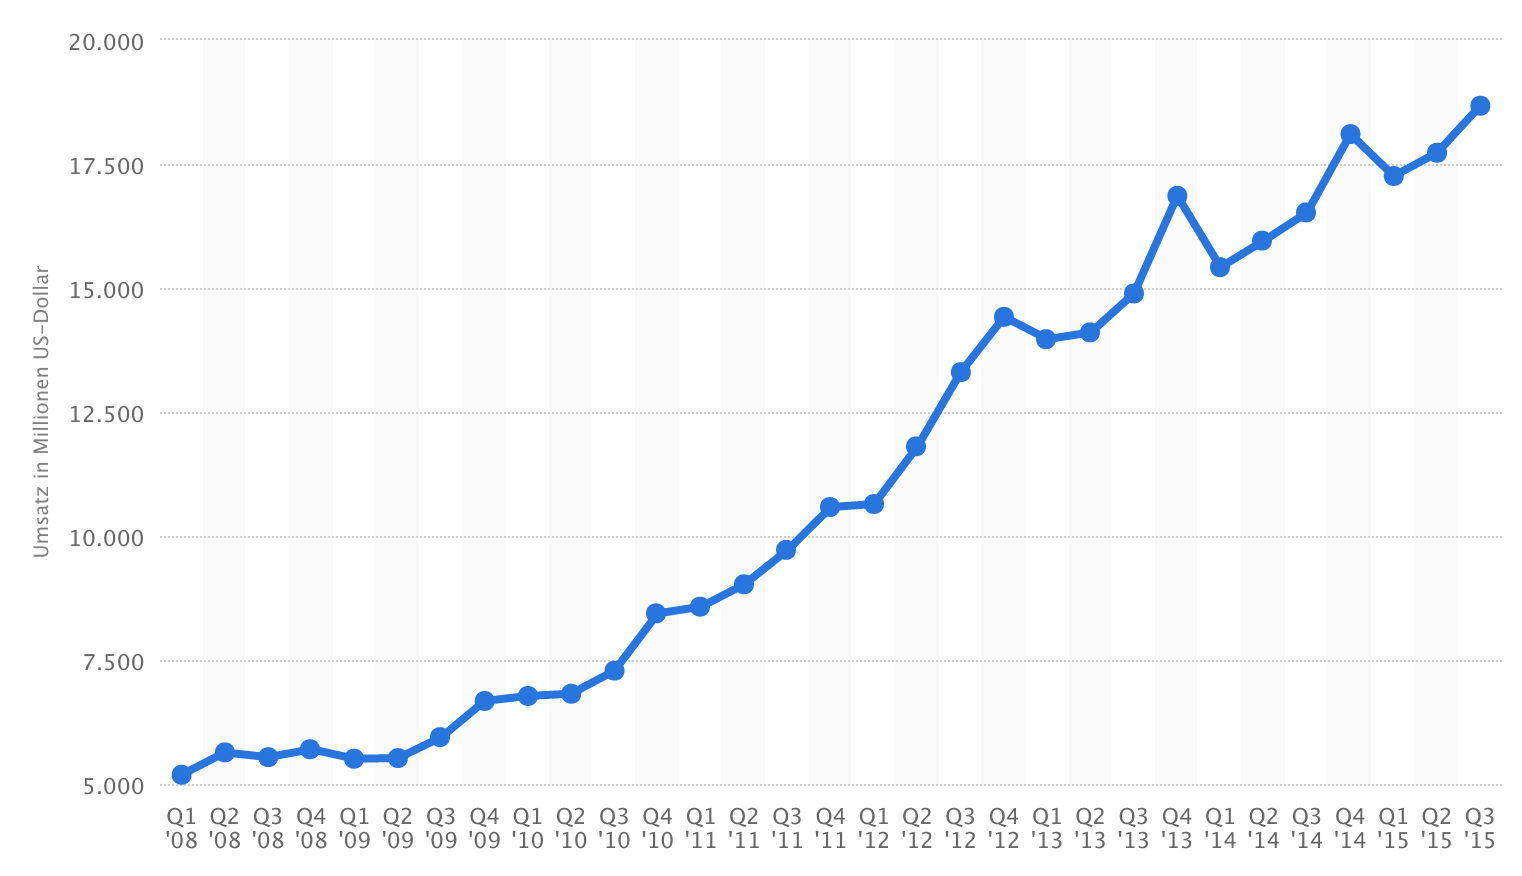
\includegraphics[width=0.9\textwidth]{../graphics/images/google_revenue.png}
	\caption{Revenue of Google in Mio. USD, © 2016 Statista, Source: \url{http://de.statista.com/statistik/daten/studie/154635/umfrage/umsatz-von-google-quartalszahlen/}
}
\end{figure}

\subsection{Open Source and Software as a Service (SaS)}
\label{sec:sas}

Many companies are implementing OSS as a part of their software service nowadays. This means, software services are usually offered through a platform (which is the internet by default). The terms \textit{Software as Service (SaS)}, \textit{Cloud Services} and \textit{Cloud Computing} imply that the service is only available via remote rather than installed as local software. Thus, SaS is rather rented than licensed (\cite{buxmann2008software}) and, compared with traditional locally installed software, profit is generated by leasing the software and service to the user.

The range of open and closed source code behind software services differs widely. Server side components and frontend modules often rely on OSS technologies \footnote{for example: many services using OS databases like MariaDB or PostgreSQL for data storage}. Because most SaS-APIs only allow receiving and returning (processed) users' data, those closed server-side processes make studying executed code hard or even impossible. Thus, the user is neither able to determine what the software really does nor able to change (and redistribute) it (\cite{WhatDoesThatServerReallyServe:online}). Therefore, this approach is widely against the initial thoughts of free software.

Moreover, cloud computing aims to force people to buy lock-in systems that will increase costs over time (\cite{CloudComputingIsATrapWarnsGnuFound:online}). To fill the gap of lacking copyleft on SaS, the free software foundation published the GNU Affero GPL in 2007 (\cite{GNUAfferoGeneralPublicLicense:online}) which demands a download link to the source code on hosted services running the affected software.

Beyond closed-source SaS-providers other companies like \textit{GitLab} (\cite{gitlabraises1.5million:online}) or \textit{ownCloud} (\cite{diycorporatecloudwithowncloud:online}) publish their entire server- and client-side software as OS. Profit is generated by providing enterprise editions (\cite{gitlabraises1.5million:online}; \cite{ownCloudServerOrEnterpriseEdition:online}; \cite[p.148]{van2014gitlab}) \footnote{the enterprise edition does not necessarily differ in features rather than then in support features for the service itself} for instance. Other companies publish and maintain specific libraries or components as OS \footnote{for example: facebook initiated React (\cite{reactnativeannouncement:online}) and uses React Native (\cite{reactnative:online}) in multiple production apps (\cite{reactnativegithubreadme:online})}. The latter is common practice for (larger) technology companies like Google, Microsoft, facebook or Amazon.


\subsection{Open Source and Open Innovation}
\label{sec:open_source_and_open_innovation}

OSS can be regarded as process innovation (\cite{bonaccorsi2003open}) with a connection to open innovation. Information to solve a problem can be sticky and opening innovation can help to solve the problem of sticky information (\cite{von1994sticky}). Open Innovation implies that valuable ideas may come from the inside or outside of a company \cite[p.43f]{chesbrough2006open} and let to the assumption that exploration and exploitation of internal and external ideas lead to better innovation. Using the term "openness" according to \cite{chesbrough2003logic}, "open innovation is a paradigm that assumes that firms can and should use external ideas as well as internal ideas, and internal and external paths to market, as firms look to advance their technology". Thus, companies can turn (technology regarded) ideas from inside and outside the company to profit (\cite{dahlander2010open}).

For the need of companies to connect "Open Innovation" with "Open Source",  \cite{dahlander2010open} give the following reasons:

\begin{itemize}
  \item Social and economic changes in working patterns:
	\begin{itemize}
		\item today employees are seeking more often portfolio careers than a single employer for lifetime
		\item OS commitment builds a better portfolio
	\end{itemize}
  \item Globalization:
	\begin{itemize}
		\item allows increasing division of labor
		\item enables working on distributed channels on source code
	\end{itemize}
  \item Intellectual property rights (IPR), venture capital (VC) and technology standards allow for organization to trade ideas
  \item Software and technology:
	\begin{itemize}
		\item changes the minimum efficient scale of production
		\item allows new ways to collaborate
		\item coordinates across geographical distances
	\end{itemize}
\end{itemize}

As follows, \textit{Open Source} and \textit{Open Innovation} are related terms since programming is a kind of innovation by creating new products (software) to solve (technical) problems.

\subsection{Open Source Collaboration of Firms with external Developers}

As stated in chapter \ref{sec:open_source_and_open_innovation}, OS developers are innovating users (\cite{von2005democratizing}): they evaluate, change and improve source code for their own purpose and solve problems by creating software for specific use cases. Usually they publish their innovations without claiming intellectual property rights and are driven by extrinsic and intrinsic motivation (\cite{hertel2003motivation}; \cite{hars2001working}; \cite{lakhani2002boston}).

Firms' investment in OS software and communities differs from the interest of (external) OS developers since firms expect a return of investment. Their intention of investment is mainly driven by economic, technical and strategic reasons (\cite{wichmann2002free}; \cite{henkel2006selective}). If firms acting in OS sections, conflicts with OS community members may occur due to different interests of contribution (see \cite{IveJustLiberatedMyModules:online} as example), license permissions (\cite{hars2001working}) and commercial intention. Forms of commitment by firms can be participating in software development, communication channels or in general by creating network effects through an "architecture of participation" \cite[p.22]{o2007web}.

But why do firms initiate OS projects and do maintain them even if they do not belong to their core business?

West and Gallagher identified the following benefits when organizations do sponsor OS projects \cite[p.13]{west2006challenges}:

\begin{itemize}
	\item helping to establish their technology as de facto standards (reduces the likelihood of having to re-implement other products to conform to competing standards)
	\item attracting improvements and complements that make the technology more attractive
	\item together, the innovation and complements enable the sale of related products
	\item generating mindshare and goodwill with the same audience that includes the potential
customers for these related products
\end{itemize}

As \cite{tsay2014influence} found out, contributions on GitHub by submitters with high status in the community and a stronger social connection to the project have a higher chance to get accepted. Besides, discussions of contributions have a social and technological factor. Contributions on established projects are harder to be accepted (\cite{tsay2014influence}) which may occur trough higher communication costs. In addition, employed developers who work for longer periods on firms' initiated OS projects have a higher reputation in the community, more power of control on contributions and larger influence of project's (technical) design and advancement.

Consequently, firms may receive indirect (nonmonetary) return of investments if they initiate and maintain projects that are not primary relevant for (monetary) revenue. Better reputation and establishment of software technology with more success are such returns as well as coming across new potential employees \footnote{external developers are potential employees since they have project related knowledge and matching skills}.

\subsection{GitHub as Host for observed Projects}

GitHub is the largest social coding repository and hosts over 35 Mio. repositories by 14 Mio. people (\cite{AboutGitHubPress:online}; \cite{HowGitHubConqueredGoogleMicrosoftAndEveryoneElse:online}). It was successfully used as data source in several other studies before (\cite{vasilescu2013stackoverflow}; \cite{tarrell2016GenderBiasInOpenSource}; \cite{dabbish2012social}; \cite{thung2013network}) and allows to query project related metadata. Moreover, all popular firms do publish their OS projects mainly on GitHub because it offers extended enterprise support (\cite{IntroducingGitHubEnterprise:online}) \footnote{against payment of a fee, \url{https://enterprise.github.com/features}} beside it's popularity for free and public accessible projects.

\subsection{Increasing commitment of Companies to Open Source}

\subsubsection{As an example of developing a common approach: Microsoft and Open Source}

Between the late 90s and the beginning of the century Microsoft was widely known for it's rigorous distaste towards OS licenses, OSS and especially the \textit{GNU/Linux} system. At this time Microsoft's core product and cash cow was Microsoft's operating system Windows (\textit{MS Windows} for clients \& \textit{MS Windows Server}) and \textit{Microsoft Office} \cite[p.2]{reifman2007microsoft}. In other words, Microsoft got threatened by OSS. This was regarding particular Linux as client and server operating system and \textit{OpenOffice} (nowadays widely known as fork \textit{LibreOffice}). This may be one of the reasons why former Microsoft CEO \textit{Steve Ballmer} regards \textit{Linux} (and it's GPL license) in 2001 as cancer that attaches itself in an intellectual property sense to everything it touches (\cite{ballmerlinuxcancer:online}).

Since user interaction with the operating system shifted from local machines (i.e. locally installed software on stationary computers) to the internet (using software services in the web browser and on mobile devices, as described in chapter \ref{sec:sas}), Microsoft couldn't defend its dominant position and lost market shares in the last decade (\cite{MicrosoftWindowsOEMandOfficeRevenueIsDownAsCloudGrows:online}).

By failing to defend the dominant position of their proprietary software, \textit{Microsoft} started to change their strategy over the last decade and increased their commitment in OSS. As \textit{Sam Ramji} already stated in 2008 (\cite{microsoftosstrategy2008:online}), \textit{Microsoft} has realized to include \textit{Linux} (i.e. other OSS and OS based services) as a vertical product integration in a heterogeneous environment on top of \textit{Windows}. This strategy of mixing OSS with proprietary software (\cite{mixingosandproprietarysoftware:online}) is common practice in technology companies nowadays.

In 2014 \textit{Microsoft} announced to publish their programming language and enterprise framework \textit{.NET} as open source (\cite{msnet2015os:online}). This step was just one of their latest upcoming OS commitments and facing towards the OS community (see \cite{microsoftchakracoreonline:online} as one of the latest examples).

Finally, \textit{Microsoft} moved in 2015 most of its OS projects from codeplex (their own OS hosting service) to \textit{GitHub} (\cite{msmovingtogithub2015:online}). With this step \textit{Microsoft} tries to reach the vibrant OS community (of \textit{GitHub}) and indicates that they want to be an active part of it. Currently, Microsoft's GitHub account contains more than 370 projects with 1,138 organizational developer profiles (external developers are excluded) \footnote{Retrieved \nth{9} January 2016}.

\subsubsection{GitHub's Atom Editor and Microsoft's Visual Studio Code as example for technology exchange between firms and collaboration with the OS community}

In 2011 \textit{GitHub Inc.} \footnote{to "distinguish" between the company and the community, we will use \textit{GitHub Inc.} for the company; but the transition is seamless sometimes} employee \textit{Corey Johnson} and \textit{GitHub} founder \textit{Chris Wanstrath} started building the \textit{Atom editor} (hereafter referred to as \textit{Atom}) as closed source project inside the \textit{GitHub} company (\cite{AtomV1:online}). \textit{GitHub} conceived the \textit{Atom} in February 2014 to the public (\cite{IntroducingAtom:online}). In May 2015 they published its source code (\cite{AtomIsNowOpenSource:online}) under the \textit{MIT License}. The idea of the \textit{Atom} is to be a "zero-compromise combination of hackability and usability" and therefore a rival software product to other closed source / commercial editors like \textit{Sublime}, \textit{Apple's XCode} and \textit{Microsoft's Visual Studio}. The feedback of the OS community was widely positive and \textit{Atom} gained quickly considerable attention  (\cite{AtomIsJustGettingStarted:online} and \cite{AtomReachesOneMillionActiveUsers:online}).

One key feature of \textit{Atom} is its modularity, which allows customization through "packages" (i.e. "plugins"). Each plugin is customized for specific software development needs. The format of packages and themes was previously introduced by \textit{Sublime}, which holds a large repository of plugins. Thus, all \textit{Sublime} plugins can easily be converted to \textit{Atom}
\footnote{\url{https://discuss.atom.io/t/convert-sublime-grammar-to-atom-grammar/14843}}.
In addition, the introduction of \textit{apm} (\textit{Atom Package Manager} \footnote{\url{https://github.com/atom/apm}} as central software provider for those plugins enabled a new software ecosystem for the editor and accelerated the acceptance of converting, building and deploying new plugins for \textit{Atom} by the community.

\begin{table}[!h]
\centering
\begin{tabular}{rlllll}
  \hline
 & Themes & Packages & Users & Authors & Downloads \\
  \hline
Atom & 1,008 & 3,496 & - & - & 32,79M \\
  Sublime & 295 & 3,426 & 4,6M & 2,477 & - \\
   \hline
\end{tabular}
\caption[Available Plugins for Atom Editor and Sublime Editor]{Available Plugins for \textit{Atom Editor} and \textit{Sublime Editor}; Retrieved on: \nth{21} January 2016 \protect\footnotemark}
\label{tbl:atomsublimeplugins}
\end{table}

\footnotetext{\ \ Source: \url{https://atom.io/packages}, \url{https://packagecontrol.io/stats}, \url{http://colorsublime.com}}

A year after the initial release of \textit{Atom}, \textit{Microsoft} announced its free and open source editor \textit{Visual Studio Code} (\textit{VSC}) (\cite{MicrosoftLaunchesVisualStudioCode:online}). \textit{VSC} is a code editor with similar look-and-feel, features and ideas of \textit{Atom}, but initiated by \textit{Microsoft}. Moreover, \textit{VSC} is based on \textit{Electron} (\cite{electroncrossplatformapps:online}) and \textit{React} - both are OS technologies by \textit{GitHub Inc.} and \textit{facebook} respectively and core technologies of  \textit{Atom} as well.

This makes \textit{VSC} to a rival product with the potential to substitute \textit{Atom}. Using \textit{Electron} and some other core libraries as foundation, \textit{VSC} guarantees interoperability of \textit{Atom's} plugins on its editor. In November 2015 \textit{Microsoft} finally published \textit{VSC} as open source likewise  (\cite{VSCodeIsOpenSource:online}).

\textit{GitHub Inc.} and \textit{Microsoft} are aware that the editor gets only established with a variety of plugins (see table \ref{tbl:dataofvscodeandatom}) and with an active community. The reason is that establishing software standards is to some degree a Winner-Take-All market. Once a standard is established in the community (here an editor with a specific API and package format) the development of "plugins" will be successful, too.

This example demonstrates how two firms published initially closed source developed software as open source: \textit{Atom} (\textit{GitHub Inc.}) and \textit{VSCode} (\textit{Microsoft}). Both editors are heavily using OS libraries as technical foundation.

Altogether, Microsoft's editor is a good example of

\begin{itemize}
	\item using OS technology of competitors (\textit{GitHub Inc.}, \textit{facebook} and \textit{Instagram})
	\item as foundation to build OSS for the community
	\item with plugins and code contribution by the community and developers by competitors
\end{itemize}

\textbf{Interpretation:} The reason why both firms decided to publish their projects as open source may be that the OS developers are their target customers (\cite{IntroducingAtom:online}), community members and potential employees. By providing technologies for the community, both firms will improve their reputation in the developer community. Furthermore, upcoming projects will be easier accepted by external developers, more likely successful and establishing software technology in future might be more feasible in a smaller amount of time.

\textit{A further analysis of "Atom" and "VSC" ("Microsoft" and "GitHub Inc." respectively) can be found in chapter \ref{sec:atom_vs_vsc} on page \pageref{sec:atom_vs_vsc}}

\clearpage
\subsection{Forms of Participation on GitHub Projects}
\label{sec:forms_of_participation_on_github}

\begin{figure}[!h]
	\centering
	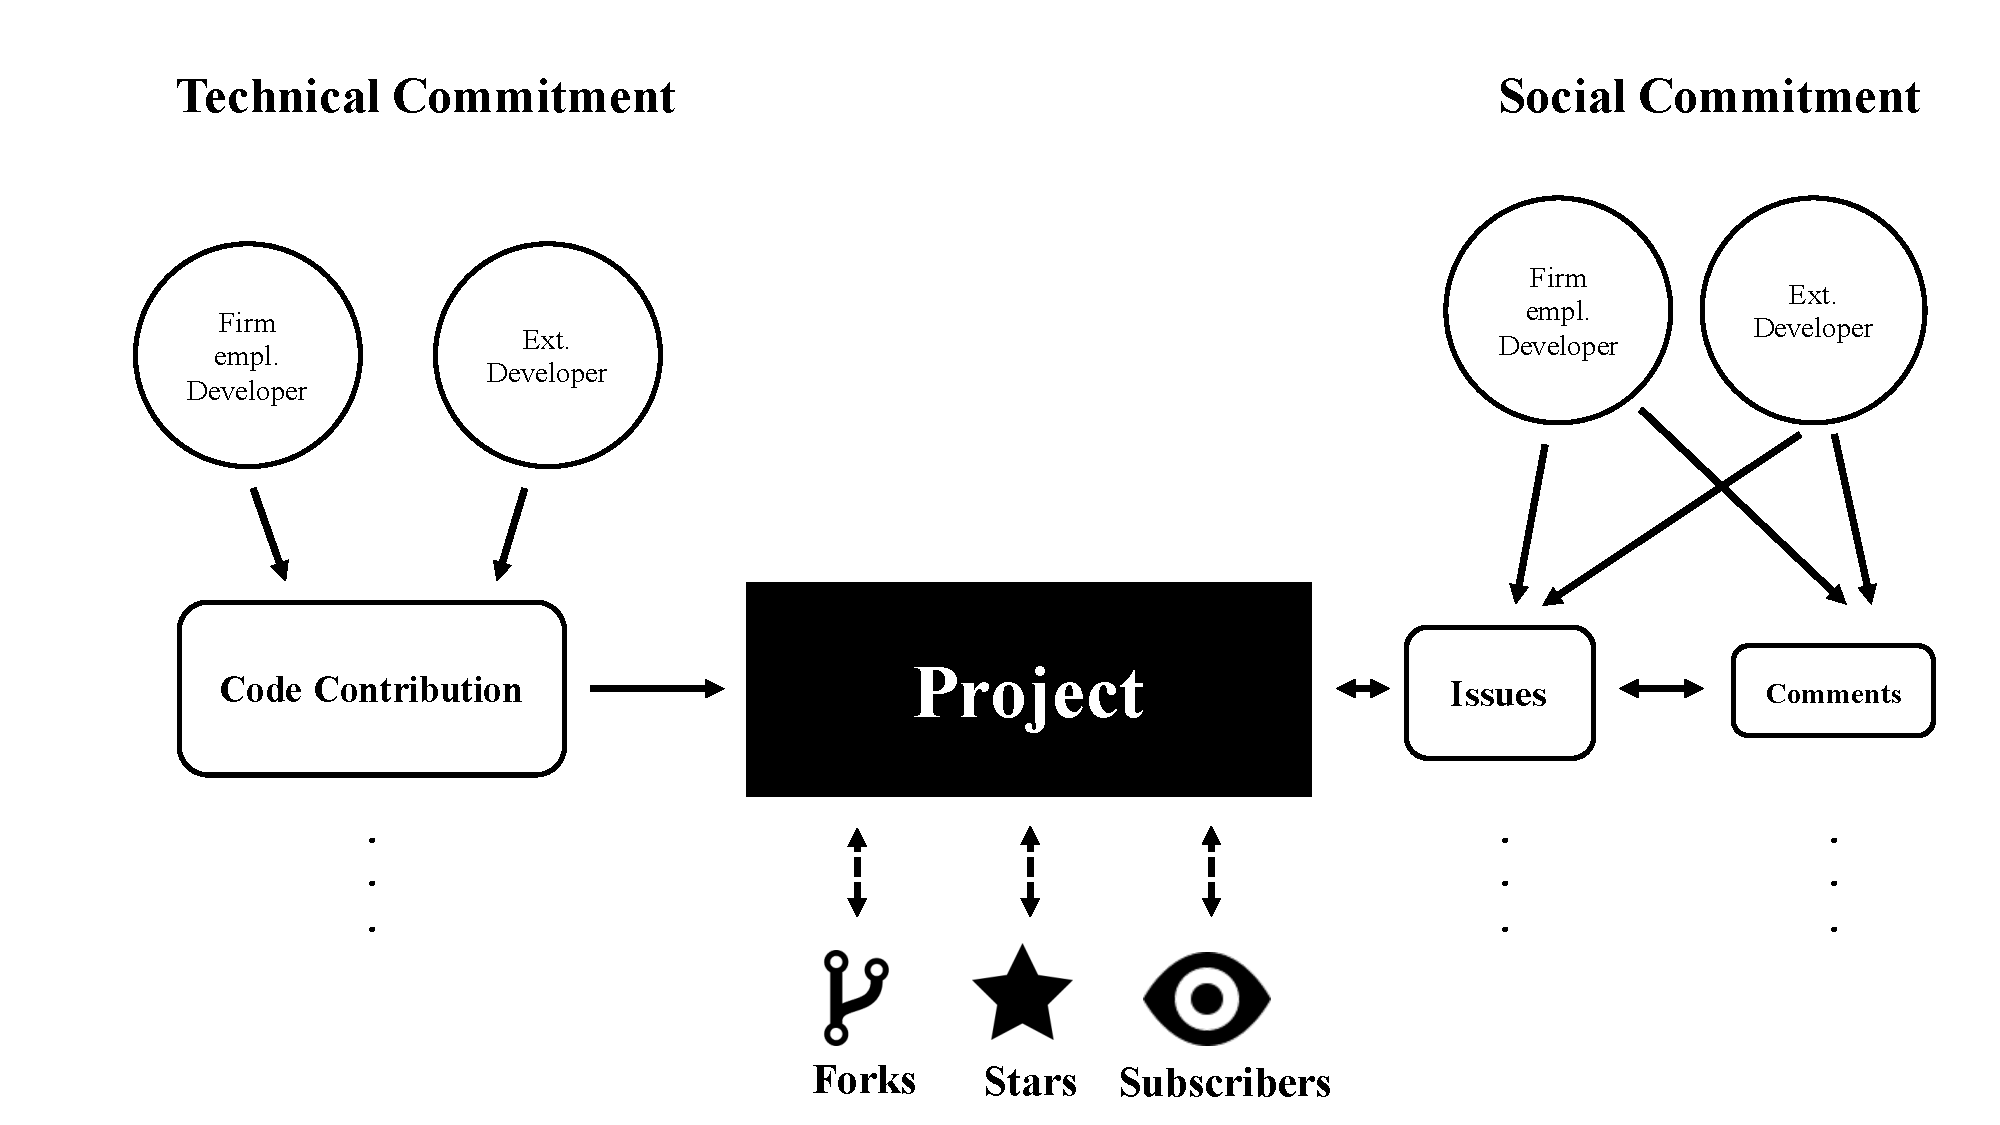
\includegraphics[page=1,scale=0.45]{../graphics/figure_contribution.pdf}
	\caption{Technical and social Commitment in GitHub Projects}
	\label{fig:forms_of_commitment}
\end{figure}

GitHub allows direct and indirect participation. This implies that every user can participate with minimum action (indirect) and active contribution (direct).

The following technical and social participations are possible:

\begin{itemize}
	\item Code Contribution (direct)
	\item Creating Issues (direct)
	\item Participation by commenting on Issues (direct)
	\item \textit{Fork}, \textit{Subscribe} and \textit{Star} project (indirect)
\end{itemize}

Use and interpretation of these attributes will be explained in chapter \ref{sec:social-success-metrics} on page \pageref{sec:social-success-metrics}.

\clearpage
\subsection{Linear and Logistic Regression Models}

The empirical analysis uses \textit{Linear \& Logistic Regression Models}. According to Seber and Lee we can describe the linear models of the study as follows \cite[p.35]{seber2012linear}:

\begin{align}
	 \text{lm}_{j} &: y_{\text{j}_{i}} &= \beta_{j_{0}} + \beta_{j_{i}} x_{j_{i}} + \dots + \varepsilon_{j_{i}} \\
	 & & x : \textit{explanatory variable} \nonumber \\
	 & & \varepsilon : \textit{fluctuation} \text{ or } \textit{error} \nonumber \\
	 & & \beta : \textit{unknown parameter} \nonumber \\
	 & & \text{lm} : \textit{linear model} \nonumber \\
	 & & \forall i \in \textit{observations} \nonumber \\
	 & & \forall j \in \textit{linear regression models} \nonumber
\end{align}

The independent and dependent variables will be different regarding to model assumptions. In particular \textit{Ratio} (share of contribution by internal developers) and \textit{Age} will be set as independent variable, \textit{share of contribution by external developers} and \textit{Top Project} set as dependent variable. \textit{Firms} and \textit{Programming Languages} will be used as dummy variables in some models.

Because \textit{Top Project} is $\in \{0, 1\}$, the \textit{logit model} is used in this case \cite[p.23]{hilbe2009logistic}:

\begin{align}
	 \mu_{j_{i}} = \frac{ 1 }{ 1 + e^{-x_{j_{i}} \beta_{j_i}} } \\
	 & & \mu : \textit{fitted value} \nonumber \\
	 & & \forall i \in \textit{observations} \nonumber \\
	 & & \forall j \in \textit{logistic regression models} \nonumber
\end{align}

\subsection{Fitting Linear Mixed-Effects Models}

To consider effects within \textit{Firms} and effects within \textit{Programming Languages} some analyses will be handled additionally by \textit{Fitting Linear Mixed-Effects Models} \cite[p.13]{R_lme4}: \footnote{as mentioned in \cite[p.1]{R_lme4}, "mixed effects" denotes a model that incorporates both fixed- and random-effects terms}

\begin{align}
	\eta_{j} = X\beta_{j} + Z\gamma_{j} + \varepsilon_{j} \\
	& & \eta : \textit{known vector} \nonumber \\
	& & \gamma : \textit{unknown vector of random effects} \nonumber \\
	& & \beta : \textit{unknown vector of fixed effects} \nonumber \\
	& & \varepsilon : \textit{unknown vector of random errors} \nonumber \\
	& & \forall j \in \textit{linear mixed-effects models} \nonumber
\end{align}

\clearpage
\subsection{Hypotheses}
\label{sec:hypotheses}

Derived from motivation, theory and previous studies \footnote{\cite{hill2009idea}; \cite{dahlander2014open}; \cite{piezunka2013study}; \cite{dahlander2005relationships}; \cite{alexy2012managing}; \cite{tsay2014influence}; \cite{west2006challenges}; \cite{krishnamurthy2016peripheral}} we formulate the following hypotheses:

\begin{itemize}
    \item [\textbf{H 1}] Firm employees' participation affects the participation of external developers
		\begin{itemize}
			\item [\textbf{H 1.1}] If firm employees contribute source code more often, external developers do as well
			\item [\textbf{H 1.2}] If firm employees participate more often on issue threads, external developers do as well
		\end{itemize}
    \item [\textbf{H 2}] Firm employees' participation (in the beginning) affects the (later) success of firm-initiated open source projects
		\begin{itemize}
			\item [\textbf{H 2.1}] If firm employees contribute source code more often in the beginning, the project gets more successful
		\end{itemize}
		\item [\textbf{H 3}] If firm employees' contribution share is higher overall the more likely the project is popular
\end{itemize}


The analysis will contain code contribution (technical commitment) and participation on issues and comments on issues (social commitment) \footnote{whereby issue participation can also be technical in some cases}. Contribution will be measured with a "standardized contribution share" in respect of (social) success metrics and relations between firm employed developers and external developers. All hypotheses will be verified with firms' publicly available OS projects on GitHub.

\newpage
%%\input{methods}
%%\newpage
%%\%input{data}
%%\newpage
%%
\section{Results and Conclusion}
\label{sec:results}

All hypotheses are mainly confirmed by the empirical findings:

\begin{itemize}
  \item Through their code contribution firm employed developers have a strong positive impact on the code contribution of external developers
  \item Firm employed developers have a strong positive impact by participating on issues and comments in issues by causing more participation of external users
  \item The first year seems to be the most important time period for firm employed developers' participation: High contribution ratio in the beginning benefits popularity and success of the OS project in the long run
  \item The higher the overall share of contribution from firm employed developers, the more likely the project is successful and accepted by the OS community
\end{itemize}

Nevertheless, influence of higher participation of firm employed developers could not be verified ultimately on some continuous social metrics \footnote{\textit{Forks} and \textit{Number of Issues} on some models} which might be caused by broad difference of popularity and level of awareness between firms and software segments.

Beside the regression results we also receive interesting fringe insights: According to the frequency of commits with respect to daytime we can assume, that most firms and OS developers do work in USA, Canada and Europe. Also do external developers seem to be employed as well. Most developers commit source code at the usual working time period (9 a.m. - 5 p.m.) and "external developers" do not differ significantly from as "firm employed" classified developers. This would imply, that there is a stronger collaboration between firms than between firms and "libertine" developers.

\subsection{Implications and Managerial Advice}

Firms should initiate and invest \footnote{with funds and man-power} in their OS projects. The share of code contribution by firm employees should be very high - especially in the beginning - to achieve a broad acceptance by the OS community and developers on (rival) firms \footnote{contribution in the beginning can be interpreted as groundwork that needs to be done by firm employed developers to build a solid software foundation}. The return of investment will be a multiplier effect on commitment \footnote{via source code contribution and participation in communication channels} by external developers and a gain on level of awareness. Beside that, firms' OS commitment might lead to more cross-firm collaboration, improve employment of external developers and bring forward establishing new technologies in smaller amounts of time. If the share of firm employed developers is higher than usual, projects seem more likely to reach a certain degree of quality, maturity and attention. As result the community is willing to contribute their professional expertise for free to the project.

% As the selection of firms (by their number of popular projects) reveals, almost all well-known and favored software technology firms are represented.

\subsection{Further Research}
\label{sec:further_research}

The empirical data implies further research with respect to broader observations of firms and projects. By analyzing more firms and projects the hypotheses could eventually be applied more generally to software technology driven firms. Consideration of financial data of firms could reveal the impact of OS commitment on firms' revenue. And more sophisticated employees firm rating would help to investigate the coherence of OS commitment and quality of work environment. Furthermore, observations of network relations between firms, developers and users would improve the understanding of the importance of collaboration and exchange of knowledge.
%
% \begin{itemize}
%   \item observe all firms
%   \item firm financial data
%   \item firm / work place ratings by employees (developers)
%   \item collaboration between firm developers
%   \item measure firm reputation in open source communities (improves more OS commitment firm's reputation in the community / for potential employees)
% \end{itemize}

% \subsection{Outlook and Discussion}
%
% \begin{itemize}
%   \item further research (network effects, cross firm collaboration)
% \end{itemize}

% TODO: Results, Conclusion, Discussion


% Help tp Lontables
% Source: http://tex.stackexchange.com/questions/11380/how-to-repeat-top-rows-column-headings-on-every-page
% \documentclass{article}
% \usepackage{longtable}
% \begin{document}
% \begin{longtable}{ccc}
% \hline
% Column 1 & Column 2 & Column 3\\
% \hline
% \endhead % all the lines above this will be repeated on every page
% A & B & C\\
% A & B & C\\
% ... many lines of table ...
% \end{longtable}
% \end{document}
% --> \endhead
,
%%\input{conc}

\clearpage
\newpage
%\addcontentsline{toc}{section}{Data}
\section{Data}
\label{sec:data}

In the following chapter, the collection, processing and validation of the relevant data will be explained. The empirical data is collected from public projects on GitHub until February 2016 \footnote{collected during the period from December 2015 to February 2016}. Repositories' related activity data is analyzed from 2011 to 2015.

Beside the selection of languages (see chapter \ref{sec:selection_of_programming_languages}) and firms (see chapter \ref{sec:firms_are_relevant_commercial_organizations}) all analyzed observations are unfiltered \footnote{unless stated otherwise} and contain the full available range of public available firms' OS projects.

\textit{Git} is an OS distributed version control system. It is published and developed by the \textit{Linux} development community (including Linus Torvalds, the creator of \textit{Linux}) since 2005 \cite[p.31]{chacon2014pro}.

\subsection{Data Sources and Open Data Approach}

All analyzed data is collected from the following public and free available data sources:

\begin{itemize}
	\item [\textbf{GitHub API:}] Project data, issues and issue comments
	\item [\textbf{Git repository:}] Code contribution
	\item [\textbf{Glassdoor API:}] \footnote{\url{https://www.glassdoor.com/developer/index.htm}} Firm and employee's ratings
	\item [\textbf{GitHub Archive:}] \footnote{\url{https://www.githubarchive.org/}} Time-referenced data for user events (time period 2011 - 2015)
	\item [\textbf{GHTorrent Project:}] \footnote{\url{http://ghtorrent.org/}} User data (email, location, company and full-name)
	\item [\textbf{LinkedIn Websearch:}] Manual classification for developer employments
\end{itemize}

External data is received as JSON files (\cite{bray2014javascript}) and converted to the CSV format (\cite{shafranovich2005common}) for better processing possibilities in \textit{R}. All data can be downloaded and observed through a git repository \footnote{\url{https://git.zeitpulse.com/philipp/masterthesis-data/tree/master}}.

\clearpage
\subsection{Selection of Programming Languages}
\label{sec:selection_of_programming_languages}

To specify a proper selection of relevant OS projects we need to define a list of popular programming languages.

The most used programming languages on \textit{GitHub} \footnote{\textit{Visited 12.01.2016:  \url{https://github.com/search?o=desc&q=stars:\%3C1}}} are listed in table \ref{tbl:github_language_distr_top_repos} (\cite{GitHubTrendingLanguages2015}). The figures reflect the overall ranking of programming languages in OS (\cite{GithubsTopCodingLanguagesShowOpenSourceHasWon:online}) and integrates close enough to the \textit{TIOBE index} (\cite{TIOBE2015}) and \textit{Programming languages used in most popular websites} on \cite{ProgrLangPopWeb2015}. Excluded languages are \textit{Shell} and \textit{CSS} since \textit{Shell} is a UNIX command line interpreter and neither used for building regular web services nor for building software in the proper sense \footnote{ \url{http://www.rpi.edu/dept/arc/training/shell/slides.pdf}} and \textit{CSS} is a markup language and not a programming language.

The replacement of \textit{Shell} and \textit{CSS} with the \textit{GO language} seems to be reasonable (see \cite{JavaReignsButGoLanguageSpikesInPopularity:online}, \cite{ThePopularityOfGo:online} and \cite{WhyGooglesProgrammingLanguageCanRivalJava:online} for possible reasons). The selection excludes the "rising stars" of OS programing languages \textit{Scala, Hack} and \textit{Swift} since the popularity, spreading and age of those languages is too little for the observation.

The following 10 languages (in alphabetically order, grouped by programming language family) are finally selected:

\begin{itemize}
	\item C, C\#, C++, Objective-C
	\item Go
	\item Java
	\item JavaScript
	\item PHP
	\item Python
	\item Ruby
\end{itemize}

The exact number of projects according to \textit{Stars} and \textit{Forks} can be looked up in table \ref{tbl:github_language_distr_top_repos} and figure \ref{fig:github_popular_programming_languages} respectively.

The usage of programming languages in projects differ between firms. Some firms promote their own programming languages (e.g. \textit{Google} uses \textit{Go} / \textit{Microsoft} uses \textit{C\#} more often than usual) or use specific languages according to their field of application (e.g. \textit{GitHub Inc.} uses \textit{Ruby}). Figure \ref{fig:programming_language_use_by_firms} and
\ref{fig:languages_used_in_projects} illustrate the usage of the 10 selected programming languages in "Top Projects" and "Residual Projects" \footnote{terms will explained on page \pageref{sec:top_and_residual_projects}} according to firms.

\begin{figure}[!h]
	\centering
	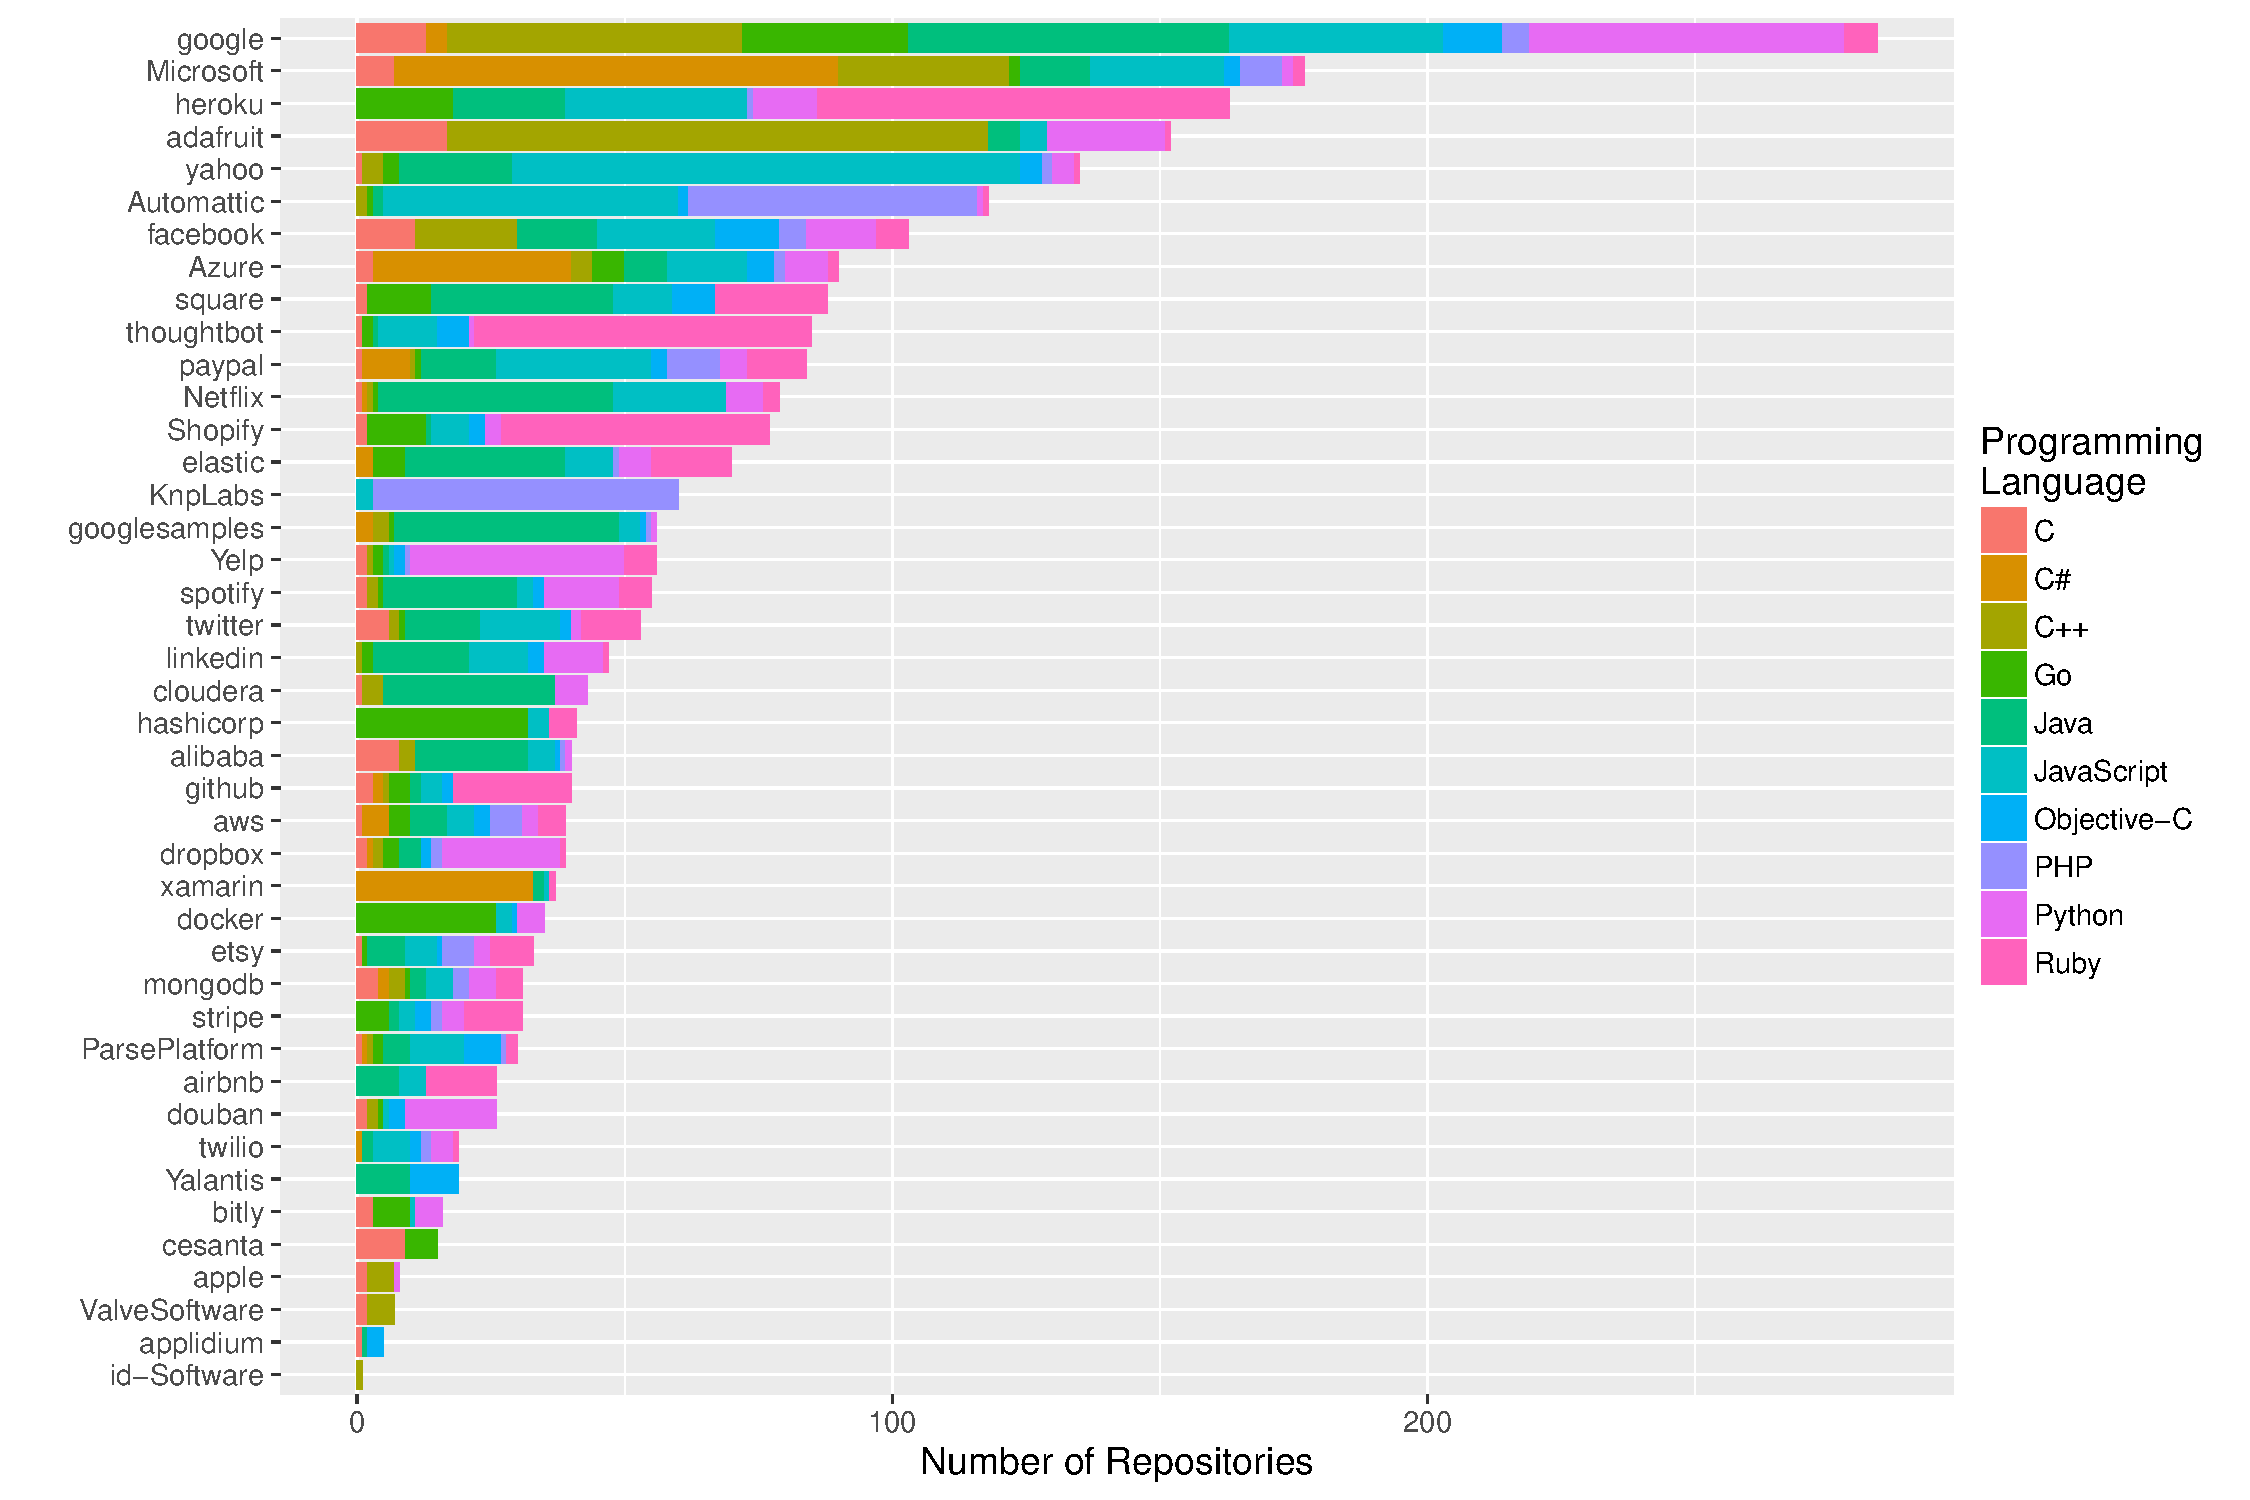
\includegraphics[page=1,scale=0.45]{../graphics/intro/programming_language_use_by_firms.pdf}
	\caption{OS Projects of Firms and the Programming Languages they are written in}
	\label{fig:programming_language_use_by_firms}
\end{figure}

\begin{figure}[!h]
	\centering
	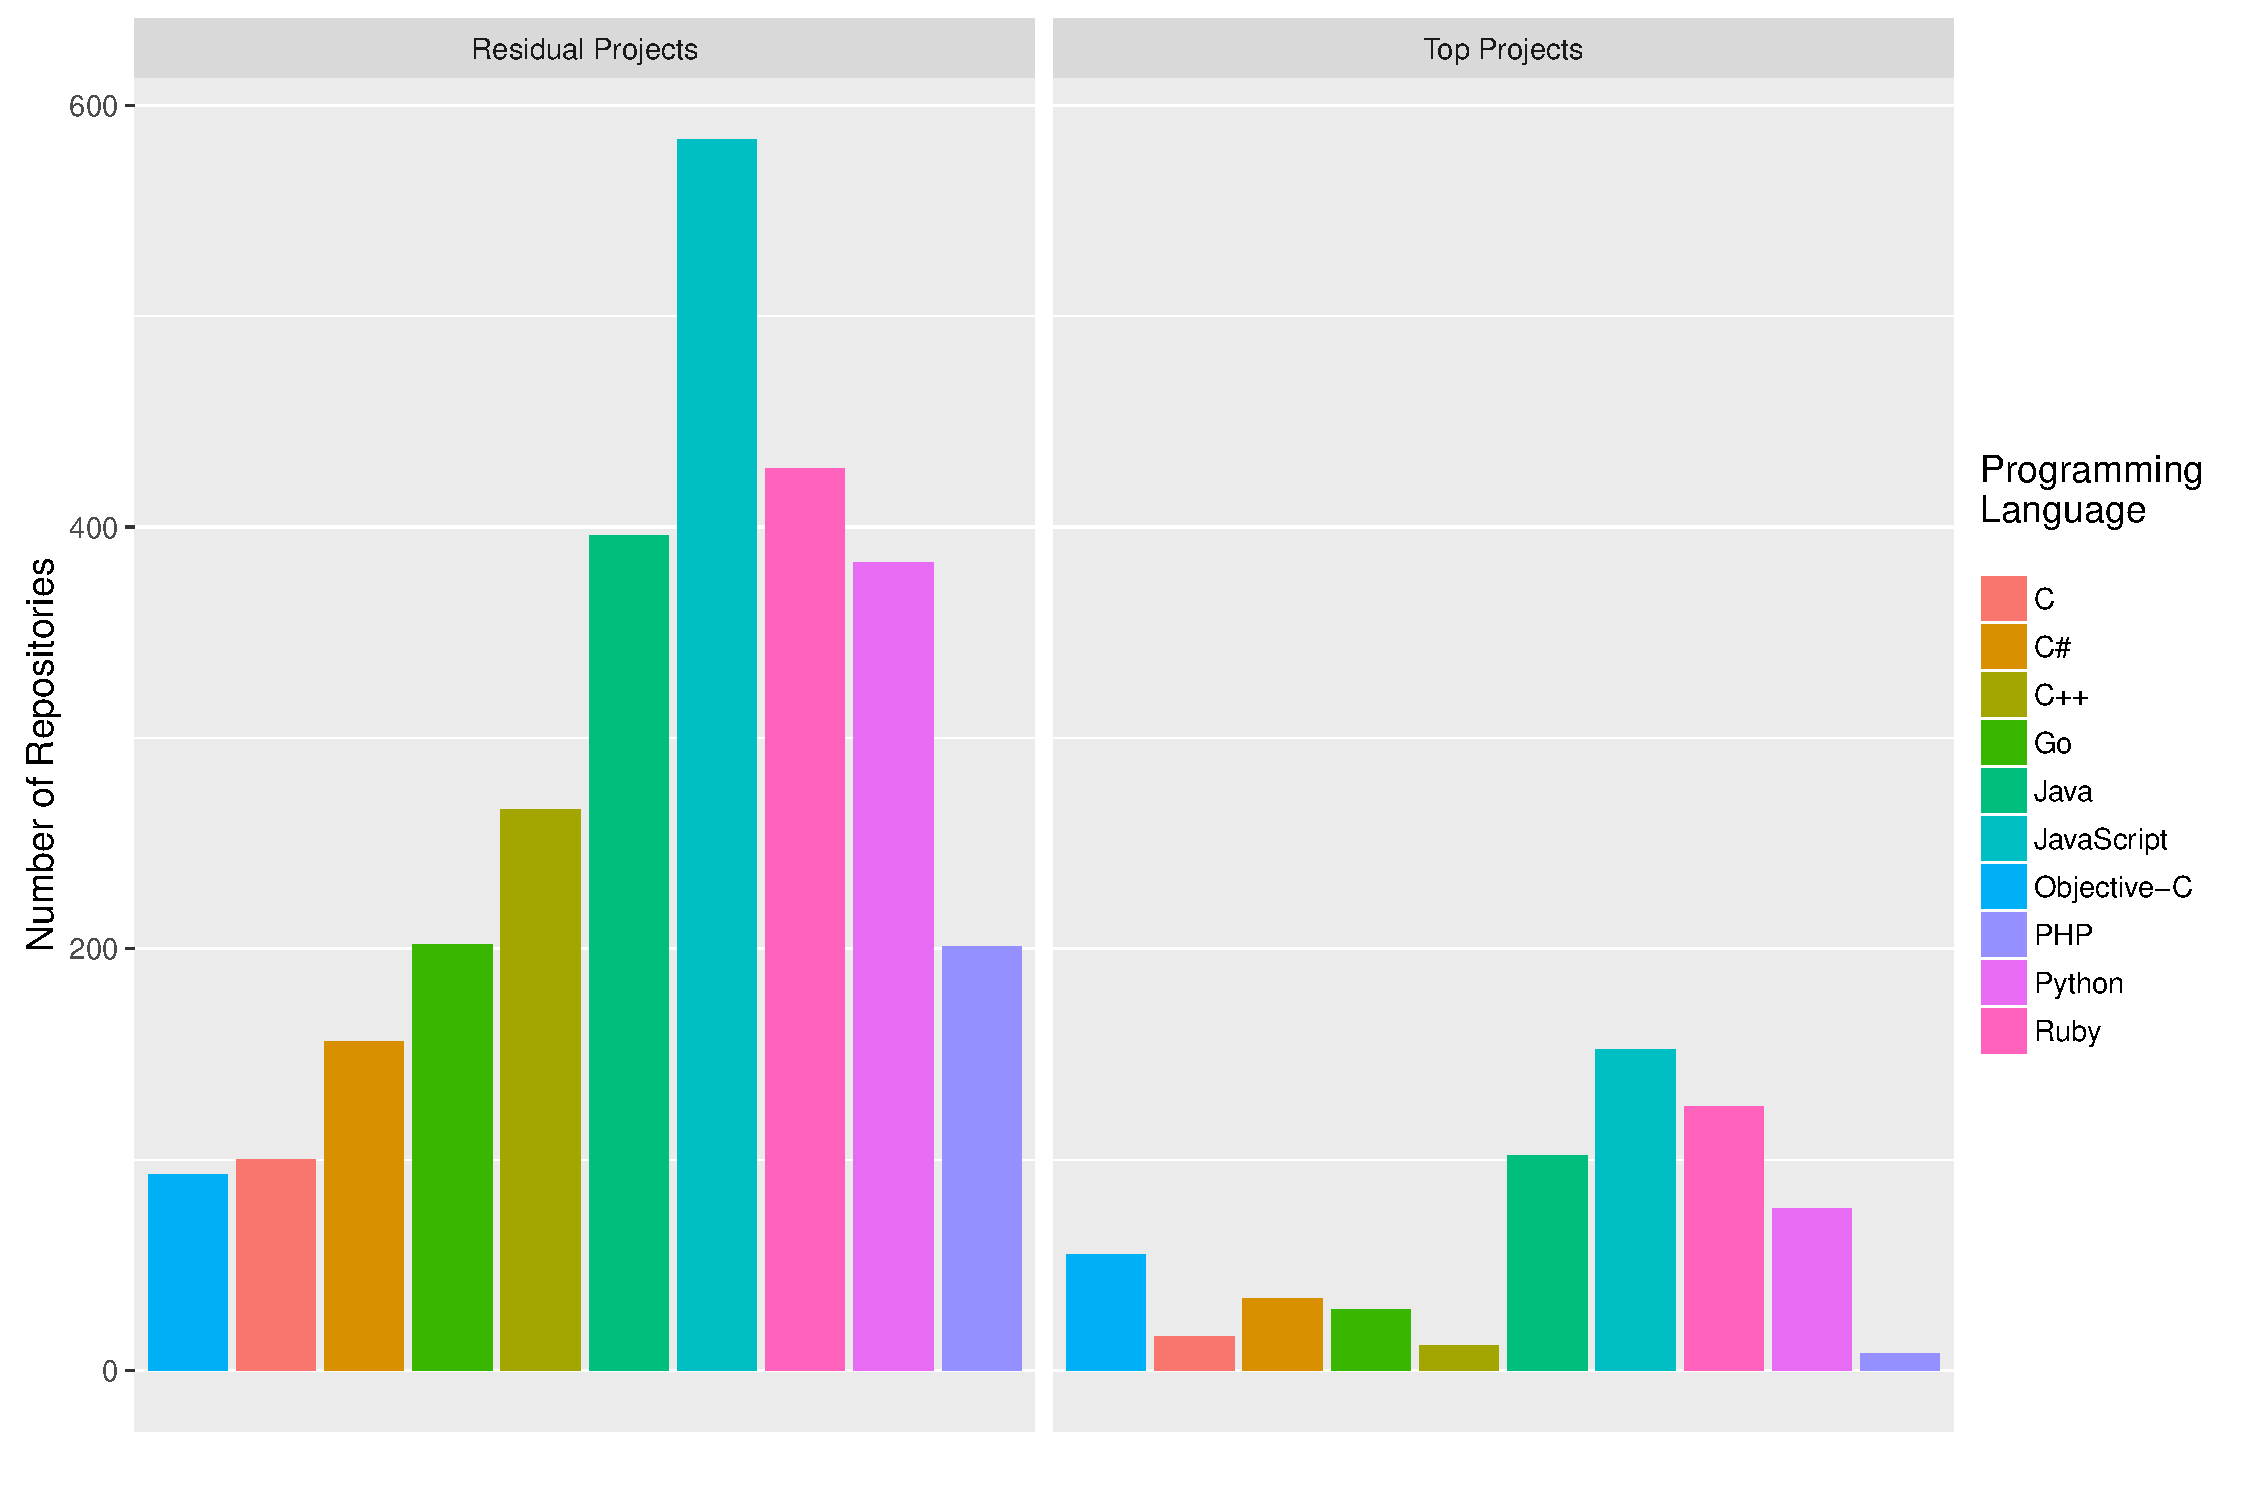
\includegraphics[page=1,scale=0.45]{../graphics/intro/languages_used_in_projects.pdf}
	\caption{Programming Languages which are used in \textit{Top Projects} and \textit{Residual Projects}.}
	\label{fig:languages_used_in_projects}
\end{figure}

\begin{table}[!h]
\centering
\begin{tabular}{lll}

\hline
\textbf{Programming language} & \textbf{Stars} & \textbf{Forks} \\ \hline
JavaScript        & 252891        & 134294         \\
Python            & 132995        & 74924          \\
Java              & 115249        & 83361          \\
Ruby              & 105547        & 55153          \\
PHP               & 97112         & 57332          \\
C                 & 59920         & 36506          \\
C++               & 53706         & 33105          \\
Objective-C       & 44734         & 24845          \\
C\#               & 35859         & 22157          \\
Shell             & 36874         & -              \\
CSS               & -             & 21637          \\ \hline
\textbf{Sum}      & \textbf{934887}     & \textbf{733789}         \\ \hline

\end{tabular}
\caption{Programming Languages with projects' \textit{Stars} and \textit{Forks} (\textit{Retrieved: 12.10.2016})}
\label{tbl:github_language_distr_top_repos}
\end{table}


\clearpage

\subsection{Restrictions of Data Collections}

All measurements and analyses are made under the following restriction: GitHub repositories' social data (\textit{stargazers}, \textit{forks}, \textit{contributors}, …) can only be measured with the actual values, i.e. cross-sectional data. For that reason, these attributes are query able through the GitHub API (\cite{GitHubApi}) with the possibility of sorting. However, querying and analyzing time series of GitHub event data is possible through the GitHubArchive (see \cite{grigorik2012github}; \cite{AnalyzingMillionsOfGitHubCommits:online}; listing \ref{lst:githubusersandprojectscount}) having events with the verbs \textit{watch} (mostly called \textit{subscribing}) and \textit{fork}. As mentioned in the beginning, the available time period of user activities is from 2011 to 2015 \footnote{GitHub itself exists since 2007 (\cite{GitHubCEOAndCo-FounderChrisWanstrathKeynoting:online})}.

\subsection{Social-Success-Metrics of git Repositories}
\label{sec:social-success-metrics}

A \textit{git repository} (sometimes also called \textit{git project} or \textit{git repo}, where \textit{git} is an optional term) provides the following statistics by default:

\begin{itemize}
	\item date and time of commits (commits are code contributions)
	\item name and email of the author (authors are developers)
	\item time zone location of the contributor (via the date-time property)
	\item code changes and action \footnote{an action may be a regular \textit{code commit}, \textit{code merge} or basic file operation (like rename, delete, copy or create file)}
\end{itemize}

A GitHub project has the following social metrics (terms will be described in the paragraph below):

\begin{itemize}
	\item Stars / Stargazers
	\item Subscribers (sometimes also called "Watchers")
	\item Forks
	\item Open and closed Issues
\end{itemize}

Finally, we get the following metrics of interest:

\begin{itemize}
	\item Number of Stargazers, Subscribers and Forks
	\item Number of Code Commits
	\item Number of Contributors
	\item Number of Issues and Comments on Issues
\end{itemize}

\textbf{Stargazers} \footnote{derived "action" is \textit{Star}} are GitHub users / developers who mark a project with a star (\cite{GitHubStargazers}), similar to the ordinary "like button" on \textit{facebook}. The reason may be to mark this as one of your favorite projects or to show the initiator your interest in the project or idea.

\textbf{Fork} is a copy / clone of a git project (\cite{GitHubForks}) containing all previous code contributions until the moment of the fork event. Projects are forked either to collaborate with the origin project or to be resumed as an independent project \footnote{\textit{LibreOffice} is a fork of \textit{OpenOffice} which is continuing as independent project for instance}. The number of forks doesn't explain necessarily the activity of contributors nor the popularity. If you participate on a GitHub project by committing code (called \textit{pull request} \footnote{\url{https://help.github.com/articles/using-pull-requests/}}) with your GitHub account, this project will be forked into your account by default. The \textit{clone} and \textit{fork} actions are fundamental ideas of the decentralized approach of git (\cite{loeliger2006collaborating}).

\textbf{Subscribers} are users who get notified on important project activities (\cite{GitHubWatchers}). The term is similar to \textit{subscribing} on \textit{facebook} or \textit{following} on \textit{twitter}. \textit{Subscribing} may be considered as the most important indicator of active interest in projects (beside code contribution and issue participation).

\textbf{Issues} are communication threads (\cite{GitHubIssues}). Every issue can be \textit{open} or \text{closed} and labeled as \textit{feature request}, \textit{bug report}, \textit{idea} or \textit{code proposal} for instance. Issue threads are an exclusive collaboration feature of GitHub \footnote{\url{https://guides.github.com/features/issues/}} and not implemented in git itself.

In terms of \textbf{"Forms of Participation"} (see chapter \ref{sec:forms_of_participation_on_github} and figure \ref{fig:forms_of_commitment} respectively) we can roughly classify this (direct and indirect) user actions from "lower participation / activity" to "higher participation / acitivity". \textit{Stars} and \textit{Forks} can be interpreted as the lowest participation level because they do not influence projects' progress directly (everyone can \textit{fork} and \textit{star} a project without any direct "consequences"). Whereas \textit{subscribing} is more active (but still indirect), because it provides constant updates of the current project activities to the subscribing user.

The impact of internal (and external) contribution on these levels of participation has to be considered specifically. In general, higher-active responses are more important than lower-passive responses.

\clearpage
\subsection{Projects' Data Enquiry}

Due to GitHub API limitations (\cite{GitHubApiLimit}) we are only able to query 1000 results for each language. As mentioned before, only firm's initiated projects for the 10 most famous programming languages are interesting for the observation.

By querying the most popular 1000 repositories for each of the programming languages \footnote{for each language:  \url{https://api.github.com/search/repositories?q=language:$ProgrammingLanguage$&sort=stars&order=desc&per_page=100&page=1...10}, queried on 19.1.2016} we finally receive 10,000 repositories \footnote{\url{https://git.zeitpulse.com/philipp/masterthesis-data/tree/master/apidata/top_repos_by_language}} from 2858 different organizations \footnote{\url{https://git.zeitpulse.com/philipp/masterthesis-data/raw/master/csv/organizations.csv}}, sorted descending by listed "Top Repositories" for each organization \footnote{in the following top repositories or top projects are all projects listed in the top 1,000 search matches} (see table \ref{tbl:organizations_with_top_repos} on page \pageref{tbl:organizations_with_top_repos}).

This results in 2,858 organizations having 78,055 public repositories (see table \ref{tbl:rep_numbers_organization} for details  \footnote{\url{https://git.zeitpulse.com/philipp/masterthesis-data/raw/master/apidata/organizations_top_repos_restructured.json}}). By selecting the most relevant organizations \footnote{i.e. having at least 4 different projects in the search results of most popular projects on all 10 programming languages} we get 113 (share of 3.95 \%) relevant organizations \footnote{data source: \url{https://git.zeitpulse.com/philipp/masterthesis-data/raw/master/csv/repositories_details.csv}}. We can classify finally 58 relevant commercial firms (see table \ref{tbl:selected_commercial_firms} and chapter \ref{sec:firms_are_relevant_commercial_organizations}).

Evidently, closer examination of the data shows that nearly every commercial successful firm in the technology area has a public GitHub profile (see table \ref{tbl:commercial_successfull_firms_on_github_with_languages} on page \pageref{tbl:commercial_successfull_firms_on_github_with_languages}).
%
% \subsubsection{Top and residual Repositories}

\label{sec:top_and_residual_projects}

We classify \textbf{Repositories} as:

\begin{itemize}
	\item[\textbf{Top Repositories}] (sometimes also called \textit{Top Projects}), which were found the first 1,000 rank search result
	\item[\textbf{Residual Repositories}] are the remaining amount of repositories by each firm
\end{itemize}

All firms' projects that are classified in one of the 10 chosen programming languages and are not tagged as "fork" are relevant \footnote{Remark: Unfortunately, not all projects can be classified absolutely as \textit{fork} and \textit{not fork} since not all projects are tagged as such on GitHub itself}.

\begin{table}[!h]
\centering
\begin{tabular}{ll}
Popular / Top Repositories:  						& 10,000         	\\
Repositories by Organizations:		& 78,055					\\
Organizations:  									& 2,858          \\
Organizations with relevant Number of Top Repositories:  					& 113          \\
Commercial Organizations:  					& 58          \\
Share of relevant Organizations:  & \textbf{3.954 \%}		\\
Share of observed Organizations:  & \textbf{2.03 \%} \/ \scriptsize{(51.33 \%)}
\end{tabular}
%\hspace{\textwidth}
\caption{Top Repositories for selected Programming Languages on \textit{GitHub}. "Share of observed Organizations" are finally classified commercial firms (selection criterions will be explained in chapter \ref{sec:firms_are_relevant_commercial_organizations})}
\label{tbl:rep_numbers_organization}
\end{table}

\clearpage
\subsection{Firms are relevant commercial Organizations}
\label{sec:firms_are_relevant_commercial_organizations}
A firm is relevant for the study, if

\begin{itemize}
	\item it is a commercial organization
	\item uses at least one of its projects actively in their business
	\item it contributes source code to their own projects and to other OS projects
	\item it holds and uses a global web domain \footnote{an actively used web domain is important to classify firm employed and external developers}
\end{itemize}

The selection was done manually by evaluating the form of company, activity with employed developers and firms' business activity. Since the classification of commercial activity is qualitative, it is also based on ratings by employees on Glassdoor \footnote{\url{https://www.glassdoor.com/}} \footnote{\url{https://git.zeitpulse.com/philipp/masterthesis-data/tree/master/apidata/glassdoor/employers}}, which will be introduced in chapter \ref{sec:glassdoor_ratings}.

We will evaluate the repositories of these firms \footnote{\url{https://git.zeitpulse.com/philipp/masterthesis-data/blob/master/csv/repositories.csv}} and compare participation of firm employed and external developers.

The assessment of which organization is commercial and builds a business on its OS projects follows the assumption that:

\begin{itemize}%[a)]
	\item most projects are used by the firm in commercial context (like \textit{docker, aws} ...)
	\item the firm offers paid services for some of its project (like \textit{chef, Microsoft, } ...)
	\item the firm acts commercial - even the OS projects and their service is available for zero costs (like \textit{GitHub, facebook} ...)
\end{itemize}

\subsection{Structure of a git Project}

A git repository can roughly be described with the following attributes \cite[p.~32]{loeliger2012version}:

\begin{itemize}
	\item commits, tags and merges
	\item branches
	\item trees \textit{(not relevant here)}
	\item files / blobs \textit{(not relevant here)}
\end{itemize}

A detailed explanation of those attributes is not necessary because only \textit{commits} and \textit{branches} are relevant for the study and will be explained in the following chapters.

\subsection{Branches of Interest}

Each git repository contains different branches. Every branch can be a different working subtree (i.e. source code environment) of a project. We will only inspect the default branch of each project which is in most cases the \textbf{master branch}. The master branch is by convention the official branch containing all finally submitted and accepted code of a project \cite[p.~89-90]{loeliger2012version}. Some projects have different default branches (\textit{production} branch for instance) and will be scope of the observation if it is tagged as such on GitHub.

% \subsection{Used Programming Languages by Firms}

\subsection{Firms' License Usage}
\label{sec:firms_and_licenses}

Which kind of licenses firms are using might reflect their strategic and projects' commercial long-term intention respectively.

With the following segmentation (based on \cite{bonaccorsi2003licensing}) for the most used licenses of the observed repositories / firms, we can describe a spectrum from restrictive to permissive licenses. As figure \ref{fig:licenses_used_by_firms} illustrates: most firms use (very) permissive licenses (from green-blue to magenta) instead of restrictive licenses (red to orange) \footnote{which is in line with \cite{bonaccorsi2003licensing} and \cite{top20oslicenses:online}}. The reason might be simple: Permissive license avoid problems of the copy-left idea and enables future commercial (closed source) development.

\begin{figure}[!h]
	\centering
	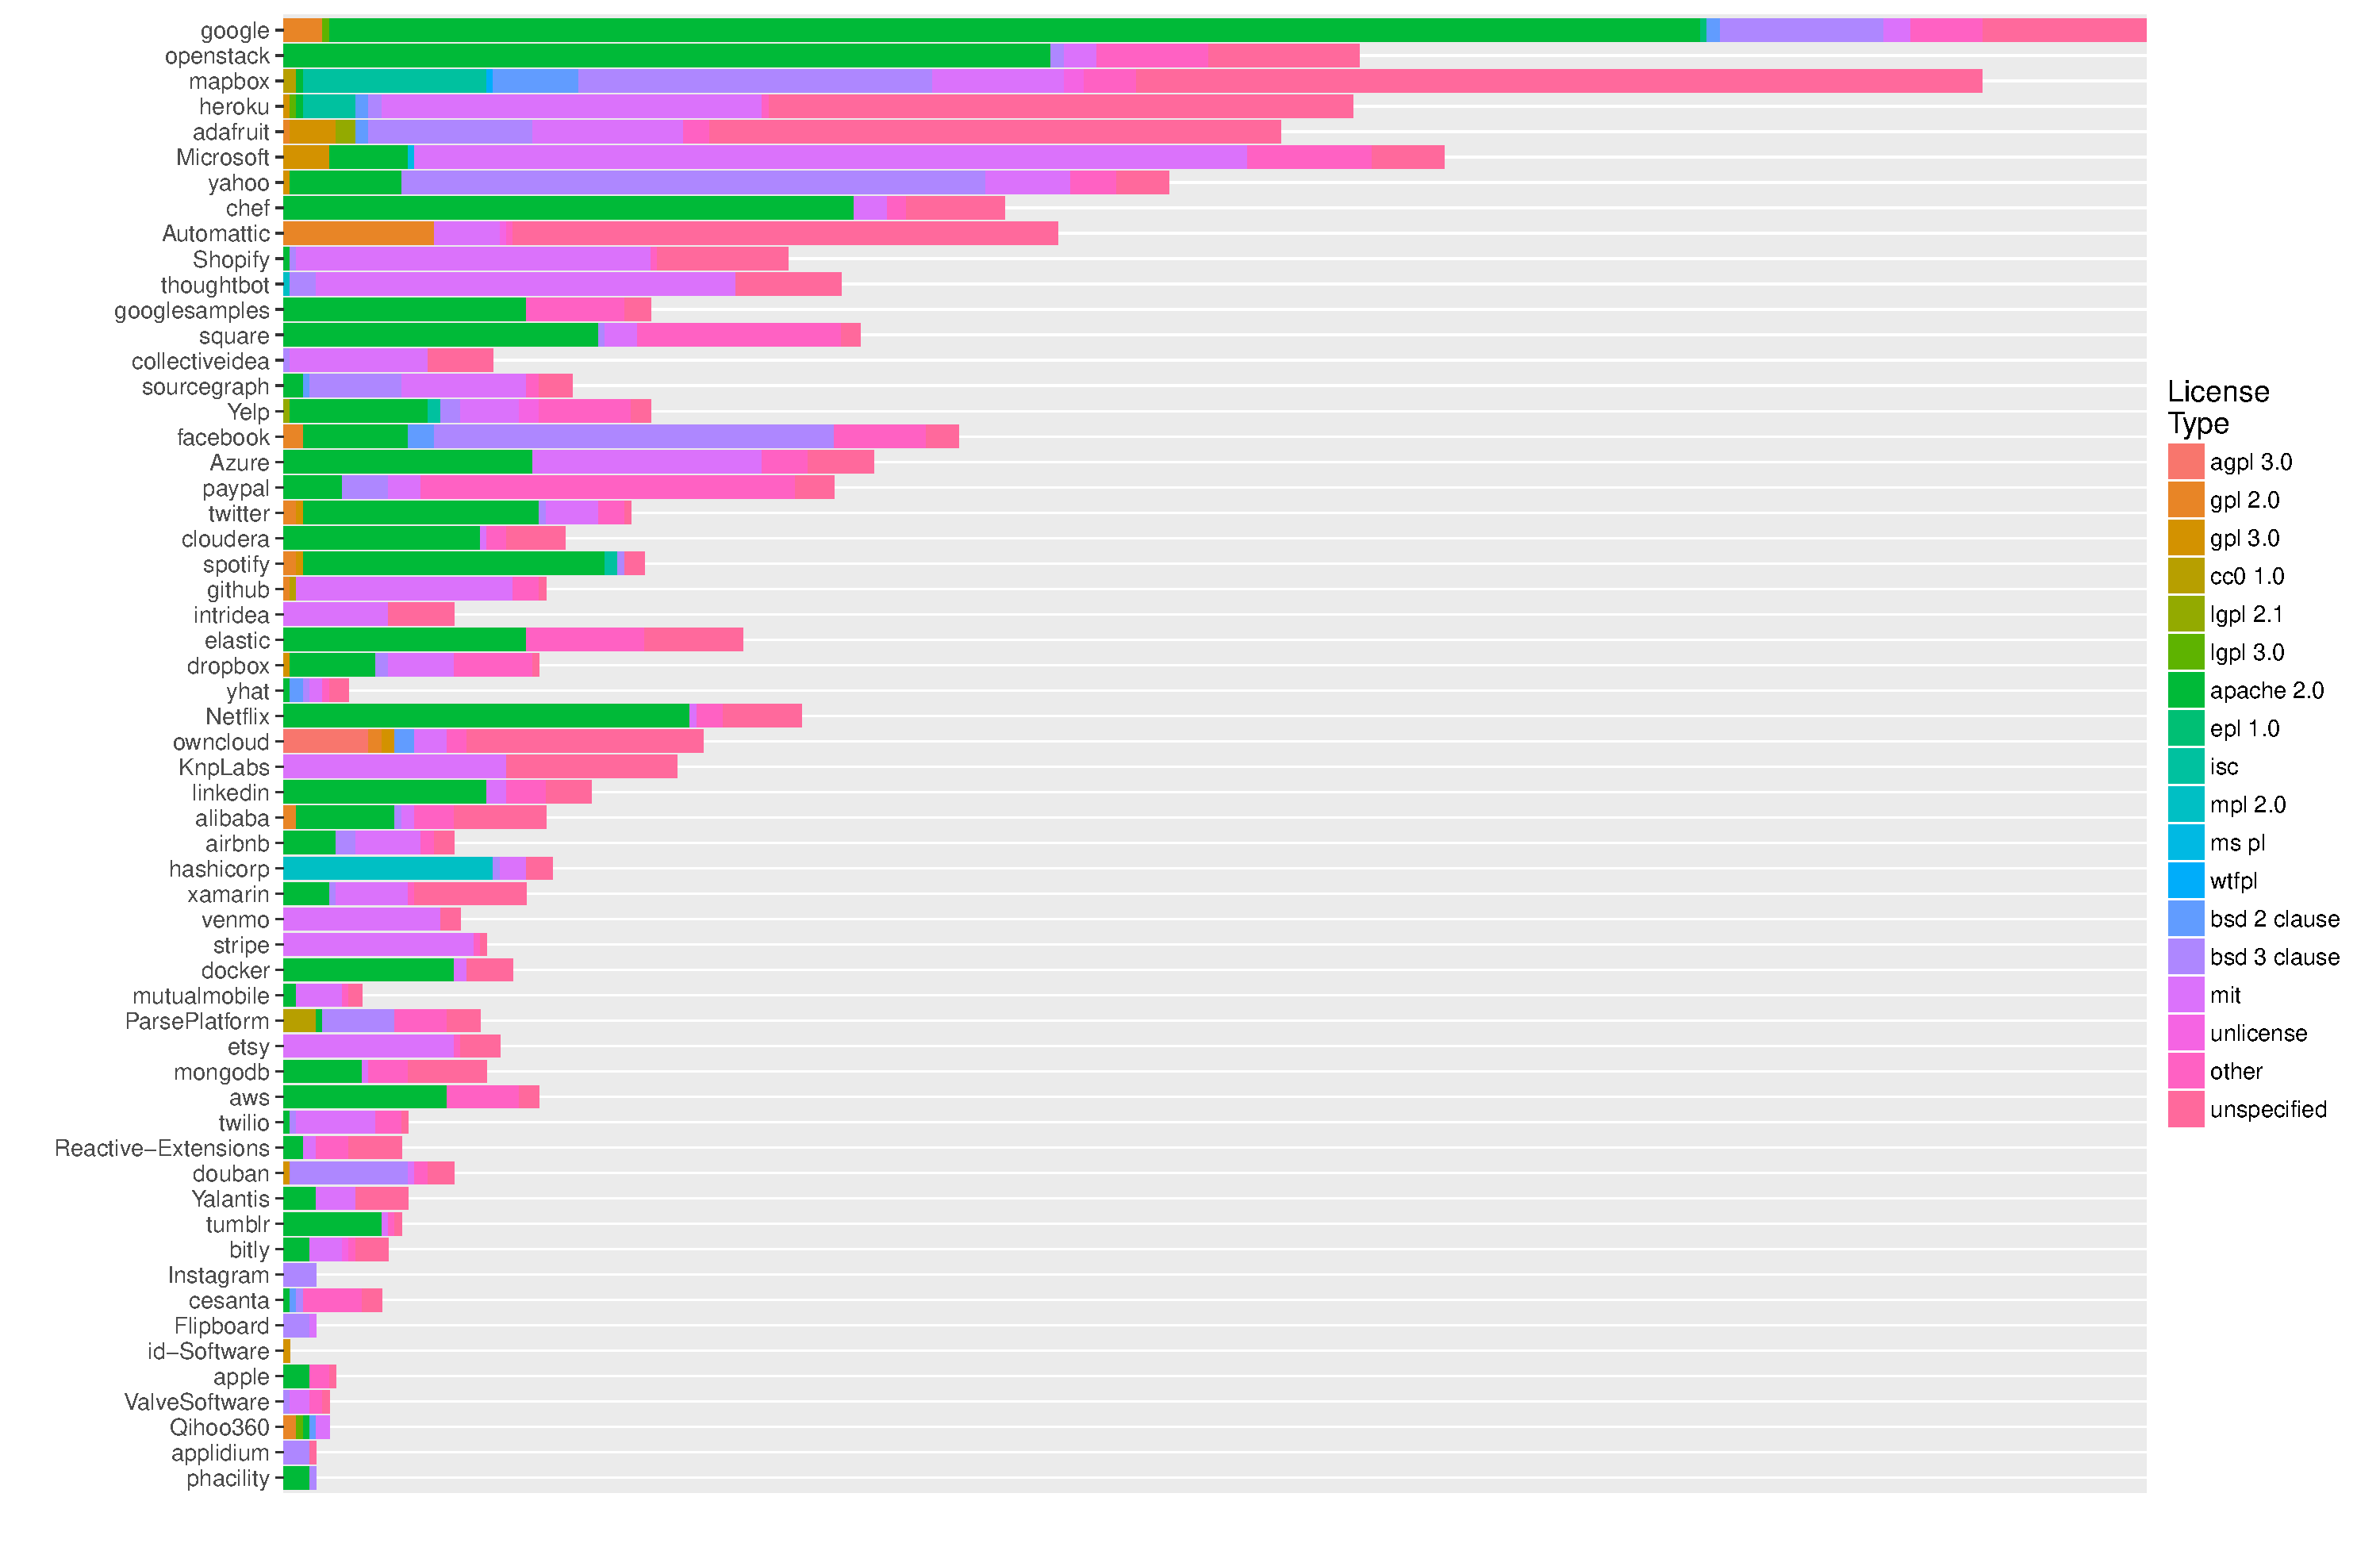
\includegraphics[page=1,scale=0.3]{../graphics/intro/which_firm_is_using_which_license.pdf}
	\caption{Most OS projects by firms do use (very) permissive licenses (from green over blue to magenta). The x-axis (caption not in the plot) represents the absolute number of repositories (from 15 - 284 repositories).}
	\label{fig:licenses_used_by_firms}
\end{figure}

\begin{figure}[!h]
	\centering
	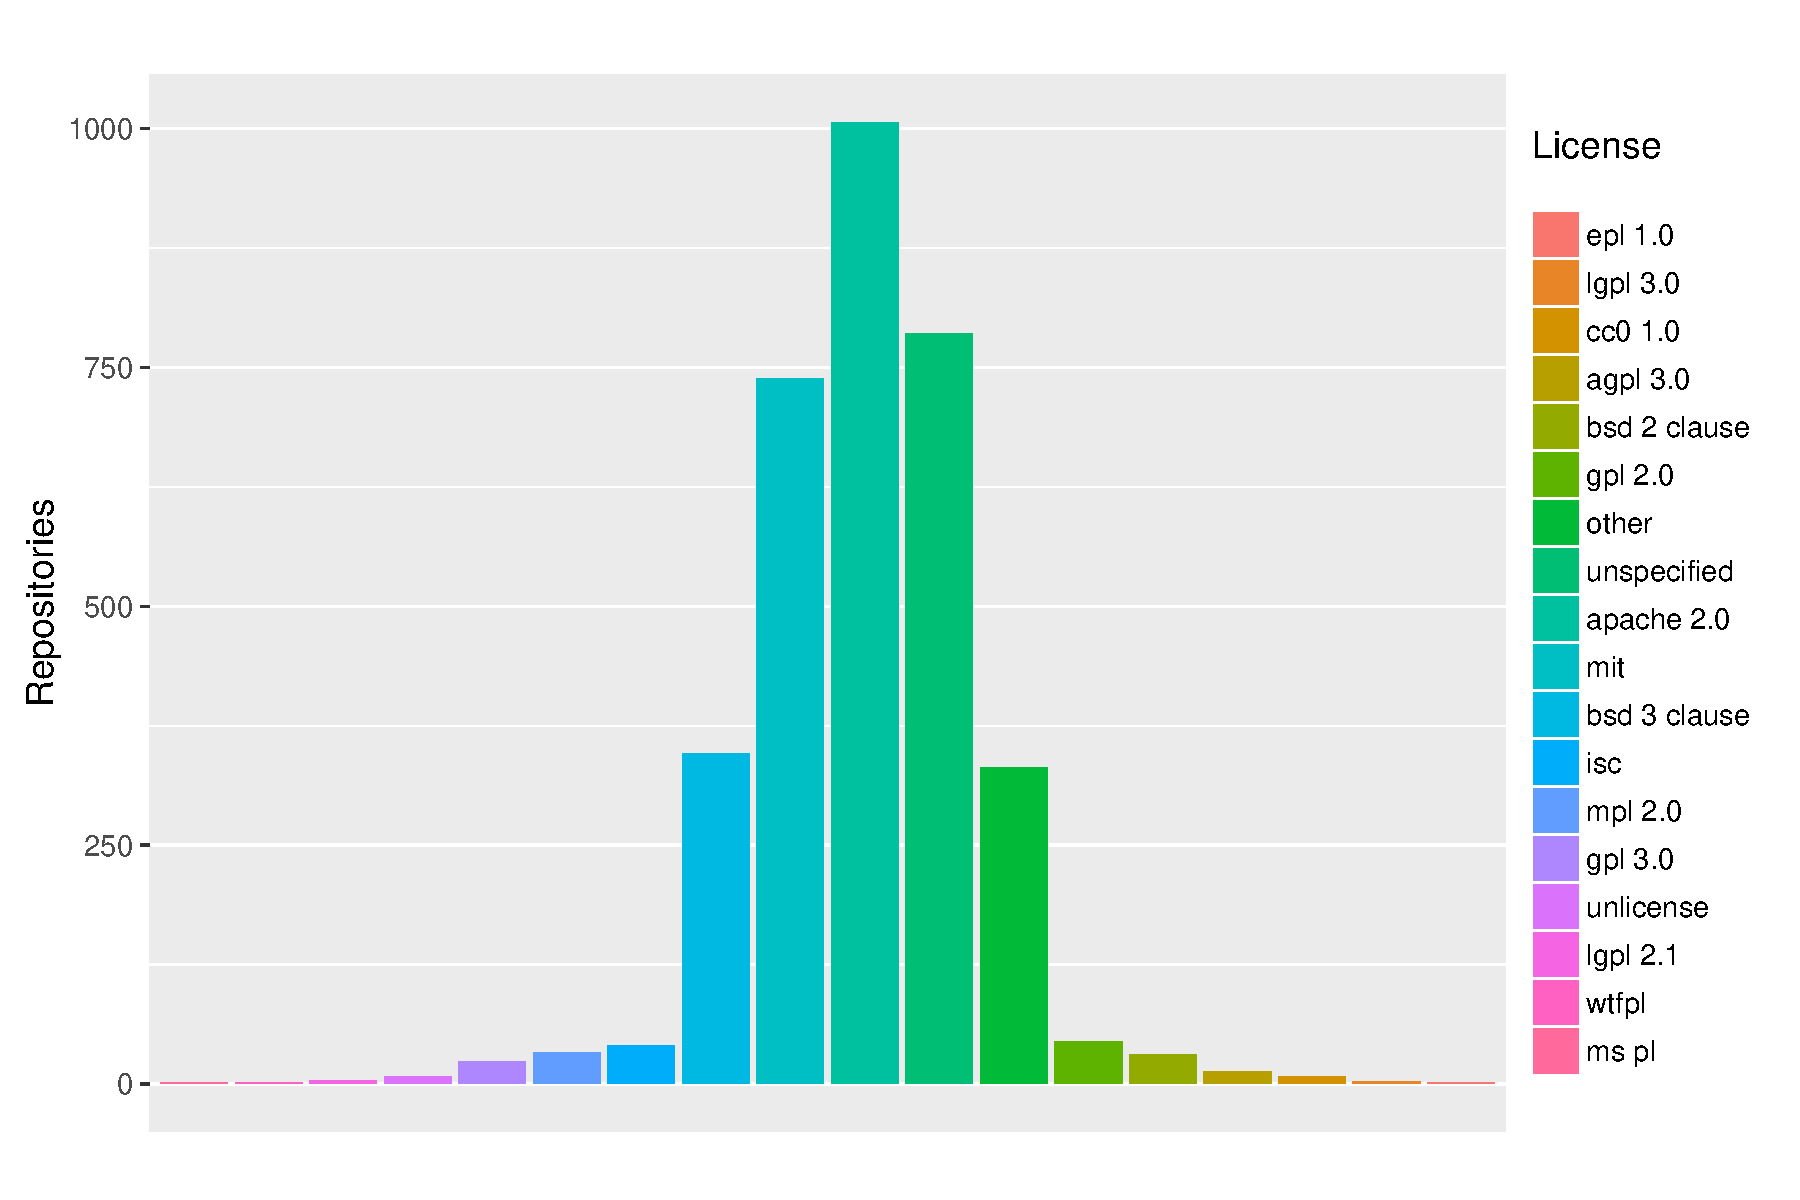
\includegraphics[page=1,scale=0.4]{../graphics/intro/licenses/popular_licenses.pdf}
	\caption{Frequency of licenses in GitHub repositories of firms. Permissive licenses (like Apache, MIT and BSD) are favored. \textit{Unspecified} means not categorized (i.e. in most cases proprietary OS license by firm). Graphs for Top and Residual Projects in figure \ref{fig:licenses_in_residual_projects} and \ref{fig:licenses_in_top_projects}.}
	\label{fig:licenses_in_projects}
\end{figure}

\clearpage
\textbf{Strong Copyleft (restrictive)}

\begin{itemize}
	\item GNU Affero General Public License (agpl 3.0)
	\item GNU General Public License (gpl 2.0, gpl 3.0)
	\item Creative Commons CC0 1.0 Universal (cc0 1.0)
	\item SIL Open Font License (ofl 1.1)
\end{itemize}

\textbf{Mixed (less restrictive, more permissive)}

\begin{itemize}
	\item GNU Lesser General Public License, Version 2.1 (lgpl 2.1, lgpl 3.0)
	\item Apache License, Version 2.0 (apache 2.0)
	\item Eclipse Public License (epl 1.0)
	\item ISC-Licence (isc)
	\item Mozilla Public License, version 2.0 (mpl 2.0)
	\item Microsoft Public License (ms pl)
\end{itemize}


\textbf{Non-Copyleft (very permissive)}

\begin{itemize}
	\item Do What The Fuck You Want To Public License (wtfpl)
	\item BSD licenses (bsd 2 clause, bsd 3 clause)
	\item The MIT License (mit)
\end{itemize}

\textbf{Uncategorized}

Beside that there are also unlicensed projects (i.e. no license on "purpose") and license unspecified projects (i.e. no license detected by GitHub).

\subsection{Classification of Developers}

We distinguish two groups of participants:

\begin{enumerate}
	\item [\textbf{1) Internal Developers}] (also called \textit{firm employed developers}) are developers / users who
	\begin{itemize}
		\item are currently employed at the company of the observed project, or
		\item were employed at the company of the observed project in the past
	\end{itemize}
	\item [\textbf{2) External Developers}] are developers / users who
	\begin{itemize}
		\item never worked at the company of the observed project, and / or
		\item are independent developers / hobbyist programmer
	\end{itemize}
\end{enumerate}

\subsection{Evaluation and Classification of Commits}

A \textit{commit} represents the participation of a developer. It includes code changes or new code \footnote{detailed code changes can be inspected by \textit{git diff \$commithash}}. In the following, we will regard a commit as a participation activity. We ignore the size of the commit (how many lines and files have changed) because measuring code quality by these simple metrics would be difficult. According to \cite{stamelos2002code} further specialized software is needed to measure code quality reliable.

The number of projects' valid commits of the selected 58 firms is 2,951,188. These commits are used in the final version of the projects (i.e. they are productive code commits). Commits without a valid email address \footnote{here a valid email address following ABNF with the regular expression
\tiny{\verbatiminput{../listings/w3c_html5_email.regex}}
Source: \url{http://www.w3.org/TR/html5/forms.html\#valid-e-mail-address}
} are sorted out. As mentioned before, a commit can also be a \textbf{merge} and is taken into account as well \footnote{\textit{Merge} is an activity of implementing proposed code changes into the (final) project}.

There are 1,111,384 of firm employed developers and 1,839,804 of external developers \footnote{for classification see next section}. Thus, the share of firm employed developers is at least 37.66 \% on all observed projects.

To compare the participation of firm employed and not firm employed developers, each commit must be identified by the author's email address and be assigned to internal (i.e. employed by firm) or external (i.e. employed not by firm of the project). The selection of firm employed developers is quite conservative, because we only regard developers with a firm e-mail address or developers which are known to work for the company. Many more developers may work or have been working for the firm in the past.

To maximize the classification of firm employed developers with acceptable effort, a whitelist was generated and checked manually via LinkedIn for the developers with the highest share of participation. The whitelist \footnote{can be received as csv file: \url{https://git.zeitpulse.com/philipp/masterthesis-data/raw/master/csv/classification/int_ext_developer_classification.csv}} contains over 550 manually checked developers, everyone with a share of code contribution from 25 \% up to  100 \% for a specific project.

\subsection{Time and Location of Code Contribution}

Through almost 3 Mio. observed commits we can measure a representative frequency of code contribution (see figures \ref{fig:distribution_developer_commits_by_timezone}, \ref{fig:distribution_developer_commits_local}, \ref{fig:distribution_developer_commits_wordlwide} and \ref{fig:distribution_developer_commits_by_month}). The histograms are stacked and not overlaid \footnote{the total number of commits by not firm employees is actually higher (see previous section for numbers)}.

\textbf{Interpretation}: Most of the code contribution takes place between 9:00 and 19:00 with its peak at 15:00 (see table \ref{fig:distribution_developer_commits_local}). An interesing observation is that firm employed developers' and external developers' code contributions frequency is very similar. The reasons could be:

\begin{enumerate}[a)]
	\item external developers are employed as well (but at another firm)
	\item externals / freelance workers write and commit code in the same time frame because they are most efficient in that time frame
	\item externals / freelance workers write and commit code in the same time frame because code contribution is a form of collaboration and "forces" same time frames
\end{enumerate}

According to the manual classification of developers (most of them are or were employed at the particular firm) and the fact that code contribution time is similar regarding to the local time, reason a) seems to be the prime cause: \textbf{external developers are employed developers of other / rival firms}.

Beside that, the core hours are in line with independent studies about working hours (see figure \ref{fig:us_standard_workday}). Thus, the most effective time period for developers seems to be between midday and late afternoon. The distribution of worldwide code contribution confirms the leading role of Silicon Valley / California / Oregon and USA in the firm managed open source segment (see figure \ref{fig:distribution_developer_commits_by_timezone} and  \ref{fig:distribution_developer_commits_wordlwide})

\begin{figure}[!ht]
	\centering
	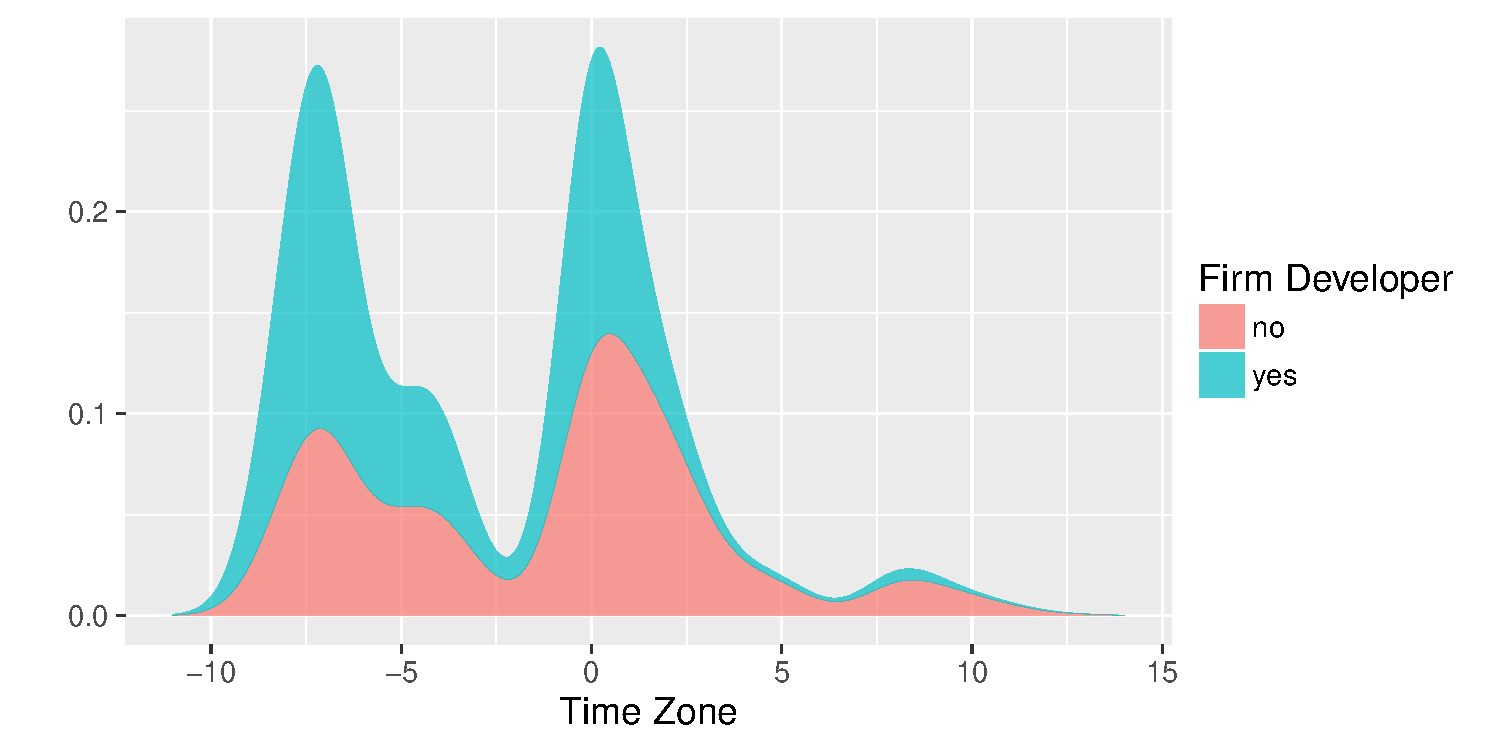
\includegraphics[page=1,scale=0.7]{../graphics/intro/timezone_of_code_contribution.pdf}
	\caption{Code contributions by firm employed and external developers over time zones. Assumption: Most code contributions are from Europe (UTC between -1 and +2) and USA / Canada (UTC between -4 and -8) by considering economicaly most successful countries by longitude (and ignoring latitude influences).}
	\label{fig:distribution_developer_commits_by_timezone}
\end{figure}

\begin{figure}[!ht]
	\centering
	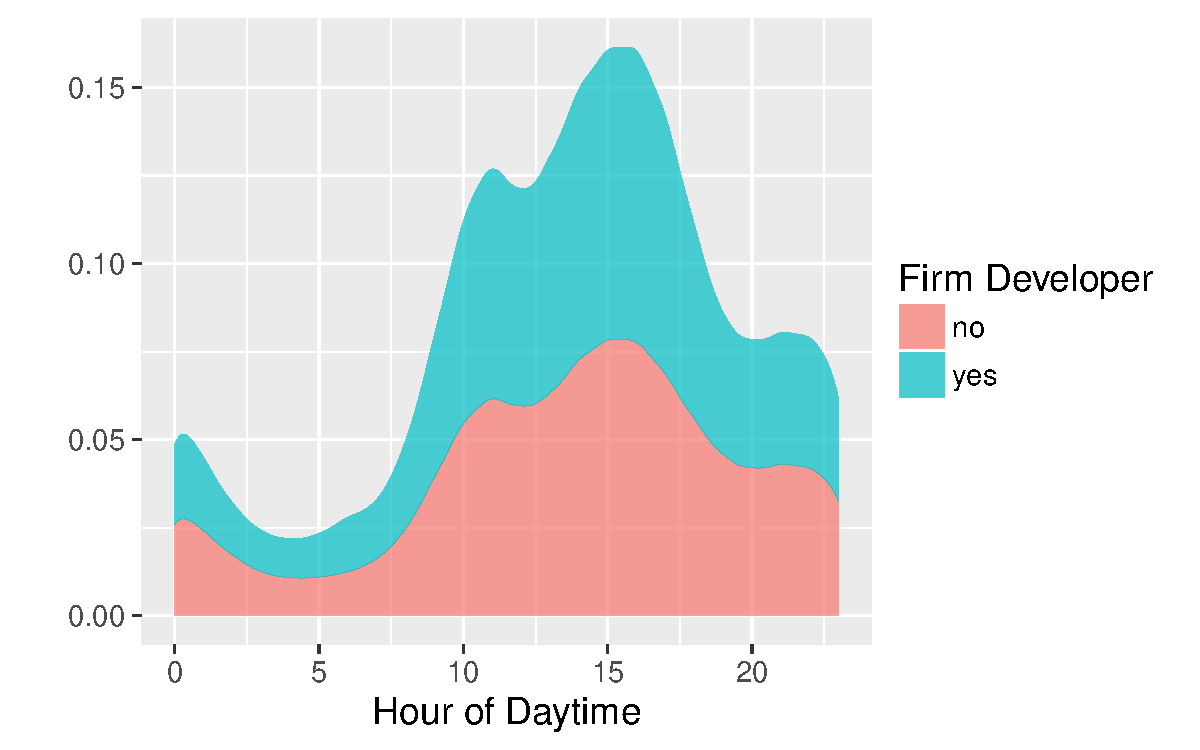
\includegraphics[page=1,scale=0.7]{../graphics/intro/hour_of_code_contribution_daytime_local.pdf}
	\caption{Code contributions of firm employed and external developers by local daytime (workdays, weekend and holidays are included). Most of the code commits are placed between 09:00 - 19:00, with its peak between 15:00 - 16:00}
	\label{fig:distribution_developer_commits_local}
\end{figure}

\begin{figure}[!ht]
	\centering
	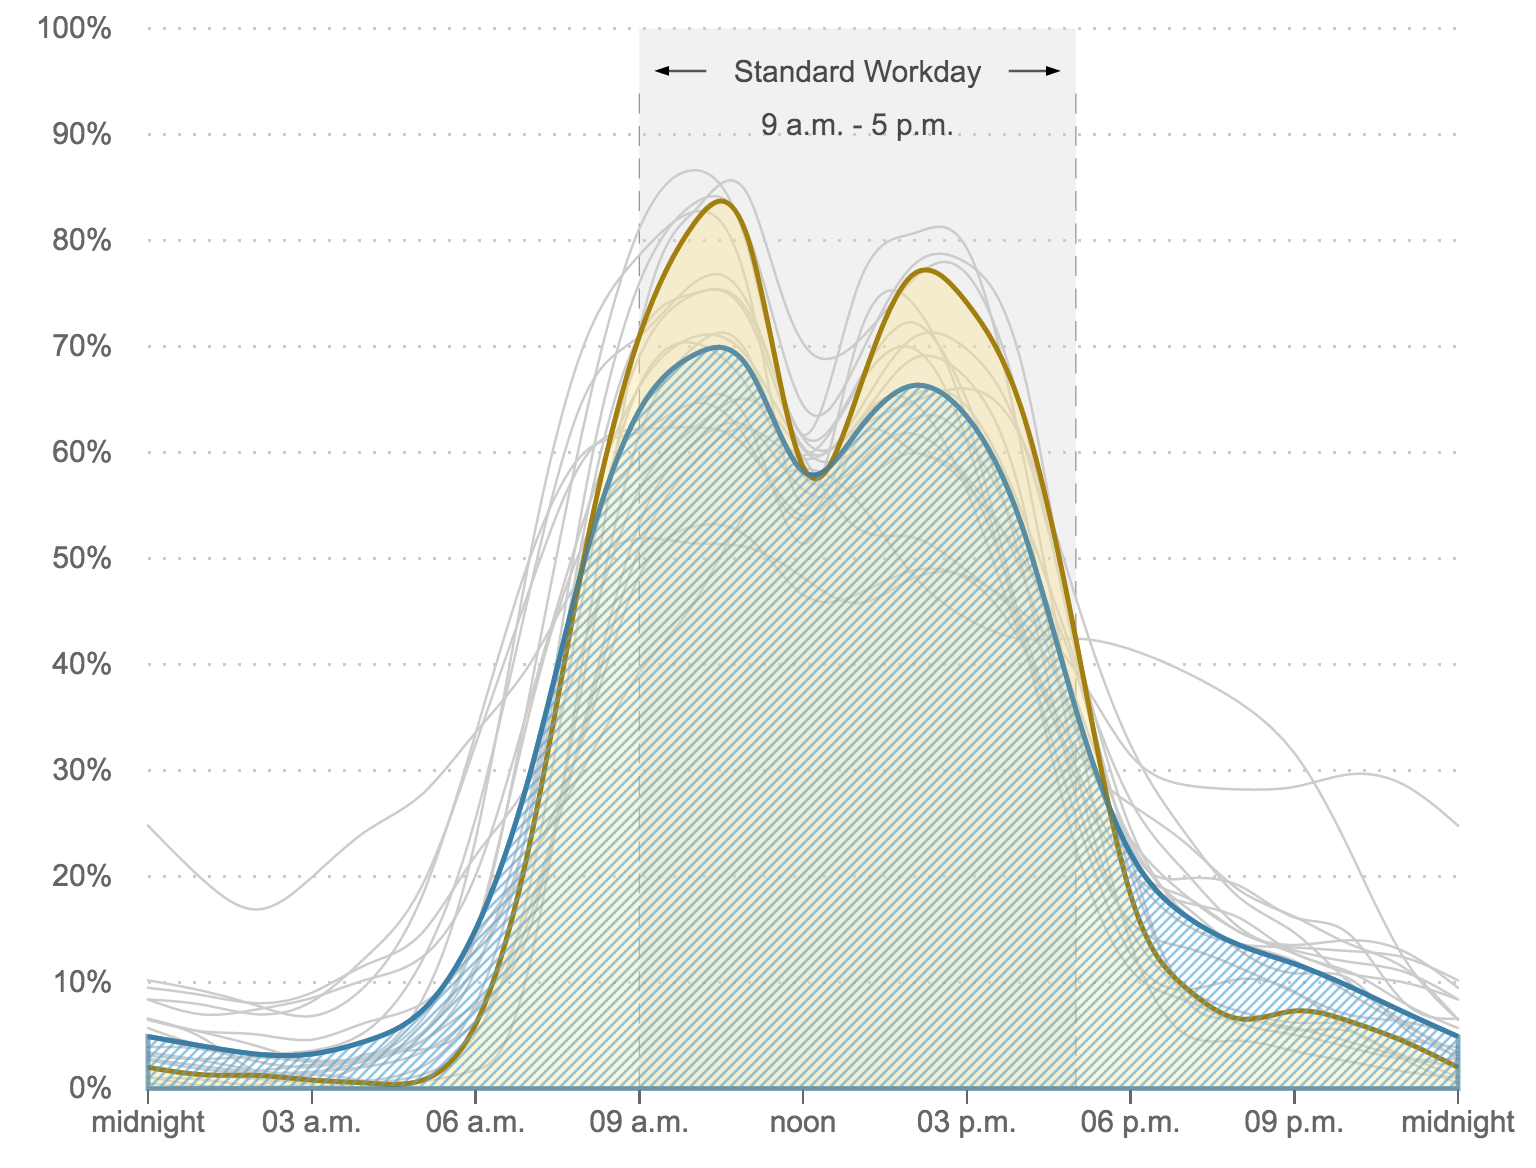
\includegraphics[scale=0.4]{../graphics/images/us_standard_workday.png}
	\caption{2011-2012 Annual Averages ("Computer and Mathematical" (yellow) compared to "All Jobs" (green)): \textit{The majority of people are at work from 9:00 to 17:00, with a small break in the middle of the day for lunch} (according to \cite{TheAmericanWorkdayInOneGraph:online}). \footnotesize{Source: BLS, American Time Use Survey; Credit: Quoctrung Bui/NPR}}
	\label{fig:us_standard_workday}
\end{figure}

\clearpage
\subsection{Observed Repositories}

The final number of observed repositories is 3,419, including 610 top projects and 2,809 residual projects (see table \ref{tbl:overviewrepositories} for further details).

\begin{table}[!ht] \centering
	\footnotesize
	
% Table created by stargazer v.5.2 by Marek Hlavac, Harvard University. E-mail: hlavac at fas.harvard.edu
% Date and time: Sat, Mar 12, 2016 - 20:59:40

\begin{tabular}{@{\extracolsep{5pt}}lccccc}
\\[-1.8ex]\hline
\hline \\[-1.8ex]
Statistic & \multicolumn{1}{c}{N} & \multicolumn{1}{c}{Mean} & \multicolumn{1}{c}{St. Dev.} & \multicolumn{1}{c}{Min} & \multicolumn{1}{c}{Max} \\
\hline \\[-1.8ex]
Age (in days) & 3,419 & 743.790 & 560.458 & 0 & 2,904 \\
Number of Contributors & 3,419 & 17.181 & 40.053 & 2 & 468 \\
Number of Commits & 3,419 & 748.581 & 8,510.597 & 2 & 428,840 \\
Number of Commits by firm employed developers & 3,419 & 250.875 & 1,501.224 & 0 & 56,624 \\
All Issues count & 3,419 & 20.836 & 75.842 & 1 & 1,884 \\
Closed Issues count & 3,419 & 2.817 & 18.725 & 0 & 706 \\
Open Issues count & 3,419 & 18.019 & 74.182 & 0 & 1,884 \\
Stars & 3,419 & 426.290 & 1,538.234 & 0 & 35,214 \\
Subscribers & 3,419 & 75.221 & 123.100 & 1 & 2,617 \\
Forks & 3,419 & 99.204 & 378.507 & 0 & 10,772 \\
Ratio (share of firm employed developers) & 3,419 & 0.521 & 0.348 & 0.000 & 1.000 \\
Mean share of Top Repositories & 3,419 & 0.178 & 0.383 & 0 & 1 \\
\hline \\[-1.8ex]
\end{tabular}
% \end{table}

	\caption{Statistic of observed GitHub Projects}
  \label{tbl:overviewrepositories}
\end{table}

The number of repositories (i.e. observations) will vary between statistical models \footnote{some are using "Top Repositories", "Residual Repositories", "All Repositories" and "Repositories older than X days" for instance}.

\subsection{The Role of Developers on Issues}

\textit{Issues} are communication channels for GitHub repositories. GitHub provides data of users who opened issues and users who participate on issues by commenting / discussing. All comments will be counted and assigned to firm employed and external developers \footnote{some models also include a measurement of weighted comments by its content size}.

As mentioned before, issues can:

\begin{itemize}
	\item be technical (bug reports / source code related)
	\item include general ideas / feature requests
	\item be organizational related
\end{itemize}

Finally, we have 405,163 issues with 1,718,363 comments (6,190 issues and 32,599 issues' comments are by firm employed developers).

\subsection{Firms' OS Commitment as Proxy for Quality of Work Environment}

\label{sec:glassdoor_ratings}

To which extend does contribution of firm employees on firms' OS projects reflect the employer quality? If employed developers get encouraged by their employer to initiated and contribute on OS project, do they stay more likely at their current employer or rate their working climate more positive? If an firm employed developer is allowed to work on OS projects as part of his work, does it increase their incentive to be more creative and try out new ideas by themselves? Or do developers initiate projects to demonstrate and promote a specific technology innovation inside a firm?

This research question itself would probably fill another study (see \ref{sec:further_research}). But we will observe briefly a few data collections regarding to work climate and GitHub activities of firms. For that, ratings from employees of their workplace are evaluated. The data is received from Glassdoor. Ratings of 50 firms were found \footnote{\url{https://git.zeitpulse.com/philipp/masterthesis-data/tree/master/apidata/glassdoor/employers}} but only 14 firms (see table \ref{tbl:glassdoor_firm_ratings}) had enough ratings and enough Top Repositories (i.e. at least 38 ratings and 10 Top Repositories) to be "representative" with partly significant regression results. However, there is a (weak) positive significant relation between the number of popular OS projects and the rating by the employees (and vice versa) which could be measured by \textit{employees rating their firm} and \textit{firms' number of popular Open Source projects on GitHub} through the OLS method (see table \ref{tbl:glassdoorfirmratingandosprojects} for details). Interpretation: (a) if a firm initiates more OS projects, the firm is more valuable as employer for developers (b) if a firm is a good place to work, employees will more likely initiate OS projects through the firm.

Thus, the numbers of observations / ratings are not representative and might be a promising approach for further research.

\begin{table}[!h] \centering
	\scriptsize{
	
% Table created by stargazer v.5.2 by Marek Hlavac, Harvard University. E-mail: hlavac at fas.harvard.edu
% Date and time: Mi, Feb 10, 2016 - 20:05:53
\begin{tabular}{@{\extracolsep{5pt}}lcccc}
\\[-1.8ex]\hline
\hline \\[-1.8ex]
 & \multicolumn{4}{c}{\textit{Dependent variable:}} \\
\cline{2-5}
\\[-1.8ex] & Rating & OS Projects & Ratings count & Work-Life-Balance \\
\\[-1.8ex] & (1) & (2) & (3) & (4)\\
\hline \\[-1.8ex]
 Average Ratio Top Projects & $-$0.115 & 12.263 & 4,441.273 & 0.222 \\
  & (0.226) & (21.167) & (5,659.478) & (0.446) \\
  & & & & \\
 Average Ratio Residual Projects & 0.108 & $-$21.155 & $-$386.364 & $-$0.342 \\
  & (0.217) & (18.723) & (5,751.773) & (0.410) \\
  & & & & \\
 Ratings Count & 0.00003$^{*}$ & $-$0.002 &  & $-$0.00004 \\
  & (0.00001) & (0.001) &  & (0.00003) \\
  & & & & \\
 Rating &  & 74.312$^{**}$ & 17,654.490$^{*}$ & 1.638$^{**}$ \\
  &  & (25.873) & (8,434.416) & (0.486) \\
  & & & & \\
 Culture and Values & 0.634$^{***}$ & $-$37.375 & $-$13,061.970$^{*}$ & $-$0.769 \\
  & (0.132) & (24.268) & (5,587.065) & (0.510) \\
  & & & & \\
 Work-Life-Balance & 0.424$^{**}$ & $-$42.472$^{***}$ & $-$7,375.867 &  \\
  & (0.126) & (9.910) & (4,863.693) &  \\
  & & & & \\
 Age of Firm on GitHub & $-$0.0001 & 0.014$^{**}$ & 0.728 & 0.0003$^{**}$ \\
  & (0.0001) & (0.004) & (2.016) & (0.0001) \\
  & & & & \\
 OS Projects count & 0.008$^{**}$ &  & $-$142.543 & $-$0.019$^{***}$ \\
  & (0.003) &  & (104.811) & (0.004) \\
  & & & & \\
 Residual Repos. count & $-$0.001$^{**}$ & 0.152$^{***}$ & 26.620 & 0.003$^{***}$ \\
  & (0.0005) & (0.018) & (15.218) & (0.001) \\
  & & & & \\
 Constant & 0.024 & $-$4.067 & 7,961.749 & $-$0.065 \\
  & (0.338) & (31.831) & (7,988.258) & (0.665) \\
  & & & & \\
\hline \\[-1.8ex]
Observations & 14 & 14 & 14 & 14 \\
R$^{2}$ & 0.985 & 0.957 & 0.891 & 0.955 \\
Adjusted R$^{2}$ & 0.962 & 0.889 & 0.718 & 0.884 \\
Residual Std. Error (df = 5) & 0.076 & 7.202 & 1,975.574 & 0.150 \\
F Statistic (df = 8; 5) & 41.895$^{***}$ & 14.067$^{***}$ & 5.135$^{**}$ & 13.407$^{***}$ \\
\hline
\hline \\[-1.8ex]
\textit{Note:}  & \multicolumn{4}{r}{$^{*}$p$<$0.1; $^{**}$p$<$0.05; $^{***}$p$<$0.01} \\
\end{tabular}

	}
	\caption{Rating of Work Environment by employees and Firms' activity on Open Source projects}
  \label{tbl:glassdoorfirmratingandosprojects}
\end{table}

\clearpage

\subsection{Microsoft and GitHub Inc.: Contribution and Social Success Metrics of Atom and VSC}
\label{sec:atom_vs_vsc}

\begin{table}[!h]
\footnotesize{
\centering
\begin{tabular}{rllllllrllll}
  \hline
 & Init. by Firm & Editor & License & Stars & Subscr. & Forks & Contrib. & Published & Op.Issues & Commits & Ratio \\
  \hline
1 & GitHub & Atom & MIT & 23,998 & 1,524 & 4,094 & 260 & 2014 Q2 & 1,644 & 27,373 & 73.63\% \\
  2 & Microsoft & VSC & MIT & 9,884 & 679 & 1,205 &  56 & 2015 Q2 & 774 & 1,909 & 58.87\% \\
   \hline
\end{tabular}
\label{tbl:dataofvscodeandatom}
\caption[Repository Data of Atom and VSC]{Repository Data of Atom and VSC \protect\footnotemark}
}
\end{table}
\footnotetext{\ \ Retrieved on: \nth{21} January 2016 via \url{https://github.com/}}

The time series \ref{fig:codecontributionatomeditor} and \ref{fig:codecontributionvsc} \footnote{Retrieved on \nth{18} January 2016 via 'git log'} show the code contribution of \textit{GitHub} / \textit{Microsoft} employed developers against \textit{external developers}. \textbf{Gold} represents code contribution by external developers, \textbf{Black} represents code contribution by firm employed developers. \textit{Atom} was published as open source in May 2015, \textit{VSC} a half year later in November 2015.

If you compare the basic statistics of the competitors \textit{Microsoft} and \textit{GitHub Inc.} (see table \ref{tbl:summary_microsoft} and \ref{tbl:summary_github} on page \pageref{tbl:summary_microsoft}) you can see that \textit{Microsoft} is a "youngster" on \textit{GitHub} \footnote{the following values are mean values of each firms' projects}: Microsoft projects have a mean age of less than 1 year, high share of firm employed developers (over 68 \%) and fewer "Top Projects" (18 \% of Microsofts' projects are "Top Projects"). Whereas \textit{GitHub Inc.'s} "Top Project" share is 40 \% with a lower share of firm employed developers (53 \%) and older projects (mean age is almost 2 years).

\textbf{Interpretation:} This basic statistic provides indications of the differences between the two companies \textit{GitHub Inc.} and \textit{Microsoft}: Microsoft is a "newer" member of the OS community (according to the age of projects) and tries to gain its reputation (by initial high share of firm employed developers) and tries to establish popular projects (share of "Top Projects") with the long-range objective to motivate external developers (i.e. the OS community) to participate on their projects.

\begin{figure}[!h]
	\centering
	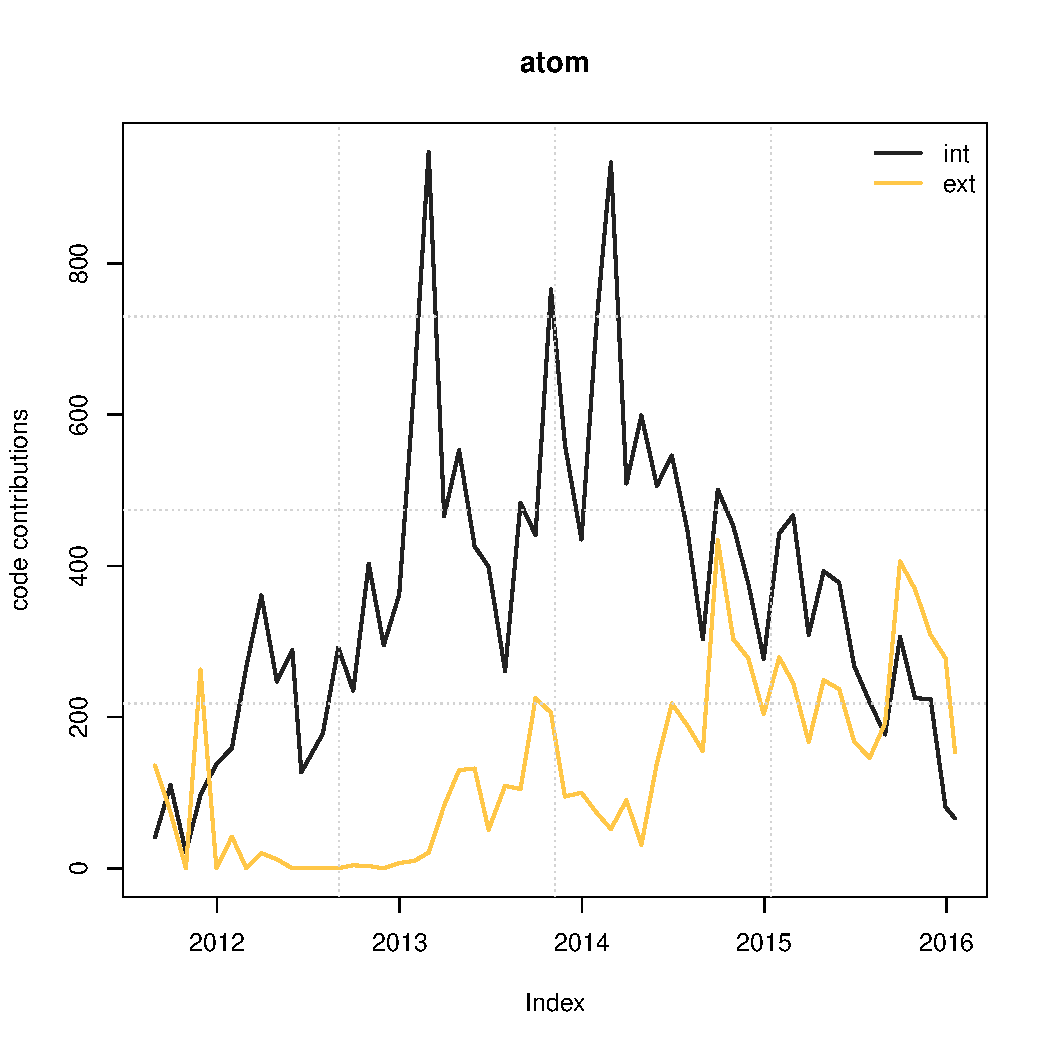
\includegraphics[page=1,scale=0.5]{../graphics/plots/timeseries/atom_vs_vscode/timeseries_repos_atom.pdf}
	\caption{Code Contribution of "Firm employed Developers" (int) and "External Developers" (ext) to Atom (GitHub Inc.). Published as open source in May 2015}
	\label{fig:codecontributionatomeditor}
\end{figure}

\begin{figure}[!h]
	\centering
	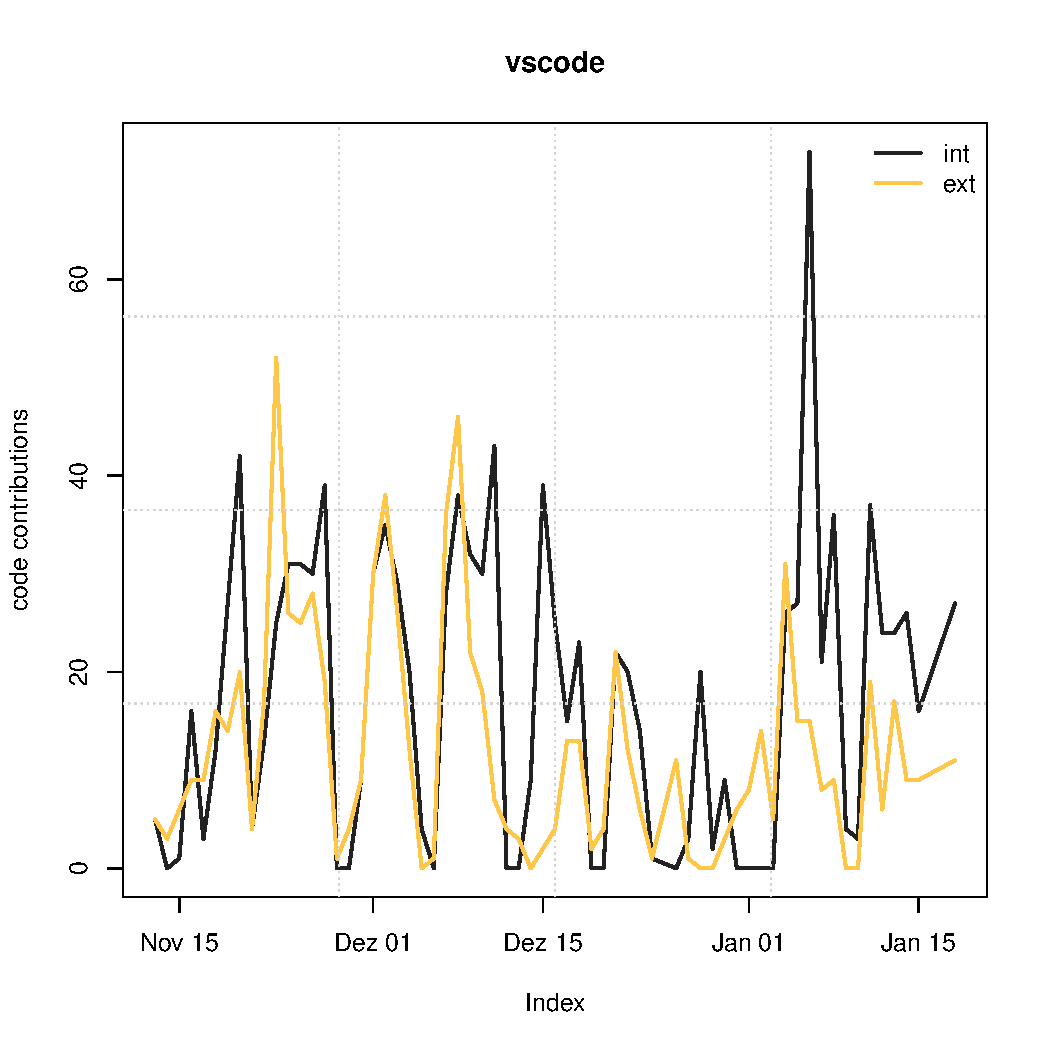
\includegraphics[page=1,scale=0.5]{../graphics/plots/timeseries/atom_vs_vscode/timeseries_repos_vscode.pdf}
	\caption{Code Contribution of "Firm employed Developers" (int) and "External Developers" to Visual Studio Code (Microsoft). Published as open source in November 2015. (time range of plot: Nov. 2015 - Jan. 2016)}
	\label{fig:codecontributionvsc}
\end{figure}


\newpage
%\addcontentsline{toc}{section}{Hypotheses}
\clearpage
\section{Analysis}
\label{sec:empirical_findings}

With the information of code commits, \textit{GitHub} projects' metrics, issue communication and user events (over time) we can verify the following hypotheses:

\begin{itemize}
    \item [\textbf{H 1}] Firm employees' participation affects the participation of external developers
		\begin{itemize}
			\item [\textbf{H 1.1}] If firm employees contribute source code more often, external developers do as well
			\item [\textbf{H 1.2}] If firm employees participate more often on issue threads, external developers do as well
		\end{itemize}
    \item [\textbf{H 2}] Firm employees' participation (in the beginning) affects the (later) success of firm-initiated open source projects
		\begin{itemize}
			\item [\textbf{H 2.1}] If firm employees contribute source code more often in the beginning, the project gets more successful
		\end{itemize}
		\item [\textbf{H 3}] If firm employees' contribution share is higher overall the more likely the project is popular
\end{itemize}


\subsection{Terms and Definitions}
\label{sec:lm_terms_and_definitions}
\begin{itemize}
	\item [\textbf{Younger Projects:}] Projects that are younger than 1 year (\textless 365 days)
	\item [\textbf{Older Projects:}] Projects that are older than 1 year (\textgreater= 365 days)
	\item [\textbf{Top Projects:}] Projects that were found in the first 1000 most popular projects of a programming language (can be 1 or 0, see below for mathematical definition)
	\item [\textbf{Residual Projects}] Projects that were \textit{not} found in the 1000 most popular projects for a programming language \footnote{"Top Projects" and "Residual Projects" together build the set of relevant projects}
	\item [\textbf{Ratio}] Code commit share of firm employed developers to external developers (normalized value between 0 and 1)
\end{itemize}

\begin{align}
\mathit{Ratio} =
	\begin{cases}
		1         & \quad \text{if repository is maintained to 100\% by firm employed developers only}\\
		0         & \quad \text{if repository is maintained to 0\% by firm developers (i.e. 100\% external developers)}\\
		\in (0,1) & \quad \text{else}\\
	\end{cases}
\end{align}

\begin{align}
\mathit{Top \ Project} =
	\begin{cases}
		1         & \quad \text{if is found in search of 1000 most starred projects of the 10 selected Languages}\\
		0         & \quad \text{else}\\
	\end{cases}
\end{align}

\subsection{Slopes and Dots (on plot figures)}
\label{sec:lm_plots_description}
\begin{itemize}
	\item [\textbf{Yellow-Solid}]
	$\vcenter{\hbox{
\includegraphics[scale=0.05]{../hypotheses/legend/yellow_slope.png}}}$
	Correlation coefficient for the influence of code commits from firm employed developers on external developers (via OLS)

	\item [\textbf{Blue-Dashed}]
	$\vcenter{\hbox{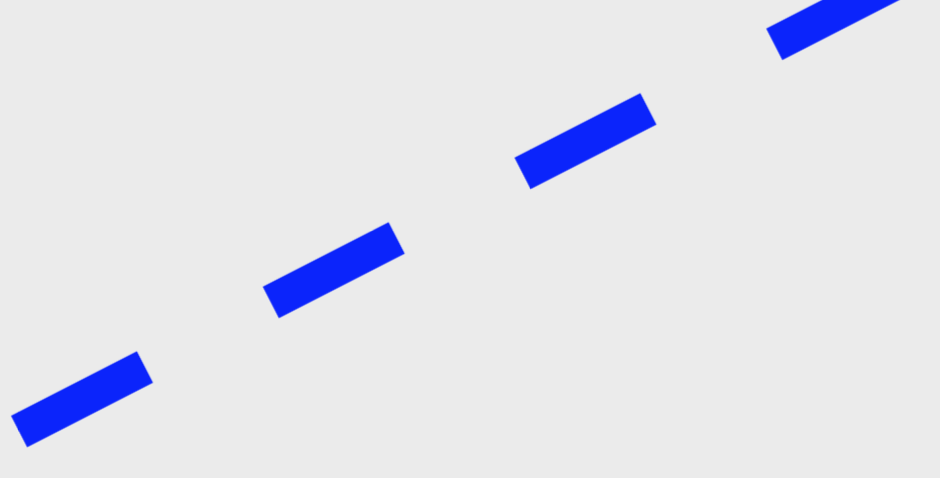
\includegraphics[scale=0.045]{../hypotheses/legend/blue_slope.png}}}$
	Correlation coefficient for the influence of code commits from external developers on firm employed developers (via OLS) \footnote{actually x- and y-axis must be reverted to illustrate external impact on firm employed developers, but for the sake of simplicity blue and yellow slopes share one plot here}

	\item [\textbf{Grey Dots}] $\vcenter{\hbox{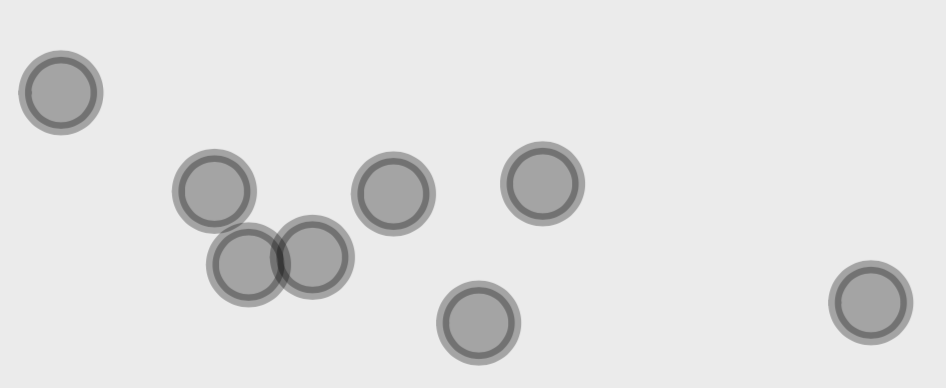
\includegraphics[scale=0.07]{../hypotheses/legend/dots.png}}}$
	Number of code contribution by firm employed developers (x-axis) and external developers (y-axis)

\end{itemize}

\subsection{H 1: Firm employees' participation affects the participation of external developers}
\subsection{H 1.1: If firm employees contribute source code more often, external developers do as well}

\subsubsection{H 1.1: Models and Terminology}

The following linear models (using OLS) examine the influence of code contribution by firm employed developers on external developers and vice versa.

Every project is represented by a dot and plotted through number of code contributions by firm employed developers (x-axis) against number of code contributions by external developers (y-axis). The influence of firm employed developers' participation (independent) on external developers' participation (dependent) is represented by the solid yellow slope and defined in the models 1.1, 1.3, 1.5, 1.7, 1.9, 1.11 and 1.13. Conversely, the influence of external developers' participation (independent) on firm employed developers' participation (dependent) is represented by the dashed blue slope and defined in the models 1.2, 1.4, 1.6, 1.8, 1.10, 1.12 and 1.14. For better understanding see plots \ref{fig:hyp1_model_1-2} - \ref{fig:hyp1_model_11-12} \footnote{plot for model 1.12 and 1.13 (internal and external commits on younger Residual Projects) was omitted since there is no significant correlation, as noted in table \ref{tbl:regression_table_1.1.13-1.1.14}} and regression results i.a. in table \ref{tbl:hyp1_model_1-4} (page \pageref{tbl:hyp1_model_1-4} and page \pageref{sec:regression_tables_h1.1}ff).

\begin{itemize}
	\item [\textbf{int. commits / internal commits:}] Number of code contributions by firm employed developers
	\item [\textbf{ext. commits / external commits:}] Number of code contributions by external developers
\end{itemize}

See section \ref{sec:lm_terms_and_definitions} and \ref{sec:lm_plots_description} for further explanation of terms, definitions and plots.

\textit{R} code will be used to describe the models \footnote{all analyses are made in \textit{R}; so the models are taken from the source code} since it's a bit handier to describe than in mathematical notation. \textit{See listing \ref{lst:lm_h1.1} on page \pageref{lst:lm_h1.1} for details.}

\subsubsection{H 1.1: Plots}

See page \pageref{sec:h_1.1_plots} for plots.

% \clearpage
\subsubsection{H 1.1: Regression Tables}

Additional regression tables can be found in chapter \ref{sec:regression_tables_h1.1}, page \pageref{tbl:regression_table_1.1.5-1.1.7} - \pageref{tbl:regression_table_1.1.13-1.1.14} (table \ref{tbl:regression_table_1.1.5-1.1.7}, \ref{tbl:regression_table_1.1.9-1.1.12} and \ref{tbl:regression_table_1.1.13-1.1.14}).

\begin{table}[!h] \centering
  \scriptsize{
	  
% Table created by stargazer v.5.2 by Marek Hlavac, Harvard University. E-mail: hlavac at fas.harvard.edu
% Date and time: Tue, Mar 15, 2016 - 11:34:21
\begin{tabular}{@{\extracolsep{5pt}}lcccc}
\\[-1.8ex]\hline
\hline \\[-1.8ex]
 & \multicolumn{4}{c}{\textit{Dependent variable:}} \\
\cline{2-5}
\\[-1.8ex] & ext. commits & int. commits & ext. commits & int. commits \\
\\[-1.8ex] & (1.1.1) & (1.1.2) & (1.1.3) & (1.1.4)\\
\hline \\[-1.8ex]
 int. commits & 0.999$^{***}$ &  & 0.794$^{***}$ &  \\
  & (0.091) &  & (0.040) &  \\
  & & & & \\
 ext. commits &  & 0.034$^{***}$ &  & 0.492$^{***}$ \\
  &  & (0.003) &  & (0.025) \\
  & & & & \\
 Constant & 247.010$^{*}$ & 233.808$^{***}$ & 48.746 & 540.463$^{***}$ \\
  & (138.107) & (25.282) & (141.371) & (109.104) \\
  & & & & \\
\hline \\[-1.8ex]
Observations & 3,419 & 3,419 & 610 & 610 \\
R$^{2}$ & 0.034 & 0.034 & 0.390 & 0.390 \\
Adjusted R$^{2}$ & 0.034 & 0.034 & 0.389 & 0.389 \\
Residual Std. Error & 7,964.959 (df = 3417) & 1,475.494 (df = 3417) & 3,368.299 (df = 608) & 2,651.187 (df = 608) \\
F Statistic & 121.248$^{***}$ (df = 1; 3417) & 121.248$^{***}$ (df = 1; 3417) & 388.882$^{***}$ (df = 1; 608) & 388.882$^{***}$ (df = 1; 608) \\
\hline
\hline \\[-1.8ex]
\textit{Note:}  & \multicolumn{4}{r}{$^{*}$p$<$0.1; $^{**}$p$<$0.05; $^{***}$p$<$0.01} \\
\end{tabular}

  }
	\caption{Influence of internal commits on external commits (and v.v.) on "All Projects" (Model 1.1.1 - 1.1.2) and "Top Projects" (Model 1.1.3 - 1.1.4)}
	\label{tbl:hyp1_model_1-4}
\end{table}

\clearpage
\subsubsection{H 1.1: Results and Interpretation}

\textbf{The regression results confirm the hypothesis:} \footnote{Except model 1.1.13 and 1.1.14 (influence of code contribution on young residual projects, i.e. new and unknown projects of firms). But we have to be consider, that model 1.1.13 and 1.1.14 are using the smallest subset of 909 observations, which may cause the poor fitting among other things.} If firm employed developers contribute more source code, external developers contribute more source code as well.

The reversed impact (i.e. influence of code contributions from external developers on contributions of firm employed developers) is also existing - except for (older) top projects - but essentially weaker in all cases. The distance between the impact of internal developers on external developers and the other way round decreases if projects are more popular (i.e. "Top Projects") \footnote{on "Top Projects" externals' participation has a high positive impact on internal developers as well}. This indicates, that the biggest positive impact of internal developers' participation on external developers' participation is reached in not well-known (and younger) projects.

\textbf{The number of code commits by firm employed developers have a high positive significant influence on the number of code commits by external developers. The impact of code commits by external developers on firm employed developers is also positive, but significant lower - especially in not well-known projects.}

\newpage

\subsection{H 1.2: If firm employees participate more often on issue threads, external developers do as well}

\subsubsection{H 1.2.1: Models and Terminology for Issues}

We observe the number of created (i.e. opened) issues by \textit{GitHub} users. With linear regression we want to determine the influence of the participation of firm employed developers on the participation of external \textit{GitHub} users and vice versa. Neither we consider the content size (i.e. how much the user actually wrote) nor do we rate the quality of an issue.

\begin{itemize}
	\item [\textbf{issues by int. users:}] Number of issues created by firm employed developers / \textit{GitHub} users
	\item [\textbf{issues by ext. users:}] Number of issues created by external developers / \textit{GitHub} users
\end{itemize}

See section \ref{sec:lm_terms_and_definitions} and \ref{sec:lm_plots_description} (page \pageref{sec:lm_terms_and_definitions} and \pageref{sec:lm_plots_description}) for further explanation of terms, definitions and plots.

% Graphic Export: 5x8 inch
\textit{See listing \ref{lst:lm_h1.2} on page \pageref{lst:lm_h1.2} for defined models in R code.}

\subsubsection{H 1.2.1: Plots for Issues}

See page \pageref{sec:h_1.2.1_plots} for plots.

% \clearpage
\subsubsection{H 1.2.1: Regression Tables for Issues}

Additional regression tables can be found in \ref{tbl:regression_table_1.2.5-1.2.8}, page \pageref{tbl:regression_table_1.2.5-1.2.8} -  \pageref{tbl:regression_table_1.2.13-1.2.14} (table \ref{tbl:regression_table_1.2.5-1.2.8}, \ref{tbl:regression_table_1.2.9-1.2.10} and \ref{tbl:regression_table_1.2.13-1.2.14}).

\begin{table}[!h] \centering
  \scriptsize{
	  
% Table created by stargazer v.5.2 by Marek Hlavac, Harvard University. E-mail: hlavac at fas.harvard.edu
% Date and time: Tue, Mar 15, 2016 - 20:38:55
\begin{tabular}{@{\extracolsep{5pt}}lcccc}
\\[-1.8ex]\hline
\hline \\[-1.8ex]
 & \multicolumn{4}{c}{\textit{Dependent variable:}} \\
\cline{2-5}
\\[-1.8ex] & issues by ext. users & issues by firm empl. users & issues by ext. users & issues by firm empl. users \\
\\[-1.8ex] & (1.2.1) & (1.2.2) & (1.2.3) & (1.2.4)\\
\hline \\[-1.8ex]
 issues by firm empl. users & 23.800$^{***}$ &  & 33.598$^{***}$ &  \\
  & (0.867) &  & (2.443) &  \\
  & & & & \\
 issues by ext. users &  & 0.009$^{***}$ &  & 0.008$^{***}$ \\
  &  & (0.0003) &  & (0.001) \\
  & & & & \\
 Constant & 70.842$^{***}$ & 0.704$^{***}$ & 228.113$^{***}$ & 2.252$^{***}$ \\
  & (7.446) & (0.143) & (38.219) & (0.599) \\
  & & & & \\
\hline \\[-1.8ex]
Observations & 2,935 & 2,935 & 523 & 523 \\
R$^{2}$ & 0.205 & 0.205 & 0.266 & 0.266 \\
Adjusted R$^{2}$ & 0.204 & 0.204 & 0.265 & 0.265 \\
Residual Std. Error & 395.887 (df = 2933) & 7.523 (df = 2933) & 817.527 (df = 521) & 12.557 (df = 521) \\
F Statistic & 754.343$^{***}$ (df = 1; 2933) & 754.343$^{***}$ (df = 1; 2933) & 189.129$^{***}$ (df = 1; 521) & 189.129$^{***}$ (df = 1; 521) \\
\hline
\hline \\[-1.8ex]
\textit{Note:}  & \multicolumn{4}{r}{$^{*}$p$<$0.1; $^{**}$p$<$0.05; $^{***}$p$<$0.01} \\
\end{tabular}

  }
	\caption{Impact of issue participation by firm employed developers on external users (and v.v.) in "All Projects" (Model 1.2.1 - 1.2.2) and "Top Projects" (Model 1.2.3 - 1.2.4)}
  \label{tbl:regression_table_1.2.1-1.2.4}
\end{table}

\clearpage
\subsubsection{H 1.2.2: Models for Issues' Comments}
\label{sec:h1.2.2_models}

Every issue contains comments which enables discussion between users. Beside the number of comments per issue we consider the size of involvement for every user by measuring the size of written text. Every character of a comment is taken into account and finally add up to obtain a share of content contribution. This implies that if (for example) a firm employed developer writes 400 characters long comments in total inside an issue thread with all comments together having a size of 1,200 characters, the content share of the firm employed developer would be $\frac{1}{3}$. We also use the number of issue comments as unit of measurement.

Every dot represents an issue with it's comments and is plotted through \textit{number of issue comments by firm employee / developer} (x-axis) against \textit{number of issue comments by external users} (y-axis). See section \ref{sec:lm_terms_and_definitions} and \ref{sec:lm_plots_description} (on page \pageref{sec:lm_terms_and_definitions} and \pageref{sec:lm_plots_description}) for further explanation of terms, definitions and plots.
% Only models 3 and 4 have a significant positive correlation coefficient.
% The yellow slope represents influence from number of firm employed developer's comments (independent) on number of external user's comments (dependent). The blue dotted slope represents influence by number of external user's comments (independent) on firm employed developer's comments (dependent).

\begin{itemize}
	\item [\textbf{issues' comments by firm employed developers:}] Number of issue comments by firm employed developers / GitHub users
	\item [\textbf{issues' comments by external developers / users:}] Number of issue comments by external developers / GitHub users
	\item [\textbf{content share by firm employed developers:}] Share (between 0 and 1) of written content on comments by firm employed developers / GitHub users with respect to all written content of the issue thread
	\item [\textbf{content share by external developers / users:}] Share (between 0 and 1) of written content on comments by external developers / GitHub users with respect to all written content of the issue thread
\end{itemize}

\textit{Note:} The actual numbers of observations are much higher: The number of preprocessed issue comments is 1,034,702 (each of them belonging to one of the 2,609 issues which are finally counted as observation).

\textit{See listing \ref{lst:lm_h1.3} on page \pageref{lst:lm_h1.3} for models defined in R code.}

\subsubsection{H 1.2.2: Plots for Issues' Comments}

See page \pageref{sec:h_1.2.2_plots} for plots.

\clearpage

\begin{landscape}

\subsubsection{H 1.2.2: Regression Tables for Issues' Comments}

Additional regression tables can be found in chapter \ref{sec:regression_tables_h1.2.2}, page \pageref{tbl:regression_table_1.3.5-1.3.8} -  \pageref{tbl:regression_table_1.3.9-1.3.12} (table \ref{tbl:regression_table_1.3.5-1.3.8} and \ref{tbl:regression_table_1.3.9-1.3.12}).

\begin{table}[!h] \centering
  \scriptsize{
	  
% Table created by stargazer v.5.2 by Marek Hlavac, Harvard University. E-mail: hlavac at fas.harvard.edu
% Date and time: Wed, Mar 16, 2016 - 01:23:55
\begin{tabular}{@{\extracolsep{5pt}}lcccc}
\\[-1.8ex]\hline
\hline \\[-1.8ex]
 & \multicolumn{4}{c}{\textit{Dependent variable:}} \\
\cline{2-5}
\\[-1.8ex] & Number of comments & \multicolumn{2}{c}{Comments by ext. developers} & Comments by firm employed developers \\
\\[-1.8ex] & (1.3.1) & (1.3.2) & (1.3.3) & (1.3.4)\\
\hline \\[-1.8ex]
 Content share by firm employed developers & 17,616.700 & 17,210.760 &  &  \\
  & (108,998.200) & (105,034.700) &  &  \\
  & & & & \\
 Comments by firm employed developers &  &  & 14.362$^{***}$ &  \\
  &  &  & (0.263) &  \\
  & & & & \\
 Comments by ext. developers &  &  &  & 0.037$^{***}$ \\
  &  &  &  & (0.001) \\
  & & & & \\
 Constant & 492.454$^{***}$ & 481.881$^{***}$ & 330.379$^{***}$ & $-$7.338$^{**}$ \\
  & (92.407) & (89.046) & (60.837) & (3.108) \\
  & & & & \\
\hline \\[-1.8ex]
Observations & 2,609 & 2,609 & 2,609 & 2,609 \\
R$^{2}$ & 0.00001 & 0.00001 & 0.534 & 0.534 \\
Adjusted R$^{2}$ & $-$0.0004 & $-$0.0004 & 0.533 & 0.533 \\
Residual Std. Error (df = 2607) & 4,716.907 & 4,545.387 & 3,104.210 & 157.884 \\
F Statistic (df = 1; 2607) & 0.026 & 0.027 & 2,982.656$^{***}$ & 2,982.656$^{***}$ \\
\hline
\hline \\[-1.8ex]
\textit{Note:}  & \multicolumn{4}{r}{$^{*}$p$<$0.1; $^{**}$p$<$0.05; $^{***}$p$<$0.01} \\
\end{tabular}

  }
	\caption{Impact of participation by content share in issues' comments (Model 1.3.1 - 1.3.2) and number of comments by firm employed users on external users (and v.v.) in all Projects (Model 1.3.3 - 1.3.4)}
	\label{tbl:regression_table_1.3.1-1.3.4}
\end{table}

\end{landscape}

\subsubsection{H 1.2.1 and H 1.2.2: Results and Interpretation}
\label{sec:h1.2_h1.3_results_and_interpretation}

\textbf{If firm employed users \footnote{\textit{GitHub} users can be moderators, representatives or developers of a firm} participate more actively by writing comments on issues, they have a positive significant impact on the participation number of external users (by writing comments as well)}.

However, there is no evidence that the share of content has an effect as well. The reason might be that the size of written text is not as important as the action of participating with communication itself. Maybe measurement of the content quality in a more sophisticated way could find a significant correlation.

\subsection{H 1: Results and Interpretation}

\textbf{In all participation areas (code commitment, issue opening and issue commenting) the commitment of firm employees has a positive significant impact on the commitment of external developers. The impact is essentially higher than the influence from external developers on internal developers} \footnote{as stated before, the impact of external developers on internal developers is also significant and positive, but essentially weaker and tending towards zero in most cases}.


\clearpage
\subsection{H 2: Firm employees' participation (in the beginning) affects the (later) success of firm-initiated open source projects}
\label{sec:h2_analysis}
\subsubsection{H 2.1: If firm employees contribute source code more often in the beginning, the project gets more successful}

All observed repositories (1,409 repositories) are older than 4 years to make them comparable over time \footnote{All finally observed repositories can be found at: \url{https://git.zeitpulse.com/philipp/masterthesis-data/raw/master/csv/calculated/time_obervations_in_section_code_and_events.csv}}. \textit{Today} is the point in time of receiving data \footnote{period of receiving data is from \nth{16} - \nth{20} January 2016}

\begin{align}
	\forall \; \mathit{ratio}_t, \; \mathit{forks}_t, \; \mathit{subscribers}_t \\
	t \in \{ 1, 2, 3, 4, \{ 1 - 2 \}, \{ 2 - 3 \}, \{ 3 - 4 \}, \{ 5 - 6 \}, \textit{today} \} \\
  % 0 \leq \mathit{ratio} \leq 1
\end{align}

\begin{itemize}
	\item [$t_1 := $] first 3 months (91 days)
	\item [$t_2 := $] first half year (182 days)
	\item [$t_3 := $] first year (364 days)
	\item [$t_4 := $] first two years (728 days)
	\item [$t_{1-2} := $] first 182 days
	\item [$t_{2-3} := $] between day 183 - 364
	\item [$t_{3-4} := $] between day 365 - 728
	\item [$t_{5-6} := $] after 728 days until "today"
\end{itemize}

See listing \ref{lst:lm_h2.1} on page \pageref{lst:lm_h2.1} for models defined in \textit{R} code.

% * If the ratio is higher than usual in the beginning, the more likely we have a top project
% * if the ratio is lower

\clearpage
\subsection{H 2.1: Regression Tables}

Additional regression tables can be found in chapter \ref{sec:regression_tables_h2.1}, page \pageref{tbl:regression_table_2.1.11-2.1.16} - \pageref{tbl:regression_table_2.1.55-2.1.58} (see table \ref{tbl:regression_table_2.1.11-2.1.16}, \ref{tbl:regression_table_2.1.17-2.1.20}, \ref{tbl:regression_table_2.1.21-2.1.31}, \ref{tbl:regression_table_2.1.32-2.1.42}, \ref{tbl:regression_table_2.1.43-2.1.46}, \ref{tbl:regression_table_2.1.47-2.1.50}, \ref{tbl:regression_table_2.1.51-2.1.54} and \ref{tbl:regression_table_2.1.55-2.1.58})

% Models: File 05d_early_and_late...

\begin{table}[!h] \centering
	\footnotesize
	
% Table created by stargazer v.5.2 by Marek Hlavac, Harvard University. E-mail: hlavac at fas.harvard.edu
% Date and time: Wed, Mar 23, 2016 - 17:06:34
\begin{tabular}{@{\extracolsep{5pt}}lcccc}
\\[-1.8ex]\hline
\hline \\[-1.8ex]
 & \multicolumn{4}{c}{\textit{Dependent variable:}} \\
\cline{2-5}
\\[-1.8ex] & \multicolumn{4}{c}{Top Project} \\
\\[-1.8ex] & (2.1.1) & (2.1.2) & (2.1.3) & (2.1.4)\\ 
\hline \\[-1.8ex]
 Age & 0.001$^{***}$ & 0.001$^{***}$ & 0.001$^{***}$ & 0.001$^{***}$ \\
  & (0.0001) & (0.0001) & (0.0001) & (0.0001) \\
  & & & & \\
 $\text{Ratio}_{1}$ & 1.774$^{***}$ &  &  &  \\
  & (0.184) &  &  &  \\
  & & & & \\
 $\text{Ratio}_{2}$ &  & 1.760$^{***}$ &  &  \\
  &  & (0.174) &  &  \\
  & & & & \\
 $\text{Ratio}_{3}$ &  &  & 1.680$^{***}$ &  \\
  &  &  & (0.173) &  \\
  & & & & \\
 $\text{Ratio}_{4}$ &  &  &  & 1.758$^{***}$ \\
  &  &  &  & (0.178) \\
  & & & & \\
 Constant & $-$2.722$^{***}$ & $-$2.906$^{***}$ & $-$2.965$^{***}$ & $-$3.160$^{***}$ \\
  & (0.209) & (0.216) & (0.218) & (0.227) \\
  & & & & \\
\hline \\[-1.8ex]
Observations & 1,409 & 1,409 & 1,409 & 1,409 \\
Log Likelihood & $-$704.245 & $-$699.204 & $-$702.446 & $-$699.158 \\
Akaike Inf. Crit. & 1,414.490 & 1,404.408 & 1,410.893 & 1,404.317 \\
\hline
\hline \\[-1.8ex]
\textit{Note:}  & \multicolumn{4}{r}{$^{*}$p$<$0.1; $^{**}$p$<$0.05; $^{***}$p$<$0.01} \\
\end{tabular}

	\caption{The higher the "Ratio" (code contribution share) by firm developers in the beginning the more likely it is a "Top Project" in the long-run (Model 2.1.1 - Model 2.1.4)}
  \label{tbl:regression_table_2.1.1-2.1.4}
\end{table}
\begin{table}[!h] \centering
	\footnotesize
	
% Table created by stargazer v.5.2 by Marek Hlavac, Harvard University. E-mail: hlavac at fas.harvard.edu
% Date and time: Wed, Mar 23, 2016 - 17:06:45
\begin{tabular}{@{\extracolsep{5pt}}lcccccc}
\\[-1.8ex]\hline
\hline \\[-1.8ex]
 & \multicolumn{6}{c}{\textit{Dependent variable:}} \\
\cline{2-7}
\\[-1.8ex] & \multicolumn{6}{c}{Top Project} \\
\\[-1.8ex] & (2.1.5) & (2.1.6) & (2.1.7) & (2.1.8) & (2.1.9) & (2.1.10)\\ 
\hline \\[-1.8ex]
 Age & 0.001$^{***}$ & 0.001$^{***}$ & 0.001$^{***}$ & 0.001$^{***}$ & 0.001$^{***}$ & 0.001$^{***}$ \\
  & (0.0001) & (0.0001) & (0.0001) & (0.0001) & (0.0002) & (0.0002) \\
  & & & & & & \\
 $\text{Subscribers}_{1}$ & 24.942$^{***}$ &  &  &  &  &  \\
  & (5.700) &  &  &  &  &  \\
  & & & & & & \\
 $\text{Subscribers}_{2}$ &  & 6.733$^{***}$ &  &  &  &  \\
  &  & (1.453) &  &  &  &  \\
  & & & & & & \\
 $\text{Subscribers}_{3}$ &  &  & 5.789$^{***}$ &  &  &  \\
  &  &  & (0.836) &  &  &  \\
  & & & & & & \\
 $\text{Subscribers}_{4}$ &  &  &  & 1.231$^{***}$ &  &  \\
  &  &  &  & (0.433) &  &  \\
  & & & & & & \\
 $\text{Subscribers}_{5}$ &  &  &  &  & $-$1.673$^{***}$ &  \\
  &  &  &  &  & (0.310) &  \\
  & & & & & & \\
 subscribers.today &  &  &  &  &  & 0.005$^{***}$ \\
  &  &  &  &  &  & (0.0003) \\
  & & & & & & \\
 Constant & $-$2.481$^{***}$ & $-$2.798$^{***}$ & $-$3.637$^{***}$ & $-$2.972$^{***}$ & $-$2.095$^{***}$ & $-$4.514$^{***}$ \\
  & (0.203) & (0.231) & (0.290) & (0.321) & (0.193) & (0.366) \\
  & & & & & & \\
\hline \\[-1.8ex]
Observations & 1,409 & 1,409 & 1,409 & 1,409 & 1,409 & 1,409 \\
Log Likelihood & $-$740.587 & $-$740.066 & $-$725.080 & $-$746.645 & $-$734.832 & $-$302.736 \\
Akaike Inf. Crit. & 1,487.175 & 1,486.132 & 1,456.161 & 1,499.291 & 1,475.665 & 611.471 \\
\hline
\hline \\[-1.8ex]
\textit{Note:}  & \multicolumn{6}{r}{$^{*}$p$<$0.1; $^{**}$p$<$0.05; $^{***}$p$<$0.01} \\
\end{tabular}

	\caption{The more "Subscribers" a project gains in the beginning (i.e. the first 3 months) the more likely it is a "Top Project" in the long-run (Model 2.1.5 - 2.1.10)}
  \label{tbl:regression_table_2.1.5-2.1.10}
\end{table}

\normalsize

\clearpage
\subsection{H 2.1: Interpretation and Conclusion}

\textbf{All models show that the attention a projects gains in the beginning has the biggest impact on later success and popularity. Moreover, commitment of firm employed developers in the beginning has a stronger impact of (later) social success metrics. Thus, early commitments of employees have a stronger positive impact on long-term project's success and popularity than later ones.}

The most important time period seems to be the first 12 months (see table \ref{tbl:regression_table_2.1.43-2.1.46}, \ref{tbl:regression_table_2.1.47-2.1.50}, \ref{tbl:regression_table_2.1.51-2.1.54} and \ref{tbl:regression_table_2.1.55-2.1.58}). This time period has the biggest impact on early social success ("Stars", "Forks" and "Subscribers"), which in turn have the largest positive impact on the chance that a project becomes a "Top Project".

Nevertheless, the network effect of commitment on time-bound social metrics could not entirely be explained. There is a strong evidence that earlier commitment of firm employed developers has an affirmative influence of later / long-term project's success, but furthers investigation and more sophisticated models are necessary to confirm the final analysis.

\clearpage
\subsection{H 3: If firm employees' contribution share is higher overall the more likely the project is popular}

\normalsize
In the following, plots and tables will investigate the impact of "Ratio" (i.e. share of firm employed developers on code contributions) on projects' social success ("Stars", "Subscribers", "Forks", "Number of Issues", "Number of contributors" and is "Top Project"). We assume that "Age" (in days) has a positive influence on social success metrics, too \footnote{because the older a project gets, the higher the number of "Stars", "Subscribers" etc. might be}. "Number of Contributors" is just a validation of data and model fit, since it should \textit{not} be influenced necessarily by "Ratio" (but "Age").

We assume that firms and programming languages have an impact on the mentioned attributes as well \footnote{"Top Projects" are selected by programming languages, but "Residual Projects" need to be considered as well}. Thus, we introduce dummy variables for \textit{Programming Languages} (10 in total) and \textit{Firms} (58 in total) to achieve possibly better model fits. Beside the linear regression we use linear mixed-effects models (\cite{R_lme4}) (see table\ref{tbl:h3.1_mixed_models_popularity} and \ref{tbl:h3.1_mixed_models_size}) to consider effects between "Firms" and "Programming Languages" (similar approach as dummy variables).

Detailed regression tables regarding to project size and popularity (with dummy variables for \textit{programming languages} and \textit{firms}) can be looked up in table \ref{tbl:statistics_glm_project_popularity} and \ref{tbl:statistics_glm_project_size} on page \pageref{tbl:statistics_glm_project_popularity}.

\textit{See listing \ref{lst:lm_h3.1} on page \pageref{lst:lm_h3.1} for models defined in R code}.

\subsubsection{H 3.1: Plots}

\begin{center}
	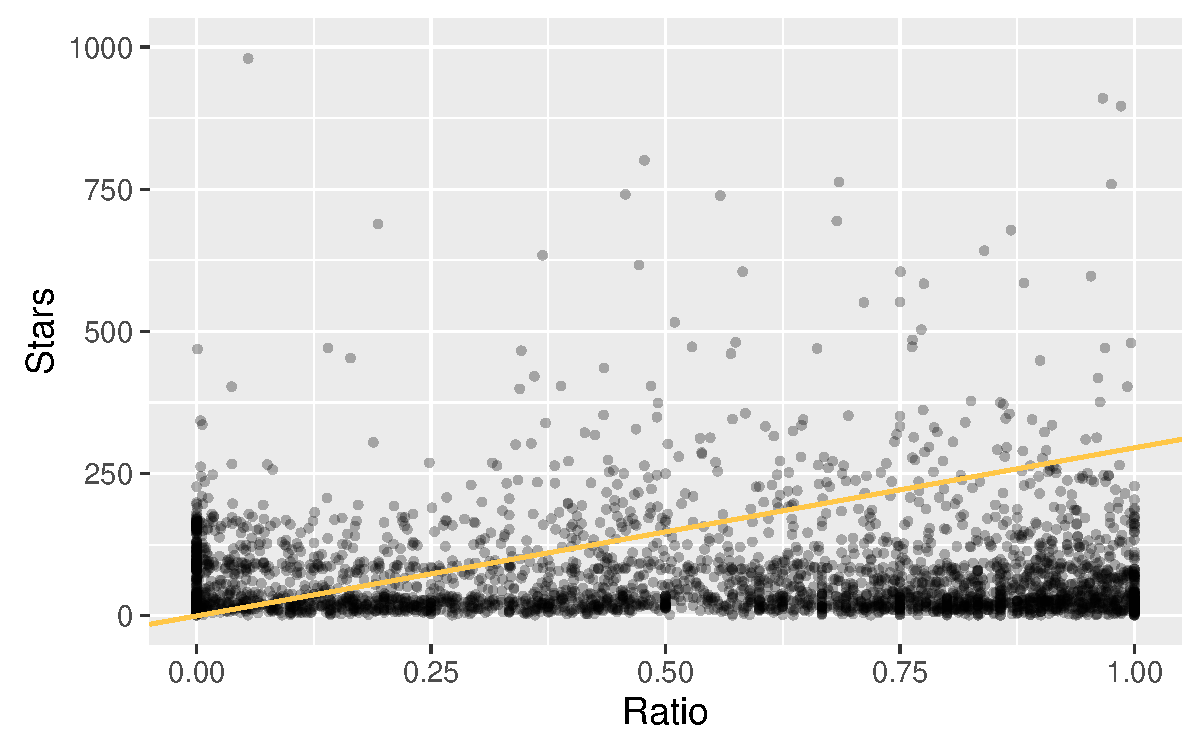
\includegraphics[page=1,scale=0.6]{../hypotheses/h3/ratio_subscriber_model_1.pdf}
	\captionof{figure}{Correlation coefficient (yellow slope) of "Ratio" on "Stars" (Model 3.1)}
	\label{fig:hyp3_m3.1}
\end{center}

\begin{landscape}
\subsubsection{H 3.1: Regression Tables}


\begin{table}[!h]
	\centering
	\scriptsize{
  	
% Table created by stargazer v.5.2 by Marek Hlavac, Harvard University. E-mail: hlavac at fas.harvard.edu
% Date and time: Sun, Mar 20, 2016 - 23:41:57
\begin{tabular}{@{\extracolsep{5pt}}lcccccccccccc}
\\[-1.8ex]\hline
\hline \\[-1.8ex]
 & \multicolumn{12}{c}{\textit{Dependent variable:}} \\
\cline{2-13}
\\[-1.8ex] & \multicolumn{4}{c}{Stars} & \multicolumn{4}{c}{Subscribers} & \multicolumn{4}{c}{Forks} \\
\\[-1.8ex] & (3.1) & (3.2) & (3.3) & (3.4) & (3.5) & (3.6) & (3.7) & (3.8) & (3.9) & (3.10) & (3.11) & (3.12)\\
\hline \\[-1.8ex]
 Ratio & 295.609$^{***}$ & 278.398$^{***}$ & 129.899 & 152.407$^{*}$ & 7.184 & 7.068 & 18.616$^{***}$ & 17.985$^{***}$ & 51.697$^{***}$ & 39.361$^{**}$ & 26.293 & 29.970 \\
  & (75.069) & (79.011) & (83.121) & (83.466) & (6.010) & (6.284) & (6.284) & (6.322) & (18.318) & (19.329) & (20.865) & (21.002) \\
  & & & & & & & & & & & & \\
 Age & 0.367$^{***}$ & 0.437$^{***}$ & 0.443$^{***}$ & 0.494$^{***}$ & 0.031$^{***}$ & 0.036$^{***}$ & 0.037$^{***}$ & 0.039$^{***}$ & 0.129$^{***}$ & 0.143$^{***}$ & 0.151$^{***}$ & 0.158$^{***}$ \\
  & (0.047) & (0.049) & (0.050) & (0.051) & (0.004) & (0.004) & (0.004) & (0.004) & (0.011) & (0.012) & (0.013) & (0.013) \\
  & & & & & & & & & & & & \\
 Constant & $-$0.236 & $-$70.590 & $-$434.208$^{***}$ & $-$764.217$^{***}$ & 48.363$^{***}$ & 47.700$^{***}$ & $-$20.544$^{*}$ & $-$39.926$^{***}$ & $-$23.486 & $-$43.139 & $-$113.655$^{***}$ & $-$192.851$^{***}$ \\
  & (60.212) & (154.968) & (139.704) & (195.611) & (4.821) & (12.325) & (10.562) & (14.817) & (14.692) & (37.910) & (35.069) & (49.222) \\
  & & & & & & & & & & & & \\
\hline \\[-1.8ex]
Observations & 3,419 & 3,419 & 3,419 & 3,419 & 3,419 & 3,419 & 3,419 & 3,419 & 3,419 & 3,419 & 3,419 & 3,419 \\
Log Likelihood & $-$29,905.750 & $-$29,877.320 & $-$29,692.650 & $-$29,668.010 & $-$21,273.000 & $-$21,221.860 & $-$20,863.760 & $-$20,845.730 & $-$25,083.110 & $-$25,063.340 & $-$24,966.870 & $-$24,950.480 \\
Akaike Inf. Crit. & 59,817.500 & 59,778.650 & 59,505.300 & 59,474.010 & 42,552.000 & 42,467.720 & 41,847.520 & 41,829.460 & 50,172.220 & 50,150.680 & 50,053.740 & 50,038.950 \\
\hline
\hline \\[-1.8ex]
\textit{Note:}  & \multicolumn{12}{r}{$^{*}$p$<$0.1; $^{**}$p$<$0.05; $^{***}$p$<$0.01} \\
\end{tabular}

	}
	\caption{Impact of "Age" and "Ratio" on "Stars", "Subscribers" and "Forks" through \textit{Fitting Generalized Linear Models} with dummy variables for \textit{Firms} and \textit{Programming Languages}. Using (a) dummy variables for each \textit{Firm} in model 3.3, 3.7 and 3.11 (b) dummy variables for each \textit{Language} in model 3.2, 3.6, 3.10 (c) dummy variables for each \textit{Firm and Language} in model 3.4, 3.8 and 3.12}
  \label{tbl:statistics_glm_project_popularity_short}
\end{table}

\begin{table}[!h]
	\centering
	\scriptsize{
  	
% Table created by stargazer v.5.2 by Marek Hlavac, Harvard University. E-mail: hlavac at fas.harvard.edu
% Date and time: Mon, Mar 21, 2016 - 00:04:00
\begin{tabular}{@{\extracolsep{5pt}}lcccccccccccc}
\\[-1.8ex]\hline
\hline \\[-1.8ex]
 & \multicolumn{12}{c}{\textit{Dependent variable:}} \\
\cline{2-13}
\\[-1.8ex] & \multicolumn{4}{c}{Number of Issues} & \multicolumn{4}{c}{Number of Contributors} & \multicolumn{4}{c}{Top Project} \\
\\[-1.8ex] & \multicolumn{4}{c}{\textit{normal}} & \multicolumn{4}{c}{\textit{normal}} & \multicolumn{4}{c}{\textit{logistic}} \\
\\[-1.8ex] & (3.13) & (3.14) & (3.15) & (3.16) & (3.17) & (3.18) & (3.19) & (3.20) & (3.21) & (3.22) & (3.23) & (3.24)\\
\hline \\[-1.8ex]
% \endhead
 Ratio & 2.147 & 2.006 & 7.861$^{*}$ & 7.612$^{*}$ & $-$2.417 & $-$2.647 & 1.391 & 1.402 & 2.025$^{***}$ & 1.727$^{***}$ & 1.906$^{***}$ & 1.753$^{***}$ \\
  & (3.717) & (3.930) & (4.235) & (4.275) & (1.911) & (2.005) & (2.051) & (2.067) & (0.155) & (0.166) & (0.191) & (0.197) \\
  & & & & & & & & & & & & \\
 Age & 0.015$^{***}$ & 0.017$^{***}$ & 0.021$^{***}$ & 0.022$^{***}$ & 0.018$^{***}$ & 0.019$^{***}$ & 0.020$^{***}$ & 0.021$^{***}$ & 0.001$^{***}$ & 0.001$^{***}$ & 0.001$^{***}$ & 0.001$^{***}$ \\
  & (0.002) & (0.002) & (0.003) & (0.003) & (0.001) & (0.001) & (0.001) & (0.001) & (0.0001) & (0.0001) & (0.0001) & (0.0001) \\
  & & & & & & & & & & & & \\
 Constant & 8.443$^{***}$ & $-$2.780 & $-$19.593$^{***}$ & $-$34.006$^{***}$ & 5.114$^{***}$ & 4.488 & $-$14.598$^{***}$ & $-$20.129$^{***}$ & $-$3.426$^{***}$ & $-$2.546$^{***}$ & $-$5.820$^{***}$ & $-$6.276$^{***}$ \\
  & (2.981) & (7.707) & (7.118) & (10.018) & (1.533) & (3.933) & (3.447) & (4.845) & (0.140) & (0.251) & (0.437) & (0.529) \\
  & & & & & & & & & & & & \\
\hline \\[-1.8ex]
Observations & 3,419 & 3,419 & 3,419 & 3,419 & 3,419 & 3,419 & 3,419 & 3,419 & 3,419 & 3,419 & 3,419 & 3,419 \\
Log Likelihood & $-$19,630.080 & $-$19,616.630 & $-$19,514.800 & $-$19,507.690 & $-$17,355.340 & $-$17,316.430 & $-$17,035.330 & $-$17,023.880 & $-$1,458.752 & $-$1,373.897 & $-$1,208.251 & $-$1,150.787 \\
Akaike Inf. Crit. & 39,266.160 & 39,257.260 & 39,149.610 & 39,153.370 & 34,716.680 & 34,656.870 & 34,190.660 & 34,185.760 & 2,923.504 & 2,771.795 & 2,536.502 & 2,439.574 \\
\hline
\hline \\[-1.8ex]
\textit{Note:}  & \multicolumn{12}{r}{$^{*}$p$<$0.1; $^{**}$p$<$0.05; $^{***}$p$<$0.01} \\
\end{tabular}

	}
	\caption{Impact of "Age" and "Ratio" on "Issues", "Contributors" and "Popularity" through \textit{Fitting Generalized Linear Models}. Using (a) dummy variables for each \textit{Firm} in model 3.15, 3.19 and 3.23 (b) dummy variables for each \textit{Language} in model 3.14, 3.18, 3.22 (c) dummy variables for each \textit{Firm and Language} in model 3.16, 3.20 and 3.24}
  \label{tbl:statistics_glm_project_popularity_short2}
\end{table}

\begin{table}
	\centering
	\footnotesize{
	  
% Table created by stargazer v.5.2 by Marek Hlavac, Harvard University. E-mail: hlavac at fas.harvard.edu
% Date and time: Mon, Mar 14, 2016 - 14:37:24
\begin{tabular}{@{\extracolsep{5pt}}lcccccc}
\\[-1.8ex]\hline
\hline \\[-1.8ex]
 & \multicolumn{6}{c}{\textit{Dependent variable:}} \\
\cline{2-7}
\\[-1.8ex] & Stars & Subscribers & Forks & Number of Issues & Number of Contributors & Top Project \\
\\[-1.8ex] & \textit{linear} & \textit{linear} & \textit{linear} & \textit{linear} & \textit{linear} & \textit{generalized linear} \\
 & \textit{mixed-effects} & \textit{mixed-effects} & \textit{mixed-effects} & \textit{mixed-effects} & \textit{mixed-effects} & \textit{mixed-effects} \\
\\[-1.8ex] & (3.25) & (3.26) & (3.27) & (3.28) & (3.29) & (3.30)\\
\hline \\[-1.8ex]
 Ratio & 149.245$^{*}$ & 18.379$^{***}$ & 31.783 & 5.896 & 1.235 & 1.910$^{***}$ \\
  & (82.032) & (6.237) & (20.266) & (4.111) & (2.032) & (0.185) \\
  & & & & & & \\
 Age & 0.420$^{***}$ & 0.036$^{***}$ & 0.142$^{***}$ & 0.020$^{***}$ & 0.020$^{***}$ & 0.001$^{***}$ \\
  & (0.049) & (0.004) & (0.012) & (0.002) & (0.001) & (0.0001) \\
  & & & & & & \\
 Constant & 160.468 & 44.443$^{***}$ & $-$9.606 & 2.911 & 2.225 & $-$3.497$^{***}$ \\
  & (104.513) & (9.753) & (21.187) & (4.280) & (2.974) & (0.235) \\
  & & & & & & \\
\hline \\[-1.8ex]
Observations & 3,419 & 3,419 & 3,419 & 3,419 & 3,419 & 3,419 \\
Log Likelihood & $-$29,774.830 & $-$20,966.900 & $-$25,031.110 & $-$19,582.970 & $-$17,137.260 & $-$1,298.686 \\
Akaike Inf. Crit. & 59,559.660 & 41,943.800 & 50,072.220 & 39,175.940 & 34,284.520 & 2,605.372 \\
Bayesian Inf. Crit. & 59,590.340 & 41,974.490 & 50,102.910 & 39,206.620 & 34,315.210 & 2,629.921 \\
\hline
\hline \\[-1.8ex]
\textit{Note:}  & \multicolumn{6}{r}{$^{*}$p$<$0.1; $^{**}$p$<$0.05; $^{***}$p$<$0.01} \\
\end{tabular}

	}
	\caption{Impact of "Age" and "Ratio" on projects' social metrics ("Stars", "Subscribers", "Forks" and "Issues") and popularity (is "Top Project" yes / no) through \textit{Mixed Model} between \textit{Firms}. "Number of Contributors" is just a control attribute and not a describing model.}
	\label{tbl:h3.1_mixed_models_popularity}
\end{table}

See regression table \ref{tbl:lmer_ratio_as_dependent_1} and \ref{tbl:lmer_ratio_as_dependent_2} (page \pageref{tbl:lmer_ratio_as_dependent_1} - \pageref{tbl:lmer_ratio_as_dependent_2}) for results having "Ratio" as dependent variable and table \ref{tbl:h3.1_mixed_models_size} (page \pageref{tbl:h3.1_mixed_models_size}) for \textit{Mixed Model} between Firms and Programming Languages.

\end{landscape}

\clearpage
\normalsize

\subsection{H 3: Results and Interpretation}

\textbf{The "Ratio" (i.e. the share of code commits by firm employed developers) has a significant positive impact on the popularity of a project.}

If we use "Stars" as a proxy for popularity, we can approve that the "Ratio" has a high positive influence on the likelihood that a project is (very) popular (correlation coefficient is 295, see model 3.1 in table \ref{tbl:statistics_glm_project_popularity_short}). This extends to "Subscribers" as well but with a lower impact (see model 3.7 and 3.8 in table \ref{tbl:statistics_glm_project_popularity_short}). "Forks" are also positively influenced by "Ratio" but also with a much lower correlation coefficient (see model 3.10 in table \ref{tbl:statistics_glm_project_popularity_short}). Interestingly enough, "Ratio" has no (significant) impact on the number of issues - but issue participation share has an impact on success and popularity (as shown in chapter \ref{sec:h1.2_h1.3_results_and_interpretation}).

Unfortunately, dummy variables (for \textit{Firms} and \textit{Programming Languages} respectively) have diverse effects on the regression results. This might be caused by different popularity attributes which are effected by different users' behavior. For example: \textit{JavaScript} developers could be more "Stargazer" friendly, \textit{C++} developer user more "Subscriber" friendly (and so on). Firms also may have different effects on specific popularity attributes: Some are more popular and some are less popular in the OS community (see the example of \textit{Microsoft} and \textit{GitHub} in chapter \ref{sec:atom_vs_vsc}).

Another broad hint is given by the \textit{logistic regression models}: \textbf{The probability that a project is a "Top Project" depends significant on the size of "Ratio"} (see model 3.21 - 3.24 in table \ref{tbl:statistics_glm_project_popularity_short2}). By using logistics regression we can interpret $\beta_{j}$ through $e^{\beta{j}}$ as effect coefficient \cite[p. 71]{agresti2007introduction}. Thus, the effect coefficient is between $e^{1.727} \approx 5.62$ and $e^{1.91} \approx 6.75$ \footnote{the problem of multicollinearity might reduce the validity of the mentioned effect coefficients, but seems to be rejected by results in observations over time (see chapter \ref{sec:h2_analysis})}.
 \textbf{This means that projects with highest "Ratios" are more likely "Top Projects" by the factor of 6.}


\newpage
%\addcontentsline{toc}{section}{Results}

\section{Results and Conclusion}
\label{sec:results}

All hypotheses are mainly confirmed by the empirical findings:

\begin{itemize}
  \item Through their code contribution firm employed developers have a strong positive impact on the code contribution of external developers
  \item Firm employed developers have a strong positive impact by participating on issues and comments in issues by causing more participation of external users
  \item The first year seems to be the most important time period for firm employed developers' participation: High contribution ratio in the beginning benefits popularity and success of the OS project in the long run
  \item The higher the overall share of contribution from firm employed developers, the more likely the project is successful and accepted by the OS community
\end{itemize}

Nevertheless, influence of higher participation of firm employed developers could not be verified ultimately on some continuous social metrics \footnote{\textit{Forks} and \textit{Number of Issues} on some models} which might be caused by broad difference of popularity and level of awareness between firms and software segments.

Beside the regression results we also receive interesting fringe insights: According to the frequency of commits with respect to daytime we can assume, that most firms and OS developers do work in USA, Canada and Europe. Also do external developers seem to be employed as well. Most developers commit source code at the usual working time period (9 a.m. - 5 p.m.) and "external developers" do not differ significantly from as "firm employed" classified developers. This would imply, that there is a stronger collaboration between firms than between firms and "libertine" developers.

\subsection{Implications and Managerial Advice}

Firms should initiate and invest \footnote{with funds and man-power} in their OS projects. The share of code contribution by firm employees should be very high - especially in the beginning - to achieve a broad acceptance by the OS community and developers on (rival) firms \footnote{contribution in the beginning can be interpreted as groundwork that needs to be done by firm employed developers to build a solid software foundation}. The return of investment will be a multiplier effect on commitment \footnote{via source code contribution and participation in communication channels} by external developers and a gain on level of awareness. Beside that, firms' OS commitment might lead to more cross-firm collaboration, improve employment of external developers and bring forward establishing new technologies in smaller amounts of time. If the share of firm employed developers is higher than usual, projects seem more likely to reach a certain degree of quality, maturity and attention. As result the community is willing to contribute their professional expertise for free to the project.

% As the selection of firms (by their number of popular projects) reveals, almost all well-known and favored software technology firms are represented.

\subsection{Further Research}
\label{sec:further_research}

The empirical data implies further research with respect to broader observations of firms and projects. By analyzing more firms and projects the hypotheses could eventually be applied more generally to software technology driven firms. Consideration of financial data of firms could reveal the impact of OS commitment on firms' revenue. And more sophisticated employees firm rating would help to investigate the coherence of OS commitment and quality of work environment. Furthermore, observations of network relations between firms, developers and users would improve the understanding of the importance of collaboration and exchange of knowledge.
%
% \begin{itemize}
%   \item observe all firms
%   \item firm financial data
%   \item firm / work place ratings by employees (developers)
%   \item collaboration between firm developers
%   \item measure firm reputation in open source communities (improves more OS commitment firm's reputation in the community / for potential employees)
% \end{itemize}

% \subsection{Outlook and Discussion}
%
% \begin{itemize}
%   \item further research (network effects, cross firm collaboration)
% \end{itemize}

% TODO: Results, Conclusion, Discussion


% Help tp Lontables
% Source: http://tex.stackexchange.com/questions/11380/how-to-repeat-top-rows-column-headings-on-every-page
% \documentclass{article}
% \usepackage{longtable}
% \begin{document}
% \begin{longtable}{ccc}
% \hline
% Column 1 & Column 2 & Column 3\\
% \hline
% \endhead % all the lines above this will be repeated on every page
% A & B & C\\
% A & B & C\\
% ... many lines of table ...
% \end{longtable}
% \end{document}
% --> \endhead




% ----------------
% --- appendix ---
% ----------------
\appendix

\newpage
\pagestyle{plain}
%\addcontentsline{toc}{section}{Listings}
\section{Listings}

\footnotesize
\lstinputlisting[
  language=SQL,
  caption={BigQuery via GitHubArchive},
  label={lst:githubusersandprojectscount}
]{../listings/githubusersandprojectscount.sql}

\lstinputlisting[
  label={lst:gitcommit},
  caption={Structure of a git commit}
]{../listings/git_commit.sh}

\lstinputlisting[
  language=R,
  label={lst:lm_h1.1},
  caption={Linear regression models in R for H 1.1}
]{../listings/lm_h1.1.R}

\lstinputlisting[
  language=R,
  label={lst:lm_h1.2},
  caption={Linear regression models in R for H 1.2}
]{../listings/lm_h1.2.R}

\lstinputlisting[
  language=R,
  label={lst:lm_h1.3},
  caption={Linear regression models in R for H 1.3}
]{../listings/lm_h1.3.R}

\lstinputlisting[
  language=R,
  label={lst:lm_h2.1},
  caption={Linear regression models in R for H 2.1}
]{../listings/lm_h2.1.R}

\lstinputlisting[
  language=R,
  label={lst:lm_h3.1},
  caption={Linear regression models in R for H 3.1}
]{../listings/lm_h3.1.R}

\normalsize



% tables (not mandatory)
\newpage
\pagestyle{plain}
%\addcontentsline{toc}{section}{Tables}
%\setcounter{table}{0}
%\renewcommand{\thetable}{A\arabic{table}}
\normalsize
\section{Tables}

\subsection{Introduction and Theory}

\begin{table}[ht]
\centering
\begin{tabular}{rllll}
  \hline
 & Linux & FreeBSD & Unknown & MS.Windows \\
  \hline
W3Techs (02-2015) & 35.9\% & 0.95\% & 30.9\% & 32.3\% \\
  W3cook (05-2015) & 96.6\% & 1.7\% & 0\% & 1.7\% \\
   \hline
\end{tabular}
\caption{Share of Operating Systems on public Internet Servers; \textit{Sources: \url{http://w3techs.com/technologies/overview/operating_system/all}, \url{http://w3techs.com/technologies/details/os-unix/all/all}, \url{http://www.w3cook.com/os/summary/}}}
\label{tbl:publicserver2015}
\end{table}

\begin{table}[!h]
\centering
% Table created by stargazer v.5.2 by Marek Hlavac, Harvard University. E-mail: hlavac at fas.harvard.edu
% Date and time: Sat, Mar 26, 2016 - 18:58:30
% \begin{table}[!htbp] \centering
%   \caption{}
%   \label{}
\begin{tabular}{@{\extracolsep{5pt}}lccccc}
\\[-1.8ex]\hline
\hline \\[-1.8ex]
Statistic & \multicolumn{1}{c}{N} & \multicolumn{1}{c}{Mean} & \multicolumn{1}{c}{St. Dev.} & \multicolumn{1}{c}{Min} & \multicolumn{1}{c}{Max} \\
\hline \\[-1.8ex]
Top Project (yes/no) & 177 & 0.181 & 0.386 & 0 & 1 \\
Ratio & 177 & 0.684 & 0.334 & 0.000 & 1.000 \\
Age (days) & 177 & 294.260 & 226.632 & 20 & 1,466 \\
Number of Commits & 177 & 1,241.955 & 10,558.430 & 3 & 127,063 \\
Firm Employees' Commits & 177 & 138.073 & 307.597 & 0 & 2,573 \\
External Developers' Commits & 177 & 1,103.881 & 10,548.850 & 0 & 126,912 \\
Stars & 177 & 186.051 & 580.191 & 0 & 4,909 \\
Contributors & 177 & 9.949 & 27.287 & 2 & 262 \\
Subscribers & 177 & 50.655 & 71.049 & 2 & 585 \\
Forks & 177 & 45.153 & 155.701 & 0 & 1,812 \\
Number of Issues & 177 & 15.429 & 43.100 & 1 & 420 \\
\hline \\[-1.8ex]
\end{tabular}
% \end{table} 

\caption{Statistic of Projects by Microsoft}
\label{tbl:summary_microsoft}
\end{table}

\begin{table}[!h]
\centering
% Table created by stargazer v.5.2 by Marek Hlavac, Harvard University. E-mail: hlavac at fas.harvard.edu
% Date and time: Sat, Mar 26, 2016 - 18:58:04
% \begin{table}[!htbp] \centering
%   \caption{}
%   \label{}
\begin{tabular}{@{\extracolsep{5pt}}lccccc}
\\[-1.8ex]\hline
\hline \\[-1.8ex]
Statistic & \multicolumn{1}{c}{N} & \multicolumn{1}{c}{Mean} & \multicolumn{1}{c}{St. Dev.} & \multicolumn{1}{c}{Min} & \multicolumn{1}{c}{Max} \\
\hline \\[-1.8ex]
Top Project (yes/no) & 40 & 0.400 & 0.496 & 0 & 1 \\
Ratio & 40 & 0.528 & 0.333 & 0.000 & 1.000 \\
Age (days) & 40 & 1,039.925 & 615.875 & 62 & 2,449 \\
Number of Commits & 40 & 1,784.450 & 7,037.635 & 5 & 44,486 \\
Firm Employees' Commits & 40 & 290.175 & 516.544 & 0 & 1,905 \\
External Developers' Commits & 40 & 1,494.275 & 7,021.648 & 0 & 44,482 \\
Stars & 40 & 993.175 & 1,705.672 & 1 & 7,922 \\
Contributors & 40 & 56.625 & 114.295 & 2 & 451 \\
Subscribers & 40 & 62.750 & 62.040 & 6 & 233 \\
Forks & 40 & 244.350 & 518.172 & 1 & 2,611 \\
Number of Issues & 40 & 20.500 & 43.776 & 1 & 242 \\
\hline \\[-1.8ex]
\end{tabular}
% \end{table}

\caption{Statistic of Projects by GitHub}
\label{tbl:summary_github}
\end{table}

\begin{table}[!h]
\centering
% Table created by stargazer v.5.2 by Marek Hlavac, Harvard University. E-mail: hlavac at fas.harvard.edu
% Date and time: Sat, Mar 26, 2016 - 18:57:38
% \begin{table}[!htbp] \centering
%   \caption{}
%   \label{}
\begin{tabular}{@{\extracolsep{5pt}}lccccc}
\\[-1.8ex]\hline
\hline \\[-1.8ex]
Statistic & \multicolumn{1}{c}{N} & \multicolumn{1}{c}{Mean} & \multicolumn{1}{c}{St. Dev.} & \multicolumn{1}{c}{Min} & \multicolumn{1}{c}{Max} \\
\hline \\[-1.8ex]
Top Project (yes/no) & 103 & 0.534 & 0.501 & 0 & 1 \\
Ratio & 103 & 0.591 & 0.342 & 0.000 & 1.000 \\
Age (days) & 103 & 731.204 & 517.623 & 79 & 2,489 \\
Number of Commits & 103 & 1,103.039 & 4,112.523 & 5 & 36,596 \\ 
Firm Employees' Commits & 103 & 559.748 & 1,682.788 & 0 & 14,499 \\
External Developers' Commits & 103 & 543.291 & 3,553.457 & 0 & 35,872 \\
Stars & 103 & 2,360.272 & 4,762.077 & 12 & 35,214 \\
Contributors & 103 & 36.767 & 70.711 & 2 & 468 \\
Subscribers & 103 & 188.990 & 347.568 & 16 & 2,617 \\
Forks & 103 & 396.107 & 854.878 & 2 & 5,716 \\
Number of Issues & 103 & 56.029 & 161.550 & 1 & 1,043 \\
\hline \\[-1.8ex]
\end{tabular}
% \end{table}

\caption{Statistic of Projects by facebook}
\label{tbl:summary_facebook}
\end{table}

\clearpage
\subsection{Data and Basic Statistics Tables}

	% latex table generated in R 3.2.2 by xtable 1.8-0 package
% Tue Feb  9 23:24:08 2016
{\footnotesize
\begin{longtable}{rlrl}

  \hline
 & Name of Organization on GitHub & Top Repositories & is commercial Organization \\
  \hline
  \endhead
  1 & google &  85 & yes \\
    2 & facebook &  56 & yes \\
    3 & Microsoft &  33 & yes \\
    4 & square &  30 & yes \\
    5 & apache &  23 & partly \\
    6 & aspnet &  23 & partly \\
    7 & thoughtbot &  23 & yes \\
    8 & alibaba &  19 & yes \\
    9 & mozilla &  18 & partly \\
    10 & twitter &  18 & yes \\
    11 & Netflix &  17 & yes \\
    12 & github &  16 & yes \\
    13 & mongodb &  16 & yes \\
    14 & mono &  16 & no \\
    15 & thephpleague &  16 & no \\
    16 & docker &  15 & yes \\
    17 & elastic &  15 & yes \\
    18 & hashicorp &  15 & yes \\
    19 & golang &  14 & partly \\
    20 & Yalantis &  13 & yes \\
    21 & dotnet &  12 & partly \\
    22 & rails &  12 & partly \\
    23 & airbnb &  10 & yes \\
    24 & aws &  10 & yes \\
    25 & etsy &  10 & yes \\
    26 & googlesamples &  10 & yes \\
    27 & linkedin &  10 & yes \\
    28 & xamarin &  10 & yes \\
    29 & zeromq &  10 & no \\
    30 & coreos &   9 & partly \\
    31 & laravel &   9 & no \\
    32 & Shopify &   9 & yes \\
    33 & spring-projects &   9 & partly \\
    34 & adafruit &   8 & yes \\
    35 & bitly &   8 & yes \\
    36 & dmlc &   8 & no \\
    37 & doctrine &   8 & no \\
    38 & facebookarchive &   8 & partly \\
    39 & fastlane &   8 & no \\
    40 & jquery &   8 & no \\
    41 & KnpLabs &   8 & yes \\
    42 & shadowsocks &   8 & no \\
    43 & Yelp &   8 & yes \\
    44 & apple &   7 & yes \\
    45 & Automattic &   7 & yes \\
    46 & Azure &   7 & yes \\
    47 & cocos2d &   7 & no \\
    48 & couchbase &   7 & no \\
    49 & douban &   7 & yes \\
    50 & FriendsOfPHP &   7 & no \\
    51 & id-Software &   7 & yes \\
    52 & libgit2 &   7 & no \\
    53 & stripe &   7 & yes \\
    54 & cloudera &   6 & yes \\
    55 & dropbox &   6 & yes \\
    56 & enormego &   6 & yes \\
    57 & Homebrew &   6 & no \\
    58 & icsharpcode &   6 & no \\
    59 & msgpack &   6 & no \\
    60 & nodejs &   6 & no \\
    61 & openresty &   6 & no \\
    62 & ParsePlatform &   6 & yes \\
    63 & raspberrypi &   6 & partly \\
    64 & spotify &   6 & yes \\
    65 & twilio &   6 & yes \\
    66 & yahoo &   6 & yes \\
    67 & android &   5 & partly \\
    68 & angular &   5 & partly \\
    69 & angular-ui &   5 & partly \\
    70 & applidium &   5 & yes \\
    71 & celluloid &   5 & no \\
    72 & cesanta &   5 & yes \\
    73 & cucumber &   5 & yes \\
    74 & FriendsOfSymfony &   5 & no \\
    75 & heroku &   5 & yes \\
    76 & JetBrains &   5 & partly \\
    77 & paypal &   5 & yes \\
    78 & plataformatec &   5 & yes \\
    79 & RailsApps &   5 & no \\
    80 & rspec &   5 & no \\
    81 & ServiceStack &   5 & yes \\
    82 & socketio &   5 & no \\
    83 & ValveSoftware &   5 & yes \\
    84 & VerbalExpressions &   5 & no \\
    85 & visionmedia &   5 & no \\
    86 & activerecord-hackery &   4 & no \\
    87 & CakeDC &   4 & partly \\
    88 & castleproject &   4 & no \\
    89 & chef &   4 & yes \\
    90 & collectiveidea &   4 & yes \\
    91 & composer &   4 & no \\
    92 & docopt &   4 & no \\
    93 & documentcloud &   4 & partly \\
    94 & Flipboard &   4 & yes \\
    95 & forkingdog &   4 & no \\
    96 & getsentry &   4 & yes \\
    97 & gliderlabs &   4 & yes \\
    98 & gorilla &   4 & no \\
    99 & Instagram &   4 & yes \\
    100 & intridea &   4 & yes \\
    101 & mapbox &   4 & yes \\
    102 & mutualmobile &   4 & yes \\
    103 & openstack &   4 & yes \\
    104 & owncloud &   4 & yes \\
    105 & phacility &   4 & yes \\
    106 & Qihoo360 &   4 & yes \\
    107 & Reactive-Extensions &   4 & yes \\
    108 & sass &   4 & no \\
    109 & sourcegraph &   4 & yes \\
    110 & symfony &   4 & partly \\
    111 & tumblr &   4 & yes \\
    112 & venmo &   4 & yes \\
    113 & yhat &   4 & yes \\
   \hline
   \caption{All Organizations having at least 4 top repositories}
   \label{tbl:organizations_with_top_repos}

\end{longtable}


	\begin{landscape}
		\footnotesize{
			% latex table generated in R 3.2.2 by xtable 1.7-4 package
% Sun Oct 11 16:20:54 2015

\begin{longtable}{rlrrrrrrrrrrrrrr}
  % \centering
  % \footnotesize
  % \begin{tabular}
    \hline
   & Firm & Repos & JS & ObjC & Go & C & Python & Ruby & Java & PHP & C++ & C\# & CS & Scala & Hack \\
    \hline
  1 & google &  79 &   6 &  &  15 &   6 &   8 &   1 &  16 &   3 &  23 &   1 &  &  &  \\
    2 & facebook &  58 &  10 &   9 &  &   7 &   4 &  &  10 &   2 &  14 &  &  &  &   2 \\
    3 & twitter &  48 &   3 &   2 &  &   4 &  &   3 &   4 &  &   2 &  &  &  30 &  \\
    4 & Microsoft &  21 &   1 &  &  &   2 &  &  &  &  &   8 &  10 &  &  &  \\
    5 & github &  20 &   1 &   1 &   3 &   1 &  &   8 &  &  &  &   2 &   4 &  &  \\
    6 & alibaba &  20 &  &  &  &   4 &  &  &  12 &  &   4 &  &  &  &  \\
    7 & linkedin &  12 &   2 &   2 &  &  &  &  &   7 &  &  &  &   1 &  &  \\
    8 & aws \tablefootnote{by Amazon.com} &  11 &   1 &   1 &   2 &  &   1 &   2 &   1 &   2 &  &   1 &  &  &  \\
    9 & yahoo &   6 &   2 &  &   1 &   1 &  &  &   1 &  &  &  &  &   1 &  \\
    10 & groupon &   4 &  &  &  &  &  &  &  &  &  &  &   4 &  &  \\
    11 & NetEase &   2 &   1 &  &  &  &  &  &  &  &  &   1 &  &  &  \\
    12 & yandex &   2 &  &  &  &  &   1 &  &  &  &   1 &  &  &  &  \\
    13 & eBay &   2 &  &  &  &  &   2 &  &  &  &  &  &  &  &  \\
    14 & SonyWWS &   2 &  &  &  &  &  &  &  &  &  &   2 &  &  &  \\
    15 & sony &   1 &  &  &   1 &  &  &  &  &  &  &  &  &  &  \\
    16 & awslabs \tablefootnote{by Amazon.com} &   1 &  &  &  &   1 &  &  &  &  &  &  &  &  &  \\
    17 & intel-iot-devkit &   1 &  &  &  &   1 &  &  &  &  &  &  &  &  &  \\
    18 & forcedotcom \tablefootnote{by Salesforce} &   1 &  &  &  &  &  &  &   1 &  &  &  &  &  &  \\
    19 & amazonwebservices \tablefootnote{by Amazon.com} &   1 &  &  &  &  &  &  &  &   1 &  &  &  &  &  \\
    20 & developerforce \tablefootnote{by Salesforce} &   1 &  &  &  &  &  &  &  &  &  &   1 &  &  &  \\
     \hline
  % \end{tabular}
  \caption{Commercial most succesfull and most popular companies and their \textit{GitHub} projects' programming languages. \textit{Source: GitHub API, October 2015} }
  \label{tbl:commercial_successfull_firms_on_github_with_languages}
\end{longtable}

		}
	\end{landscape}

	{\footnotesize
		% latex table generated in R 3.2.2 by xtable 1.8-0 package
% Wed Feb 10 09:27:17 2016

\begin{longtable}{rlllrlr}


  \hline
 & Name & Name on GitHub & Public Repositories & Top Repositories & On GitHub since \\
  \hline
  \endhead
1 & Adafruit Industries & adafruit & 469 &   8 & 2010 \\
  2 & Airbnb & airbnb &  86 &  10 & 2011 \\
  3 & Alibaba & alibaba &  87 &  19 & 2012 \\
  4 & Apple & apple &  18 &   7 & 2015 \\
  5 & Applidium & applidium &  15 &   5 & 2010 \\
  6 & Automattic & Automattic & 279 &   7 & 2011 \\
  7 & Amazon Web Services & aws &  49 &  10 & 2012 \\
  8 & Microsoft Azure & Azure & 148 &   7 & 2014 \\
  9 & Bitly & bitly &  26 &   8 & 2010 \\
  10 & Cesanta Software & cesanta &  24 &   5 & 2013 \\
  11 & Chef Software, Inc. & chef & 284 &   4 & 2008 \\
  12 & Cloudera & cloudera & 133 &   6 & 2009 \\
  13 & Collective Idea & collectiveidea & 155 &   4 & 2008 \\
  14 & (Cucumber) & (cucumber) &  (52) &   (5) & 2010 \\
  15 & Docker & docker &  64 &  15 & 2013 \\
  16 & Douban Inc. & douban &  38 &   7 & 2011 \\
  17 & Dropbox & dropbox & 104 &   6 & 2011 \\
  18 & elastic & elastic & 107 &  15 & 2014 \\
  19 & (enormego) & (enormego) &  (26) &   (6) & 2009 \\
  20 & Etsy, Inc. & etsy &  56 &  10 & 2010 \\
  21 & Facebook & facebook & 149 &  56 & 2009 \\
  22 & Flipboard & Flipboard &  19 &   4 & 2010 \\
  23 & (Sentry) & (getsentry) &  (79) &   (4) & 2012 \\
  24 & GitHub & github & 127 &  16 & 2008 \\
  25 & (Glider Labs) & (gliderlabs) &  (19) &   (4) & 2014 \\
  26 & Google & google & 681 &  85 & 2012 \\
  27 & Google Samples & googlesamples & 184 &  10 & 2014 \\
  28 & HashiCorp & hashicorp &  79 &  15 & 2011 \\
  29 & Heroku & heroku & 488 &   5 & 2008 \\
  30 & id Software & id-Software &  18 &   7 & 2012 \\
  31 & Instagram & Instagram &  25 &   4 & 2011 \\
  32 & INTRIDEA Inc. & intridea & 107 &   4 & 2008 \\
  33 & KNP Labs & KnpLabs &  92 &   8 & 2010 \\
  34 & LinkedIn & linkedin &  87 &  10 & 2010 \\
  35 & Mapbox & mapbox & 558 &   4 & 2011 \\
  36 & Microsoft & Microsoft & 405 &  33 & 2013 \\
  37 & mongodb & mongodb &  54 &  16 & 2009 \\
  38 & Mutual Mobile & mutualmobile &  60 &   4 & 2009 \\
  39 & Netflix, Inc. & Netflix &  99 &  17 & 2011 \\
  40 & OpenStack & openstack & 665 &   4 & 2010 \\
  41 & ownCloud & owncloud &  95 &   4 & 2012 \\
  42 & Parse & ParsePlatform &  56 &   6 & 2011 \\
  43 & PayPal & paypal & 140 &   5 & 2010 \\
  44 & Phacility & phacility &   6 &   4 & 2013 \\
  45 & (Plataformatec) & (plataformatec) &  (23) &   (5) & 2009 \\
  46 & Qihoo 360 & Qihoo360 &  17 &   4 & 2013 \\
  47 & Cloud Programmability Group & Reactive-Extensions &  38 &   4 & 2011 \\
  48 & (ServiceStack) & (ServiceStack) &  (32) &   (5) & 2011 \\
  49 & Shopify & Shopify & 265 &   9 & 2008 \\
  50 & Sourcegraph & sourcegraph & 150 &   4 & 2013 \\
  51 & Spotify & spotify & 131 &   6 & 2010 \\
  52 & Square & square & 157 &  30 & 2009 \\
  53 & Stripe & stripe &  66 &   7 & 2011 \\
  54 & thoughtbot, inc. & thoughtbot & 221 &  23 & 2008 \\
  55 & Tumblr & tumblr &  34 &   4 & 2010 \\
  56 & Twilio & twilio &  47 &   6 & 2009 \\
  57 & Twitter, Inc. & twitter & 135 &  18 & 2009 \\
  58 & Valve Software & ValveSoftware &  17 &   5 & 2012 \\
  59 & Venmo & venmo &  73 &   4 & 2010 \\
  60 & Xamarin & xamarin &  78 &  10 & 2011 \\
  61 & Yahoo Inc. & yahoo & 330 &   6 & 2008 \\
  62 & Yalantis & Yalantis &  36 &  13 & 2011 \\
  63 & Yelp.com & Yelp & 149 &   8 & 2009 \\
  64 & yhat & yhat & 102 &   4 & 2012 \\
   \hline

   \caption{Finally selected commercial firms for observation. Bracketed firms are sorted out since they are not using an united webdomain. \\ \\
   \textbf{Data source:} \\
   \tiny
   \url{https://git.zeitpulse.com/philipp/masterthesis-data/raw/master/csv/organizations.csv} \\
   \url{https://git.zeitpulse.com/philipp/masterthesis-data/raw/master/csv/commercial_classification/commercial_classification_of_organizations.csv}
   }
   \label{tbl:selected_commercial_firms}

 \end{longtable}

	}

	\begin{landscape}
	\begin{table}[!h] \centering
		{\footnotesize
		% latex table generated in R 3.2.2 by xtable 1.8-0 package
% Wed Feb 10 19:54:22 2016


\begin{tabular}{rlrrlrrrrr}



  \hline
 & Firm & Rating & Ratings count & Level & Culture and Values & Career Opportunities & Work-Life-Balance & OS Repos. & Top Repos. count \\
  \hline
1 & elastic & 4.90 &  62 & Very Satisfied & 4.80 & 4.80 & 4.50 & 107 &  15 \\
  2 & Facebook & 4.50 & 1297 & Very Satisfied & 4.50 & 4.30 & 3.70 & 149 &  56 \\
  3 & Airbnb & 4.50 & 299 & Very Satisfied & 4.70 & 4.30 & 3.90 &  86 &  10 \\
  4 & Google & 4.40 & 4665 & Very Satisfied & 4.40 & 4.00 & 4.00 & 681 &  85 \\
  5 & Square & 4.40 & 155 & Very Satisfied & 4.30 & 4.00 & 4.10 & 157 &  30 \\
  6 & Google Samples & 4.40 & 4665 & Very Satisfied & 4.40 & 4.00 & 4.00 & 184 &  10 \\
  7 & LinkedIn & 4.40 & 1340 & Very Satisfied & 4.50 & 4.10 & 4.10 &  87 &  10 \\
  8 & Etsy, Inc. & 4.30 &  38 & Very Satisfied & 4.30 & 3.50 & 4.20 &  56 &  10 \\
  9 & Twitter, Inc. & 4.00 & 400 & Satisfied & 4.10 & 3.70 & 4.00 & 135 &  18 \\
  10 & mongodb & 4.00 & 135 & Satisfied & 4.00 & 4.00 & 3.80 &  54 &  16 \\
  11 & Microsoft & 3.90 & 12492 & Satisfied & 3.70 & 3.60 & 3.60 & 405 &  33 \\
  12 & Alibaba & 3.90 &  42 & Satisfied & 3.90 & 4.00 & 3.40 &  87 &  19 \\
  13 & Netflix, Inc. & 3.70 & 544 & Satisfied & 3.90 & 3.40 & 3.40 &  99 &  17 \\
  14 & Amazon Web Services & 3.40 & 7572 & OK & 3.30 & 3.40 & 2.70 &  49 &  10 \\
   \hline

\end{tabular}

		}
		\caption{Firm ratings by employees (\textit{Source: Glassdoor API, 25.01.2016})}
		\label{tbl:glassdoor_firm_ratings}
	\end{table}
	\end{landscape}

\clearpage
\subsection{Regression Tables for H 1.1}
\label{sec:regression_tables_h1.1}

	\begin{table}[!h] \centering
	  \scriptsize{
		  
% Table created by stargazer v.5.2 by Marek Hlavac, Harvard University. E-mail: hlavac at fas.harvard.edu
% Date and time: Tue, Mar 15, 2016 - 11:34:23
\begin{tabular}{@{\extracolsep{5pt}}lcccc}
\\[-1.8ex]\hline
\hline \\[-1.8ex]
 & \multicolumn{4}{c}{\textit{Dependent variable:}} \\
\cline{2-5}
\\[-1.8ex] & ext. commits & int. commits & ext. commits & int. commits \\
\\[-1.8ex] & (1.1.5) & (1.1.6) & (1.1.7) & (1.1.8)\\ 
\hline \\[-1.8ex]
 int. commits & 5.566$^{***}$ &  & 0.453$^{***}$ &  \\
  & (0.448) &  & (0.075) &  \\
  & & & & \\
 ext. commits &  & 0.009$^{***}$ &  & 0.156$^{***}$ \\
  &  & (0.001) &  & (0.026) \\
  & & & & \\
 Constant & $-$145.306 & 100.309$^{***}$ & 381.728$^{**}$ & 710.625$^{***}$ \\
  & (166.753) & (6.572) & (167.964) & (93.460) \\
  & & & & \\
\hline \\[-1.8ex]
Observations & 2,809 & 2,809 & 478 & 478 \\
R$^{2}$ & 0.052 & 0.052 & 0.071 & 0.071 \\
Adjusted R$^{2}$ & 0.052 & 0.052 & 0.069 & 0.069 \\
Residual Std. Error & 8,483.016 (df = 2807) & 347.859 (df = 2807) & 3,408.818 (df = 476) & 1,997.843 (df = 476) \\
F Statistic & 154.275$^{***}$ (df = 1; 2807) & 154.275$^{***}$ (df = 1; 2807) & 36.143$^{***}$ (df = 1; 476) & 36.143$^{***}$ (df = 1; 476) \\
\hline
\hline \\[-1.8ex]
\textit{Note:}  & \multicolumn{4}{r}{$^{*}$p$<$0.1; $^{**}$p$<$0.05; $^{***}$p$<$0.01} \\
\end{tabular}

	  }
		\caption{Impact of internal commits on external commits (and v.v.) on "Residual Projects" (Model 1.1.5 - 1.1.6) and "Top Projects" older than 1 year (Model 1.1.7 - 1.1.8)}
		\label{tbl:regression_table_1.1.5-1.1.7}
	\end{table}

	\begin{table}[!h] \centering
	  \scriptsize{
		  
% Table created by stargazer v.5.2 by Marek Hlavac, Harvard University. E-mail: hlavac at fas.harvard.edu
% Date and time: Tue, Mar 15, 2016 - 11:34:25
\begin{tabular}{@{\extracolsep{5pt}}lcccc}
\\[-1.8ex]\hline
\hline \\[-1.8ex]
 & \multicolumn{4}{c}{\textit{Dependent variable:}} \\
\cline{2-5}
\\[-1.8ex] & ext. commits & int. commits & ext. commits & int. commits \\
\\[-1.8ex] & (1.1.9) & (1.1.10) & (1.1.11) & (1.1.12)\\ 
\hline \\[-1.8ex]
 int. commits & 5.751$^{***}$ &  & 0.936$^{***}$ &  \\
  & (0.528) &  & (0.040) &  \\
  & & & & \\
 ext. commits &  & 0.010$^{***}$ &  & 0.864$^{***}$ \\
  &  & (0.001) &  & (0.037) \\
  & & & & \\
 Constant & $-$238.115 & 121.186$^{***}$ & $-$318.675 & 519.123$^{**}$ \\
  & (232.686) & (9.417) & (249.478) & (236.770) \\
  & & & & \\
\hline \\[-1.8ex]
Observations & 1,900 & 1,900 & 132 & 132 \\
R$^{2}$ & 0.059 & 0.059 & 0.809 & 0.809 \\
Adjusted R$^{2}$ & 0.058 & 0.058 & 0.807 & 0.807 \\
Residual Std. Error & 9,718.195 (df = 1898) & 409.982 (df = 1898) & 2,805.891 (df = 130) & 2,694.891 (df = 130) \\
F Statistic & 118.705$^{***}$ (df = 1; 1898) & 118.705$^{***}$ (df = 1; 1898) & 550.484$^{***}$ (df = 1; 130) & 550.484$^{***}$ (df = 1; 130) \\
\hline
\hline \\[-1.8ex]
\textit{Note:}  & \multicolumn{4}{r}{$^{*}$p$<$0.1; $^{**}$p$<$0.05; $^{***}$p$<$0.01} \\
\end{tabular}

	  }
		\caption{Impact of internal commits on external commits (and v.v.) on "Residual Projects" older than 1 year (Model 1.1.9 - 1.1.10) and "Top Projects" younger than 1 year (Model 1.1.11 - 1.1.12)}
		\label{tbl:regression_table_1.1.9-1.1.12}
	\end{table}

	\begin{table}[!h] \centering
	  \scriptsize{
		  
% Table created by stargazer v.5.2 by Marek Hlavac, Harvard University. E-mail: hlavac at fas.harvard.edu
% Date and time: Tue, Mar 15, 2016 - 11:34:26
\begin{tabular}{@{\extracolsep{5pt}}lcc}
\\[-1.8ex]\hline
\hline \\[-1.8ex]
 & \multicolumn{2}{c}{\textit{Dependent variable:}} \\
\cline{2-3}
\\[-1.8ex] & ext. commits & int. commits \\
\\[-1.8ex] & (1.1.13) & (1.1.14)\\ 
\hline \\[-1.8ex]
 int. commits & 2.323$^{*}$ &  \\
  & (1.225) &  \\
  & & \\
 ext. commits &  & 0.002$^{*}$ \\
  &  & (0.001) \\
  & & \\
 Constant & 190.823 & 58.289$^{***}$ \\
  & (180.326) & (4.483) \\
  & & \\
\hline \\[-1.8ex]
Observations & 909 & 909 \\
R$^{2}$ & 0.004 & 0.004 \\
Adjusted R$^{2}$ & 0.003 & 0.003 \\
Residual Std. Error (df = 907) & 4,983.821 & 134.877 \\
F Statistic (df = 1; 907) & 3.598$^{*}$ & 3.598$^{*}$ \\
\hline
\hline \\[-1.8ex]
\textit{Note:}  & \multicolumn{2}{r}{$^{*}$p$<$0.1; $^{**}$p$<$0.05; $^{***}$p$<$0.01} \\
\end{tabular}

	  }
		\caption{Impact of internal commits on external commits (and v.v.) on "Residual Projects" younger than 1 year (Model 1.1.13 - 1.1.14)}
		\label{tbl:regression_table_1.1.13-1.1.14}
	\end{table}


\clearpage
\subsection{Regression Tables for H 1.2.1}
\label{sec:regression_tables_h1.2.1}

	\begin{table}[!h] \centering
	  \scriptsize{
		  
% Table created by stargazer v.5.2 by Marek Hlavac, Harvard University. E-mail: hlavac at fas.harvard.edu
% Date and time: Tue, Mar 15, 2016 - 20:38:57
\begin{tabular}{@{\extracolsep{5pt}}lcccc}
\\[-1.8ex]\hline
\hline \\[-1.8ex]
 & \multicolumn{4}{c}{\textit{Dependent variable:}} \\
\cline{2-5}
\\[-1.8ex] & issues by ext. users & issues by firm empl. users & issues by ext. users & issues by firm empl. users \\
\\[-1.8ex] & (5) & (6) & (7) & (8)\\
\hline \\[-1.8ex]
 issues by firm empl. users & 5.211$^{***}$ &  & 34.605$^{***}$ &  \\
  & (0.448) &  & (2.815) &  \\
  & & & & \\
 issues by ext. users &  & 0.010$^{***}$ &  & 0.008$^{***}$ \\
  &  & (0.001) &  & (0.001) \\
  & & & & \\
 Constant & 40.005$^{***}$ & 0.357$^{***}$ & 242.496$^{***}$ & 2.892$^{***}$ \\
  & (2.717) & (0.125) & (47.815) & (0.724) \\
  & & & & \\
\hline \\[-1.8ex]
Observations & 2,412 & 2,412 & 414 & 414 \\
R$^{2}$ & 0.053 & 0.053 & 0.268 & 0.268 \\
Adjusted R$^{2}$ & 0.053 & 0.053 & 0.267 & 0.267 \\
Residual Std. Error & 132.237 (df = 2410) & 5.851 (df = 2410) & 898.292 (df = 412) & 13.449 (df = 412) \\
F Statistic & 135.324$^{***}$ (df = 1; 2410) & 135.324$^{***}$ (df = 1; 2410) & 151.164$^{***}$ (df = 1; 412) & 151.164$^{***}$ (df = 1; 412) \\
\hline
\hline \\[-1.8ex]
\textit{Note:}  & \multicolumn{4}{r}{$^{*}$p$<$0.1; $^{**}$p$<$0.05; $^{***}$p$<$0.01} \\
\end{tabular}

	  }
		\caption{Impact of issue participation by firm employed developers on external users (and v.v.) in "Residual Projects" (Model 1.2.5 - 1.2.6) and "Top Projects" older than 1 year (Model 1.2.7 - 1.2.8)}
	  \label{tbl:regression_table_1.2.5-1.2.8}
	\end{table}

	\begin{table}[!h] \centering
	  \scriptsize{
		  
% Table created by stargazer v.5.2 by Marek Hlavac, Harvard University. E-mail: hlavac at fas.harvard.edu
% Date and time: Tue, Mar 15, 2016 - 20:39:03
\begin{tabular}{@{\extracolsep{5pt}}lcccc}
\\[-1.8ex]\hline
\hline \\[-1.8ex]
 & \multicolumn{4}{c}{\textit{Dependent variable:}} \\
\cline{2-5}
\\[-1.8ex] & issues by ext. users & issues by firm empl. users & issues by ext. users & issues by firm empl. users \\
\\[-1.8ex] & (9) & (10) & (11) & (12)\\ 
\hline \\[-1.8ex]
 issues by firm empl. users & 5.051$^{***}$ &  & 15.993$^{***}$ &  \\
  & (0.526) &  & (3.744) &  \\
  & & & & \\
 issues by ext. users &  & 0.010$^{***}$ &  & 0.009$^{***}$ \\
  &  & (0.001) &  & (0.002) \\
  & & & & \\
 Constant & 47.408$^{***}$ & 0.543$^{***}$ & 179.710$^{***}$ & $-$0.124 \\
  & (3.813) & (0.180) & (33.079) & (0.892) \\
  & & & & \\
\hline \\[-1.8ex]
Observations & 1,679 & 1,679 & 109 & 109 \\
R$^{2}$ & 0.052 & 0.052 & 0.146 & 0.146 \\
Adjusted R$^{2}$ & 0.052 & 0.052 & 0.138 & 0.138 \\
Residual Std. Error & 154.470 (df = 1677) & 6.985 (df = 1677) & 338.349 (df = 107) & 8.075 (df = 107) \\
F Statistic & 92.310$^{***}$ (df = 1; 1677) & 92.310$^{***}$ (df = 1; 1677) & 18.248$^{***}$ (df = 1; 107) & 18.248$^{***}$ (df = 1; 107) \\
\hline
\hline \\[-1.8ex]
\textit{Note:}  & \multicolumn{4}{r}{$^{*}$p$<$0.1; $^{**}$p$<$0.05; $^{***}$p$<$0.01} \\
\end{tabular}

	  }
		\caption{Impact of issue participation by firm employed developers on external users (and v.v.) in "Residual Projects" older than 1 year (Model 1.2.9 - 1.2.10) and "Top Projects" younger than 1 year (Model 1.2.11 - 1.2.12)}
	  \label{tbl:regression_table_1.2.9-1.2.10}
	\end{table}

	\begin{table}[!h] \centering
	  % \scriptsize{
		  
% Table created by stargazer v.5.2 by Marek Hlavac, Harvard University. E-mail: hlavac at fas.harvard.edu
% Date and time: Tue, Mar 15, 2016 - 20:39:05
\begin{tabular}{@{\extracolsep{5pt}}lcc}
\\[-1.8ex]\hline
\hline \\[-1.8ex]
 & \multicolumn{2}{c}{\textit{Dependent variable:}} \\
\cline{2-3}
\\[-1.8ex] & issues by ext. users & issues by firm empl. users \\
\\[-1.8ex] & (13) & (14)\\ 
\hline \\[-1.8ex]
 issues by firm empl. users & 11.839$^{***}$ &  \\
  & (2.545) &  \\
  & & \\
 issues by ext. users &  & 0.002$^{***}$ \\
  &  & (0.001) \\
  & & \\
 Constant & 22.359$^{***}$ & 0.105$^{***}$ \\
  & (1.890) & (0.029) \\
  & & \\
\hline \\[-1.8ex]
Observations & 733 & 733 \\
R$^{2}$ & 0.029 & 0.029 \\
Adjusted R$^{2}$ & 0.027 & 0.027 \\
Residual Std. Error (df = 731) & 49.898 & 0.715 \\
F Statistic (df = 1; 731) & 21.636$^{***}$ & 21.636$^{***}$ \\
\hline
\hline \\[-1.8ex]
\textit{Note:}  & \multicolumn{2}{r}{$^{*}$p$<$0.1; $^{**}$p$<$0.05; $^{***}$p$<$0.01} \\
\end{tabular}

	  % }
		\caption{Impact of issue participation of firm employed users on external users (and v.v.) in "Residual Projects" younger than 1 year (Model 1.2.13 - 1.2.14)}
	  \label{tbl:regression_table_1.2.13-1.2.14}
	\end{table}


\clearpage
\subsection{Regression Tables for H 1.2.2}
\label{sec:regression_tables_h1.2.2}

\begin{landscape}
	\begin{table}[!h] \centering
	  \footnotesize{
		  
% Table created by stargazer v.5.2 by Marek Hlavac, Harvard University. E-mail: hlavac at fas.harvard.edu
% Date and time: Wed, Mar 16, 2016 - 01:26:39
\begin{tabular}{@{\extracolsep{5pt}}lcccc}
\\[-1.8ex]\hline
\hline \\[-1.8ex]
 & \multicolumn{4}{c}{\textit{Dependent variable:}} \\
\cline{2-5}
\\[-1.8ex] & Number of comments & \multicolumn{2}{c}{Comments by ext. developers} & Comments by firm employed developers \\
\\[-1.8ex] & (1.3.5) & (1.3.6) & (1.3.7) & (1.3.8)\\
\hline \\[-1.8ex]
 Content share by firm employed developers & $-$35,594.540 & $-$35,082.530 &  &  \\
  & (400,394.800) & (385,606.700) &  &  \\
  & & & & \\
 Comments by firm employed developers &  &  & 14.338$^{***}$ &  \\
  &  &  & (0.592) &  \\
  & & & & \\
 Comments by ext. developers &  &  &  & 0.038$^{***}$ \\
  &  &  &  & (0.002) \\
  & & & & \\
 Constant & 2,080.726$^{***}$ & 2,037.550$^{***}$ & 1,416.162$^{***}$ & $-$33.710$^{**}$ \\
  & (477.470) & (459.836) & (311.632) & (16.254) \\
  & & & & \\
\hline \\[-1.8ex]
Observations & 498 & 498 & 498 & 498 \\
R$^{2}$ & 0.00002 & 0.00002 & 0.542 & 0.542 \\
Adjusted R$^{2}$ & $-$0.002 & $-$0.002 & 0.541 & 0.541 \\
Residual Std. Error (df = 496) & 10,628.340 & 10,235.790 & 6,930.931 & 355.725 \\
F Statistic (df = 1; 496) & 0.008 & 0.008 & 585.804$^{***}$ & 585.804$^{***}$ \\
\hline
\hline \\[-1.8ex]
\textit{Note:}  & \multicolumn{4}{r}{$^{*}$p$<$0.1; $^{**}$p$<$0.05; $^{***}$p$<$0.01} \\
\end{tabular}

	  }
		\caption{Impact of participation by content share in issues' comments (Model 1.3.5 - 1.3.6) and numbers of comment by firm employed users on external users (and v.v.) (Model 1.3.7 - 1.3.8) in "Top Projects"}
		\label{tbl:regression_table_1.3.5-1.3.8}
	\end{table}


	\begin{table}[!h] \centering
	  \footnotesize{
		  
% Table created by stargazer v.5.2 by Marek Hlavac, Harvard University. E-mail: hlavac at fas.harvard.edu
% Date and time: Wed, Mar 16, 2016 - 01:27:25
\begin{tabular}{@{\extracolsep{5pt}}lcccc}
\\[-1.8ex]\hline
\hline \\[-1.8ex]
 & \multicolumn{4}{c}{\textit{Dependent variable:}} \\
\cline{2-5}
\\[-1.8ex] & Number of comments & \multicolumn{2}{c}{Comments by ext. developers} & Comments by firm employed developers \\
\\[-1.8ex] & (1.3.9) & (1.3.10) & (1.3.11) & (1.3.12)\\
\hline \\[-1.8ex]
 Content share by firm employed developers & 4,611.045 & 4,577.814 &  &  \\
  & (13,202.160) & (12,945.400) &  &  \\
  & & & & \\
 Comments by firm employed developers &  &  & 4.109$^{***}$ &  \\
  &  &  & (0.318) &  \\
  & & & & \\
 Comments by ext. developers &  &  &  & 0.018$^{***}$ \\
  &  &  &  & (0.001) \\
  & & & & \\
 Constant & 119.063$^{***}$ & 116.157$^{***}$ & 104.293$^{***}$ & 0.832 \\
  & (9.816) & (9.625) & (9.309) & (0.631) \\
  & & & & \\
\hline \\[-1.8ex]
Observations & 2,111 & 2,111 & 2,111 & 2,111 \\
R$^{2}$ & 0.0001 & 0.0001 & 0.073 & 0.073 \\
Adjusted R$^{2}$ & $-$0.0004 & $-$0.0004 & 0.073 & 0.073 \\
Residual Std. Error (df = 2109) & 450.873 & 442.104 & 425.589 & 28.056 \\
F Statistic (df = 1; 2109) & 0.122 & 0.125 & 166.993$^{***}$ & 166.993$^{***}$ \\
\hline
\hline \\[-1.8ex]
\textit{Note:}  & \multicolumn{4}{r}{$^{*}$p$<$0.1; $^{**}$p$<$0.05; $^{***}$p$<$0.01} \\
\end{tabular}

	  }
		\caption{Impact of participation by content share in issues' comments (Model 1.3.9 - 1.3.10) and numbers of comment by firm employed users on external users (and v.v.) (Model 1.3.11 - 1.3.12) in "Residual Projects"}
		\label{tbl:regression_table_1.3.9-1.3.12}
	\end{table}

\end{landscape}


\clearpage
\subsection{Regression Tables and Data Summary for H 2.1}
\label{sec:regression_tables_h2.1}

	\begin{table}[!h] \centering
		\footnotesize
		
% Table created by stargazer v.5.2 by Marek Hlavac, Harvard University. E-mail: hlavac at fas.harvard.edu
% Date and time: Wed, Mar 23, 2016 - 17:06:53
\begin{tabular}{@{\extracolsep{5pt}}lcccccc}
\\[-1.8ex]\hline
\hline \\[-1.8ex]
 & \multicolumn{6}{c}{\textit{Dependent variable:}} \\
\cline{2-7}
\\[-1.8ex] & \multicolumn{6}{c}{Top Project} \\
\\[-1.8ex] & (2.1.11) & (2.1.12) & (2.1.13) & (2.1.14) & (2.1.15) & (2.1.16)\\ 
\hline \\[-1.8ex]
 Age & 0.001$^{***}$ & 0.001$^{***}$ & 0.001$^{***}$ & 0.001$^{***}$ & 0.001$^{***}$ & 0.0002 \\
  & (0.0001) & (0.0001) & (0.0001) & (0.0001) & (0.0002) & (0.0002) \\
  & & & & & & \\
 $\text{Forks}_{1}$ & 2.125 &  &  &  &  &  \\
  & (1.419) &  &  &  &  &  \\
  & & & & & & \\
 $\text{Forks}_{2}$ &  & 3.020$^{***}$ &  &  &  &  \\
  &  & (0.711) &  &  &  &  \\
  & & & & & & \\
 $\text{Forks}_{3}$ &  &  & 2.883$^{***}$ &  &  &  \\
  &  &  & (0.532) &  &  &  \\
  & & & & & & \\
 $\text{Forks}_{4}$ &  &  &  & 0.884$^{**}$ &  &  \\
  &  &  &  & (0.397) &  &  \\
  & & & & & & \\
 $\text{Forks}_{5}$ &  &  &  &  & $-$2.017$^{***}$ &  \\
  &  &  &  &  & (0.315) &  \\
  & & & & & & \\
 forks.today &  &  &  &  &  & 0.007$^{***}$ \\
  &  &  &  &  &  & (0.001) \\
  & & & & & & \\
 Constant & $-$2.298$^{***}$ & $-$2.649$^{***}$ & $-$3.047$^{***}$ & $-$2.703$^{***}$ & $-$2.093$^{***}$ & $-$2.566$^{***}$ \\
  & (0.194) & (0.218) & (0.249) & (0.281) & (0.192) & (0.238) \\
  & & & & & & \\
\hline \\[-1.8ex]
Observations & 1,409 & 1,409 & 1,409 & 1,409 & 1,409 & 1,409 \\
Log Likelihood & $-$749.642 & $-$741.173 & $-$735.814 & $-$748.297 & $-$728.325 & $-$501.374 \\
Akaike Inf. Crit. & 1,505.285 & 1,488.346 & 1,477.627 & 1,502.593 & 1,462.650 & 1,008.749 \\
\hline
\hline \\[-1.8ex]
\textit{Note:}  & \multicolumn{6}{r}{$^{*}$p$<$0.1; $^{**}$p$<$0.05; $^{***}$p$<$0.01} \\
\end{tabular}

		\caption{The more forks a project gains in the beginning (i.e. first 3 - 6 months) the more likely it is a top project in the long-run (Model 2.1.11 - 2.1.16)}
		\label{tbl:regression_table_2.1.11-2.1.16}
	\end{table}

	\begin{table}[!h] \centering
		\footnotesize
		
% Table created by stargazer v.5.2 by Marek Hlavac, Harvard University. E-mail: hlavac at fas.harvard.edu
% Date and time: Wed, Mar 23, 2016 - 17:07:02
\begin{tabular}{@{\extracolsep{5pt}}lcccc}
\\[-1.8ex]\hline
\hline \\[-1.8ex]
 & \multicolumn{4}{c}{\textit{Dependent variable:}} \\
\cline{2-5}
\\[-1.8ex] & \multicolumn{4}{c}{Top Project} \\
\\[-1.8ex] & (2.1.17) & (2.1.18) & (2.1.19) & (2.1.20)\\ 
\hline \\[-1.8ex]
 Age & 0.001$^{***}$ & 0.001$^{***}$ & 0.001$^{***}$ & 0.001$^{***}$ \\
  & (0.0001) & (0.0001) & (0.0002) & (0.0001) \\
  & & & & \\
 $\text{Forks}_{1-2}$ & 5.695$^{***}$ &  &  &  \\
  & (1.271) &  &  &  \\
  & & & & \\
 $\text{Forks}_{2-3}$ &  & 5.199$^{***}$ &  &  \\
  &  & (0.804) &  &  \\
  & & & & \\
 $\text{Forks}_{3-4}$ &  &  & 3.445$^{***}$ &  \\
  &  &  & (0.684) &  \\
  & & & & \\
 $\text{Forks}_{4-5}$ &  &  &  & $-$5.106$^{***}$ \\
  &  &  &  & (0.773) \\
  & & & & \\
 Constant & $-$2.681$^{***}$ & $-$3.310$^{***}$ & $-$3.588$^{***}$ & $-$0.788$^{***}$ \\
  & (0.219) & (0.263) & (0.336) & (0.283) \\
  & & & & \\
\hline \\[-1.8ex]
Observations & 1,409 & 1,409 & 1,409 & 1,409 \\
Log Likelihood & $-$740.234 & $-$729.169 & $-$737.423 & $-$728.274 \\
Akaike Inf. Crit. & 1,486.467 & 1,464.338 & 1,480.846 & 1,462.547 \\
\hline
\hline \\[-1.8ex]
\textit{Note:}  & \multicolumn{4}{r}{$^{*}$p$<$0.1; $^{**}$p$<$0.05; $^{***}$p$<$0.01} \\
\end{tabular}

		\caption{If a projects gets forked in the beginning more often, the more likely it is a "Top Project" (Model 2.1.17 - 2.1.20)}
	  \label{tbl:regression_table_2.1.17-2.1.20}
	\end{table}

	\begin{table}[!h] \centering
		
% Table created by stargazer v.5.2 by Marek Hlavac, Harvard University. E-mail: hlavac at fas.harvard.edu
% Date and time: Wed, Mar 23, 2016 - 17:07:30
\begin{tabular}{@{\extracolsep{5pt}}lcccc}
\\[-1.8ex]\hline
\hline \\[-1.8ex]
 & \multicolumn{4}{c}{\textit{Dependent variable:}} \\
\cline{2-5}
\\[-1.8ex] & $\text{Forks}_{2}$ & $\text{Forks}_{3}$ & $\text{Forks}_{4}$ & $\text{Forks}_{5}$ \\
\\[-1.8ex] & (2.1.21) & (2.1.22) & (2.1.23) & (2.1.24)\\ 
\hline \\[-1.8ex]
 Age & $-$0.00003$^{***}$ & $-$0.0001$^{***}$ & $-$0.0002$^{***}$ & 0.0003$^{***}$ \\
  & (0.00001) & (0.00001) & (0.00001) & (0.00001) \\
  & & & & \\
 $\text{Ratio}_{1}$ & 0.031$^{***}$ &  &  &  \\
  & (0.007) &  &  &  \\
  & & & & \\
 $\text{Ratio}_{2}$ &  & 0.060$^{***}$ &  &  \\
  &  & (0.009) &  &  \\
  & & & & \\
 $\text{Ratio}_{3}$ &  &  & 0.058$^{***}$ &  \\
  &  &  & (0.012) &  \\
  & & & & \\
 $\text{Ratio}_{4}$ &  &  &  & $-$0.153$^{***}$ \\
  &  &  &  & (0.016) \\
  & & & & \\
 Constant & 0.113$^{***}$ & 0.238$^{***}$ & 0.486$^{***}$ & 0.168$^{***}$ \\
  & (0.007) & (0.010) & (0.014) & (0.019) \\
  & & & & \\
\hline \\[-1.8ex]
Observations & 1,409 & 1,409 & 1,409 & 1,409 \\
Log Likelihood & 1,407.889 & 1,003.989 & 574.908 & 127.614 \\
Akaike Inf. Crit. & $-$2,809.778 & $-$2,001.979 & $-$1,143.817 & $-$249.229 \\
\hline
\hline \\[-1.8ex]
\textit{Note:}  & \multicolumn{4}{r}{$^{*}$p$<$0.1; $^{**}$p$<$0.05; $^{***}$p$<$0.01} \\
\end{tabular}

		\caption{As the delay shows, number of "Forks" are rising relatively over time (see table \ref{tbl:time_observations_summary} for details). This maybe caused by network effects (the attention of a project in the beginning affects the later attention beneficial). Thus, further analyses would be necessary to proof the pure effect of "Ratio" on "Forks" over time. (Model 2.1.21 - 2.1.31).}
		\label{tbl:regression_table_2.1.21-2.1.31}
	\end{table}

	\begin{landscape}
	\begin{table}[!h] \centering
		\scriptsize{
			
% Table created by stargazer v.5.2 by Marek Hlavac, Harvard University. E-mail: hlavac at fas.harvard.edu
% Date and time: Wed, Mar 23, 2016 - 17:07:22
\begin{tabular}{@{\extracolsep{5pt}}lccccccccccc}
\\[-1.8ex]\hline
\hline \\[-1.8ex]
 & \multicolumn{11}{c}{\textit{Dependent variable:}} \\
\cline{2-12}
\\[-1.8ex] & $\text{Subscribers}_{1}$ & $\text{Subscribers}_{2}$ & $\text{Subscribers}_{3}$ & $\text{Subscribers}_{4}$ & $\text{Subscribers}_{2}$ & $\text{Subscribers}_{3}$ & $\text{Subscribers}_{4}$ & $\text{Subscribers}_{5}$ & $\text{Subscribers}_{3}$ & $\text{Subscribers}_{4}$ & $\text{Subscribers}_{5}$ \\
\\[-1.8ex] & (2.1.32) & (2.1.33) & (2.1.34) & (2.1.35) & (2.1.36) & (2.1.37) & (2.1.38) & (2.1.39) & (2.1.40) & (2.1.41) & (2.1.42)\\ 
\hline \\[-1.8ex]
 Age & $-$0.00000 & $-$0.00001$^{***}$ & $-$0.00005$^{***}$ & $-$0.0001$^{***}$ & $-$0.00001$^{***}$ & $-$0.00005$^{***}$ & $-$0.0001$^{***}$ & 0.0002$^{***}$ & $-$0.00005$^{***}$ & $-$0.0001$^{***}$ & 0.0002$^{***}$ \\
  & (0.00000) & (0.00000) & (0.00000) & (0.00001) & (0.00000) & (0.00000) & (0.00001) & (0.00001) & (0.00000) & (0.00001) & (0.00001) \\
  & & & & & & & & & & & \\
 $\text{Ratio}_{1}$ & 0.004$^{***}$ &  &  &  & 0.021$^{***}$ &  &  &  & 0.055$^{***}$ &  &  \\
  & (0.001) &  &  &  & (0.004) &  &  &  & (0.007) &  &  \\
  & & & & & & & & & & & \\
 $\text{Ratio}_{2}$ &  & 0.023$^{***}$ &  &  &  & 0.054$^{***}$ &  &  &  & 0.079$^{***}$ &  \\
  &  & (0.003) &  &  &  & (0.006) &  &  &  & (0.011) &  \\
  & & & & & & & & & & & \\
 $\text{Ratio}_{3}$ &  &  & 0.067$^{***}$ &  &  &  & 0.097$^{***}$ &  &  &  & $-$0.190$^{***}$ \\
  &  &  & (0.006) &  &  &  & (0.011) &  &  &  & (0.016) \\
  & & & & & & & & & & & \\
 $\text{Ratio}_{4}$ &  &  &  & 0.089$^{***}$ &  &  &  & $-$0.148$^{***}$ &  &  &  \\
  &  &  &  & (0.011) &  &  &  & (0.016) &  &  &  \\
  & & & & & & & & & & & \\
 Constant & 0.006$^{***}$ & 0.069$^{***}$ & 0.200$^{***}$ & 0.546$^{***}$ & 0.071$^{***}$ & 0.207$^{***}$ & 0.552$^{***}$ & 0.176$^{***}$ & 0.212$^{***}$ & 0.562$^{***}$ & 0.175$^{***}$ \\
  & (0.001) & (0.004) & (0.007) & (0.013) & (0.004) & (0.007) & (0.012) & (0.019) & (0.007) & (0.012) & (0.019) \\
  & & & & & & & & & & & \\
\hline \\[-1.8ex]
Observations & 1,409 & 1,409 & 1,409 & 1,409 & 1,409 & 1,409 & 1,409 & 1,409 & 1,409 & 1,409 & 1,409 \\
Log Likelihood & 4,296.766 & 2,453.283 & 1,565.419 & 701.254 & 2,446.640 & 1,539.586 & 705.850 & 108.943 & 1,535.701 & 690.719 & 133.812 \\
Akaike Inf. Crit. & $-$8,587.532 & $-$4,900.567 & $-$3,124.839 & $-$1,396.507 & $-$4,887.280 & $-$3,073.172 & $-$1,405.699 & $-$211.885 & $-$3,065.401 & $-$1,375.438 & $-$261.624 \\
\hline
\hline \\[-1.8ex]
\textit{Note:}  & \multicolumn{11}{r}{$^{*}$p$<$0.1; $^{**}$p$<$0.05; $^{***}$p$<$0.01} \\
\end{tabular}

		}
		\caption{Influence of "Ratio" on number of "Subscribers" (Model 2.1.32 - 2.1.42). See table \ref{tbl:regression_table_2.1.21-2.1.31} for possible explanation of effects ("Subscribers" behaves similar to "Forks")}
		\label{tbl:regression_table_2.1.32-2.1.42}

	\end{table}
	\end{landscape}

	\begin{table}[!h] \centering
		
% Table created by stargazer v.5.2 by Marek Hlavac, Harvard University. E-mail: hlavac at fas.harvard.edu
% Date and time: Wed, Mar 23, 2016 - 17:07:43
\begin{tabular}{@{\extracolsep{5pt}}lcccc}
\\[-1.8ex]\hline
\hline \\[-1.8ex]
 & \multicolumn{4}{c}{\textit{Dependent variable:}} \\
\cline{2-5}
\\[-1.8ex] & \multicolumn{4}{c}{$\text{Forks}_{today}$} \\
\\[-1.8ex] & (2.1.43) & (2.1.44) & (2.1.45) & (2.1.46)\\ 
\hline \\[-1.8ex]
 Age & 0.180$^{***}$ & 0.186$^{***}$ & 0.186$^{***}$ & 0.185$^{***}$ \\
  & (0.034) & (0.034) & (0.034) & (0.034) \\
  & & & & \\
 $\text{Ratio}_{1}$ & 254.674$^{***}$ &  &  &  \\
  & (46.734) &  &  &  \\
  & & & & \\
 $\text{Ratio}_{2}$ &  & 194.085$^{***}$ &  &  \\
  &  & (43.119) &  &  \\
  & & & & \\
 $\text{Ratio}_{3}$ &  &  & 217.558$^{***}$ &  \\
  &  &  & (41.383) &  \\
  & & & & \\
 $\text{Ratio}_{4}$ &  &  &  & 135.234$^{***}$ \\
  &  &  &  & (40.749) \\
  & & & & \\
 Constant & $-$95.681$^{**}$ & $-$102.676$^{**}$ & $-$121.572$^{**}$ & $-$107.743$^{**}$ \\
  & (46.130) & (46.954) & (47.354) & (48.734) \\
  & & & & \\
\hline \\[-1.8ex]
Observations & 1,409 & 1,409 & 1,409 & 1,409 \\
Log Likelihood & $-$10,916.200 & $-$10,920.850 & $-$10,917.220 & $-$10,925.430 \\
Akaike Inf. Crit. & 21,838.410 & 21,847.700 & 21,840.430 & 21,856.870 \\
\hline
\hline \\[-1.8ex]
\textit{Note:}  & \multicolumn{4}{r}{$^{*}$p$<$0.1; $^{**}$p$<$0.05; $^{***}$p$<$0.01} \\
\end{tabular}

		\caption{The higher the code contribution share of firm employed developers in the beginning, the higher is the final number of forks (except between month 6 - 12) (Model 2.1.43 - 2.1.46)}
		\label{tbl:regression_table_2.1.43-2.1.46}
	\end{table}

	\begin{table}[!h] \centering
		
% Table created by stargazer v.5.2 by Marek Hlavac, Harvard University. E-mail: hlavac at fas.harvard.edu
% Date and time: Wed, Mar 23, 2016 - 17:07:45
\begin{tabular}{@{\extracolsep{5pt}}lcccc}
\\[-1.8ex]\hline
\hline \\[-1.8ex]
 & \multicolumn{4}{c}{\textit{Dependent variable:}} \\
\cline{2-5}
\\[-1.8ex] & \multicolumn{4}{c}{$\text{Subscribers}_{today}$} \\
\\[-1.8ex] & (2.1.47) & (2.1.48) & (2.1.49) & (2.1.50)\\
\hline \\[-1.8ex]
 Age & 0.405$^{**}$ & 0.430$^{***}$ & 0.424$^{***}$ & 0.434$^{***}$ \\
  & (0.163) & (0.163) & (0.163) & (0.163) \\
  & & & & \\
 $\text{Ratio}_{1}$ & 1,053.216$^{***}$ &  &  &  \\
  & (226.797) &  &  &  \\
  & & & & \\
 $\text{Ratio}_{2}$ &  & 877.369$^{***}$ &  &  \\
  &  & (208.852) &  &  \\
  & & & & \\
 $\text{Ratio}_{3}$ &  &  & 753.878$^{***}$ &  \\
  &  &  & (201.218) &  \\
  & & & & \\
 $\text{Ratio}_{4}$ &  &  &  & 728.765$^{***}$ \\
  &  &  &  & (197.006) \\
  & & & & \\
 Constant & 77.437 & 28.895 & 17.185 & $-$42.648 \\
  & (223.868) & (227.429) & (230.250) & (235.611) \\
  & & & & \\
\hline \\[-1.8ex]
Observations & 1,409 & 1,409 & 1,409 & 1,409 \\
Log Likelihood & $-$13,141.840 & $-$13,143.780 & $-$13,145.570 & $-$13,145.740 \\
Akaike Inf. Crit. & 26,289.680 & 26,293.550 & 26,297.130 & 26,297.480 \\
\hline
\hline \\[-1.8ex]
\textit{Note:}  & \multicolumn{4}{r}{$^{*}$p$<$0.1; $^{**}$p$<$0.05; $^{***}$p$<$0.01} \\
\end{tabular}

		\caption{The higher the code contribution share of firm employed developers in the beginning, the higher is the final number of forks (except between month 3 - 6) (Model 2.1.47 - 2.1.50)}
		\label{tbl:regression_table_2.1.47-2.1.50}
	\end{table}

	\begin{table}[!h] \centering
		% \footnotesize
		
% Table created by stargazer v.5.2 by Marek Hlavac, Harvard University. E-mail: hlavac at fas.harvard.edu
% Date and time: Wed, Mar 23, 2016 - 17:07:39
\begin{tabular}{@{\extracolsep{5pt}}lcccc}
\\[-1.8ex]\hline
\hline \\[-1.8ex]
 & \multicolumn{4}{c}{\textit{Dependent variable:}} \\
\cline{2-5}
\\[-1.8ex] & \multicolumn{4}{c}{$\text{Forks}_{today}$} \\
\\[-1.8ex] & (2.1.51) & (2.1.52) & (2.1.53) & (2.1.54)\\ 
\hline \\[-1.8ex]
 Age & 0.185$^{***}$ & 0.188$^{***}$ & 0.185$^{***}$ & 0.180$^{***}$ \\
  & (0.034) & (0.034) & (0.034) & (0.034) \\
  & & & & \\
 $\text{Ratio}_{1\_2}$ & 287.570$^{***}$ &  &  &  \\
  & (50.896) &  &  &  \\
  & & & & \\
 $\text{Ratio}_{2\_3}$ &  & 281.414$^{***}$ &  &  \\
  &  & (49.170) &  &  \\
  & & & & \\
 $\text{Ratio}_{3\_4}$ &  &  & 135.234$^{***}$ &  \\
  &  &  & (40.749) &  \\
  & & & & \\
 $\text{Ratio}_{4\_5}$ &  &  &  & 135.903$^{***}$ \\
  &  &  &  & (48.874) \\
  & & & & \\
 Constant & $-$114.287$^{**}$ & $-$133.835$^{***}$ & $-$107.743$^{**}$ & $-$108.402$^{**}$ \\
  & (46.716) & (47.585) & (48.734) & (50.104) \\
  & & & & \\
\hline \\[-1.8ex]
Observations & 1,409 & 1,409 & 1,409 & 1,409 \\
Log Likelihood & $-$10,915.110 & $-$10,914.710 & $-$10,925.430 & $-$10,927.070 \\
Akaike Inf. Crit. & 21,836.220 & 21,835.410 & 21,856.870 & 21,860.130 \\
\hline
\hline \\[-1.8ex]
\textit{Note:}  & \multicolumn{4}{r}{$^{*}$p$<$0.1; $^{**}$p$<$0.05; $^{***}$p$<$0.01} \\
\end{tabular}

		\caption{Code contribution share of firm employed developers in the first year has the biggest positive impact on the final number of forks (Model 2.1.51 - 2.1.54)}
		\label{tbl:regression_table_2.1.51-2.1.54}
	\end{table}

	\begin{table}[!h] \centering
		
% Table created by stargazer v.5.2 by Marek Hlavac, Harvard University. E-mail: hlavac at fas.harvard.edu
% Date and time: Wed, Mar 23, 2016 - 17:07:41
\begin{tabular}{@{\extracolsep{5pt}}lcccc}
\\[-1.8ex]\hline
\hline \\[-1.8ex]
 & \multicolumn{4}{c}{\textit{Dependent variable:}} \\
\cline{2-5}
\\[-1.8ex] & \multicolumn{4}{c}{$\text{Subscribers}_{today}$} \\
\\[-1.8ex] & (2.1.55) & (2.1.56) & (2.1.57) & (2.1.58)\\ 
\hline \\[-1.8ex]
 Age & 0.424$^{***}$ & 0.436$^{***}$ & 0.434$^{***}$ & 0.402$^{**}$ \\
  & (0.163) & (0.163) & (0.163) & (0.163) \\
  & & & & \\
 $\text{Ratio}_{1\_2}$ & 1,241.737$^{***}$ &  &  &  \\
  & (246.863) &  &  &  \\
  & & & & \\
 $\text{Ratio}_{2\_3}$ &  & 1,109.494$^{***}$ &  &  \\
  &  & (238.874) &  &  \\
  & & & & \\
 $\text{Ratio}_{3\_4}$ &  &  & 728.765$^{***}$ &  \\
  &  &  & (197.006) &  \\
  & & & & \\
 $\text{Ratio}_{4\_5}$ &  &  &  & 816.083$^{***}$ \\
  &  &  &  & (236.158) \\
  & & & & \\
 Constant & $-$10.923 & $-$64.506 & $-$42.648 & $-$81.107 \\
  & (226.587) & (231.175) & (235.611) & (242.100) \\
  & & & & \\
\hline \\[-1.8ex]
Observations & 1,409 & 1,409 & 1,409 & 1,409 \\
Log Likelihood & $-$13,140.000 & $-$13,141.840 & $-$13,145.740 & $-$13,146.610 \\
Akaike Inf. Crit. & 26,286.000 & 26,289.670 & 26,297.480 & 26,299.210 \\
\hline
\hline \\[-1.8ex]
\textit{Note:}  & \multicolumn{4}{r}{$^{*}$p$<$0.1; $^{**}$p$<$0.05; $^{***}$p$<$0.01} \\
\end{tabular}

		\caption{Code contribution share of firm employed developers in the first year has the biggest positive impact on the final number of subscribers (Model 2.1.55 - 2.1.58)}
		\label{tbl:regression_table_2.1.55-2.1.58}
	\end{table}

	\begin{table}[!h] \centering
		\footnotesize
		
% Table created by stargazer v.5.2 by Marek Hlavac, Harvard University. E-mail: hlavac at fas.harvard.edu
% Date and time: Wed, Mar 23, 2016 - 17:10:54
\begin{tabular}{@{\extracolsep{5pt}}lcccc}
\\[-1.8ex]\hline
\hline \\[-1.8ex]
 & \multicolumn{4}{c}{\textit{Dependent variable:}} \\
\cline{2-5}
\\[-1.8ex] & \multicolumn{4}{c}{Top Project} \\
\\[-1.8ex] & (2.1.59) & (2.1.60) & (2.1.61) & (2.1.62)\\ 
\hline \\[-1.8ex]
 Age & 0.001$^{***}$ & 0.001$^{***}$ & 0.001$^{***}$ & 0.001$^{***}$ \\
  & (0.0001) & (0.0001) & (0.0001) & (0.0001) \\
  & & & & \\
 $\text{Ratio}_{1-2}$ & 2.330$^{***}$ &  &  &  \\
  & (0.212) &  &  &  \\
  & & & & \\
 $\text{Ratio}_{2-3}$ &  & 2.408$^{***}$ &  &  \\
  &  & (0.213) &  &  \\
  & & & & \\
 $\text{Ratio}_{3-4}$ &  &  & 1.758$^{***}$ &  \\
  &  &  & (0.178) &  \\
  & & & & \\
 $\text{Ratio}_{4-5}$ &  &  &  & 2.488$^{***}$ \\
  &  &  &  & (0.230) \\
  & & & & \\
 Constant & $-$2.984$^{***}$ & $-$3.201$^{***}$ & $-$3.160$^{***}$ & $-$3.579$^{***}$ \\
  & (0.219) & (0.228) & (0.227) & (0.249) \\
  & & & & \\
\hline \\[-1.8ex]
Observations & 1,409 & 1,409 & 1,409 & 1,409 \\
Log Likelihood & $-$687.044 & $-$682.113 & $-$699.158 & $-$685.443 \\
Akaike Inf. Crit. & 1,380.088 & 1,370.227 & 1,404.317 & 1,376.885 \\
\hline
\hline \\[-1.8ex]
\textit{Note:}  & \multicolumn{4}{r}{$^{*}$p$<$0.1; $^{**}$p$<$0.05; $^{***}$p$<$0.01} \\
\end{tabular}

		\caption{The higher the code contribution share of firm employed developers in the beginning the more likely it is a "Top Project" in the long-run (Model 2.1.59 - 2.1.62)}
		\label{tbl:regression_table_2.1.59-2.1.62}
	\end{table}

	\begin{table}[!h] \centering
		{\footnotesize
			% Table created by stargazer v.5.2 by Marek Hlavac, Harvard University. E-mail: hlavac at fas.harvard.edu
% Date and time: Wed, Mar 23, 2016 - 17:05:23
% \begin{table}[!htbp] \centering
%   \caption{}
%   \label{}
\begin{tabular}{@{\extracolsep{5pt}}lccccc}
\\[-1.8ex]\hline
\hline \\[-1.8ex]
Statistic & \multicolumn{1}{c}{N} & \multicolumn{1}{c}{Mean} & \multicolumn{1}{c}{St. Dev.} & \multicolumn{1}{c}{Min} & \multicolumn{1}{c}{Max} \\
\hline \\[-1.8ex]
$\text{Forks}_{today}$ & 1,409 & 178.048 & 571.655 & 1 & 11,670 \\
$\text{Subscribers}_{today}$ & 1,409 & 773.444 & 2,744.954 & 1 & 56,785 \\
$\text{Number of Code Contributions}_{total}$ & 1,409 & 1,140,249.000 & 0.000 & 1,140,249 & 1,140,249 \\
$\text{Number of Code Contributions}_{1}$ & 1,409 & 13.781 & 61.867 & 0 & 1,040 \\
$\text{Number of Code Contributions}_{2}$ & 1,409 & 39.065 & 156.261 & 0 & 2,320 \\
$\text{Number of Code Contributions}_{3}$ & 1,409 & 85.478 & 326.570 & 0 & 4,476 \\
$\text{Number of Code Contributions}_{4}$ & 1,409 & 171.919 & 575.452 & 0 & 7,054 \\
$\text{Number of Code Contributions}_{5}$ & 1,409 & 499.018 & 2,836.235 & 0 & 65,040 \\
$\text{Ratio}_{1}$ & 1,409 & 0.169 & 0.320 & 0.000 & 1.000 \\
$\text{Ratio}_{2}$ & 1,409 & 0.221 & 0.348 & 0.000 & 1.000 \\
$\text{Ratio}_{3}$ & 1,409 & 0.283 & 0.361 & 0.000 & 1.000 \\
$\text{Ratio}_{4}$ & 1,409 & 0.359 & 0.370 & 0.000 & 1.000 \\
$\text{Ratio}_{5}$ & 1,409 & 0.474 & 0.359 & 0.000 & 1.000 \\
$\text{Subscribers}_{1}$ & 1,409 & 0.007 & 0.012 & 0.000 & 0.200 \\
$\text{Subscribers}_{2}$ & 1,409 & 0.060 & 0.043 & 0.000 & 0.333 \\
$\text{Subscribers}_{3}$ & 1,409 & 0.161 & 0.086 & 0.000 & 0.485 \\
$\text{Subscribers}_{4}$ & 1,409 & 0.392 & 0.165 & 0.000 & 1.000 \\
$\text{Subscribers}_{5}$ & 1,409 & 0.381 & 0.248 & 0.000 & 1.000 \\
$\text{Forks}_{1}$ & 1,409 & 0.012 & 0.040 & 0.000 & 1.000 \\
$\text{Forks}_{2}$ & 1,409 & 0.077 & 0.091 & 0.000 & 1.000 \\
$\text{Forks}_{3}$ & 1,409 & 0.162 & 0.125 & 0.000 & 1.000 \\
$\text{Forks}_{4}$ & 1,409 & 0.305 & 0.177 & 0.000 & 1.000 \\
$\text{Forks}_{5}$ & 1,409 & 0.445 & 0.257 & 0.000 & 1.000 \\
$\text{Ratio}_{1-2}$ & 1,409 & 0.195 & 0.293 & 0.000 & 1.000 \\
$\text{Ratio}_{2-3}$ & 1,409 & 0.252 & 0.304 & 0.000 & 1.000 \\
$\text{Ratio}_{3-4}$ & 1,409 & 0.359 & 0.370 & 0.000 & 1.000 \\
$\text{Ratio}_{4-5}$ & 1,409 & 0.416 & 0.308 & 0.000 & 1.000 \\
$\text{Subscribers}_{1-2}$ & 1,409 & 0.033 & 0.024 & 0.000 & 0.200 \\
$\text{Subscribers}_{2-3}$ & 1,409 & 0.110 & 0.060 & 0.000 & 0.333 \\
$\text{Subscribers}_{3-4}$ & 1,409 & 0.277 & 0.111 & 0.000 & 0.500 \\
$\text{Subscribers}_{4-5}$ & 1,409 & 0.386 & 0.062 & 0.167 & 0.500 \\
$\text{Forks}_{1-2}$ & 1,409 & 0.044 & 0.050 & 0.000 & 0.500 \\
$\text{Forks}_{2-3}$ & 1,409 & 0.119 & 0.085 & 0.000 & 0.500 \\
$\text{Forks}_{3-4}$ & 1,409 & 0.233 & 0.113 & 0.000 & 0.500 \\
$\text{Forks}_{4-5}$ & 1,409 & 0.375 & 0.088 & 0.000 & 0.500 \\
\hline \\[-1.8ex]
\end{tabular}
% \end{table}

		}
		\caption{Trend of social metrics and contribution ratio over time. All observed projects are at least 4 years old. Normalized values (between 0 - 1) for "Forks", "Subscribers" and "Ratio" are increasing over time in most cases.}
		\label{tbl:time_observations_summary}
	\end{table}



\clearpage


	\begin{landscape}
		\subsection{Regression Tables for H 3}
		\label{sec:regression_tables_h3}
		\tiny
		\centering
		\begin{longtable}{@{\extracolsep{5pt}}lcccccccccccc}

			
% Table created by stargazer v.5.2 by Marek Hlavac, Harvard University. E-mail: hlavac at fas.harvard.edu
% Date and time: Sun, Mar 20, 2016 - 23:41:57
% \begin{tabular}{@{\extracolsep{5pt}}lcccccccccccc}
\\[-1.8ex]\hline
\hline \\[-1.8ex]
 & \multicolumn{12}{c}{\textit{Dependent variable:}} \\
\cline{2-13}
\\[-1.8ex] & \multicolumn{4}{c}{Stars} & \multicolumn{4}{c}{Subscribers} & \multicolumn{4}{c}{Forks} \\
\\[-1.8ex] & (3.1) & (3.2) & (3.3) & (3.4) & (3.5) & (3.6) & (3.7) & (3.8) & (3.9) & (3.10) & (3.11) & (3.12)\\
\hline \\[-1.8ex]
\endhead
 Ratio & 295.609$^{***}$ & 278.398$^{***}$ & 129.899 & 152.407$^{*}$ & 7.184 & 7.068 & 18.616$^{***}$ & 17.985$^{***}$ & 51.697$^{***}$ & 39.361$^{**}$ & 26.293 & 29.970 \\
  & (75.069) & (79.011) & (83.121) & (83.466) & (6.010) & (6.284) & (6.284) & (6.322) & (18.318) & (19.329) & (20.865) & (21.002) \\
  & & & & & & & & & & & & \\
 Age & 0.367$^{***}$ & 0.437$^{***}$ & 0.443$^{***}$ & 0.494$^{***}$ & 0.031$^{***}$ & 0.036$^{***}$ & 0.037$^{***}$ & 0.039$^{***}$ & 0.129$^{***}$ & 0.143$^{***}$ & 0.151$^{***}$ & 0.158$^{***}$ \\
  & (0.047) & (0.049) & (0.050) & (0.051) & (0.004) & (0.004) & (0.004) & (0.004) & (0.011) & (0.012) & (0.013) & (0.013) \\
  & & & & & & & & & & & & \\
 lang\_C\# &  & $-$214.631 &  & 169.676 &  & $-$4.257 &  & 10.249 &  & 19.293 &  & 59.294 \\
  &  & (178.693) &  & (196.570) &  & (14.212) &  & (14.889) &  & (43.714) &  & (49.463) \\
  & & & & & & & & & & & & \\
 lang\_C++ &  & 116.238 &  & 332.343$^{**}$ &  & 1.946 &  & 25.198$^{**}$ &  & 33.039 &  & 83.661$^{**}$ \\
  &  & (167.244) &  & (166.608) &  & (13.301) &  & (12.620) &  & (40.913) &  & (41.924) \\
  & & & & & & & & & & & & \\
 lang\_Go &  & 239.094 &  & 334.448$^{*}$ &  & $-$4.575 &  & 12.997 &  & 41.503 &  & 59.721 \\
  &  & (172.819) &  & (183.499) &  & (13.745) &  & (13.899) &  & (42.277) &  & (46.174) \\
  & & & & & & & & & & & & \\
 lang\_Java &  & 157.940 &  & 282.315$^{*}$ &  & 25.440$^{**}$ &  & 25.214$^{**}$ &  & 77.153$^{**}$ &  & 109.166$^{***}$ \\
  &  & (155.887) &  & (159.385) &  & (12.398) &  & (12.073) &  & (38.135) &  & (40.106) \\
  & & & & & & & & & & & & \\
 lang\_JavaScript &  & 208.857 &  & 592.722$^{***}$ &  & 14.696 &  & 22.251$^{*}$ &  & 33.642 &  & 126.760$^{***}$ \\
  &  & (152.583) &  & (157.994) &  & (12.135) &  & (11.967) &  & (37.326) &  & (39.756) \\
  & & & & & & & & & & & & \\
 lang\_Objective-C &  & 362.103$^{*}$ &  & 363.975$^{*}$ &  & $-$0.915 &  & 7.949 &  & 44.242 &  & 72.779 \\
  &  & (187.742) &  & (191.544) &  & (14.932) &  & (14.509) &  & (45.927) &  & (48.198) \\
  & & & & & & & & & & & & \\
 lang\_PHP &  & $-$216.619 &  & 108.148 &  & 1.185 &  & 2.580 &  & $-$28.608 &  & 61.594 \\
  &  & (177.471) &  & (200.353) &  & (14.115) &  & (15.176) &  & (43.415) &  & (50.415) \\
  & & & & & & & & & & & & \\
 lang\_Python &  & $-$145.320 &  & 108.349 &  & $-$31.810$^{**}$ &  & $-$2.574 &  & $-$12.433 &  & 40.406 \\
  &  & (157.632) &  & (163.375) &  & (12.537) &  & (12.375) &  & (38.562) &  & (41.110) \\
  & & & & & & & & & & & & \\
 lang\_Ruby &  & $-$230.824 &  & $-$30.721 &  & $-$32.958$^{***}$ &  & $-$13.470 &  & $-$50.827 &  & 2.041 \\
  &  & (155.093) &  & (167.303) &  & (12.335) &  & (12.673) &  & (37.940) &  & (42.098) \\
  & & & & & & & & & & & & \\
 firm\_airbnb &  &  & 1,783.590$^{***}$ & 1,872.003$^{***}$ &  &  & 157.228$^{***}$ & 170.044$^{***}$ &  &  & 249.295$^{***}$ & 261.275$^{***}$ \\
  &  &  & (306.332) & (317.847) &  &  & (23.159) & (24.076) &  &  & (76.896) & (79.980) \\
  & & & & & & & & & & & & \\
 firm\_alibaba &  &  & 721.450$^{***}$ & 731.614$^{***}$ &  &  & 142.658$^{***}$ & 142.330$^{***}$ &  &  & 348.882$^{***}$ & 335.851$^{***}$ \\
  &  &  & (257.418) & (265.678) &  &  & (19.461) & (20.124) &  &  & (64.618) & (66.852) \\
  & & & & & & & & & & & & \\
 firm\_apple &  &  & 3,988.731$^{***}$ & 4,078.281$^{***}$ &  &  & 308.373$^{***}$ & 312.584$^{***}$ &  &  & 567.897$^{***}$ & 586.710$^{***}$ \\
  &  &  & (524.956) & (522.366) &  &  & (39.687) & (39.567) &  &  & (131.776) & (131.443) \\
  & & & & & & & & & & & & \\
 firm\_applidium &  &  & 444.278 & 427.531 &  &  & 20.273 & 28.301 &  &  & 37.993 & 41.116 \\
  &  &  & (655.790) & (660.620) &  &  & (49.578) & (50.039) &  &  & (164.618) & (166.231) \\
  & & & & & & & & & & & & \\
 firm\_Automattic &  &  & 347.271$^{*}$ & 285.364 &  &  & 153.892$^{***}$ & 159.146$^{***}$ &  &  & 33.362 & 13.352 \\
  &  &  & (183.921) & (207.865) &  &  & (13.904) & (15.745) &  &  & (46.168) & (52.305) \\
  & & & & & & & & & & & & \\
 firm\_aws &  &  & 450.729$^{*}$ & 492.689$^{*}$ &  &  & 47.916$^{**}$ & 57.181$^{***}$ &  &  & 122.577$^{*}$ & 125.413$^{*}$ \\
  &  &  & (259.128) & (270.254) &  &  & (19.590) & (20.471) &  &  & (65.047) & (68.004) \\
  & & & & & & & & & & & & \\
 firm\_Azure &  &  & 197.388 & 223.868 &  &  & 36.238$^{**}$ & 42.884$^{***}$ &  &  & 72.173 & 73.259 \\
  &  &  & (192.978) & (210.404) &  &  & (14.589) & (15.937) &  &  & (48.442) & (52.944) \\
  & & & & & & & & & & & & \\
 firm\_bitly &  &  & 91.677 & 114.545 &  &  & 17.437 & 27.925 &  &  & $-$60.302 & $-$40.775 \\
  &  &  & (380.401) & (388.841) &  &  & (28.758) & (29.453) &  &  & (95.489) & (97.844) \\
  & & & & & & & & & & & & \\
 firm\_cesanta &  &  & 378.819 & 532.016 &  &  & 26.698 & 40.404 &  &  & 95.627 & 144.460 \\
  &  &  & (391.038) & (402.779) &  &  & (29.562) & (30.509) &  &  & (98.160) & (101.351) \\
  & & & & & & & & & & & & \\
 firm\_chef &  &  & 57.765 & 342.192 &  &  & 41.216$^{***}$ & 71.395$^{***}$ &  &  & 10.695 & 75.783 \\
  &  &  & (180.801) & (212.299) &  &  & (13.669) & (16.081) &  &  & (45.385) & (53.421) \\
  & & & & & & & & & & & & \\
 firm\_cloudera &  &  & 158.901 & 171.780 &  &  & 23.838 & 21.199 &  &  & 36.376 & 11.930 \\
  &  &  & (249.194) & (260.622) &  &  & (18.839) & (19.741) &  &  & (62.553) & (65.580) \\
  & & & & & & & & & & & & \\
 firm\_collectiveidea &  &  & $-$197.327 & 39.931 &  &  & $-$45.061$^{**}$ & $-$16.310 &  &  & $-$113.033 & $-$54.816 \\
  &  &  & (283.407) & (303.640) &  &  & (21.426) & (23.000) &  &  & (71.142) & (76.405) \\
  & & & & & & & & & & & & \\
 firm\_docker &  &  & 1,833.834$^{***}$ & 1,803.627$^{***}$ &  &  & 154.281$^{***}$ & 161.640$^{***}$ &  &  & 418.454$^{***}$ & 429.360$^{***}$ \\
  &  &  & (272.022) & (293.341) &  &  & (20.565) & (22.219) &  &  & (68.284) & (73.813) \\
  & & & & & & & & & & & & \\
 firm\_douban &  &  & 208.868 & 305.613 &  &  & 15.831 & 31.079 &  &  & 23.678 & 45.856 \\
  &  &  & (306.898) & (314.065) &  &  & (23.201) & (23.789) &  &  & (77.039) & (79.028) \\
  & & & & & & & & & & & & \\
 firm\_dropbox &  &  & 469.635$^{*}$ & 600.255$^{**}$ &  &  & 35.674$^{*}$ & 50.410$^{**}$ &  &  & 62.852 & 84.987 \\
  &  &  & (260.330) & (269.009) &  &  & (19.681) & (20.376) &  &  & (65.349) & (67.690) \\
  & & & & & & & & & & & & \\
 firm\_elastic &  &  & 611.492$^{***}$ & 652.659$^{***}$ &  &  & 72.232$^{***}$ & 77.962$^{***}$ &  &  & 171.865$^{***}$ & 168.103$^{***}$ \\
  &  &  & (210.873) & (224.926) &  &  & (15.942) & (17.037) &  &  & (52.934) & (56.598) \\
  & & & & & & & & & & & & \\
 firm\_etsy &  &  & 752.616$^{***}$ & 809.325$^{***}$ &  &  & 42.131$^{**}$ & 52.976$^{**}$ &  &  & 75.912 & 80.411 \\
  &  &  & (277.259) & (287.605) &  &  & (20.961) & (21.785) &  &  & (69.598) & (72.370) \\
  & & & & & & & & & & & & \\
 firm\_facebook &  &  & 2,394.111$^{***}$ & 2,384.316$^{***}$ &  &  & 171.279$^{***}$ & 176.552$^{***}$ &  &  & 384.147$^{***}$ & 380.714$^{***}$ \\
  &  &  & (184.613) & (191.626) &  &  & (13.957) & (14.515) &  &  & (46.342) & (48.219) \\
  & & & & & & & & & & & & \\
 firm\_Flipboard &  &  & 3,845.847$^{***}$ & 3,760.156$^{***}$ &  &  & 182.437$^{***}$ & 183.684$^{***}$ &  &  & 388.654$^{**}$ & 363.904$^{**}$ \\
  &  &  & (656.115) & (659.318) &  &  & (49.602) & (49.941) &  &  & (164.700) & (165.904) \\
  & & & & & & & & & & & & \\
 firm\_github &  &  & 898.635$^{***}$ & 1,037.884$^{***}$ &  &  & 34.714$^{*}$ & 53.426$^{***}$ &  &  & 187.585$^{***}$ & 223.290$^{***}$ \\
  &  &  & (256.875) & (269.861) &  &  & (19.420) & (20.441) &  &  & (64.481) & (67.905) \\
  & & & & & & & & & & & & \\
 firm\_google &  &  & 720.257$^{***}$ & 727.488$^{***}$ &  &  & 53.652$^{***}$ & 58.067$^{***}$ &  &  & 133.897$^{***}$ & 130.516$^{***}$ \\
  &  &  & (146.826) & (155.824) &  &  & (11.100) & (11.803) &  &  & (36.857) & (39.210) \\
  & & & & & & & & & & & & \\
 firm\_googlesamples &  &  & 501.872$^{**}$ & 496.091$^{**}$ &  &  & 43.458$^{**}$ & 39.813$^{**}$ &  &  & 162.108$^{***}$ & 132.682$^{**}$ \\
  &  &  & (227.162) & (242.156) &  &  & (17.173) & (18.342) &  &  & (57.023) & (60.934) \\
  & & & & & & & & & & & & \\
 firm\_hashicorp &  &  & 814.807$^{***}$ & 791.444$^{***}$ &  &  & 44.781$^{**}$ & 53.007$^{**}$ &  &  & 109.553$^{*}$ & 123.786$^{*}$ \\
  &  &  & (254.954) & (280.208) &  &  & (19.275) & (21.225) &  &  & (63.999) & (70.508) \\
  & & & & & & & & & & & & \\
 firm\_heroku &  &  & 89.603 & 177.261 &  &  & 15.988 & 31.161$^{**}$ &  &  & 72.618$^{*}$ & 92.963$^{**}$ \\
  &  &  & (165.134) & (186.053) &  &  & (12.484) & (14.093) &  &  & (41.452) & (46.816) \\
  & & & & & & & & & & & & \\
 firm\_id-Software &  &  & 1,886.755 & 1,805.205 &  &  & 336.544$^{***}$ & 328.951$^{***}$ &  &  & 594.253 & 578.166 \\
  &  &  & (1,447.476) & (1,439.507) &  &  & (109.429) & (109.037) &  &  & (363.350) & (362.222) \\
  & & & & & & & & & & & & \\
 firm\_Instagram &  &  & 752.507 & 880.403 &  &  & 39.559 & 56.610 &  &  & 176.467 & 201.123 \\
  &  &  & (655.800) & (657.806) &  &  & (49.578) & (49.826) &  &  & (164.621) & (165.523) \\
  & & & & & & & & & & & & \\
 firm\_intridea &  &  & 181.327 & 321.635 &  &  & $-$24.038 & $-$1.633 &  &  & $-$36.053 & 2.153 \\
  &  &  & (308.743) & (323.098) &  &  & (23.341) & (24.473) &  &  & (77.502) & (81.301) \\
  & & & & & & & & & & & & \\
 firm\_KnpLabs &  &  & 9.014 & 137.359 &  &  & $-$0.787 & 12.789 &  &  & $-$16.603 & $-$12.197 \\
  &  &  & (223.086) & (267.556) &  &  & (16.865) & (20.266) &  &  & (56.000) & (67.325) \\
  & & & & & & & & & & & & \\
 firm\_linkedin &  &  & 325.648 & 280.647 &  &  & 24.240 & 26.410 &  &  & 33.529 & 14.243 \\
  &  &  & (241.938) & (252.207) &  &  & (18.291) & (19.104) &  &  & (60.732) & (63.463) \\
  & & & & & & & & & & & & \\
 firm\_mapbox &  &  & 185.569 & $-$48.125 &  &  & 80.295$^{***}$ & 78.695$^{***}$ &  &  & 26.587 & $-$14.349 \\
  &  &  & (151.975) & (170.937) &  &  & (11.489) & (12.948) &  &  & (38.149) & (43.013) \\
  & & & & & & & & & & & & \\
 firm\_Microsoft &  &  & 401.146$^{**}$ & 440.668$^{**}$ &  &  & 47.493$^{***}$ & 52.144$^{***}$ &  &  & 96.519$^{**}$ & 97.017$^{**}$ \\
  &  &  & (162.492) & (181.612) &  &  & (12.284) & (13.756) &  &  & (40.789) & (45.699) \\
  & & & & & & & & & & & & \\
 firm\_mongodb &  &  & 572.687$^{**}$ & 605.178$^{**}$ &  &  & 60.054$^{***}$ & 69.642$^{***}$ &  &  & 203.993$^{***}$ & 211.318$^{***}$ \\
  &  &  & (286.179) & (291.850) &  &  & (21.635) & (22.107) &  &  & (71.838) & (73.438) \\
  & & & & & & & & & & & & \\
 firm\_mutualmobile &  &  & 794.332$^{*}$ & 681.476 &  &  & 34.910 & 40.099 &  &  & 111.917 & 95.217 \\
  &  &  & (432.681) & (445.379) &  &  & (32.711) & (33.736) &  &  & (108.613) & (112.070) \\
  & & & & & & & & & & & & \\
 firm\_Netflix &  &  & 509.045$^{**}$ & 451.850$^{**}$ &  &  & 232.128$^{***}$ & 230.588$^{***}$ &  &  & 70.328 & 40.937 \\
  &  &  & (200.325) & (215.458) &  &  & (15.145) & (16.320) &  &  & (50.286) & (54.216) \\
  & & & & & & & & & & & & \\
 firm\_openstack &  &  & 162.883 & 354.423$^{*}$ &  &  & 13.372 & 35.155$^{**}$ &  &  & 64.127 & 100.846$^{**}$ \\
  &  &  & (166.677) & (188.503) &  &  & (12.601) & (14.278) &  &  & (41.840) & (47.433) \\
  & & & & & & & & & & & & \\
 firm\_owncloud &  &  & 245.363 & 293.141 &  &  & 94.300$^{***}$ & 104.324$^{***}$ &  &  & 84.892 & 82.323 \\
  &  &  & (220.658) & (242.050) &  &  & (16.682) & (18.334) &  &  & (55.390) & (60.907) \\
  & & & & & & & & & & & & \\
 firm\_ParsePlatform &  &  & 431.926 & 353.046 &  &  & 56.053$^{**}$ & 60.203$^{***}$ &  &  & 118.252 & 103.283 \\
  &  &  & (289.122) & (298.425) &  &  & (21.858) & (22.605) &  &  & (72.576) & (75.093) \\
  & & & & & & & & & & & & \\
 firm\_paypal &  &  & 88.295 & 56.179 &  &  & 9.617 & 15.543 &  &  & 16.517 & 4.902 \\
  &  &  & (196.640) & (210.941) &  &  & (14.866) & (15.978) &  &  & (49.361) & (53.079) \\
  & & & & & & & & & & & & \\
 firm\_phacility &  &  & 1,354.084$^{**}$ & 1,318.708$^{**}$ &  &  & 155.553$^{***}$ & 159.946$^{***}$ &  &  & 174.756 & 158.418 \\
  &  &  & (658.868) & (662.543) &  &  & (49.810) & (50.185) &  &  & (165.391) & (166.715) \\
  & & & & & & & & & & & & \\
 firm\_Qihoo360 &  &  & 943.963$^{*}$ & 1,053.359$^{*}$ &  &  & 122.062$^{***}$ & 126.461$^{***}$ &  &  & 317.453$^{**}$ & 339.558$^{**}$ \\
  &  &  & (558.211) & (557.352) &  &  & (42.201) & (42.217) &  &  & (140.124) & (140.246) \\
  & & & & & & & & & & & & \\
 firm\_Reactive-Extensions &  &  & 608.570$^{*}$ & 411.081 &  &  & 26.069 & 24.826 &  &  & 48.994 & 13.200 \\
  &  &  & (362.725) & (369.390) &  &  & (27.422) & (27.980) &  &  & (91.052) & (92.949) \\
  & & & & & & & & & & & & \\
 firm\_Shopify &  &  & 295.762 & 467.720$^{**}$ &  &  & 105.086$^{***}$ & 127.295$^{***}$ &  &  & 14.280 & 58.401 \\
  &  &  & (203.489) & (224.093) &  &  & (15.384) & (16.974) &  &  & (51.081) & (56.388) \\
  & & & & & & & & & & & & \\
 firm\_sourcegraph &  &  & 180.876 & 150.278 &  &  & 0.193 & 7.189 &  &  & 25.492 & 36.502 \\
  &  &  & (247.783) & (273.833) &  &  & (18.732) & (20.742) &  &  & (62.199) & (68.904) \\
  & & & & & & & & & & & & \\
 firm\_spotify &  &  & 264.807 & 328.380 &  &  & 45.336$^{***}$ & 51.815$^{***}$ &  &  & 33.513 & 31.464 \\
  &  &  & (227.333) & (238.452) &  &  & (17.186) & (18.062) &  &  & (57.066) & (60.002) \\
  & & & & & & & & & & & & \\
 firm\_square &  &  & 1,093.104$^{***}$ & 1,109.454$^{***}$ &  &  & 70.649$^{***}$ & 76.974$^{***}$ &  &  & 166.484$^{***}$ & 163.711$^{***}$ \\
  &  &  & (193.279) & (210.141) &  &  & (14.612) & (15.917) &  &  & (48.517) & (52.878) \\
  & & & & & & & & & & & & \\
 firm\_stripe &  &  & 238.656 & 323.727 &  &  & 29.079 & 44.894$^{**}$ &  &  & 23.239 & 45.943 \\
  &  &  & (284.560) & (295.828) &  &  & (21.513) & (22.408) &  &  & (71.431) & (74.439) \\
  & & & & & & & & & & & & \\
 firm\_thoughtbot &  &  & 514.152$^{***}$ & 684.286$^{***}$ &  &  & 9.095 & 32.676$^{**}$ &  &  & 29.911 & 73.026 \\
  &  &  & (195.882) & (219.319) &  &  & (14.809) & (16.613) &  &  & (49.171) & (55.187) \\
  & & & & & & & & & & & & \\
 firm\_tumblr &  &  & 439.802 & 445.527 &  &  & 43.491 & 52.326$^{*}$ &  &  & 43.340 & 43.519 \\
  &  &  & (360.833) & (369.461) &  &  & (27.279) & (27.985) &  &  & (90.577) & (92.967) \\
  & & & & & & & & & & & & \\
 firm\_twilio &  &  & 121.696 & 53.474 &  &  & 23.703 & 29.964 &  &  & 21.738 & 6.643 \\
  &  &  & (351.376) & (358.265) &  &  & (26.564) & (27.137) &  &  & (88.204) & (90.150) \\
  & & & & & & & & & & & & \\
 firm\_twitter &  &  & 779.237$^{***}$ & 762.750$^{***}$ &  &  & 166.364$^{***}$ & 172.280$^{***}$ &  &  & 69.571 & 64.321 \\
  &  &  & (230.516) & (240.739) &  &  & (17.427) & (18.235) &  &  & (57.865) & (60.577) \\
  & & & & & & & & & & & & \\
 firm\_ValveSoftware &  &  & 961.506$^{*}$ & 1,006.940$^{*}$ &  &  & 135.571$^{***}$ & 135.791$^{***}$ &  &  & 205.071 & 217.620 \\
  &  &  & (558.226) & (555.752) &  &  & (42.202) & (42.096) &  &  & (140.128) & (139.844) \\
  & & & & & & & & & & & & \\
 firm\_venmo &  &  & 436.297 & 462.792 &  &  & 34.925 & 47.095$^{**}$ &  &  & 46.361 & 53.875 \\
  &  &  & (302.225) & (315.025) &  &  & (22.848) & (23.862) &  &  & (75.865) & (79.269) \\
  & & & & & & & & & & & & \\
 firm\_xamarin &  &  & 143.419 & 239.294 &  &  & 127.241$^{***}$ & 134.535$^{***}$ &  &  & 184.614$^{***}$ & 193.921$^{***}$ \\
  &  &  & (265.400) & (298.732) &  &  & (20.064) & (22.628) &  &  & (66.622) & (75.170) \\
  & & & & & & & & & & & & \\
 firm\_yahoo &  &  & 291.255$^{*}$ & 88.268 &  &  & 15.581 & 13.410 &  &  & 45.036 & 4.177 \\
  &  &  & (172.914) & (190.246) &  &  & (13.072) & (14.410) &  &  & (43.405) & (47.871) \\
  & & & & & & & & & & & & \\
 firm\_Yalantis &  &  & 1,222.287$^{***}$ & 1,197.076$^{***}$ &  &  & 77.274$^{***}$ & 79.524$^{***}$ &  &  & 266.267$^{***}$ & 248.290$^{***}$ \\
  &  &  & (352.406) & (365.651) &  &  & (26.642) & (27.697) &  &  & (88.462) & (92.009) \\
  & & & & & & & & & & & & \\
 firm\_Yelp &  &  & 183.684 & 338.035 &  &  & 12.692 & 32.249$^{*}$ &  &  & 34.810 & 65.535 \\
  &  &  & (225.708) & (239.584) &  &  & (17.063) & (18.148) &  &  & (56.658) & (60.286) \\
  & & & & & & & & & & & & \\
 firm\_yhat &  &  & 710.520 & 767.158 &  &  & 29.902 & 44.637 &  &  & 84.530 & 97.330 \\
  &  &  & (471.268) & (476.262) &  &  & (35.628) & (36.075) &  &  & (118.299) & (119.841) \\
  & & & & & & & & & & & & \\
 Constant & $-$0.236 & $-$70.590 & $-$434.208$^{***}$ & $-$764.217$^{***}$ & 48.363$^{***}$ & 47.700$^{***}$ & $-$20.544$^{*}$ & $-$39.926$^{***}$ & $-$23.486 & $-$43.139 & $-$113.655$^{***}$ & $-$192.851$^{***}$ \\
  & (60.212) & (154.968) & (139.704) & (195.611) & (4.821) & (12.325) & (10.562) & (14.817) & (14.692) & (37.910) & (35.069) & (49.222) \\
  & & & & & & & & & & & & \\
\hline \\[-1.8ex]
Observations & 3,419 & 3,419 & 3,419 & 3,419 & 3,419 & 3,419 & 3,419 & 3,419 & 3,419 & 3,419 & 3,419 & 3,419 \\
Log Likelihood & $-$29,905.750 & $-$29,877.320 & $-$29,692.650 & $-$29,668.010 & $-$21,273.000 & $-$21,221.860 & $-$20,863.760 & $-$20,845.730 & $-$25,083.110 & $-$25,063.340 & $-$24,966.870 & $-$24,950.480 \\
Akaike Inf. Crit. & 59,817.500 & 59,778.650 & 59,505.300 & 59,474.010 & 42,552.000 & 42,467.720 & 41,847.520 & 41,829.460 & 50,172.220 & 50,150.680 & 50,053.740 & 50,038.950 \\
\hline
\hline \\[-1.8ex]
\textit{Note:}  & \multicolumn{12}{r}{$^{*}$p$<$0.1; $^{**}$p$<$0.05; $^{***}$p$<$0.01} \\
% \end{tabular}

		  \caption{Detailed Regression Table: Impact of "Age" and "Ratio" on "Stars", "Subscribers" and "Forks" through \textit{Fitting Generalized Linear Models} with dummy variables for \textit{Firms} and \textit{Programming Languages}. Using (a) dummy variables for each \textit{Firm} in model 3.3, 3.7 and 3.11 (b) dummy variables for each \textit{Language} in model 3.2, 3.6, 3.10 (c) dummy variables for each \textit{Firm and Language} in model 3.4, 3.8 and 3.12}
		  \label{tbl:statistics_glm_project_popularity}
		\end{longtable}
	\end{landscape}

	\begin{landscape}
		\scriptsize
		\centering
		\begin{longtable}{@{\extracolsep{5pt}}lcccccccccccc}

			
% Table created by stargazer v.5.2 by Marek Hlavac, Harvard University. E-mail: hlavac at fas.harvard.edu
% Date and time: Mon, Mar 21, 2016 - 00:04:00
% \begin{tabular}{@{\extracolsep{5pt}}lcccccccccccc}
\\[-1.8ex]\hline
\hline \\[-1.8ex]
 & \multicolumn{12}{c}{\textit{Dependent variable:}} \\
\cline{2-13}
\\[-1.8ex] & \multicolumn{4}{c}{Number of Issues} & \multicolumn{4}{c}{Number of Contributors} & \multicolumn{4}{c}{Top Project} \\
\\[-1.8ex] & \multicolumn{4}{c}{\textit{normal}} & \multicolumn{4}{c}{\textit{normal}} & \multicolumn{4}{c}{\textit{logistic}} \\
\\[-1.8ex] & (3.13) & (3.14) & (3.15) & (3.16) & (3.17) & (3.18) & (3.19) & (3.20) & (3.21) & (3.22) & (3.23) & (3.24)\\
\hline \\[-1.8ex]
\endhead
 ratio & 2.147 & 2.006 & 7.861$^{*}$ & 7.612$^{*}$ & $-$2.417 & $-$2.647 & 1.391 & 1.402 & 2.025$^{***}$ & 1.727$^{***}$ & 1.906$^{***}$ & 1.753$^{***}$ \\
  & (3.717) & (3.930) & (4.235) & (4.275) & (1.911) & (2.005) & (2.051) & (2.067) & (0.155) & (0.166) & (0.191) & (0.197) \\
  & & & & & & & & & & & & \\
 age & 0.015$^{***}$ & 0.017$^{***}$ & 0.021$^{***}$ & 0.022$^{***}$ & 0.018$^{***}$ & 0.019$^{***}$ & 0.020$^{***}$ & 0.021$^{***}$ & 0.001$^{***}$ & 0.001$^{***}$ & 0.001$^{***}$ & 0.001$^{***}$ \\
  & (0.002) & (0.002) & (0.003) & (0.003) & (0.001) & (0.001) & (0.001) & (0.001) & (0.0001) & (0.0001) & (0.0001) & (0.0001) \\
  & & & & & & & & & & & & \\
 lang\_C\# &  & 10.769 &  & 15.255 &  & $-$2.302 &  & $-$3.798 &  & $-$0.439 &  & 0.301 \\
  &  & (8.887) &  & (10.067) &  & (4.535) &  & (4.869) &  & (0.272) &  & (0.368) \\
  & & & & & & & & & & & & \\
 lang\_C++ &  & 14.470$^{*}$ &  & 17.171$^{**}$ &  & 2.457 &  & 6.712 &  & $-$0.320 &  & 0.555$^{*}$ \\
  &  & (8.318) &  & (8.533) &  & (4.244) &  & (4.127) &  & (0.247) &  & (0.307) \\
  & & & & & & & & & & & & \\
 lang\_Go &  & 22.068$^{**}$ &  & 14.360 &  & 6.397 &  & 2.801 &  & 0.151 &  & 0.391 \\
  &  & (8.595) &  & (9.398) &  & (4.386) &  & (4.545) &  & (0.252) &  & (0.321) \\
  & & & & & & & & & & & & \\
 lang\_Java &  & 14.278$^{*}$ &  & 17.304$^{**}$ &  & $-$5.369 &  & $-$3.103 &  & $-$0.678$^{***}$ &  & $-$0.717$^{**}$ \\
  &  & (7.753) &  & (8.163) &  & (3.956) &  & (3.948) &  & (0.232) &  & (0.285) \\
  & & & & & & & & & & & & \\
 lang\_JavaScript &  & 12.686$^{*}$ &  & 17.803$^{**}$ &  & $-$2.354 &  & 3.703 &  & $-$1.619$^{***}$ &  & $-$1.202$^{***}$ \\
  &  & (7.588) &  & (8.092) &  & (3.872) &  & (3.913) &  & (0.254) &  & (0.302) \\
  & & & & & & & & & & & & \\
 lang\_Objective-C &  & 4.762 &  & 5.631 &  & $-$6.667 &  & $-$4.925 &  & $-$0.120 &  & $-$0.463 \\
  &  & (9.337) &  & (9.810) &  & (4.765) &  & (4.744) &  & (0.280) &  & (0.348) \\
  & & & & & & & & & & & & \\
 lang\_PHP &  & 16.926$^{*}$ &  & 8.654 &  & $-$3.341 &  & $-$0.999 &  & $-$0.847$^{***}$ &  & $-$0.408 \\
  &  & (8.826) &  & (10.261) &  & (4.504) &  & (4.962) &  & (0.289) &  & (0.391) \\
  & & & & & & & & & & & & \\
 lang\_Python &  & 3.092 &  & 7.609 &  & 12.824$^{***}$ &  & 2.975 &  & $-$1.414$^{***}$ &  & $-$1.162$^{***}$ \\
  &  & (7.840) &  & (8.367) &  & (4.000) &  & (4.047) &  & (0.259) &  & (0.318) \\
  & & & & & & & & & & & & \\
 lang\_Ruby &  & $-$0.052 &  & 5.067 &  & $-$1.393 &  & $-$2.457 &  & $-$1.655$^{***}$ &  & $-$1.517$^{***}$ \\
  &  & (7.713) &  & (8.568) &  & (3.936) &  & (4.144) &  & (0.248) &  & (0.322) \\
  & & & & & & & & & & & & \\
 firm\_airbnb &  &  & 17.277 & 19.858 &  &  & 17.225$^{**}$ & 23.634$^{***}$ &  &  & 3.062$^{***}$ & 4.697$^{***}$ \\
  &  &  & (15.609) & (16.279) &  &  & (7.558) & (7.873) &  &  & (0.569) & (0.611) \\
  & & & & & & & & & & & & \\
 firm\_alibaba &  &  & 22.277$^{*}$ & 22.852$^{*}$ &  &  & 2.369 & 7.964 &  &  & 3.094$^{***}$ & 3.969$^{***}$ \\
  &  &  & (13.116) & (13.607) &  &  & (6.351) & (6.580) &  &  & (0.514) & (0.554) \\
  & & & & & & & & & & & & \\
 firm\_apple &  &  & 23.867 & 26.692 &  &  & 131.388$^{***}$ & 132.286$^{***}$ &  &  & 6.461$^{***}$ & 6.896$^{***}$ \\
  &  &  & (26.748) & (26.753) &  &  & (12.952) & (12.938) &  &  & (1.150) & (1.174) \\
  & & & & & & & & & & & & \\
 firm\_applidium &  &  & 5.866 & 12.765 &  &  & $-$3.683 & 4.679 &  &  & 3.300$^{***}$ & 4.150$^{***}$ \\
  &  &  & (33.415) & (33.834) &  &  & (16.180) & (16.362) &  &  & (0.992) & (1.037) \\
  & & & & & & & & & & & & \\
 firm\_Automattic &  &  & 37.468$^{***}$ & 38.024$^{***}$ &  &  & 11.555$^{**}$ & 15.210$^{***}$ &  &  & 1.441$^{***}$ & 2.388$^{***}$ \\
  &  &  & (9.371) & (10.646) &  &  & (4.538) & (5.148) &  &  & (0.559) & (0.620) \\
  & & & & & & & & & & & & \\
 firm\_aws &  &  & 18.783 & 20.934 &  &  & 15.376$^{**}$ & 21.263$^{***}$ &  &  & 2.162$^{***}$ & 3.118$^{***}$ \\
  &  &  & (13.203) & (13.841) &  &  & (6.393) & (6.694) &  &  & (0.539) & (0.580) \\
  & & & & & & & & & & & & \\
 firm\_Azure &  &  & 26.153$^{***}$ & 26.499$^{**}$ &  &  & 18.567$^{***}$ & 24.545$^{***}$ &  &  & 1.169$^{**}$ & 1.779$^{***}$ \\
  &  &  & (9.833) & (10.776) &  &  & (4.761) & (5.211) &  &  & (0.553) & (0.597) \\
  & & & & & & & & & & & & \\
 firm\_bitly &  &  & $-$7.492 & $-$3.982 &  &  & $-$6.882 & $-$4.807 &  &  & 2.773$^{***}$ & 3.309$^{***}$ \\
  &  &  & (19.383) & (19.914) &  &  & (9.386) & (9.631) &  &  & (0.646) & (0.684) \\
  & & & & & & & & & & & & \\
 firm\_cesanta &  &  & 15.082 & 23.531 &  &  & 17.458$^{*}$ & 21.512$^{**}$ &  &  & 2.835$^{***}$ & 3.213$^{***}$ \\
  &  &  & (19.925) & (20.628) &  &  & (9.648) & (9.976) &  &  & (0.692) & (0.729) \\
  & & & & & & & & & & & & \\
 firm\_chef &  &  & 22.877$^{**}$ & 31.331$^{***}$ &  &  & 16.439$^{***}$ & 23.568$^{***}$ &  &  & $-$0.379 & 1.402$^{**}$ \\
  &  &  & (9.212) & (10.873) &  &  & (4.461) & (5.258) &  &  & (0.641) & (0.697) \\
  & & & & & & & & & & & & \\
 firm\_cloudera &  &  & 9.800 & 8.119 &  &  & 6.025 & 12.201$^{*}$ &  &  & 1.217$^{**}$ & 2.206$^{***}$ \\
  &  &  & (12.697) & (13.348) &  &  & (6.148) & (6.455) &  &  & (0.592) & (0.625) \\
  & & & & & & & & & & & & \\
 firm\_collectiveidea &  &  & $-$10.260 & $-$2.599 &  &  & $-$9.977 & $-$3.410 &  &  & $-$0.080 & 1.598$^{**}$ \\
  &  &  & (14.440) & (15.551) &  &  & (6.992) & (7.521) &  &  & (0.681) & (0.731) \\
  & & & & & & & & & & & & \\
 firm\_docker &  &  & 100.533$^{***}$ & 101.238$^{***}$ &  &  & 61.459$^{***}$ & 63.974$^{***}$ &  &  & 3.918$^{***}$ & 4.346$^{***}$ \\
  &  &  & (13.860) & (15.023) &  &  & (6.712) & (7.266) &  &  & (0.531) & (0.585) \\
  & & & & & & & & & & & & \\
 firm\_douban &  &  & 3.401 & 8.936 &  &  & $-$0.517 & 2.190 &  &  & 2.503$^{***}$ & 3.583$^{***}$ \\
  &  &  & (15.637) & (16.085) &  &  & (7.572) & (7.779) &  &  & (0.615) & (0.661) \\
  & & & & & & & & & & & & \\
 firm\_dropbox &  &  & 18.458 & 23.230$^{*}$ &  &  & 11.241$^{*}$ & 14.929$^{**}$ &  &  & 2.229$^{***}$ & 3.268$^{***}$ \\
  &  &  & (13.265) & (13.777) &  &  & (6.423) & (6.663) &  &  & (0.601) & (0.642) \\
  & & & & & & & & & & & & \\
 firm\_elastic &  &  & 56.926$^{***}$ & 57.240$^{***}$ &  &  & 26.492$^{***}$ & 32.473$^{***}$ &  &  & 2.499$^{***}$ & 3.557$^{***}$ \\
  &  &  & (10.745) & (11.520) &  &  & (5.203) & (5.571) &  &  & (0.492) & (0.540) \\
  & & & & & & & & & & & & \\
 firm\_etsy &  &  & 8.063 & 10.800 &  &  & 7.771 & 13.172$^{*}$ &  &  & 2.540$^{***}$ & 3.837$^{***}$ \\
  &  &  & (14.127) & (14.730) &  &  & (6.841) & (7.123) &  &  & (0.545) & (0.587) \\
  & & & & & & & & & & & & \\
 firm\_facebook &  &  & 55.298$^{***}$ & 57.411$^{***}$ &  &  & 35.655$^{***}$ & 39.469$^{***}$ &  &  & 3.909$^{***}$ & 4.961$^{***}$ \\
  &  &  & (9.407) & (9.814) &  &  & (4.555) & (4.746) &  &  & (0.438) & (0.482) \\
  & & & & & & & & & & & & \\
 firm\_Flipboard &  &  & 26.656 & 28.141 &  &  & 18.759 & 26.441 &  &  & 5.318$^{***}$ & 6.601$^{***}$ \\
  &  &  & (33.431) & (33.767) &  &  & (16.188) & (16.330) &  &  & (1.197) & (1.241) \\
  & & & & & & & & & & & & \\
 firm\_github &  &  & 13.649 & 18.961 &  &  & 49.316$^{***}$ & 55.222$^{***}$ &  &  & 2.935$^{***}$ & 4.204$^{***}$ \\
  &  &  & (13.089) & (13.821) &  &  & (6.338) & (6.684) &  &  & (0.512) & (0.577) \\
  & & & & & & & & & & & & \\
 firm\_google &  &  & 37.187$^{***}$ & 38.032$^{***}$ &  &  & 16.524$^{***}$ & 19.939$^{***}$ &  &  & 2.894$^{***}$ & 3.743$^{***}$ \\
  &  &  & (7.481) & (7.981) &  &  & (3.623) & (3.859) &  &  & (0.407) & (0.438) \\
  & & & & & & & & & & & & \\
 firm\_googlesamples &  &  & 12.768 & 10.421 &  &  & 11.100$^{**}$ & 18.256$^{***}$ &  &  & 2.163$^{***}$ & 3.243$^{***}$ \\
  &  &  & (11.575) & (12.402) &  &  & (5.605) & (5.998) &  &  & (0.521) & (0.564) \\
  & & & & & & & & & & & & \\
 firm\_hashicorp &  &  & 53.445$^{***}$ & 54.075$^{***}$ &  &  & 32.248$^{***}$ & 35.202$^{***}$ &  &  & 3.328$^{***}$ & 3.662$^{***}$ \\
  &  &  & (12.991) & (14.351) &  &  & (6.290) & (6.940) &  &  & (0.510) & (0.580) \\
  & & & & & & & & & & & & \\
 firm\_heroku &  &  & 7.694 & 10.957 &  &  & 5.035 & 10.236$^{**}$ &  &  & 0.098 & 1.432$^{**}$ \\
  &  &  & (8.414) & (9.529) &  &  & (4.074) & (4.608) &  &  & (0.595) & (0.633) \\
  & & & & & & & & & & & & \\
 firm\_id-Software &  &  & $-$7.908 & $-$11.441 &  &  & $-$8.110 & $-$10.127 &  &  & 15.225 & 15.063 \\
  &  &  & (73.753) & (73.724) &  &  & (35.713) & (35.654) &  &  & (324.744) & (324.744) \\
  & & & & & & & & & & & & \\
 firm\_Instagram &  &  & 27.182 & 32.765 &  &  & 15.720 & 22.539 &  &  & 5.015$^{***}$ & 6.458$^{***}$ \\
  &  &  & (33.415) & (33.690) &  &  & (16.180) & (16.293) &  &  & (1.219) & (1.252) \\
  & & & & & & & & & & & & \\
 firm\_intridea &  &  & 2.502 & 8.195 &  &  & 3.275 & 9.105 &  &  & 1.146$^{*}$ & 2.856$^{***}$ \\
  &  &  & (15.731) & (16.547) &  &  & (7.618) & (8.003) &  &  & (0.682) & (0.729) \\
  & & & & & & & & & & & & \\
 firm\_KnpLabs &  &  & 5.080 & 9.419 &  &  & 7.771 & 13.198$^{**}$ &  &  & 1.429$^{***}$ & 2.141$^{***}$ \\
  &  &  & (11.367) & (13.703) &  &  & (5.504) & (6.627) &  &  & (0.548) & (0.642) \\
  & & & & & & & & & & & & \\
 firm\_linkedin &  &  & 8.258 & 7.944 &  &  & 3.720 & 8.295 &  &  & 2.126$^{***}$ & 3.300$^{***}$ \\
  &  &  & (12.328) & (12.917) &  &  & (5.969) & (6.247) &  &  & (0.541) & (0.579) \\
  & & & & & & & & & & & & \\
 firm\_mapbox &  &  & 18.398$^{**}$ & 15.918$^{*}$ &  &  & 8.194$^{**}$ & 9.834$^{**}$ &  &  & $-$0.084 & 1.051 \\
  &  &  & (7.744) & (8.755) &  &  & (3.750) & (4.234) &  &  & (0.635) & (0.663) \\
  & & & & & & & & & & & & \\
 firm\_Microsoft &  &  & 23.334$^{***}$ & 22.830$^{**}$ &  &  & 17.604$^{***}$ & 23.280$^{***}$ &  &  & 2.498$^{***}$ & 2.927$^{***}$ \\
  &  &  & (8.280) & (9.301) &  &  & (4.009) & (4.498) &  &  & (0.435) & (0.483) \\
  & & & & & & & & & & & & \\
 firm\_mongodb &  &  & 3.715 & 6.473 &  &  & 47.271$^{***}$ & 50.914$^{***}$ &  &  & 2.327$^{***}$ & 3.374$^{***}$ \\
  &  &  & (14.582) & (14.947) &  &  & (7.061) & (7.229) &  &  & (0.554) & (0.592) \\
  & & & & & & & & & & & & \\
 firm\_mutualmobile &  &  & 15.365 & 19.738 &  &  & 6.313 & 14.501 &  &  & 2.640$^{***}$ & 3.668$^{***}$ \\
  &  &  & (22.046) & (22.810) &  &  & (10.675) & (11.031) &  &  & (0.744) & (0.806) \\
  & & & & & & & & & & & & \\
 firm\_Netflix &  &  & 19.113$^{*}$ & 17.219 &  &  & 11.074$^{**}$ & 16.565$^{***}$ &  &  & 2.130$^{***}$ & 3.333$^{***}$ \\
  &  &  & (10.207) & (11.035) &  &  & (4.943) & (5.337) &  &  & (0.471) & (0.520) \\
  & & & & & & & & & & & & \\
 firm\_openstack &  &  & 6.710 & 13.118 &  &  & 63.274$^{***}$ & 66.251$^{***}$ &  &  & 0.421 & 1.962$^{***}$ \\
  &  &  & (8.493) & (9.654) &  &  & (4.112) & (4.669) &  &  & (0.639) & (0.689) \\
  & & & & & & & & & & & & \\
 firm\_owncloud &  &  & 82.412$^{***}$ & 85.365$^{***}$ &  &  & 23.018$^{***}$ & 28.135$^{***}$ &  &  & 1.799$^{***}$ & 2.691$^{***}$ \\
  &  &  & (11.243) & (12.397) &  &  & (5.444) & (5.995) &  &  & (0.655) & (0.710) \\
  & & & & & & & & & & & & \\
 firm\_ParsePlatform &  &  & 19.117 & 20.497 &  &  & 11.729 & 17.265$^{**}$ &  &  & 2.467$^{***}$ & 3.561$^{***}$ \\
  &  &  & (14.732) & (15.284) &  &  & (7.133) & (7.391) &  &  & (0.606) & (0.646) \\
  & & & & & & & & & & & & \\
 firm\_paypal &  &  & 4.931 & 5.371 &  &  & 5.610 & 10.504$^{**}$ &  &  & 0.746 & 1.847$^{***}$ \\
  &  &  & (10.019) & (10.803) &  &  & (4.852) & (5.225) &  &  & (0.598) & (0.634) \\
  & & & & & & & & & & & & \\
 firm\_phacility &  &  & 54.564 & 55.098 &  &  & 49.630$^{***}$ & 52.187$^{***}$ &  &  & 3.822$^{***}$ & 4.409$^{***}$ \\
  &  &  & (33.571) & (33.932) &  &  & (16.256) & (16.410) &  &  & (1.188) & (1.225) \\
  & & & & & & & & & & & & \\
 firm\_Qihoo360 &  &  & 27.084 & 31.405 &  &  & 8.399 & 11.151 &  &  & 4.385$^{***}$ & 4.713$^{***}$ \\
  &  &  & (28.443) & (28.545) &  &  & (13.773) & (13.805) &  &  & (0.889) & (0.896) \\
  & & & & & & & & & & & & \\
 firm\_Reactive-Extensions &  &  & 12.295 & 9.249 &  &  & 16.013$^{*}$ & 18.364$^{**}$ &  &  & 3.016$^{***}$ & 3.979$^{***}$ \\
  &  &  & (18.482) & (18.918) &  &  & (8.949) & (9.149) &  &  & (0.712) & (0.791) \\
  & & & & & & & & & & & & \\
 firm\_Shopify &  &  & 8.128 & 14.190 &  &  & 8.601$^{*}$ & 14.477$^{***}$ &  &  & 1.474$^{***}$ & 2.713$^{***}$ \\
  &  &  & (10.368) & (11.477) &  &  & (5.021) & (5.550) &  &  & (0.536) & (0.582) \\
  & & & & & & & & & & & & \\
 firm\_sourcegraph &  &  & 9.240 & 9.569 &  &  & 9.172 & 11.913$^{*}$ &  &  & 1.420$^{**}$ & 1.657$^{**}$ \\
  &  &  & (12.625) & (14.024) &  &  & (6.113) & (6.782) &  &  & (0.652) & (0.706) \\
  & & & & & & & & & & & & \\
 firm\_spotify &  &  & 10.709 & 12.302 &  &  & 13.646$^{**}$ & 19.293$^{***}$ &  &  & 1.394$^{**}$ & 2.593$^{***}$ \\
  &  &  & (11.583) & (12.212) &  &  & (5.609) & (5.906) &  &  & (0.580) & (0.619) \\
  & & & & & & & & & & & & \\
 firm\_square &  &  & 9.775 & 11.049 &  &  & 10.174$^{**}$ & 16.483$^{***}$ &  &  & 2.670$^{***}$ & 3.844$^{***}$ \\
  &  &  & (9.848) & (10.762) &  &  & (4.769) & (5.205) &  &  & (0.442) & (0.491) \\
  & & & & & & & & & & & & \\
 firm\_stripe &  &  & 1.525 & 5.807 &  &  & 13.700$^{*}$ & 18.910$^{***}$ &  &  & 2.186$^{***}$ & 3.363$^{***}$ \\
  &  &  & (14.499) & (15.151) &  &  & (7.021) & (7.327) &  &  & (0.582) & (0.628) \\
  & & & & & & & & & & & & \\
 firm\_thoughtbot &  &  & 4.963 & 11.521 &  &  & 14.751$^{***}$ & 21.141$^{***}$ &  &  & 1.889$^{***}$ & 3.558$^{***}$ \\
  &  &  & (9.981) & (11.232) &  &  & (4.833) & (5.432) &  &  & (0.470) & (0.534) \\
  & & & & & & & & & & & & \\
 firm\_tumblr &  &  & 8.418 & 12.004 &  &  & 5.231 & 12.260 &  &  & 2.643$^{***}$ & 3.808$^{***}$ \\
  &  &  & (18.386) & (18.922) &  &  & (8.903) & (9.151) &  &  & (0.718) & (0.756) \\
  & & & & & & & & & & & & \\
 firm\_twilio &  &  & 11.977 & 13.025 &  &  & 7.517 & 11.536 &  &  & 2.071$^{***}$ & 3.278$^{***}$ \\
  &  &  & (17.904) & (18.349) &  &  & (8.669) & (8.874) &  &  & (0.713) & (0.784) \\
  & & & & & & & & & & & & \\
 firm\_twitter &  &  & 10.452 & 11.960 &  &  & 4.574 & 9.325 &  &  & 2.334$^{***}$ & 3.544$^{***}$ \\
  &  &  & (11.746) & (12.329) &  &  & (5.687) & (5.963) &  &  & (0.486) & (0.525) \\
  & & & & & & & & & & & & \\
 firm\_ValveSoftware &  &  & 147.585$^{***}$ & 149.228$^{***}$ &  &  & 39.073$^{***}$ & 39.290$^{***}$ &  &  & 5.031$^{***}$ & 5.060$^{***}$ \\
  &  &  & (28.443) & (28.463) &  &  & (13.773) & (13.765) &  &  & (0.957) & (0.972) \\
  & & & & & & & & & & & & \\
 firm\_venmo &  &  & 11.621 & 17.151 &  &  & 9.068 & 16.387$^{**}$ &  &  & 2.216$^{***}$ & 3.375$^{***}$ \\
  &  &  & (15.399) & (16.134) &  &  & (7.457) & (7.803) &  &  & (0.670) & (0.724) \\
  & & & & & & & & & & & & \\
 firm\_xamarin &  &  & 8.392 & 7.062 &  &  & 8.570 & 17.036$^{**}$ &  &  & 2.387$^{***}$ & 2.533$^{***}$ \\
  &  &  & (13.523) & (15.300) &  &  & (6.548) & (7.399) &  &  & (0.571) & (0.652) \\
  & & & & & & & & & & & & \\
 firm\_yahoo &  &  & 12.268 & 9.708 &  &  & 8.536$^{**}$ & 11.367$^{**}$ &  &  & 0.693 & 1.850$^{***}$ \\
  &  &  & (8.811) & (9.743) &  &  & (4.266) & (4.712) &  &  & (0.598) & (0.634) \\
  & & & & & & & & & & & & \\
 firm\_Yalantis &  &  & 12.839 & 15.420 &  &  & 11.149 & 20.419$^{**}$ &  &  & 4.407$^{***}$ & 5.533$^{***}$ \\
  &  &  & (17.956) & (18.727) &  &  & (8.695) & (9.057) &  &  & (0.623) & (0.670) \\
  & & & & & & & & & & & & \\
 firm\_Yelp &  &  & 14.280 & 20.465$^{*}$ &  &  & 8.881 & 11.987$^{**}$ &  &  & 1.416$^{**}$ & 2.707$^{***}$ \\
  &  &  & (11.501) & (12.270) &  &  & (5.569) & (5.934) &  &  & (0.556) & (0.613) \\
  & & & & & & & & & & & & \\
 firm\_yhat &  &  & 37.694 & 41.471$^{*}$ &  &  & 12.393 & 14.404 &  &  & 2.774$^{***}$ & 4.315$^{***}$ \\
  &  &  & (24.013) & (24.392) &  &  & (11.628) & (11.796) &  &  & (0.807) & (0.836) \\
  & & & & & & & & & & & & \\
 Constant & 8.443$^{***}$ & $-$2.780 & $-$19.593$^{***}$ & $-$34.006$^{***}$ & 5.114$^{***}$ & 4.488 & $-$14.598$^{***}$ & $-$20.129$^{***}$ & $-$3.426$^{***}$ & $-$2.546$^{***}$ & $-$5.820$^{***}$ & $-$6.276$^{***}$ \\
  & (2.981) & (7.707) & (7.118) & (10.018) & (1.533) & (3.933) & (3.447) & (4.845) & (0.140) & (0.251) & (0.437) & (0.529) \\
  & & & & & & & & & & & & \\
\hline \\[-1.8ex]
Observations & 3,419 & 3,419 & 3,419 & 3,419 & 3,419 & 3,419 & 3,419 & 3,419 & 3,419 & 3,419 & 3,419 & 3,419 \\
Log Likelihood & $-$19,630.080 & $-$19,616.630 & $-$19,514.800 & $-$19,507.690 & $-$17,355.340 & $-$17,316.430 & $-$17,035.330 & $-$17,023.880 & $-$1,458.752 & $-$1,373.897 & $-$1,208.251 & $-$1,150.787 \\
Akaike Inf. Crit. & 39,266.160 & 39,257.260 & 39,149.610 & 39,153.370 & 34,716.680 & 34,656.870 & 34,190.660 & 34,185.760 & 2,923.504 & 2,771.795 & 2,536.502 & 2,439.574 \\
\hline
\hline \\[-1.8ex]
\textit{Note:}  & \multicolumn{12}{r}{$^{*}$p$<$0.1; $^{**}$p$<$0.05; $^{***}$p$<$0.01} \\
% \end{tabular}


			\caption{
			Detailed Regression Table: Impact of "Age" and "Ratio" on "Issues", "Contributors", "Popularity" and "Top Project" through \textit{Fitting Generalized Linear Models}. Using (a) dummy variables for each \textit{Firm}  in model 3.15, 3.19 and 3.23 (b) dummy variables for each \textit{Language} in model 3.14, 3.18, 3.22 (c) dummy variables for each \textit{Firm and Language} in model 3.16, 3.20 and 3.24}

		  \label{tbl:statistics_glm_project_size}
		\end{longtable}

	\end{landscape}

	\begin{landscape}
		\begin{table}
			\centering
			\footnotesize{
			  
% Table created by stargazer v.5.2 by Marek Hlavac, Harvard University. E-mail: hlavac at fas.harvard.edu
% Date and time: Mon, Mar 14, 2016 - 14:37:28
\begin{tabular}{@{\extracolsep{5pt}}lcccccc}
\\[-1.8ex]\hline
\hline \\[-1.8ex]
 & \multicolumn{6}{c}{\textit{Dependent variable:}} \\
\cline{2-7}
\\[-1.8ex] & Stars & Subscribers & Forks & Number of Issues & Number of Contributors & Top Project \\
\\[-1.8ex] & \textit{linear} & \textit{linear} & \textit{linear} & \textit{linear} & \textit{linear} & \textit{generalized linear} \\
 & \textit{mixed-effects} & \textit{mixed-effects} & \textit{mixed-effects} & \textit{mixed-effects} & \textit{mixed-effects} & \textit{mixed-effects} \\
\\[-1.8ex] & (3.31) & (3.32) & (3.33) & (3.34) & (3.35) & (3.36)\\
\hline \\[-1.8ex]
 Ratio & 168.200$^{**}$ & 17.839$^{***}$ & 33.219 & 5.788 & 1.305 & 1.765$^{***}$ \\
  & (82.283) & (6.258) & (20.382) & (4.133) & (2.042) & (0.189) \\
  & & & & & & \\
 Age & 0.466$^{***}$ & 0.038$^{***}$ & 0.149$^{***}$ & 0.020$^{***}$ & 0.021$^{***}$ & 0.001$^{***}$ \\
  & (0.050) & (0.004) & (0.012) & (0.002) & (0.001) & (0.0001) \\
  & & & & & & \\
 Constant & 102.770 & 43.266$^{***}$ & $-$18.116 & 2.346 & 1.793 & $-$3.393$^{***}$ \\
  & (119.455) & (10.364) & (24.220) & (4.530) & (3.133) & (0.315) \\
  & & & & & & \\
\hline \\[-1.8ex]
Observations & 3,419 & 3,419 & 3,419 & 3,419 & 3,419 & 3,419 \\
Log Likelihood & $-$29,760.380 & $-$20,956.550 & $-$25,023.000 & $-$19,581.640 & $-$17,133.280 & $-$1,252.915 \\
Akaike Inf. Crit. & 59,532.760 & 41,925.100 & 50,058.000 & 39,175.290 & 34,278.570 & 2,515.830 \\
Bayesian Inf. Crit. & 59,569.590 & 41,961.920 & 50,094.820 & 39,212.110 & 34,315.390 & 2,546.516 \\
\hline
\hline \\[-1.8ex]
\textit{Note:}  & \multicolumn{6}{r}{$^{*}$p$<$0.1; $^{**}$p$<$0.05; $^{***}$p$<$0.01} \\
\end{tabular}

			}
			\caption{Impact of "Age" and "Ratio" on projects' social metrics ("Stars", "Subscribers", "Forks" and "Issues") and popularity (is "Top Project" yes / no) through \textit{Mixed Model} between \textit{Firms} and \textit{Programming Languages}. "Number of Contributors" is just a control attribute and not a describing model.}
			\label{tbl:h3.1_mixed_models_size}
		\end{table}
	\end{landscape}



	\begin{table}
		\centering
		\footnotesize{
		  
% Table created by stargazer v.5.2 by Marek Hlavac, Harvard University. E-mail: hlavac at fas.harvard.edu
% Date and time: Mon, Mar 21, 2016 - 23:59:46
\begin{tabular}{@{\extracolsep{5pt}}lcccccc}
\\[-1.8ex]\hline
\hline \\[-1.8ex]
 & \multicolumn{6}{c}{\textit{Dependent variable:}} \\
\cline{2-7}
\\[-1.8ex] & \multicolumn{6}{c}{Ratio} \\
\\[-1.8ex] & (3.37) & (3.38) & (3.39) & (3.40) & (3.41) & (3.42)\\
\hline \\[-1.8ex]
 Stars & 0.00000 &  &  &  &  &  \\
  & (0.00000) &  &  &  &  &  \\
  & & & & & & \\
 Subscribers &  & 0.0001$^{**}$ &  &  &  &  \\
  &  & (0.00005) &  &  &  &  \\
  & & & & & & \\
 Forks &  &  & 0.00001 &  &  &  \\
  &  &  & (0.00001) &  &  &  \\
  & & & & & & \\
 Number of Issues &  &  &  & 0.0001 &  &  \\
  &  &  &  & (0.0001) &  &  \\
  & & & & & & \\
 Number of Contributors &  &  &  &  & $-$0.00004 &  \\
  &  &  &  &  & (0.0001) &  \\
  & & & & & & \\
 Top Project &  &  &  &  &  & 0.137$^{***}$ \\
  &  &  &  &  &  & (0.014) \\
  & & & & & & \\
 Constant & 0.549$^{***}$ & 0.542$^{***}$ & 0.550$^{***}$ & 0.550$^{***}$ & 0.552$^{***}$ & 0.515$^{***}$ \\
  & (0.024) & (0.024) & (0.024) & (0.024) & (0.024) & (0.023) \\
  & & & & & & \\
\hline \\[-1.8ex]
Observations & 3,419 & 3,419 & 3,419 & 3,419 & 3,419 & 3,419 \\
Log Likelihood & $-$819.663 & $-$814.992 & $-$818.802 & $-$816.630 & $-$816.721 & $-$767.020 \\
Akaike Inf. Crit. & 1,647.326 & 1,637.985 & 1,645.603 & 1,641.260 & 1,641.442 & 1,542.039 \\
Bayesian Inf. Crit. & 1,671.874 & 1,662.533 & 1,670.152 & 1,665.809 & 1,665.990 & 1,566.588 \\
\hline
\hline \\[-1.8ex]
\textit{Note:}  & \multicolumn{6}{r}{$^{*}$p$<$0.1; $^{**}$p$<$0.05; $^{***}$p$<$0.01} \\
\end{tabular}

		}
		\caption{Impact of projects' social metrics on "Ratio" using \textit{Mixed-Effects Models} between firms (Model 3.37 - 3.42)}
		\label{tbl:lmer_ratio_as_dependent_1}
	\end{table}

	\begin{table}
		\centering
		\footnotesize{
		  
% Table created by stargazer v.5.2 by Marek Hlavac, Harvard University. E-mail: hlavac at fas.harvard.edu
% Date and time: Tue, Mar 22, 2016 - 00:00:05
\begin{tabular}{@{\extracolsep{5pt}}lcccccc}
\\[-1.8ex]\hline
\hline \\[-1.8ex]
 & \multicolumn{6}{c}{\textit{Dependent variable:}} \\
\cline{2-7}
\\[-1.8ex] & \multicolumn{6}{c}{Ratio} \\
\\[-1.8ex] & (3.43) & (3.44) & (3.45) & (3.46) & (3.47) & (3.48)\\
\hline \\[-1.8ex]
 Stars & 0.00001 &  &  &  &  &  \\
  & (0.00000) &  &  &  &  &  \\
  & & & & & & \\
 Subscribers &  & 0.0001$^{**}$ &  &  &  &  \\
  &  & (0.00005) &  &  &  &  \\
  & & & & & & \\
 Forks &  &  & 0.00001 &  &  &  \\
  &  &  & (0.00001) &  &  &  \\
  & & & & & & \\
 Number of Issues &  &  &  & 0.0001 &  &  \\
  &  &  &  & (0.0001) &  &  \\
  & & & & & & \\
 Number of Contributors &  &  &  &  & $-$0.00004 &  \\
  &  &  &  &  & (0.0001) &  \\
  & & & & & & \\
 Top Repo &  &  &  &  &  & 0.125$^{***}$ \\
  &  &  &  &  &  & (0.014) \\
  & & & & & & \\
 Constant & 0.555$^{***}$ & 0.550$^{***}$ & 0.557$^{***}$ & 0.556$^{***}$ & 0.559$^{***}$ & 0.521$^{***}$ \\
  & (0.029) & (0.029) & (0.029) & (0.029) & (0.029) & (0.027) \\
  & & & & & & \\
\hline \\[-1.8ex]
Observations & 3,419 & 3,419 & 3,419 & 3,419 & 3,419 & 3,419 \\
Log Likelihood & $-$795.593 & $-$791.577 & $-$794.918 & $-$792.955 & $-$792.904 & $-$751.717 \\
Akaike Inf. Crit. & 1,601.185 & 1,593.154 & 1,599.837 & 1,595.910 & 1,595.808 & 1,513.433 \\
Bayesian Inf. Crit. & 1,631.871 & 1,623.839 & 1,630.522 & 1,626.595 & 1,626.494 & 1,544.119 \\
\hline
\hline \\[-1.8ex]
\textit{Note:}  & \multicolumn{6}{r}{$^{*}$p$<$0.1; $^{**}$p$<$0.05; $^{***}$p$<$0.01} \\
\end{tabular}

		}
		\caption{Impact of projects' social metrics on "Ratio" using \textit{Mixed-Effects Models} between firms and programming languages (Model 3.43 - 3.48)}
		\label{tbl:lmer_ratio_as_dependent_2}
	\end{table}

\normalsize

\clearpage
\newpage
\normalsize
\section{Graphics and Plots}

\subsection{Introduction and Theory}

\begin{figure}[h]
	\centering
	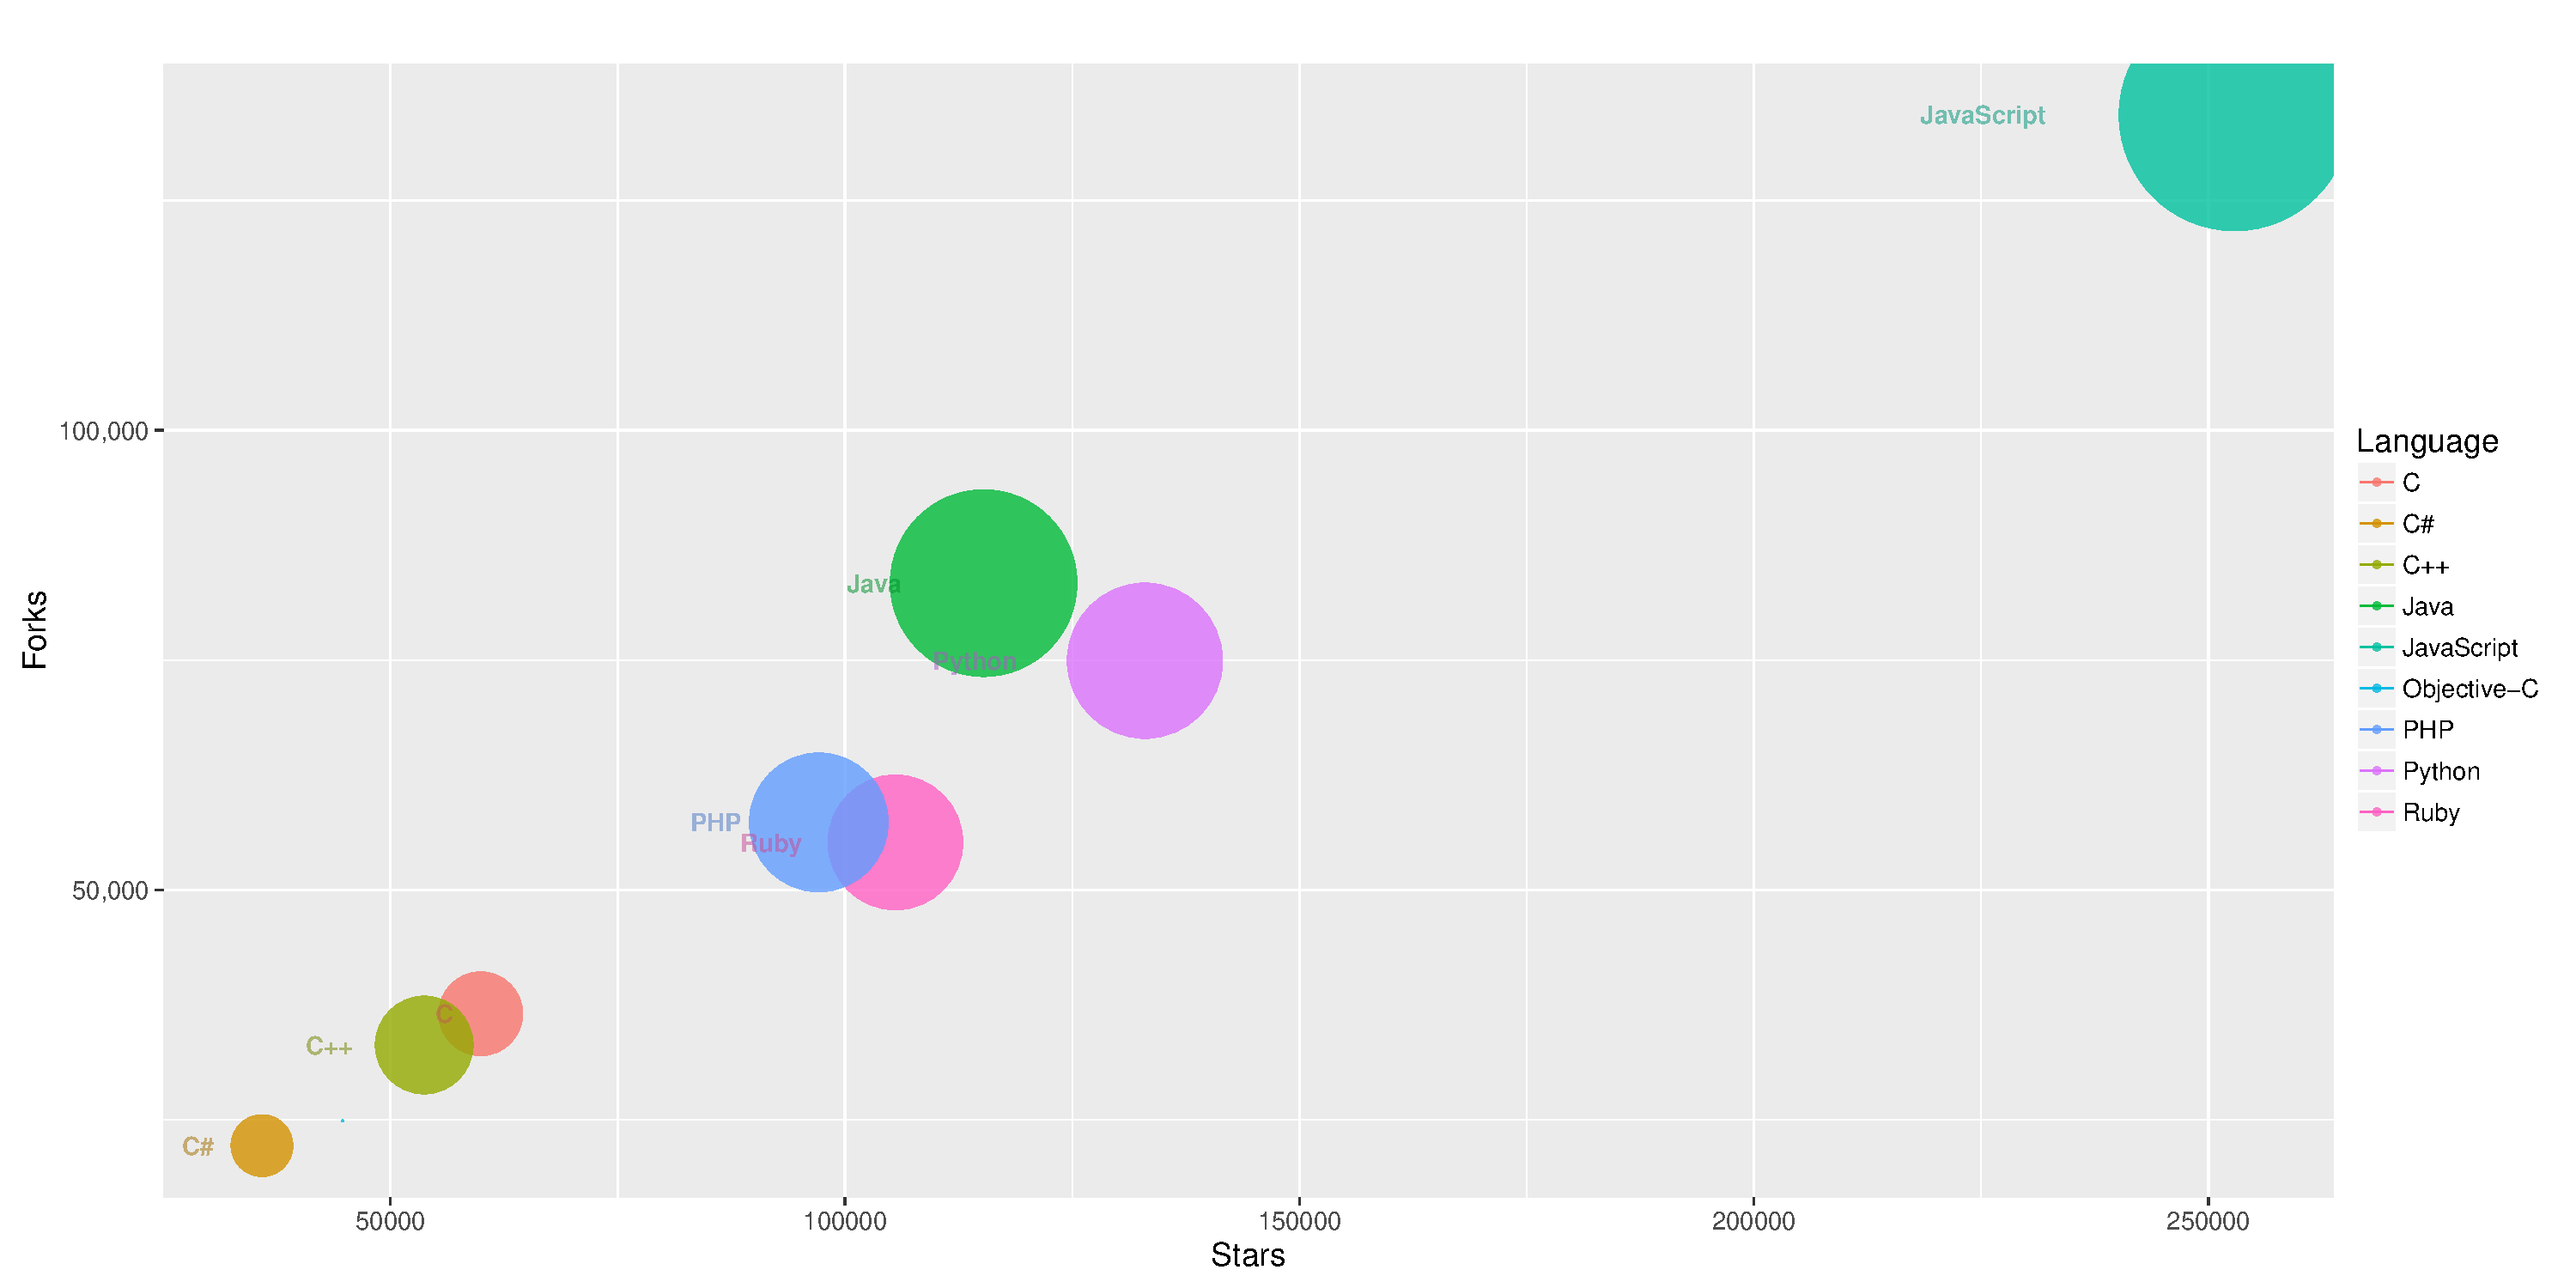
\includegraphics[page=1,scale=0.35]{../graphics/intro/popular_programming_languages.pdf}
	\caption[]{ Most popular languages on GitHub in 2014. The cumulated numbers of forks and stars on all projects can be regarded as proxy for the popularity of the programming language. The size of the circles represents the number of existing projects (proportions: JavaScript contains 323,938 projects, C\# contains 56,062 projects) \footnotemark}
	\label{fig:github_popular_programming_languages}
\end{figure}

\footnotetext{Data origin: \url{http://githut.info/}}

\begin{figure}[h]
	\centering
	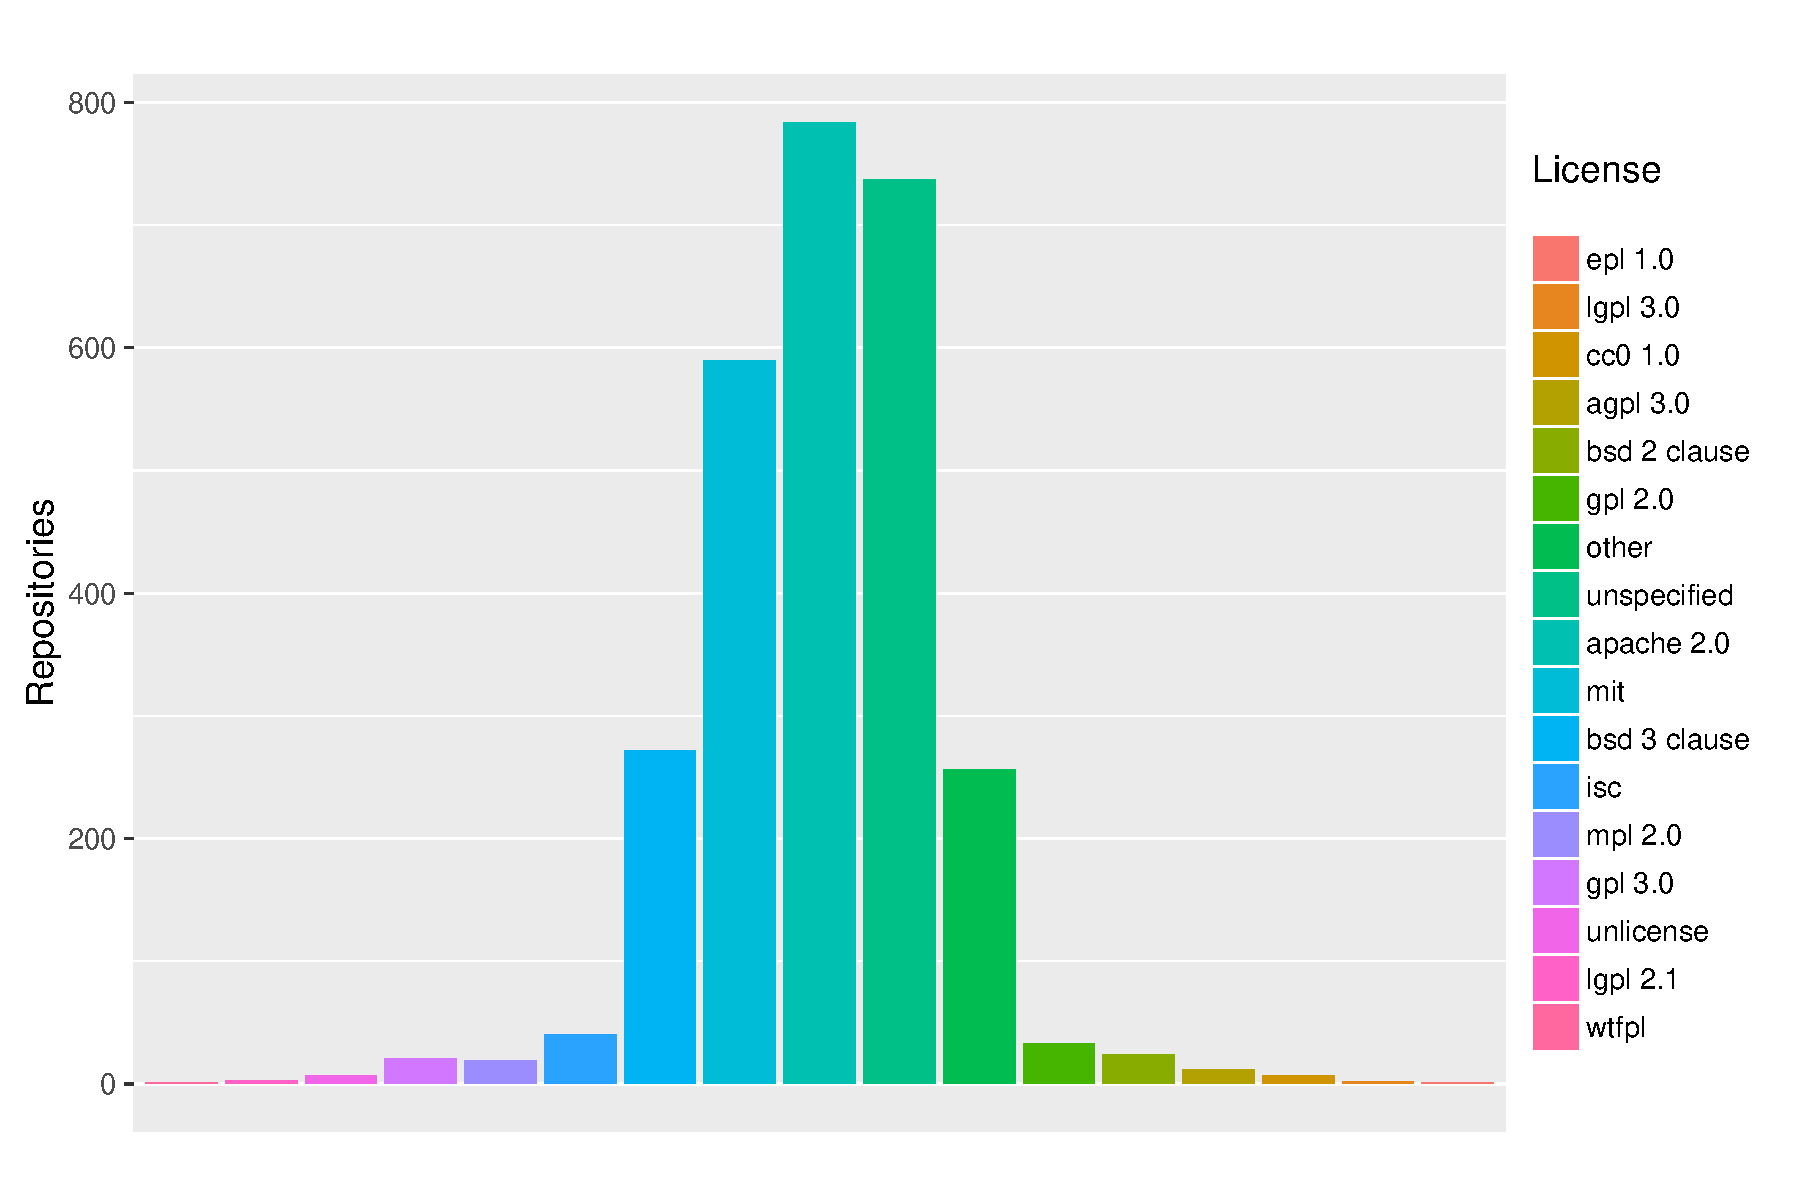
\includegraphics[page=1,scale=0.35]{../graphics/intro/licenses/popular_licenses_residual.pdf}
	\caption{License distribution of firm's residual projects on GitHub.}
	\label{fig:licenses_in_residual_projects}
\end{figure}

\begin{figure}[h]
	\centering
	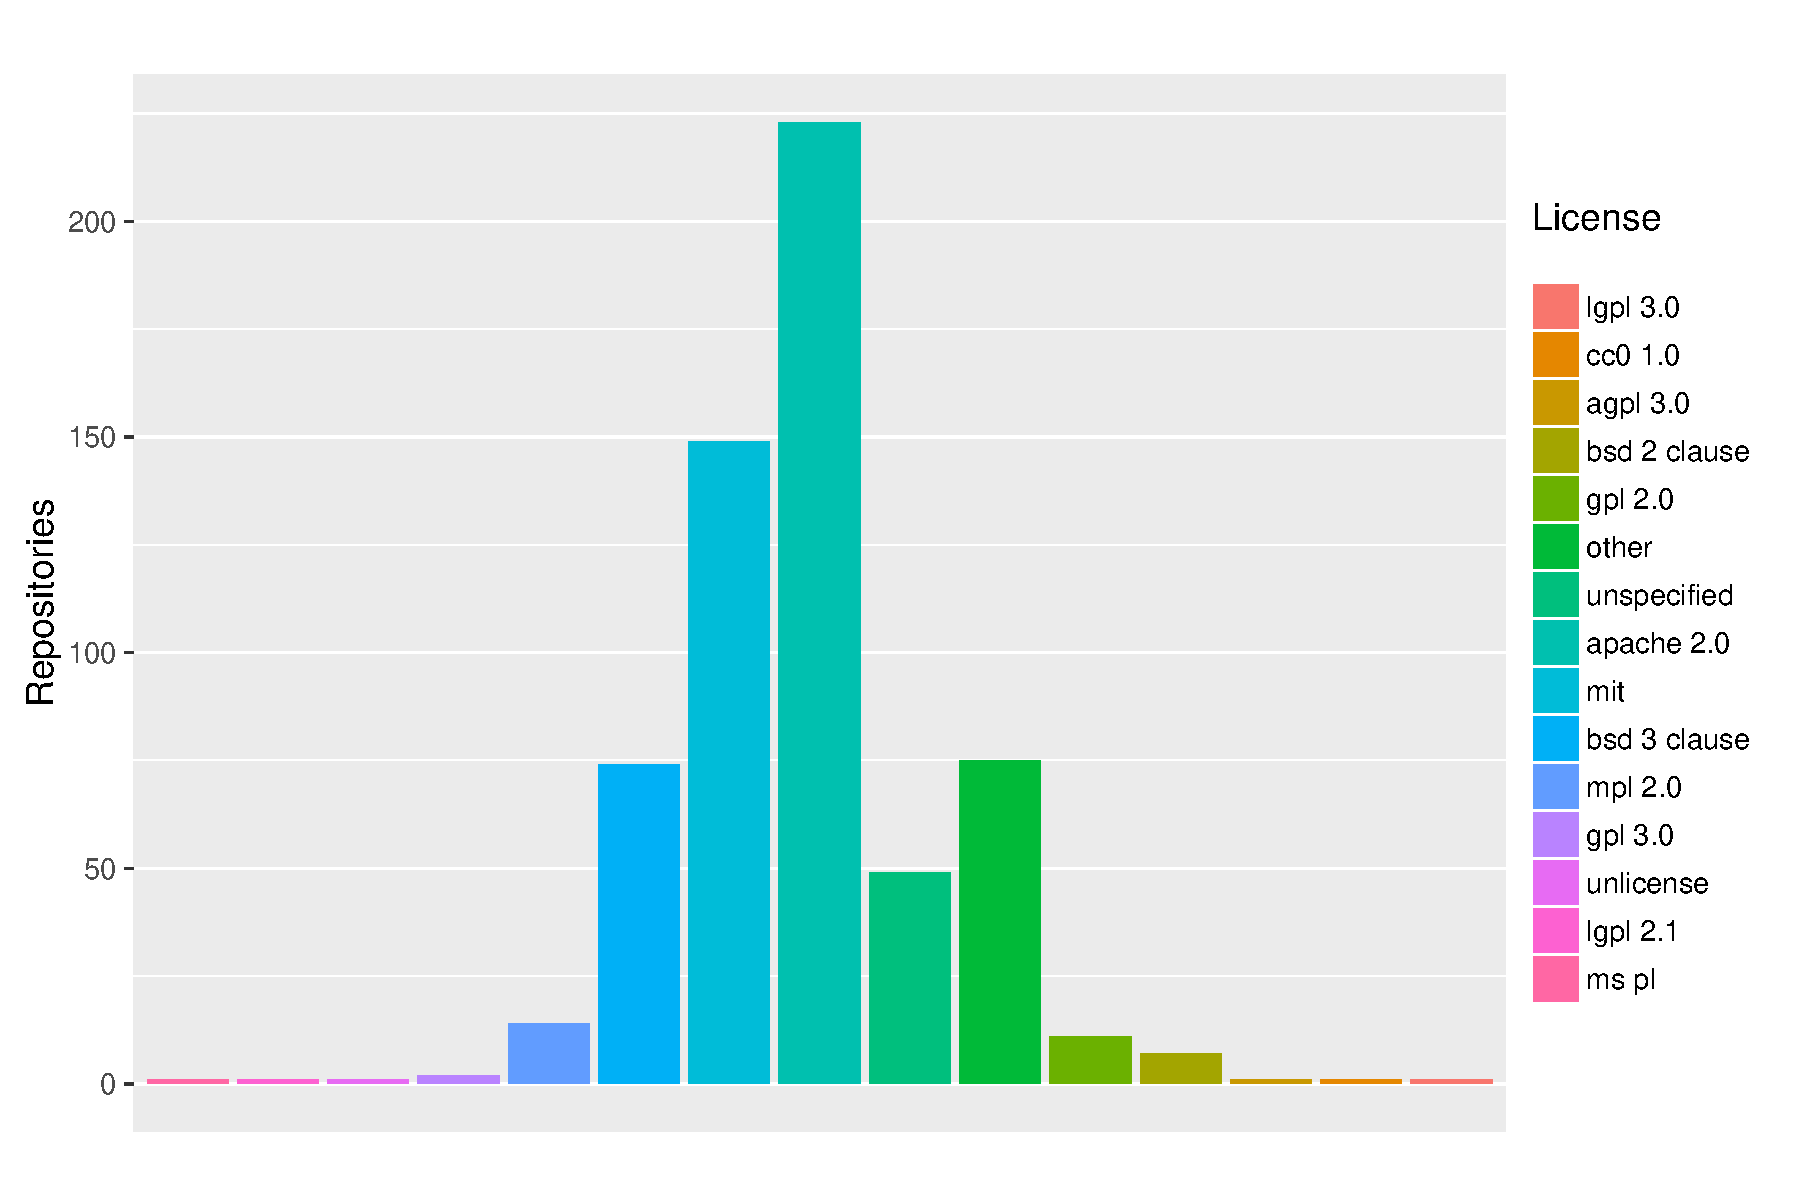
\includegraphics[page=1,scale=0.35]{../graphics/intro/licenses/popular_licenses_top.pdf}
	\caption{License distribution of firm's top projects on GitHub.}
	\label{fig:licenses_in_top_projects}
\end{figure}

\clearpage
\subsection{Plots of Code Contribution}

\begin{figure}[!ht]
	\centering
	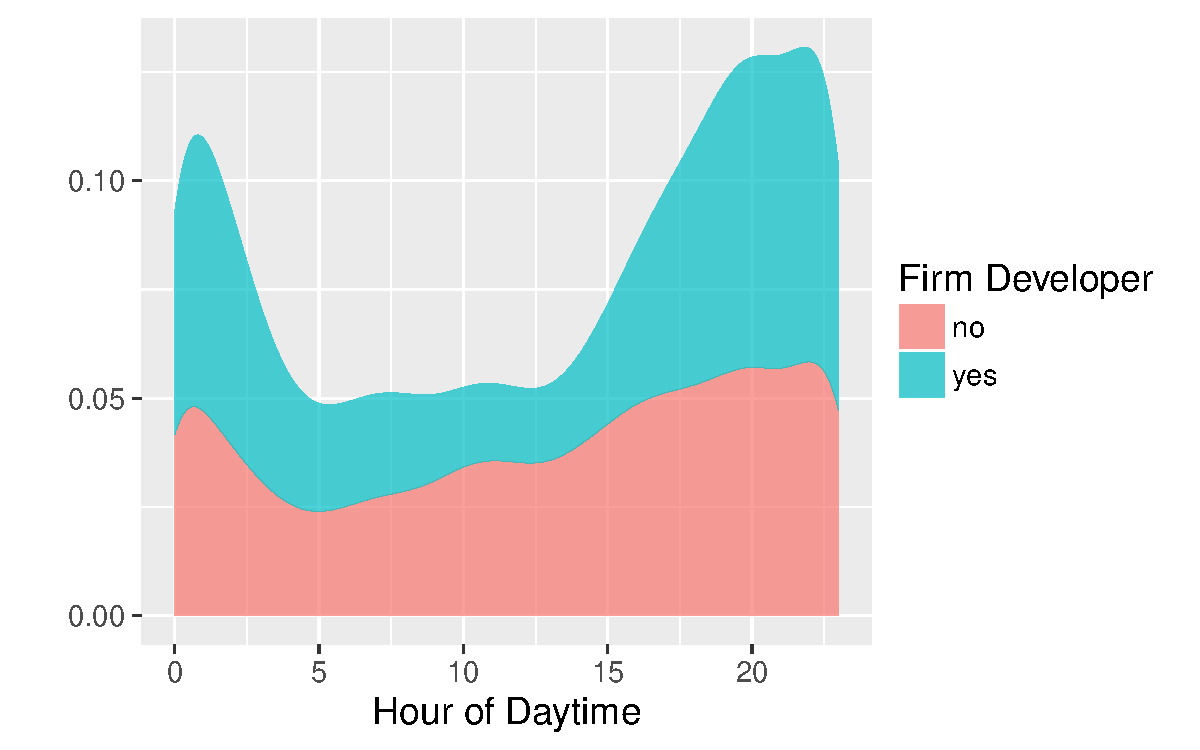
\includegraphics[page=1,scale=0.7]{../graphics/intro/hour_of_code_contribution_daytime_worldtime.pdf}
	\caption{Code contributions by firm employed and external developers based on worldwide consideration (UTC time). Most commits are placed during the late evening which is between morning and midday (9:00 - 16:00) in California, USA (UTC -8)}
	\label{fig:distribution_developer_commits_wordlwide}
\end{figure}

\begin{figure}[!ht]
	\centering
	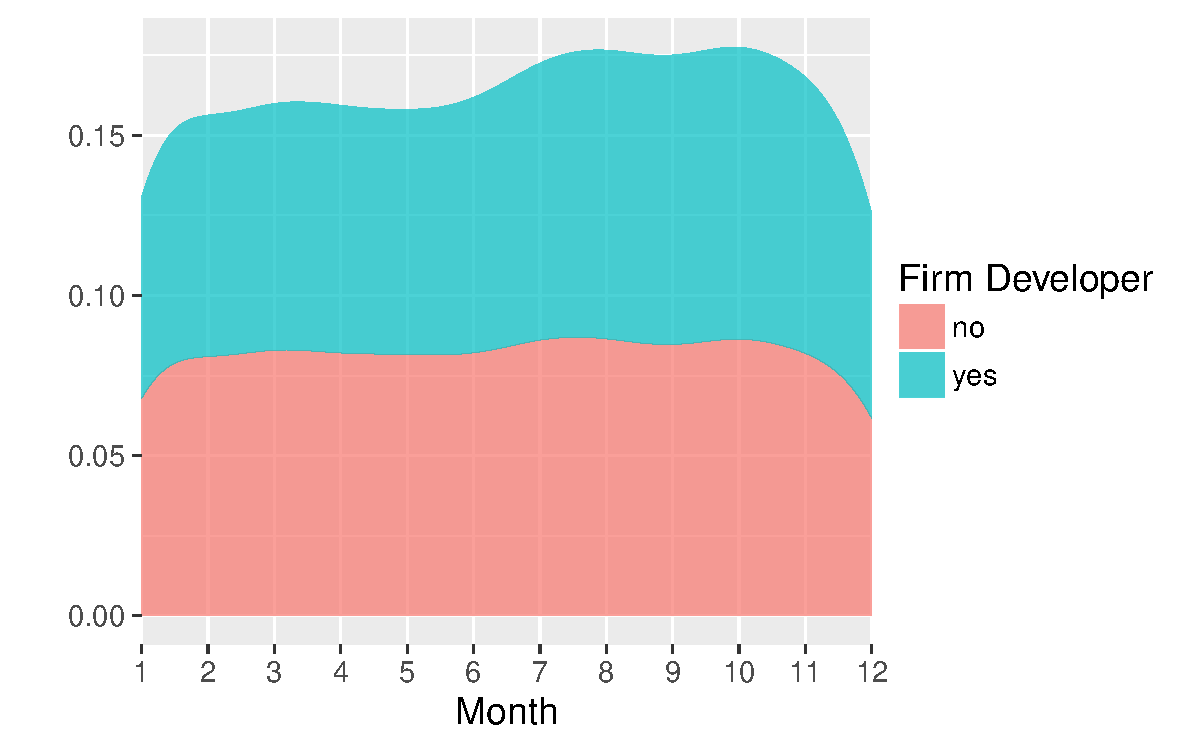
\includegraphics[page=1,scale=0.7]{../graphics/intro/month_of_code_contribution.pdf}
	\caption{Code contributions by firm employed and external developers over the year (January - December)}
	\label{fig:distribution_developer_commits_by_month}
\end{figure}

\subsection{Plots of Repositories}

\begin{figure}[h]
	\centering
	\label{fig:stars_contributors}
	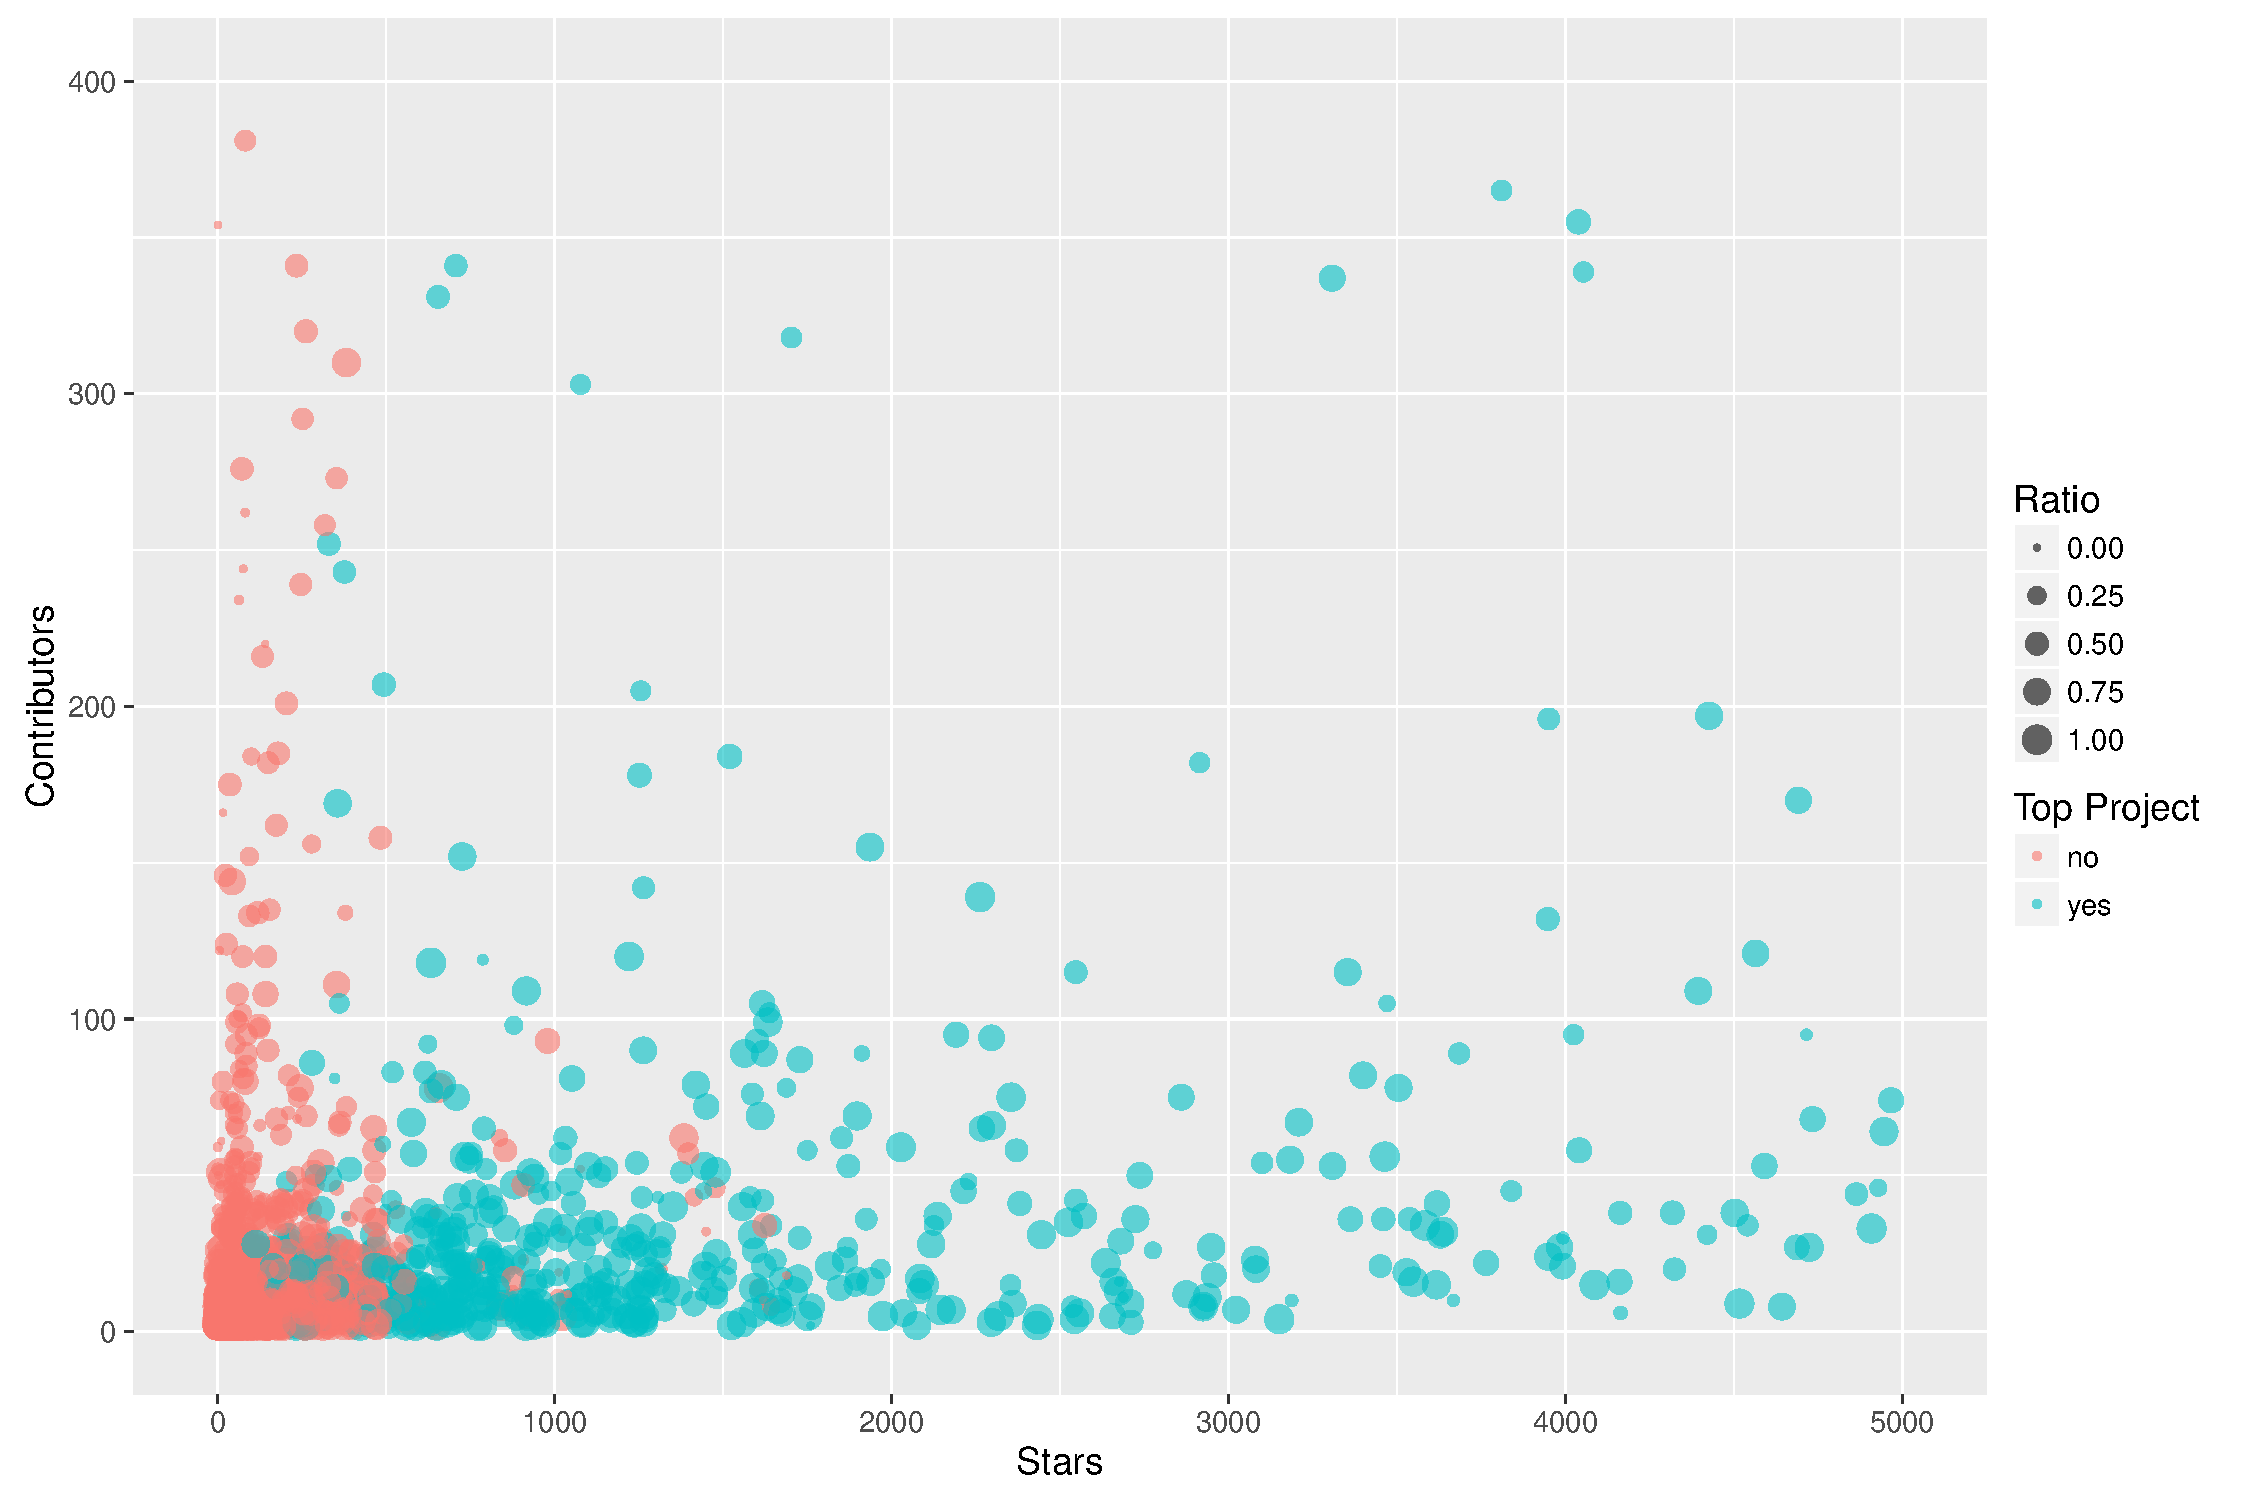
\includegraphics[page=1,scale=0.35]{../graphics/intro/stars_contributors.pdf}
	\caption{The "ratio" (code commitment share of firm employed developers), represented by size of dots, is quite high on all observed projects ($\geq 0.5$)}
\end{figure}

\begin{figure}[h]
	\centering
	\label{fig:stars_contributors_low_ratio_projects}
	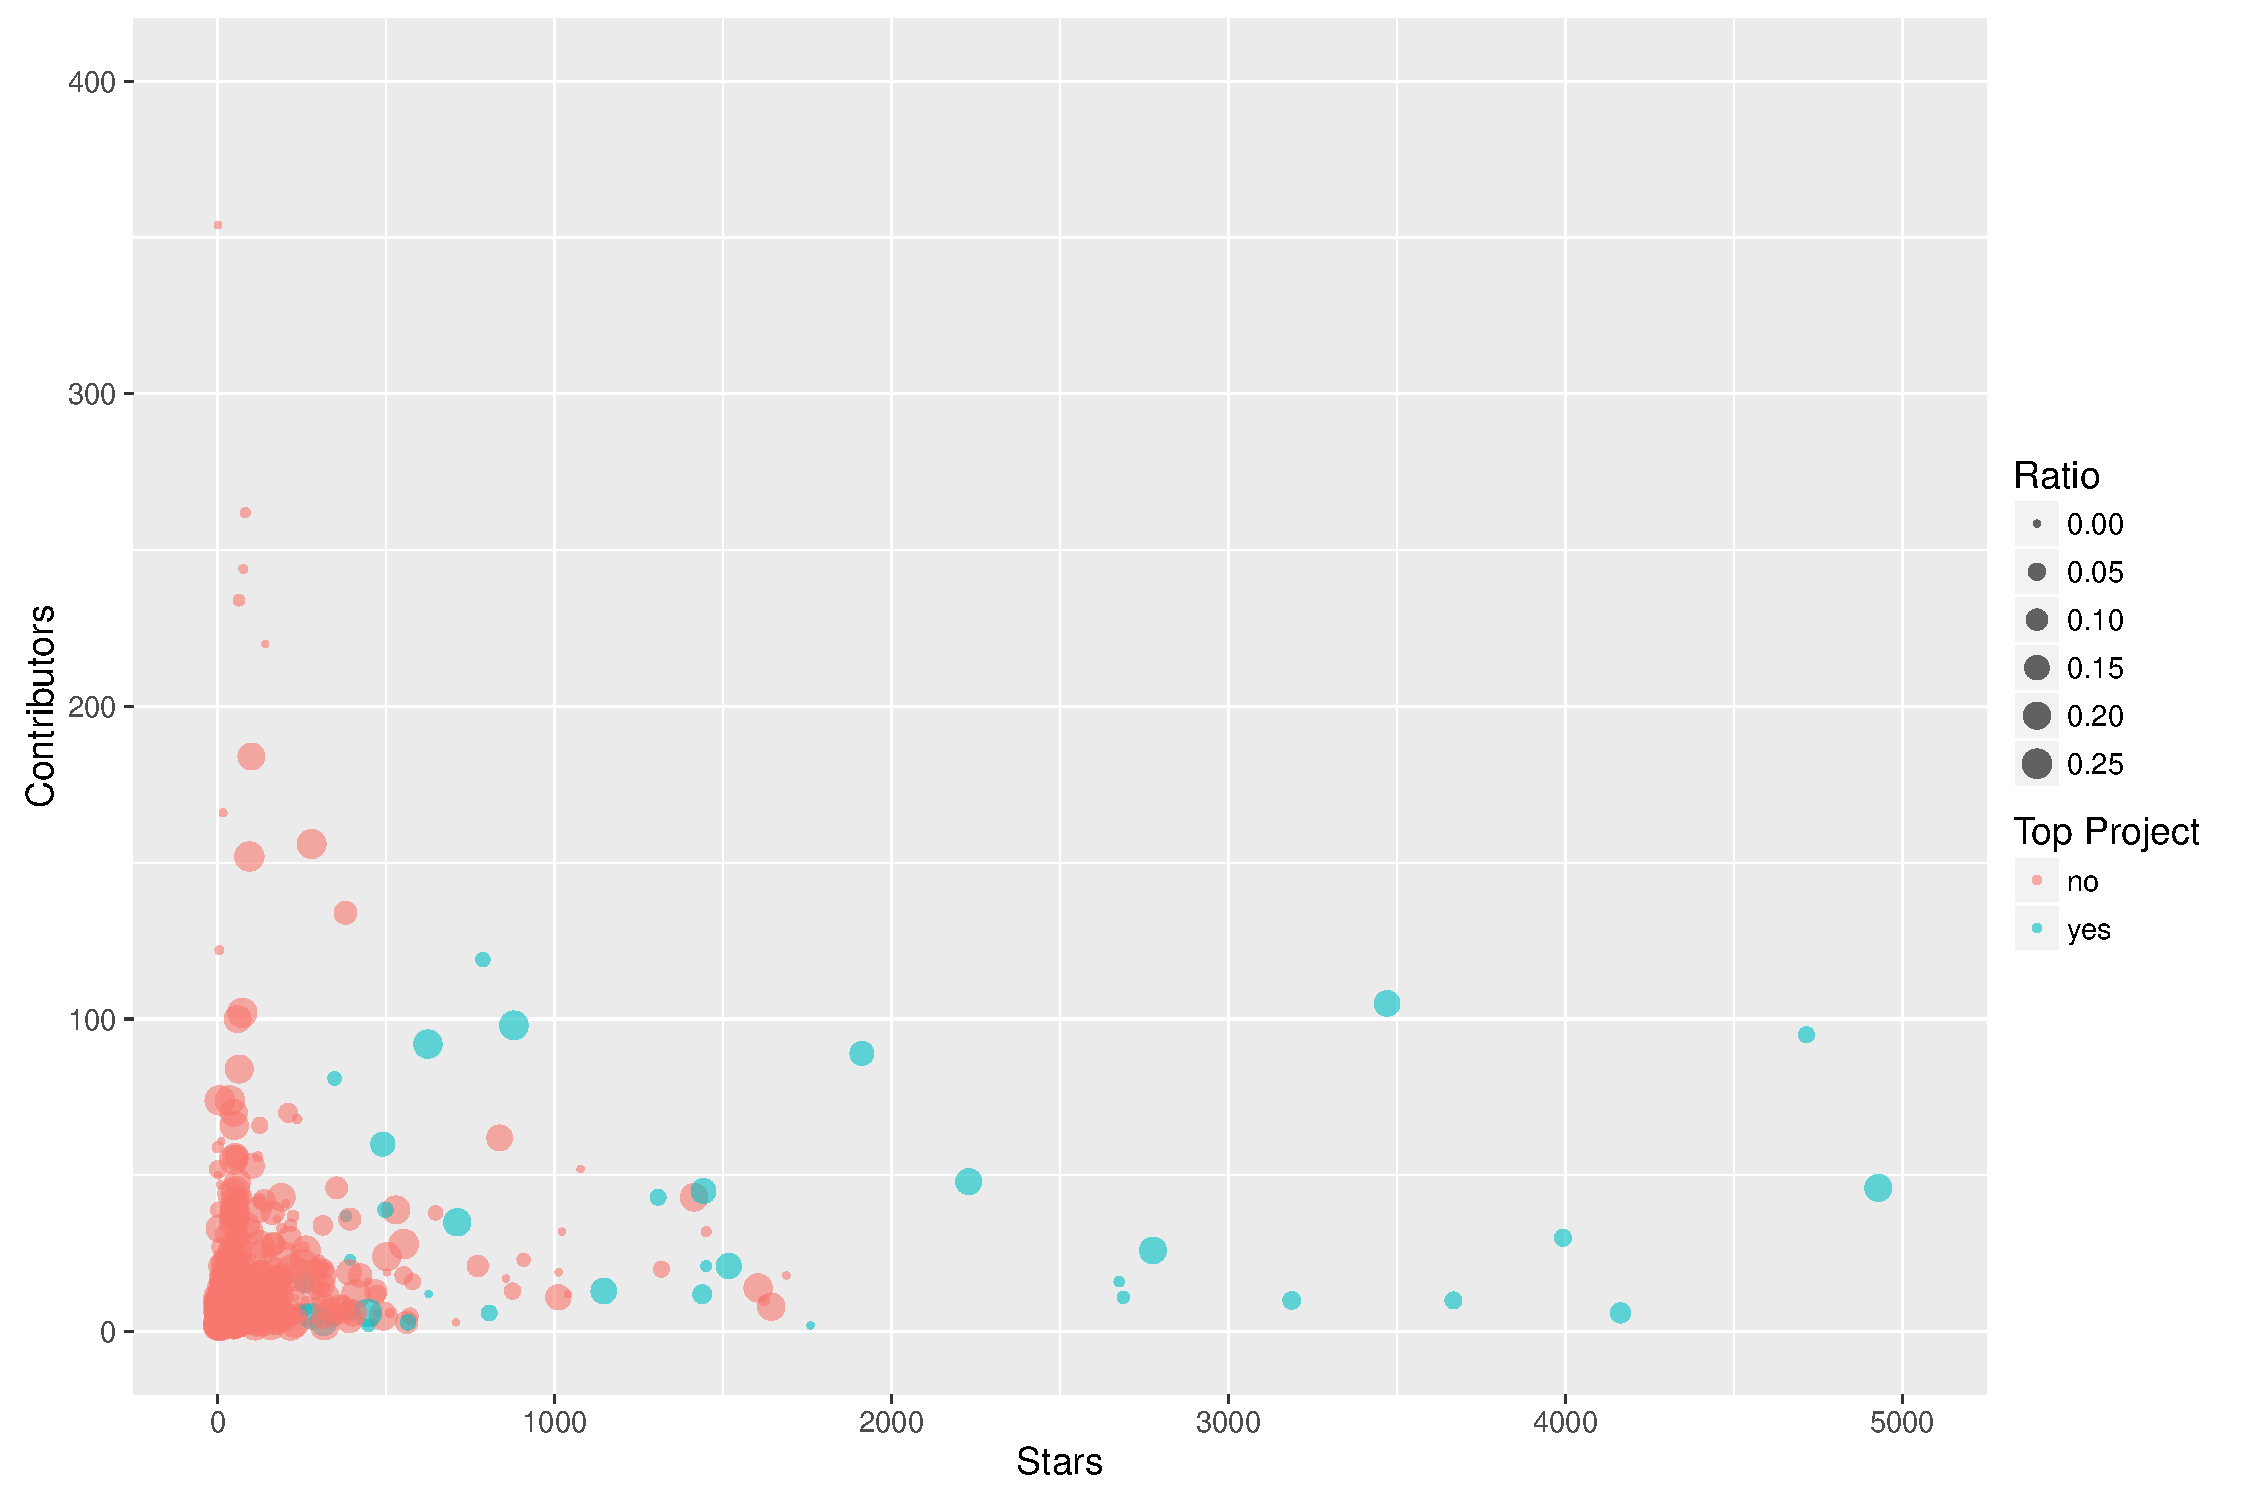
\includegraphics[page=1,scale=0.35]{../graphics/intro/stars_contributors_low_ratio_projects.pdf}
	\caption{If the ratio is low ($\leq 0.25$) there are fewer top projects / less stargazers}
\end{figure}

\begin{figure}
	\centering
	\label{fig:stars_contributors_high_ratio_projects}
	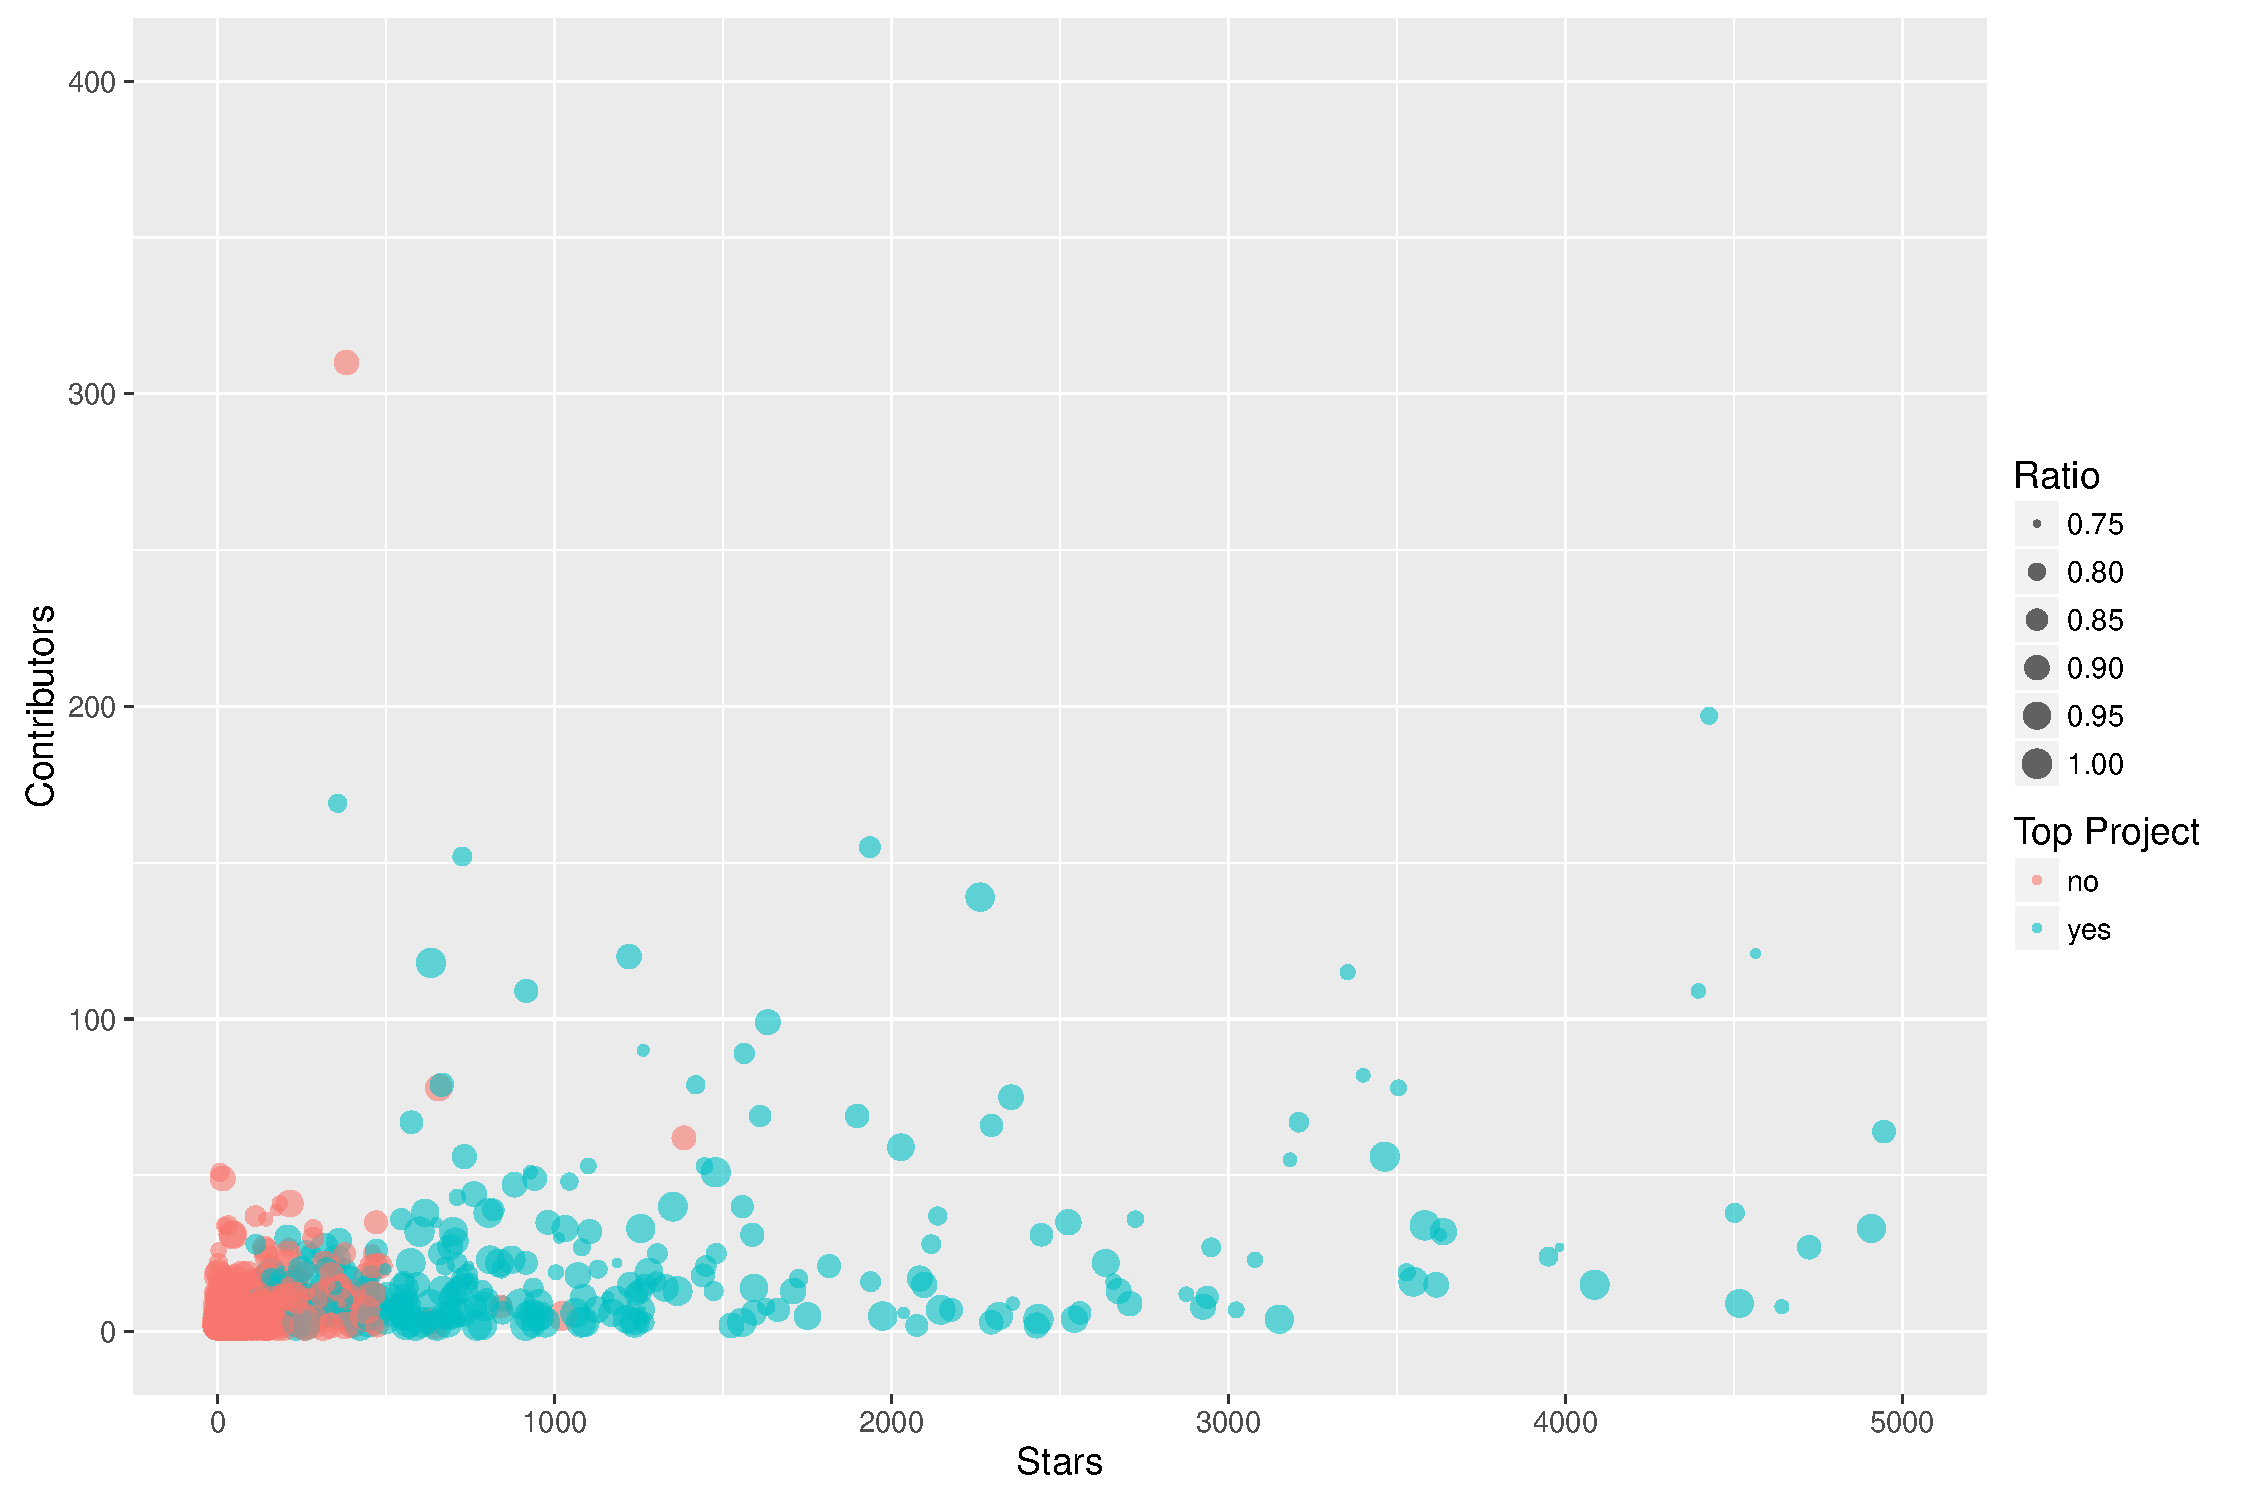
\includegraphics[page=1,scale=0.4]{../graphics/intro/stars_contributors_high_ratio_projects.pdf}
	\caption{If the ratio is higher ($\geq 0.75$) there are more top projects / stargazers}
\end{figure}

\begin{landscape}
\begin{figure}
	\centering
	\label{fig:code_contribution_age_ratio}
	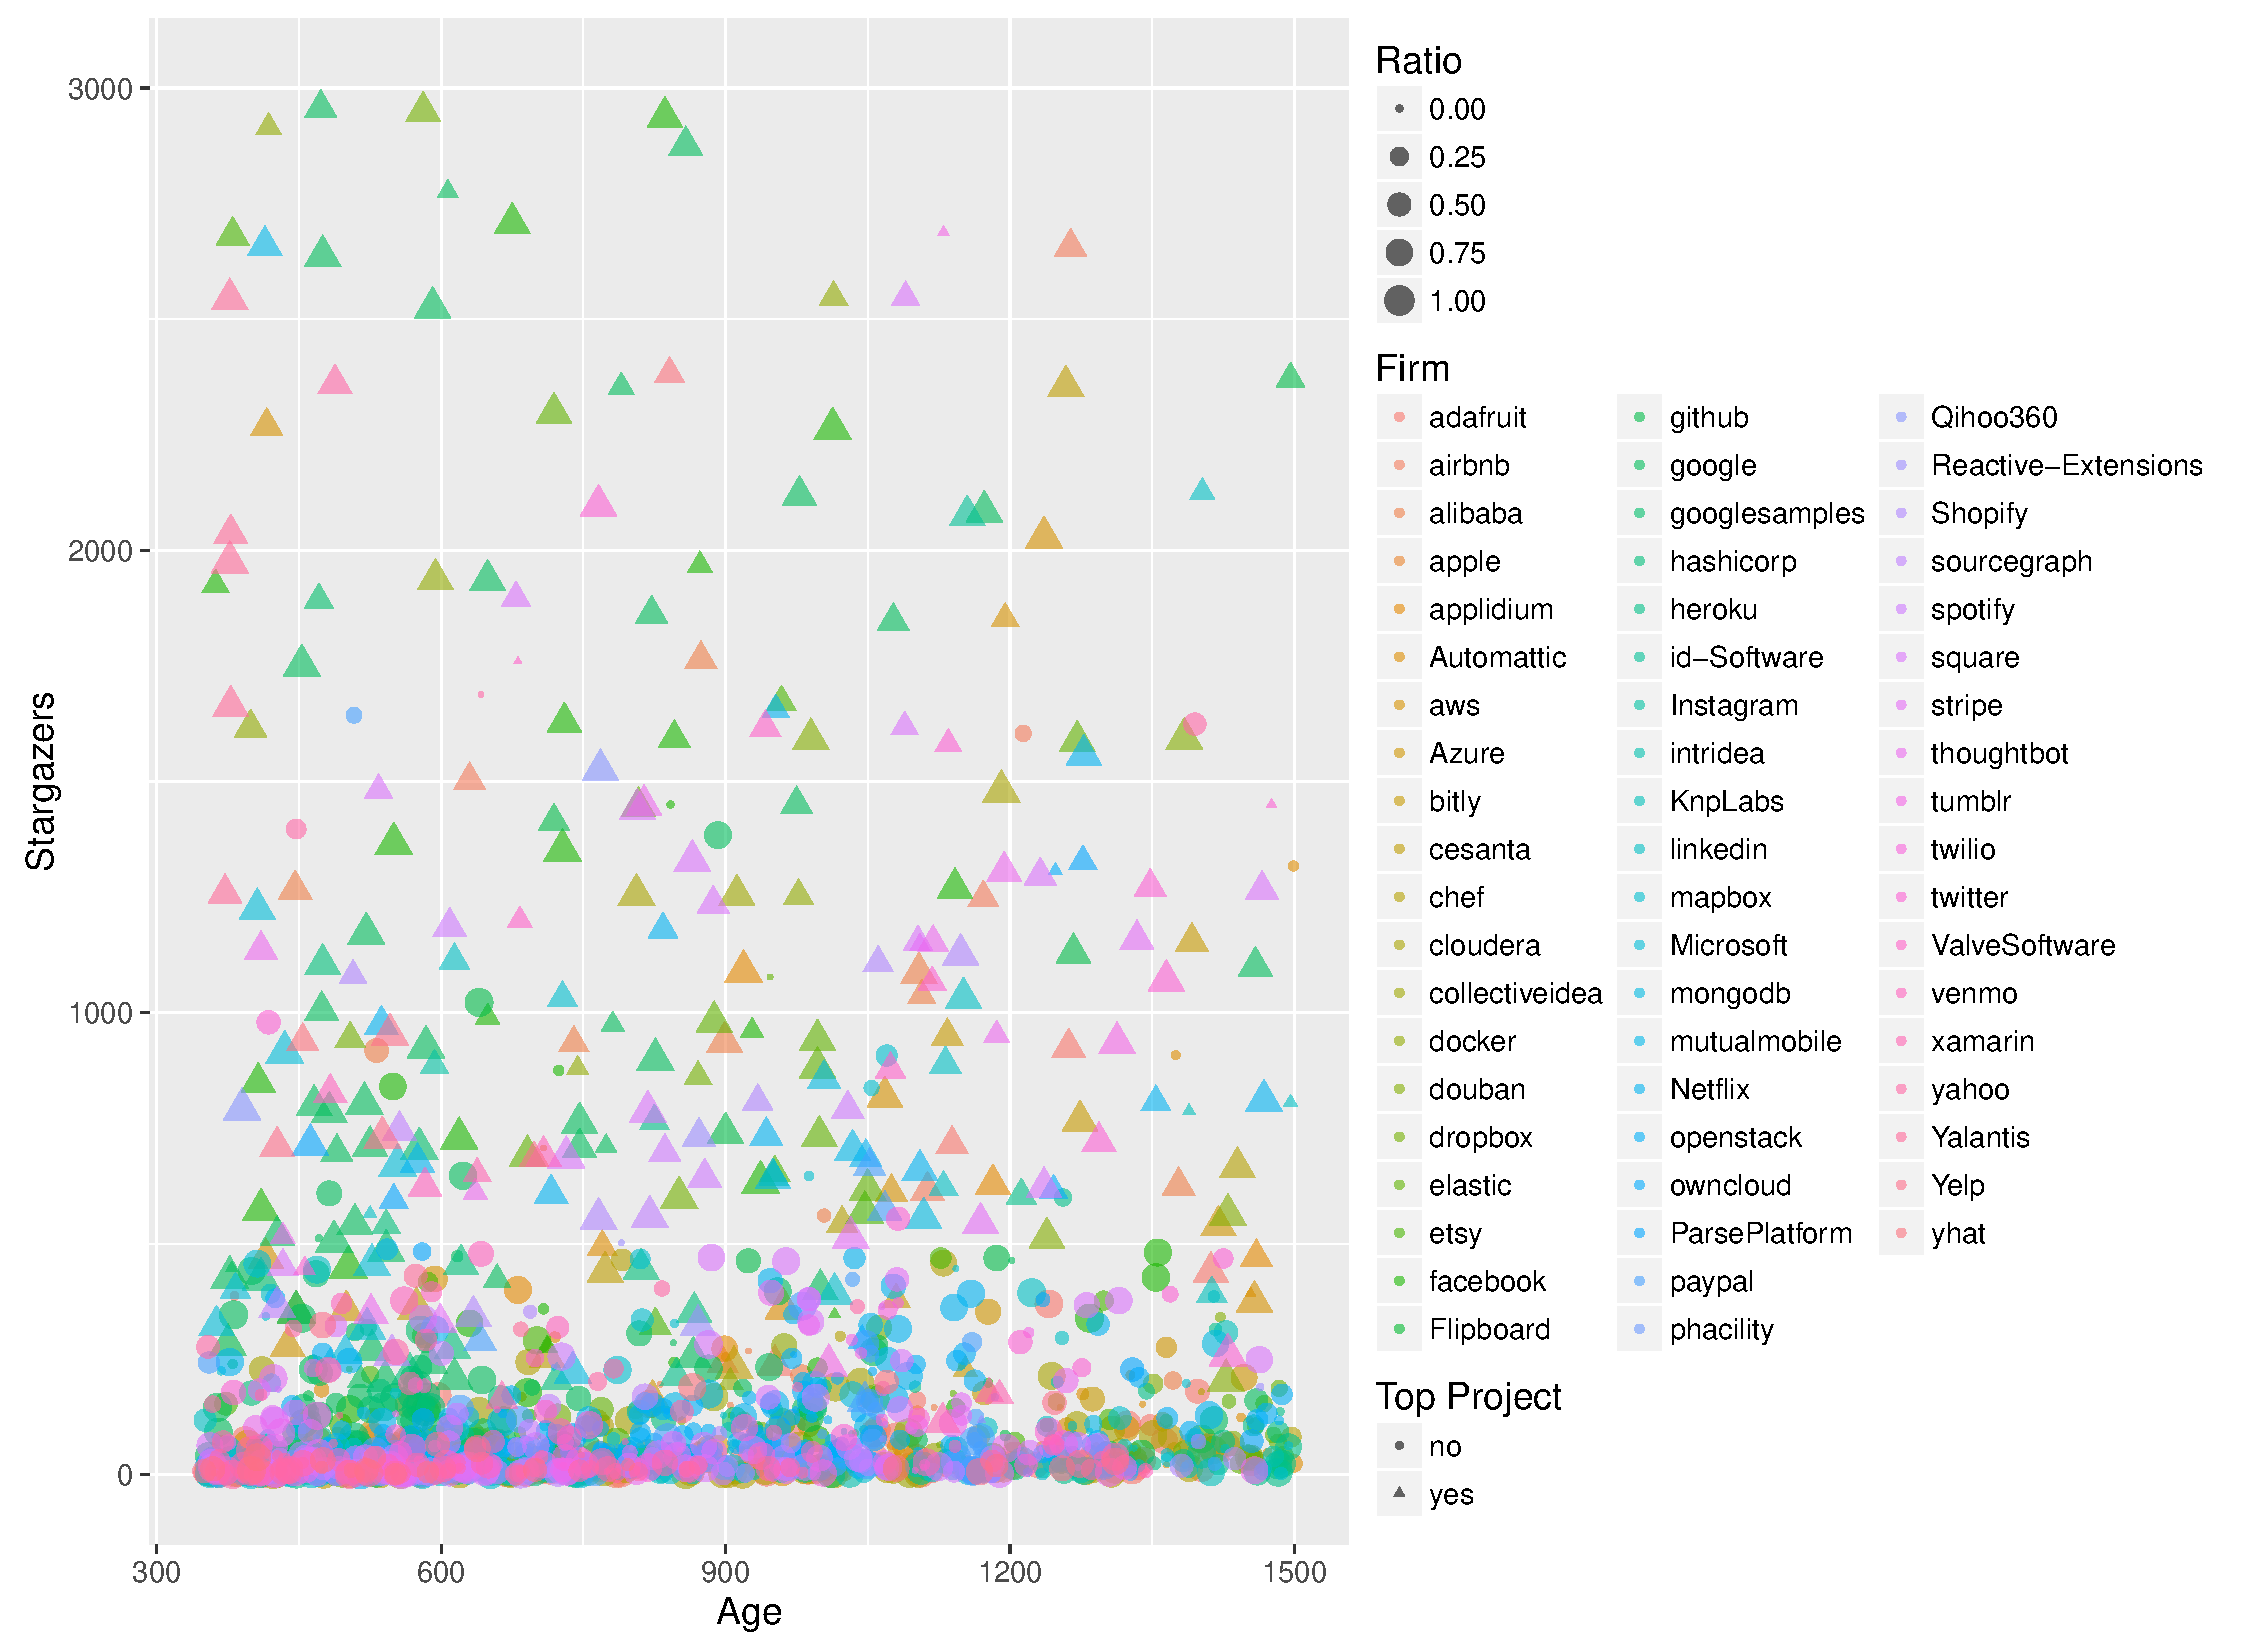
\includegraphics[page=1,scale=0.45]{../graphics/intro/code_contribution_age_ratio.pdf}
	\caption{The age of projects (in days), their popularity (number of stars), colored by firms, size of shapes by "ratio" (code commitment share of firm employed developers) and shape by "Top Project" or "Residual Project". All plotted projects are less than 4.5 years old.}
\end{figure}

\begin{figure}
	\centering
	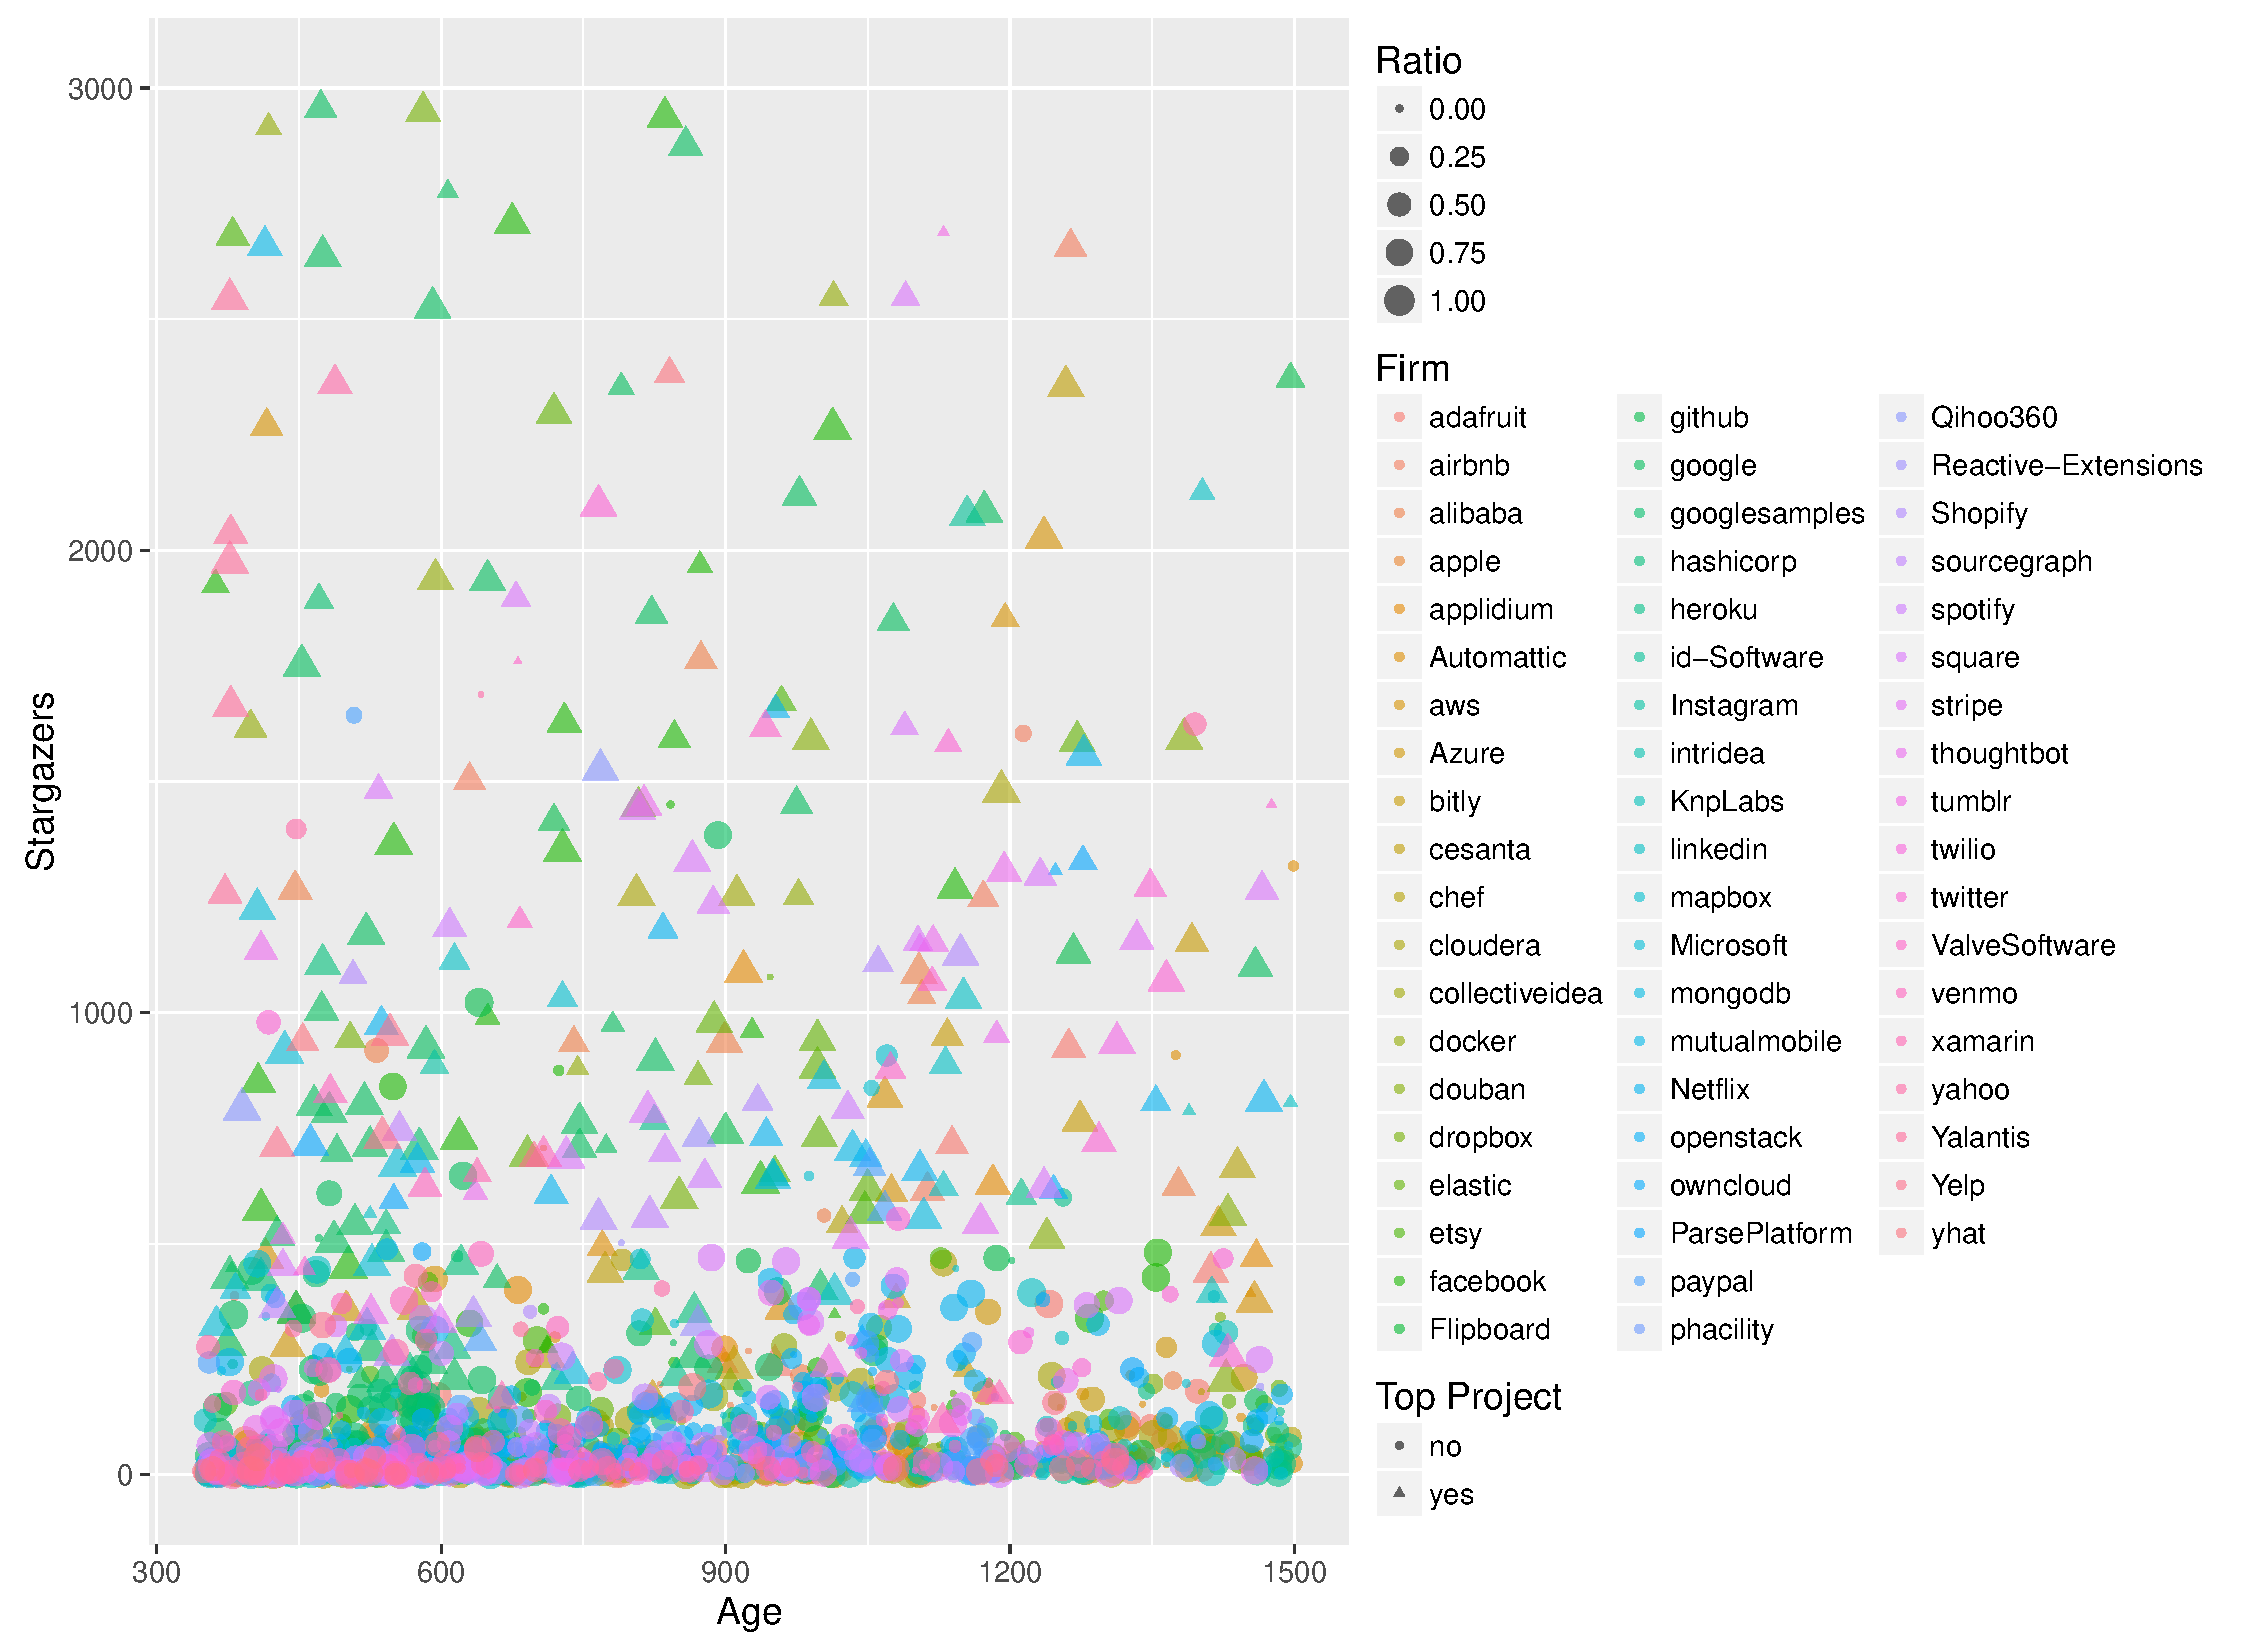
\includegraphics[page=1,scale=0.45]{../graphics/intro/code_contribution_age_ratio.pdf}
	\caption{The age of projects (in days), their popularity (number of stars), colored by (all) firms, size of shapes by "ratio" (code commitment share of firm employed developers) and shape by "Top Project" or "Residual Project". All plotted projects are less than 4.5 years old.}
	\label{fig:code_contribution_age_ratio}
\end{figure}

\begin{figure}
	\centering
	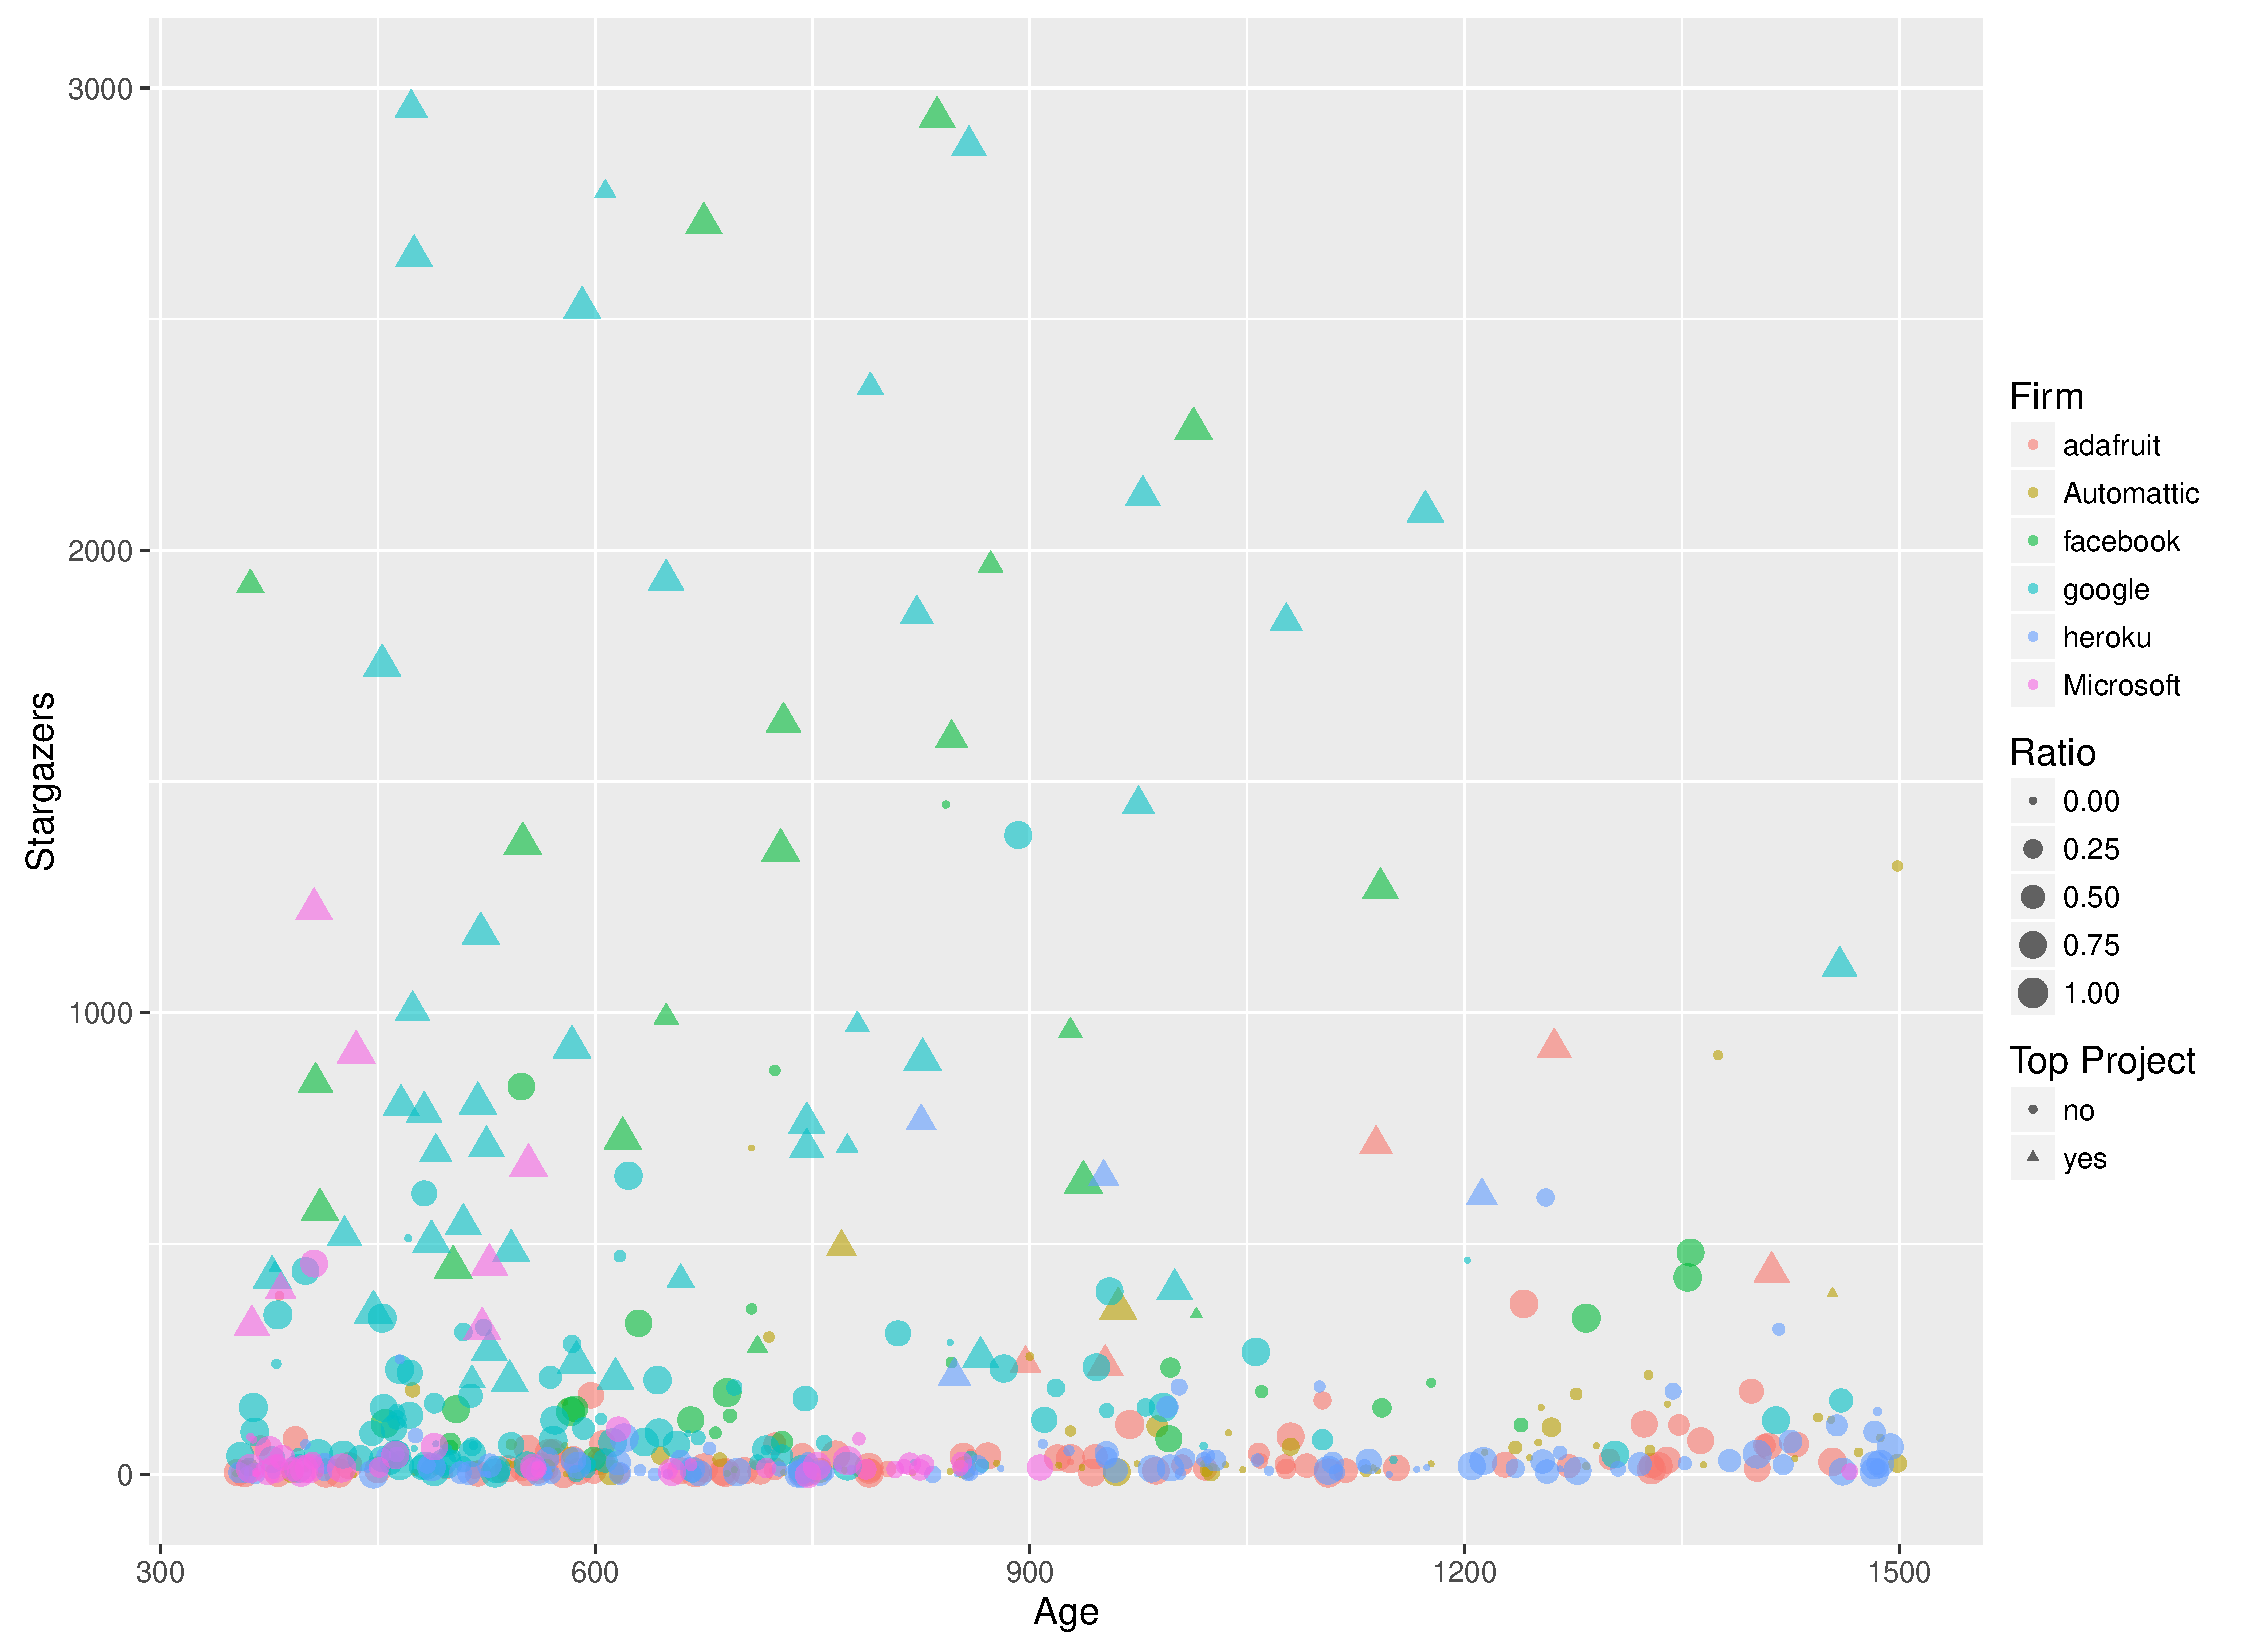
\includegraphics[page=1,scale=0.4]{../graphics/intro/code_contribution_age_firms_ratio.pdf}
	\caption{The age of projects (in days), their popularity (number of stars), colored by firms with most popular OS projects, size of shapes by "ratio" (code commitment share of firm employed developers) and shape by "Top Project" or "Residual Project". All plotted projects are less than 4.5 years old.}
	\label{fig:code_contribution_age_firms_ratio}
\end{figure}

\begin{figure}
	\centering
	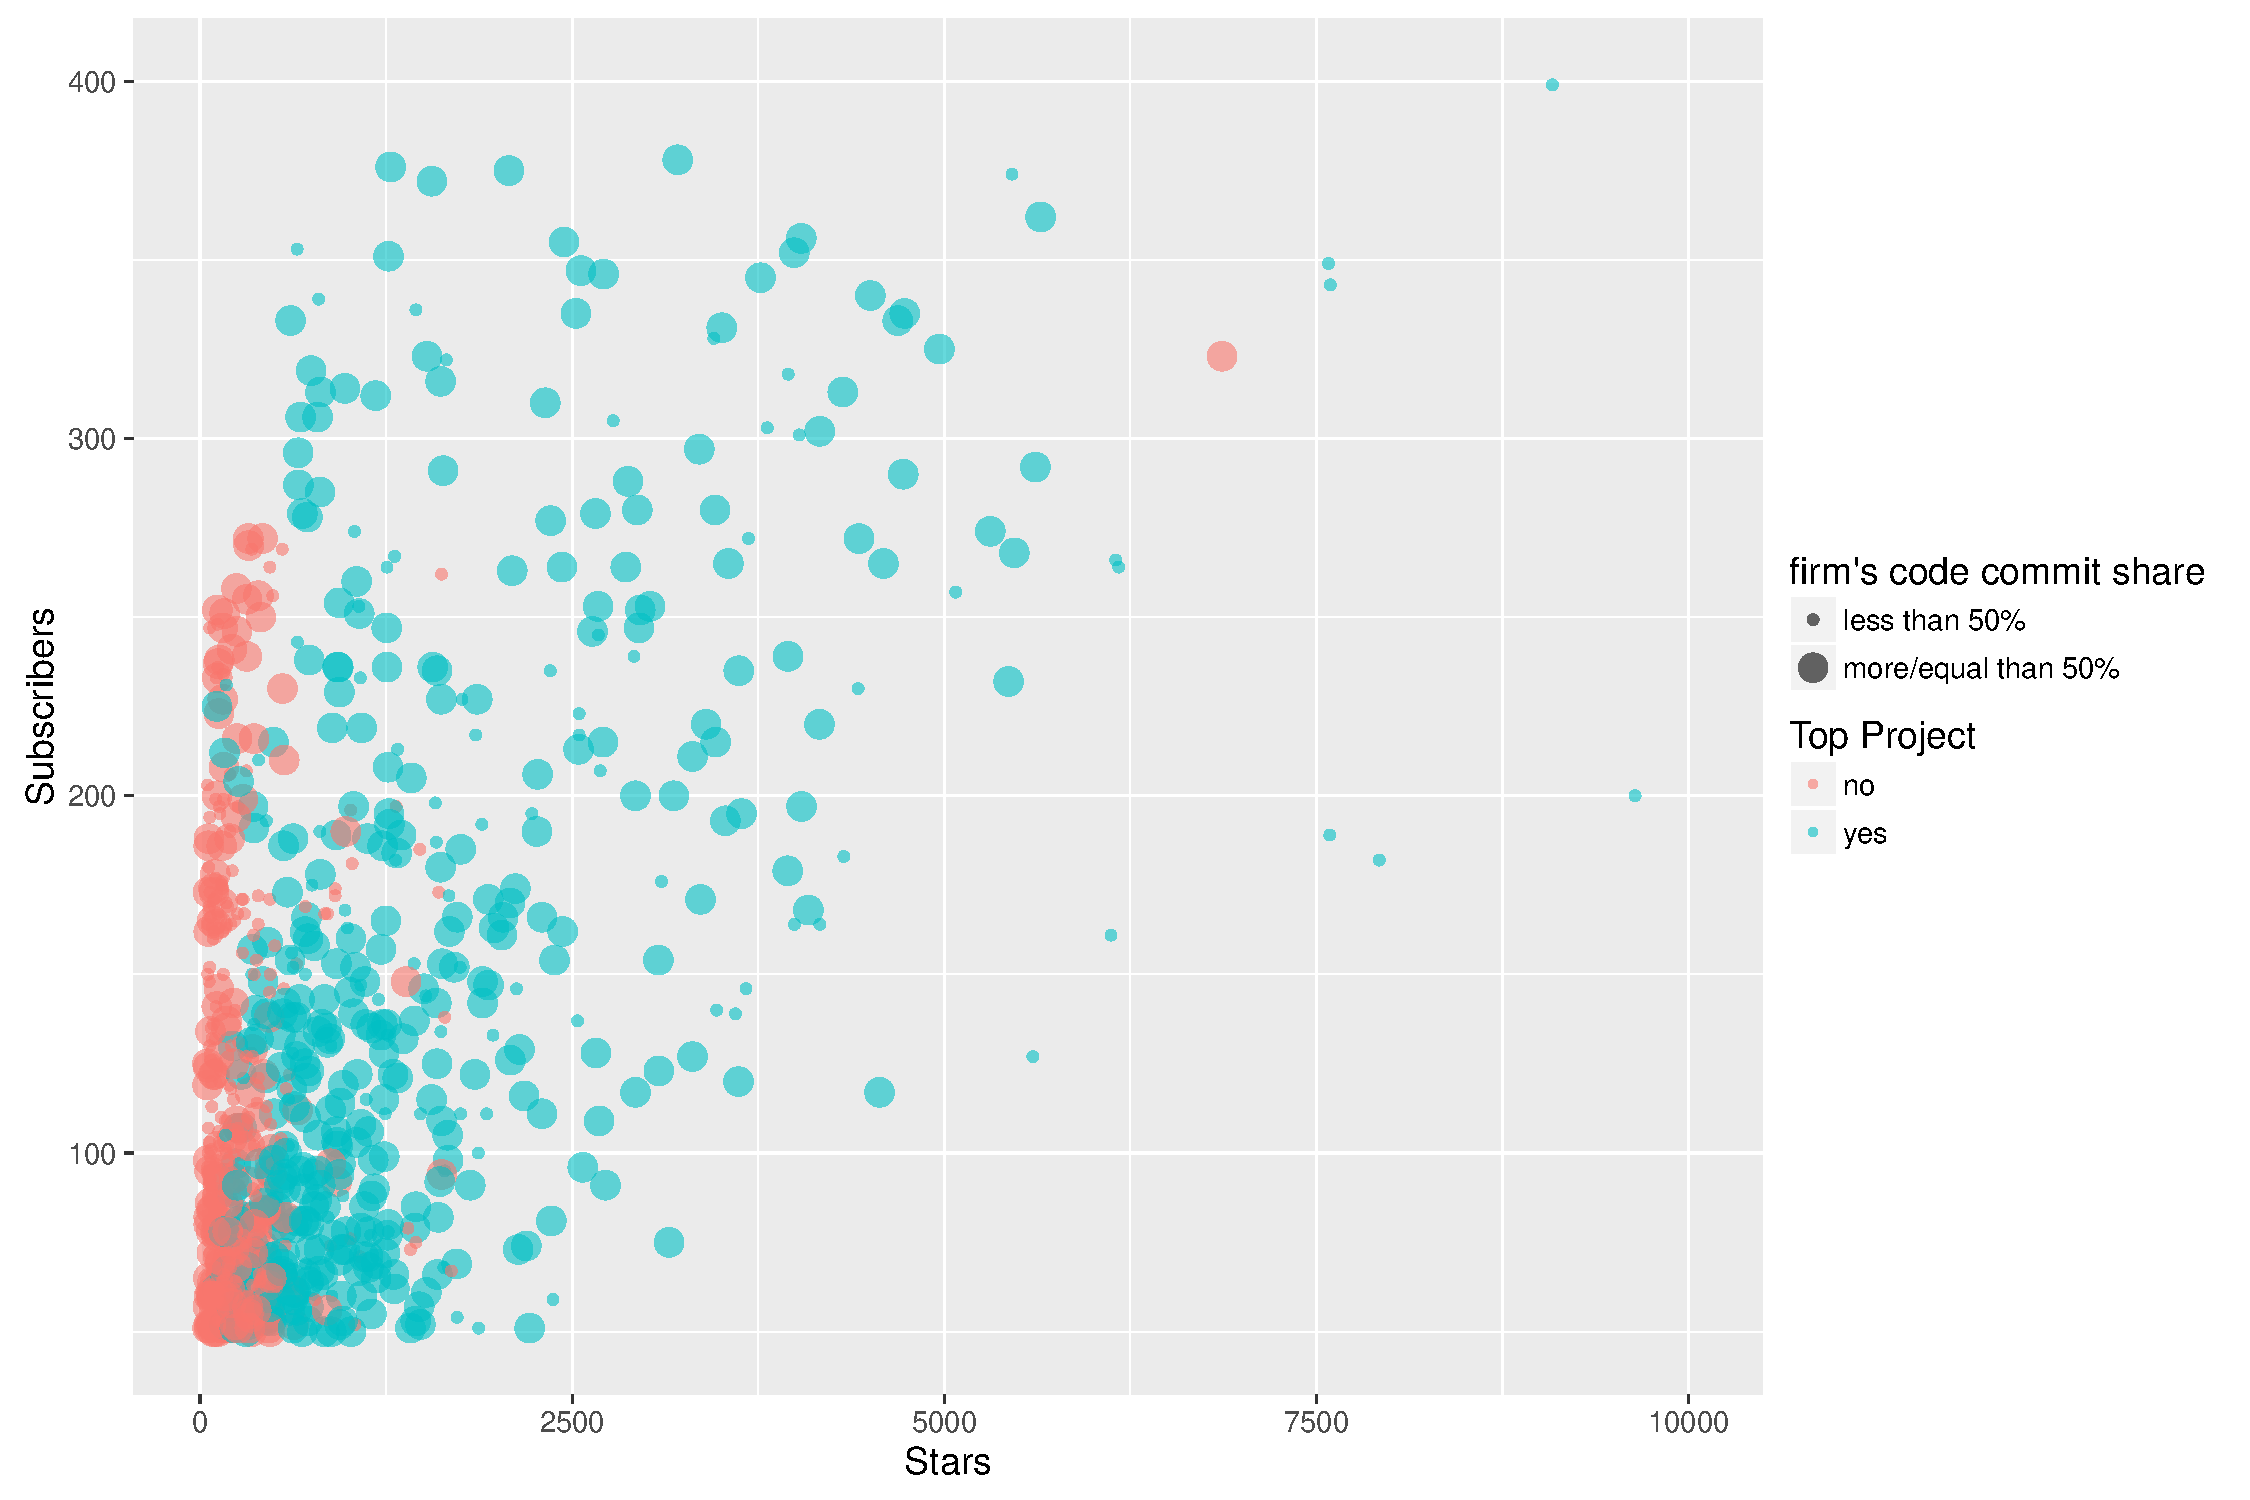
\includegraphics[page=1,scale=0.4]{../graphics/intro/stars_subscribers_ratio_top_10000.pdf}
	\caption{Seperation in ratio $< 0.5$ and $\geq 0.5$; Plotted with Stars against Subscribers (proxies for popularity), colored in Top and Residual Projects and scaled x-axis up to 10,000 stars.}
	\label{fig:stars_subscribers_ratio_top_10000}
\end{figure}

\begin{figure}
	\centering
	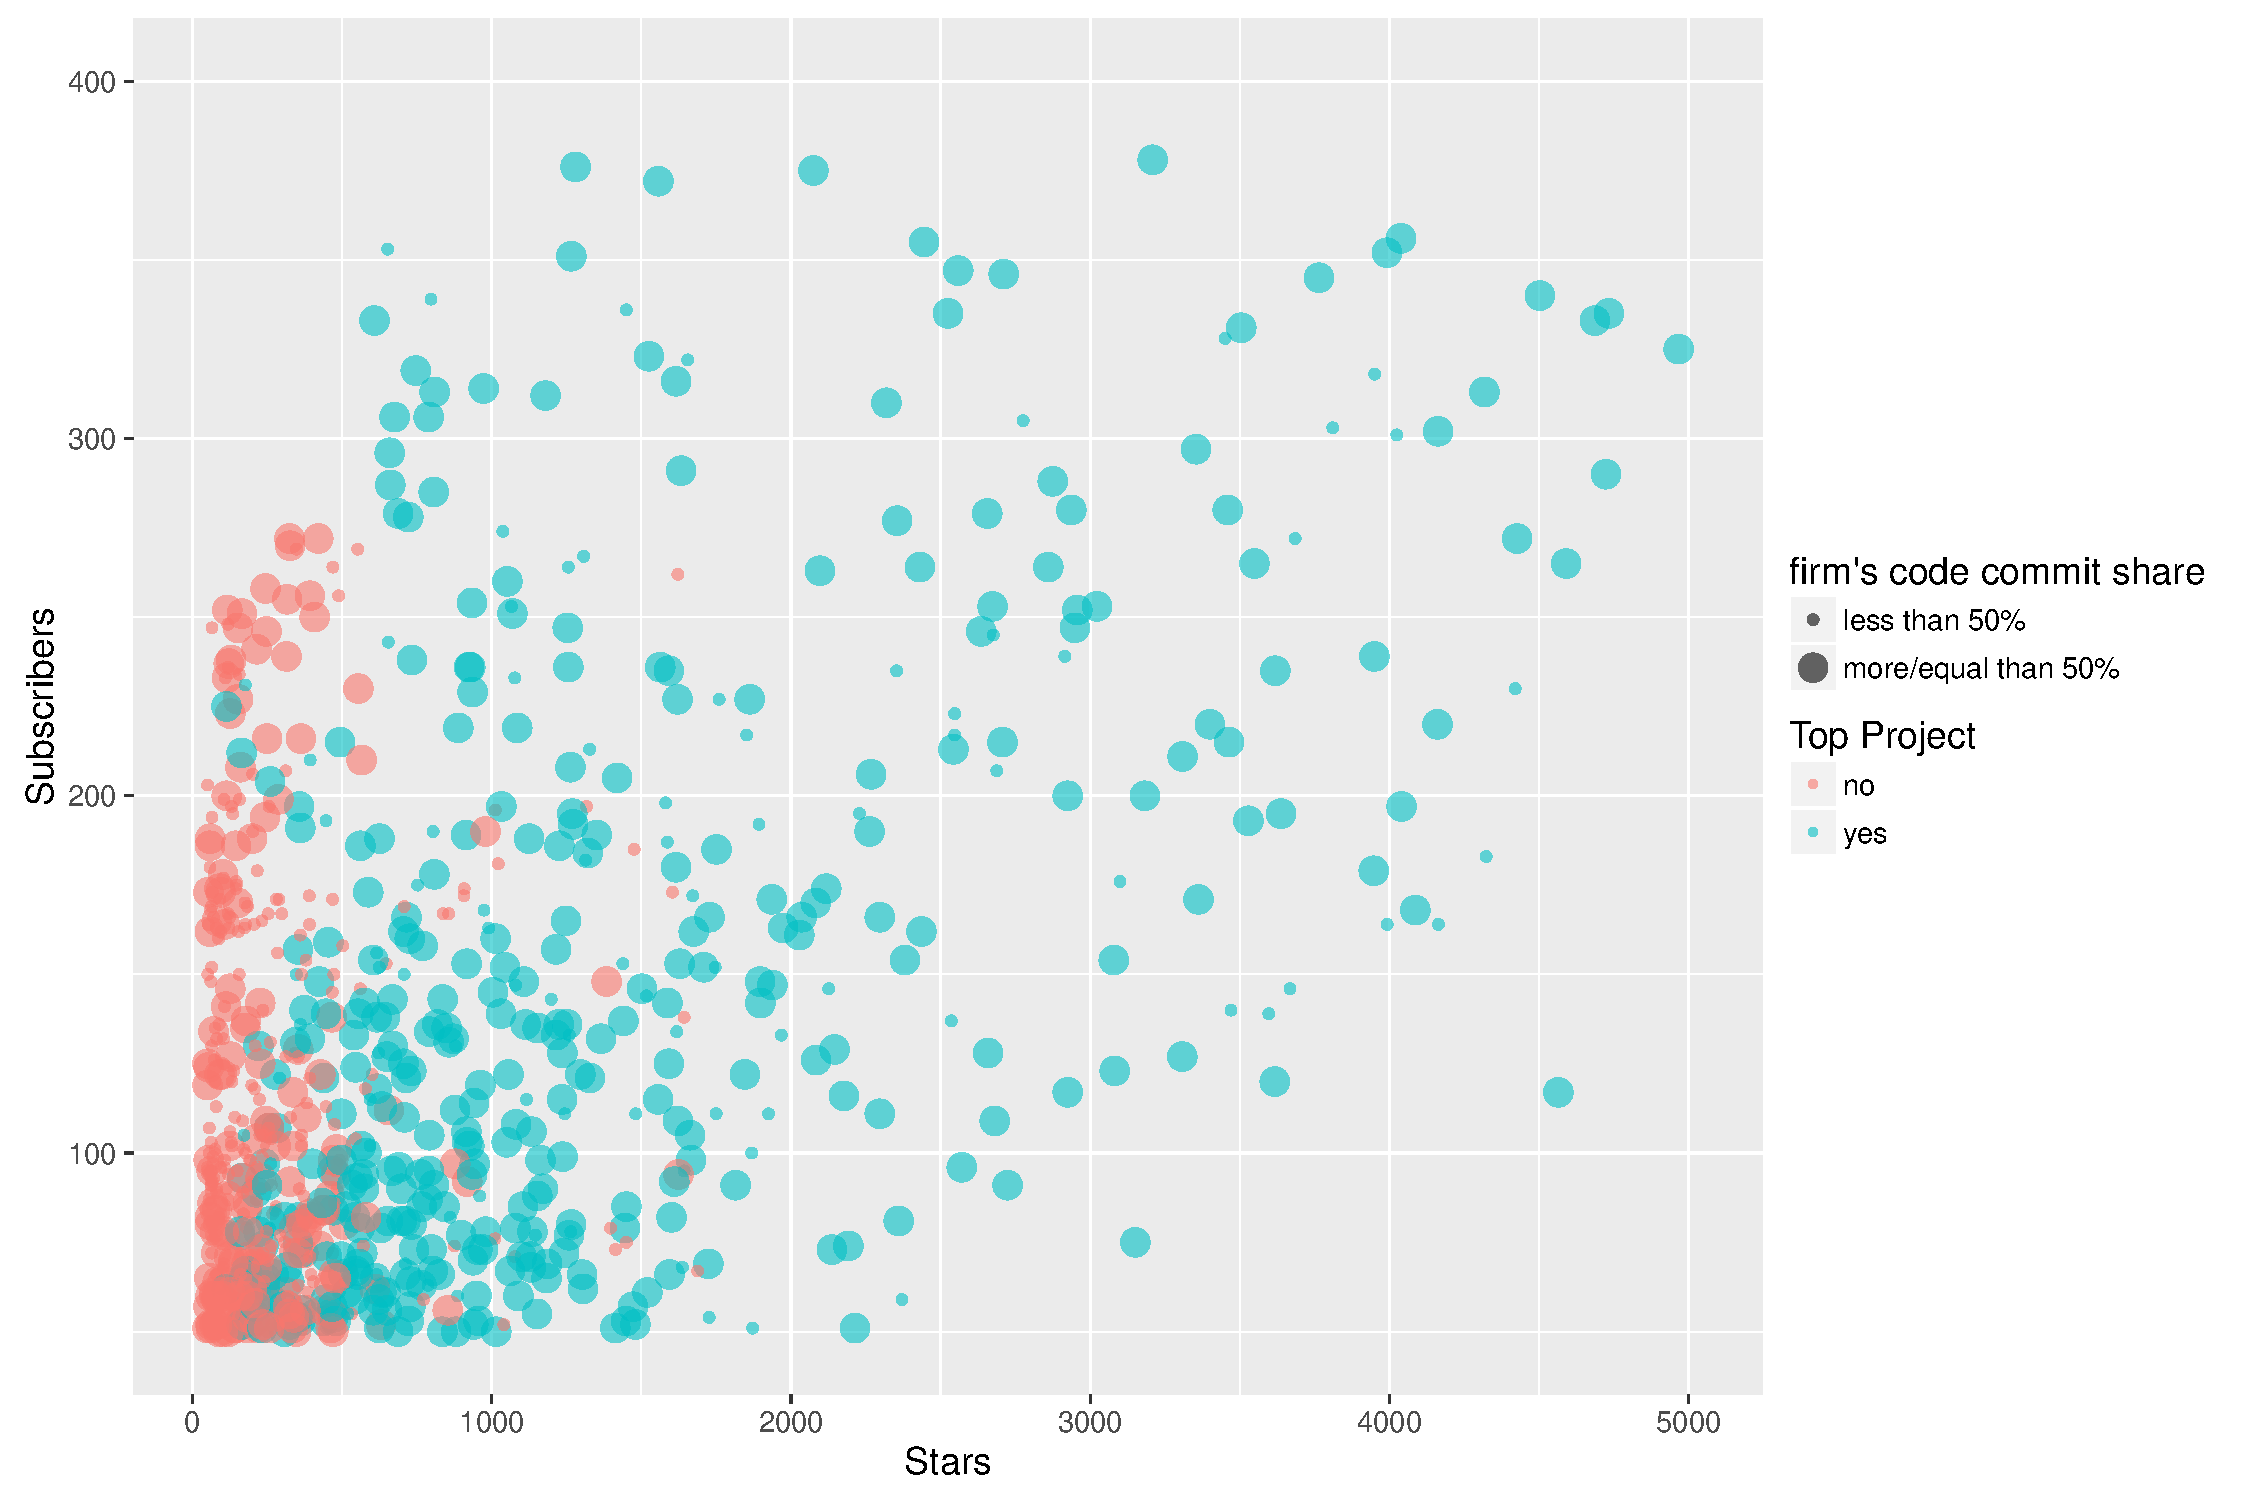
\includegraphics[page=1,scale=0.4]{../graphics/intro/stars_subscribers_ratio_top_5000.pdf}
	\caption{Same as figure \ref{fig:stars_subscribers_ratio_top_10000} but with scaled x-axis up to 5000 stars.}
	\label{fig:stars_subscribers_ratio_top_5000}
\end{figure}

\begin{figure}
	\centering
	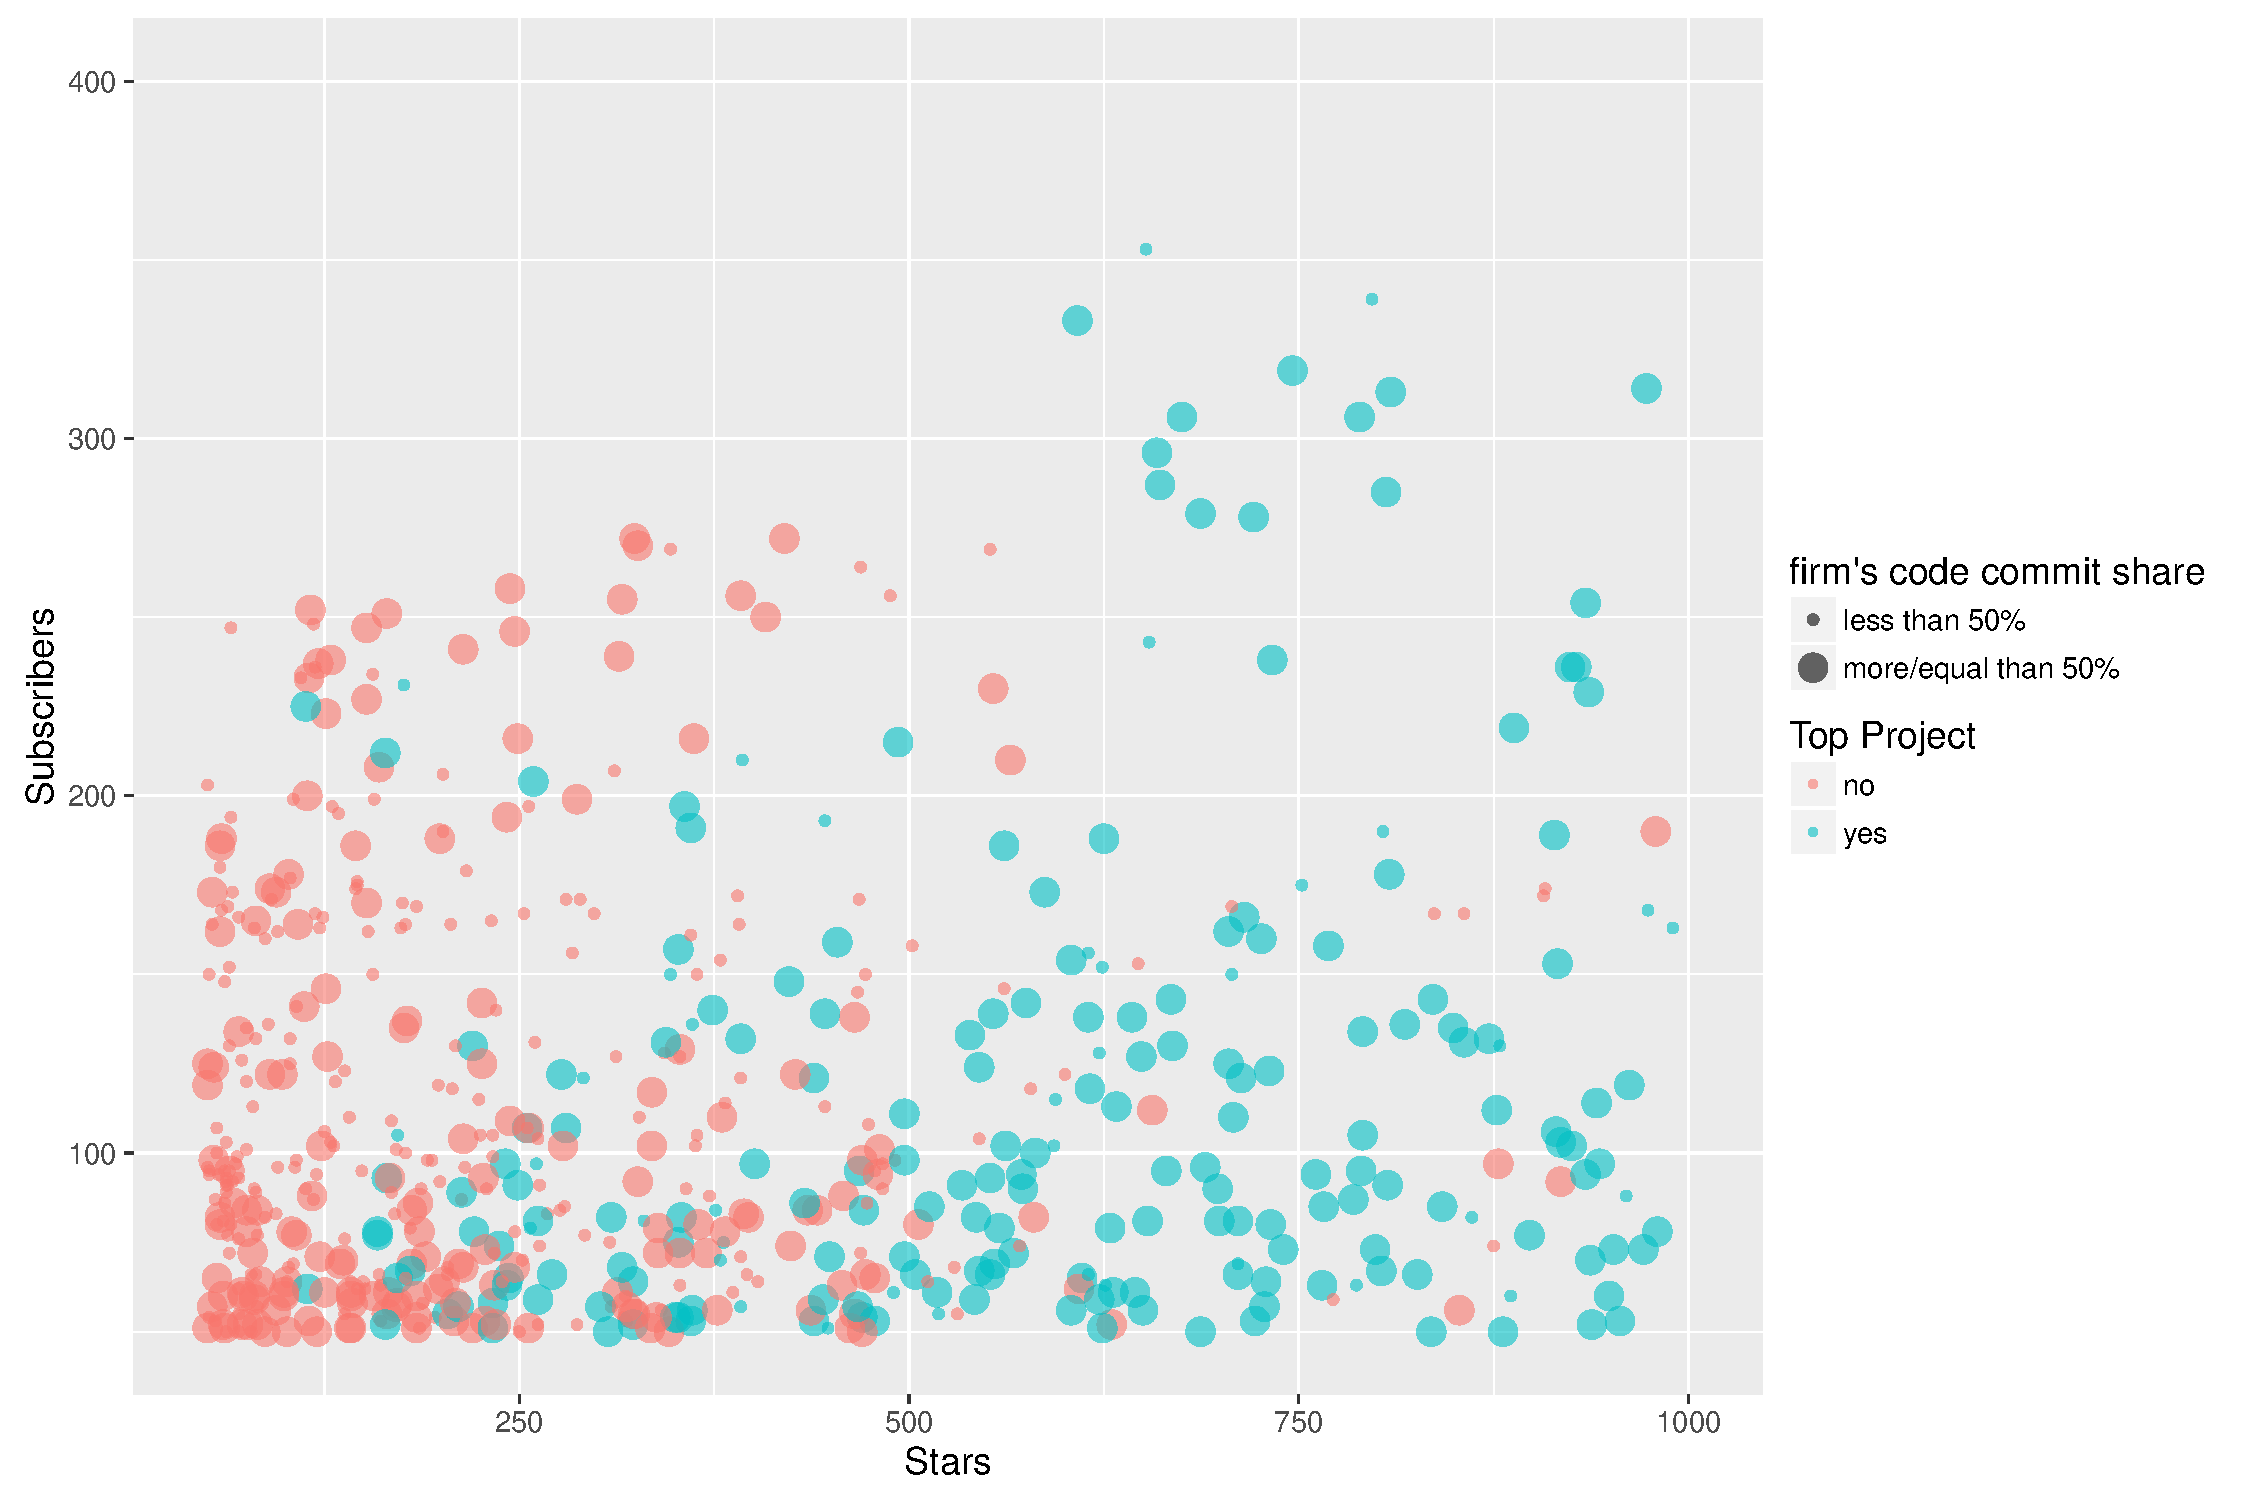
\includegraphics[page=1,scale=0.4]{../graphics/intro/stars_subscribers_ratio_top_1000.pdf}
	\caption{Same as figure \ref{fig:stars_subscribers_ratio_top_10000} but with scaled x-axis up to 1000 stars.}
	\label{fig:stars_subscribers_ratio_top_1000}
\end{figure}

\end{landscape}







\subsection{Plots for H 1.1}
\label{sec:h_1.1_plots}

See page \pageref{sec:lm_plots_description} for explanation of slopes and axes.

\vspace{20 pt}

\begin{minipage}{.5\textwidth}
	\centering
	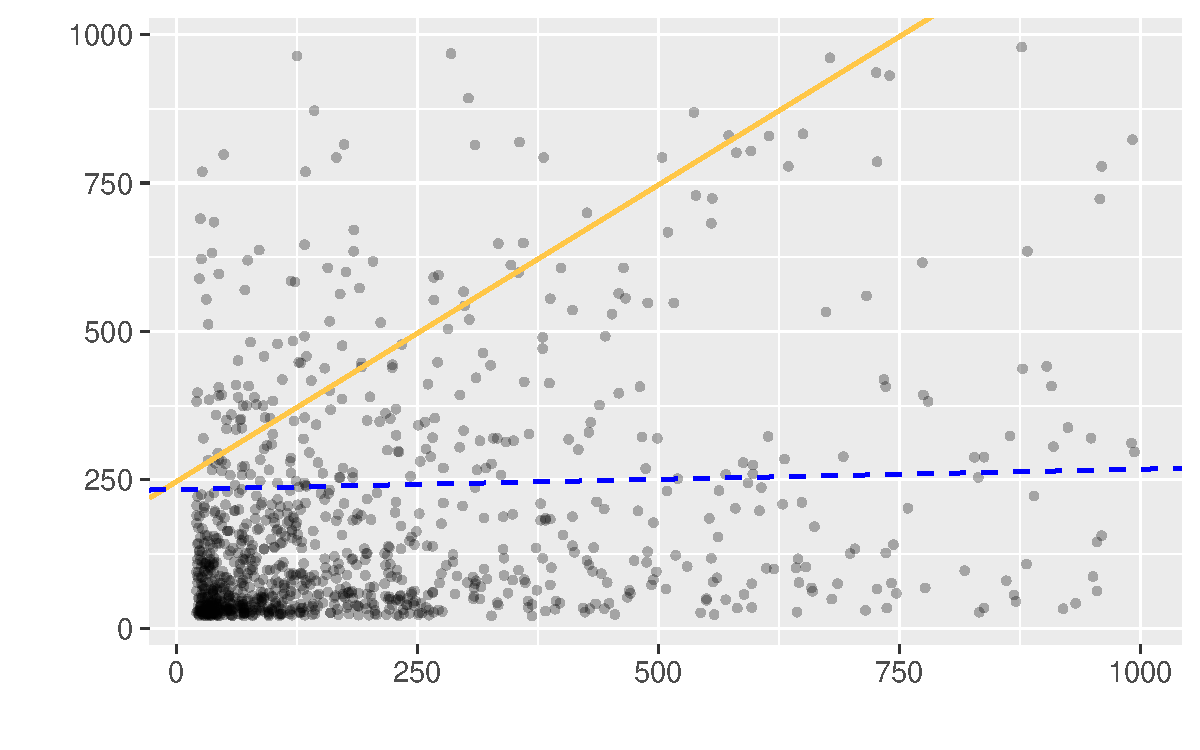
\includegraphics[page=1,scale=0.3]{../hypotheses/lm_in_ext_model_1_2.pdf}
  \captionof{figure}{All Projects (Model 1.1.1 - 1.1.2)}
  \label{fig:hyp1_model_1-2}
\end{minipage}
\begin{minipage}{.5\textwidth}
	\centering
	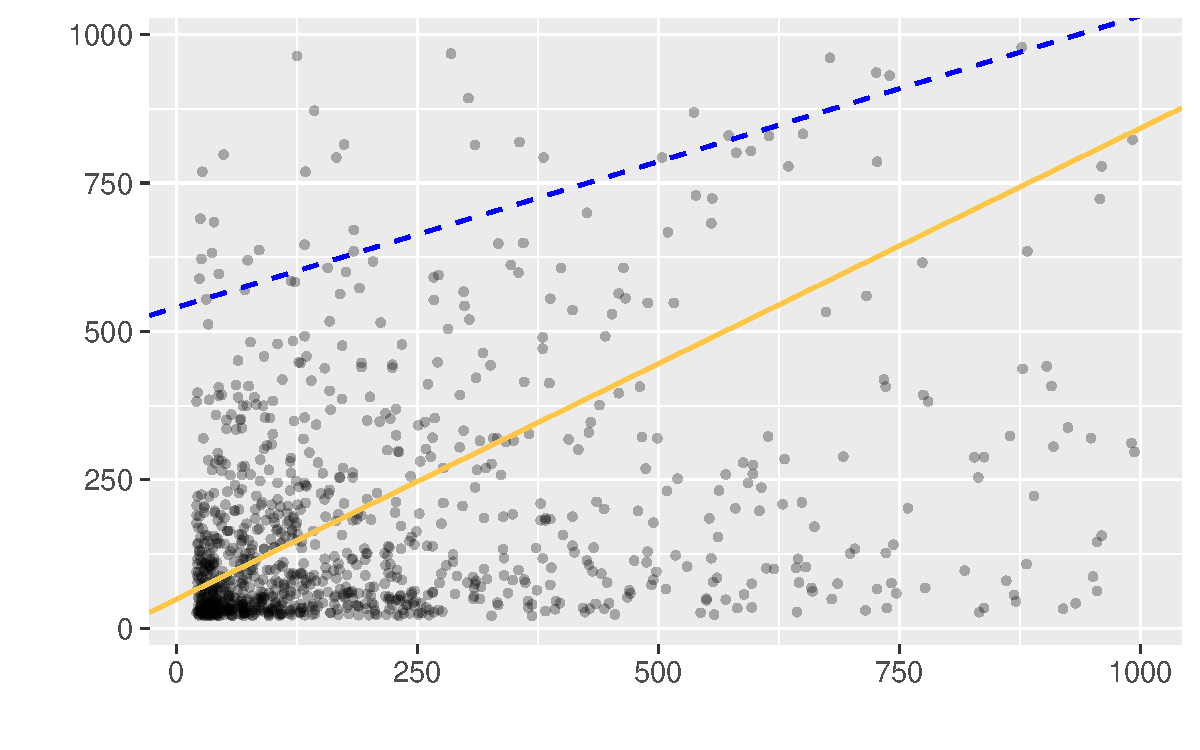
\includegraphics[page=1,scale=0.3]{../hypotheses/lm_in_ext_model_3_4.pdf}
  \captionof{figure}{Top Projects (Model 1.1.3 - 1.1.4)}
  \label{fig:hyp1_model_3-4}
\end{minipage}

\vspace{20 pt}

\begin{minipage}{.5\textwidth}
	\centering
	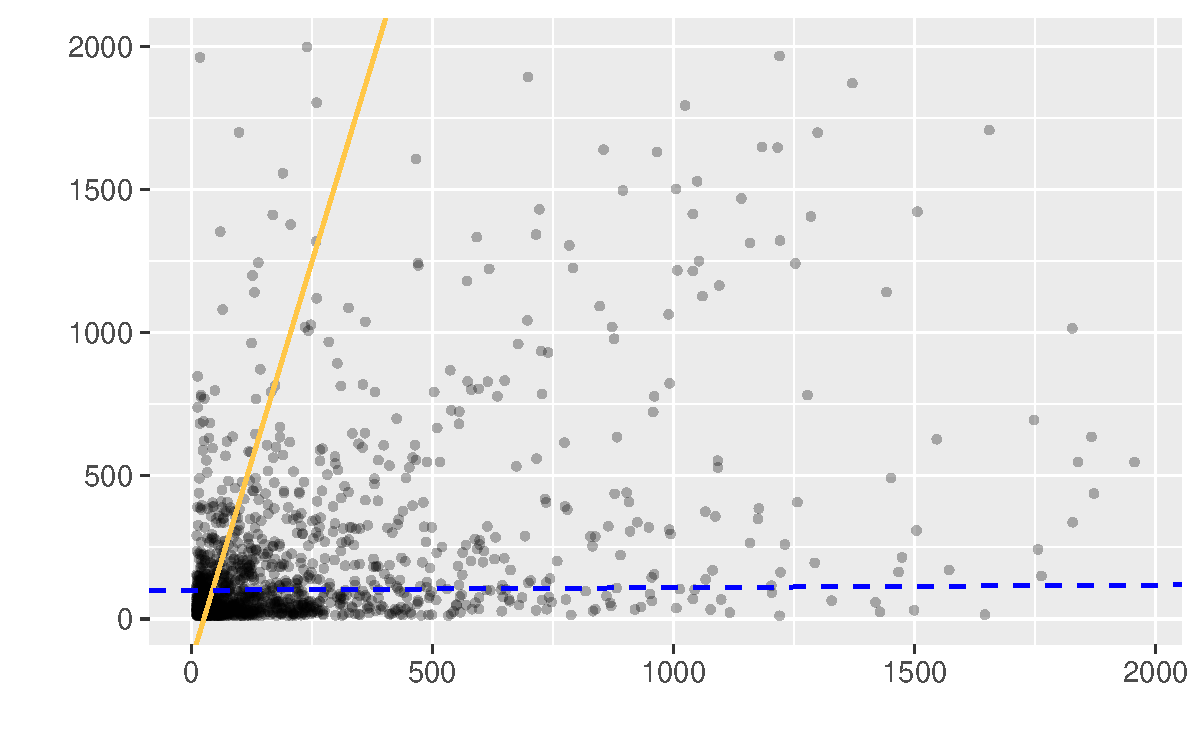
\includegraphics[page=1,scale=0.3]{../hypotheses/lm_in_ext_model_5_6.pdf}
  \captionof{figure}{Residual Projects (Model 1.1.5 - 1.1.6)}
  \label{fig:hyp1_model_5-6}
\end{minipage}
\begin{minipage}{.5\textwidth}
	\centering
	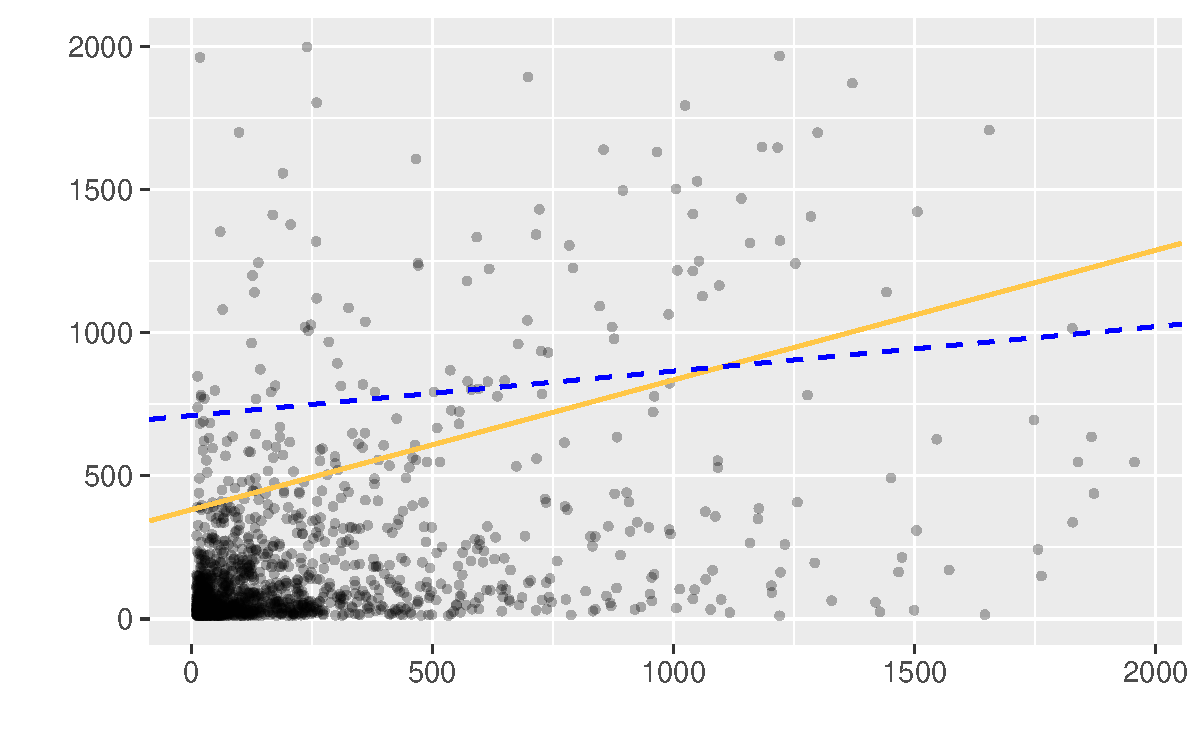
\includegraphics[page=1,scale=0.3]{../hypotheses/lm_in_ext_model_7_8.pdf}
  \captionof{figure}{Older Top Projects (Model 1.1.7 - 1.1.8)}
  \label{fig:hyp1_model_7-8}
\end{minipage}

\vspace{20 pt}

\begin{minipage}{.5\textwidth}
	\centering
	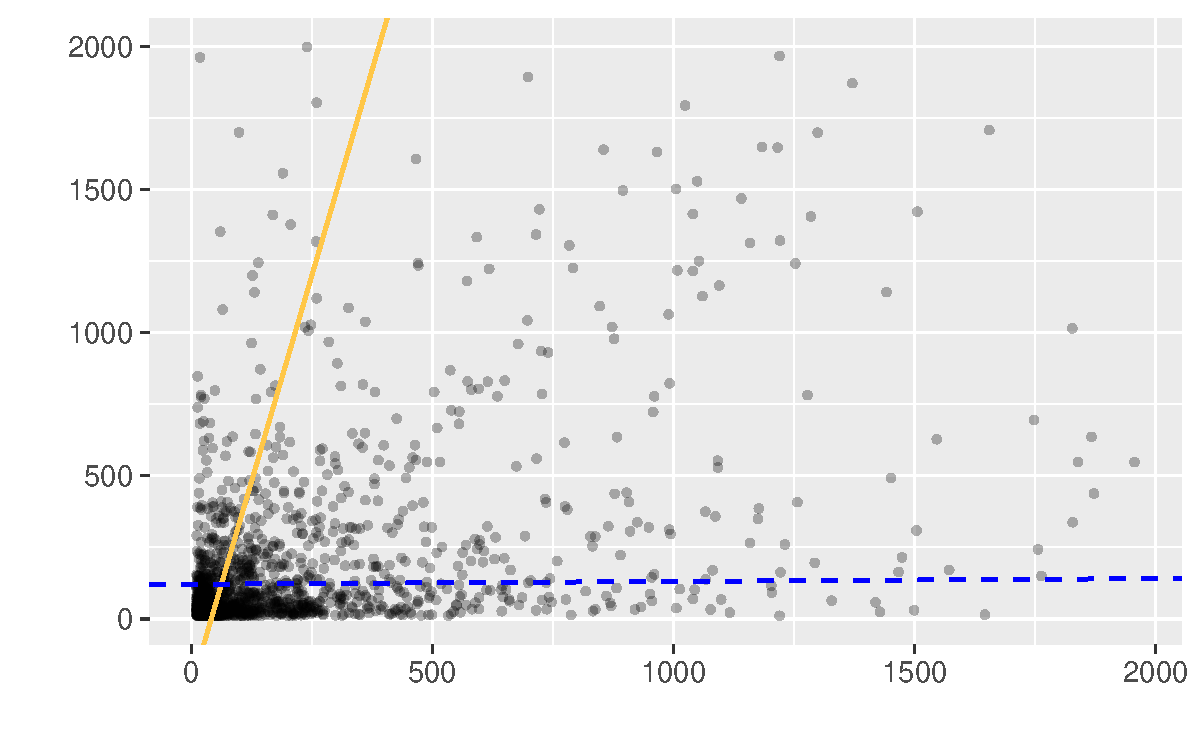
\includegraphics[page=1,scale=0.3]{../hypotheses/lm_in_ext_model_9_10.pdf}
  \captionof{figure}{Older Residual Projects (Model 1.1.9  - 1.1.10)}
  \label{fig:hyp1_model_9-10}
\end{minipage}
\begin{minipage}{.5\textwidth}
	\centering
	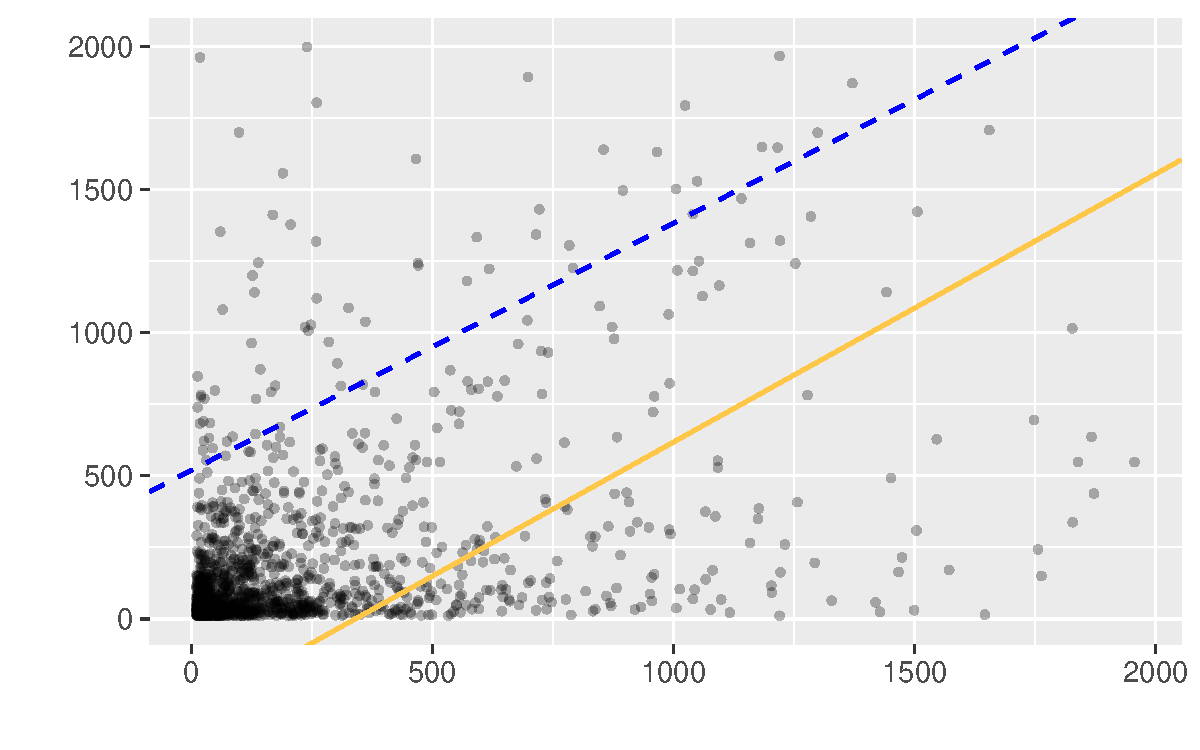
\includegraphics[page=1,scale=0.3]{../hypotheses/lm_in_ext_model_11_12.pdf}
  \captionof{figure}{Younger Top Projects (Model 1.1.11 - 1.1.12)}
  \label{fig:hyp1_model_11-12}
\end{minipage}





\subsection{Plots for H 1.2.1}
\label{sec:h_1.2.1_plots}

See page \pageref{sec:lm_plots_description} for explanation of slopes and axes.

\vspace{20 pt}

\begin{minipage}{.5\textwidth}
	\centering
	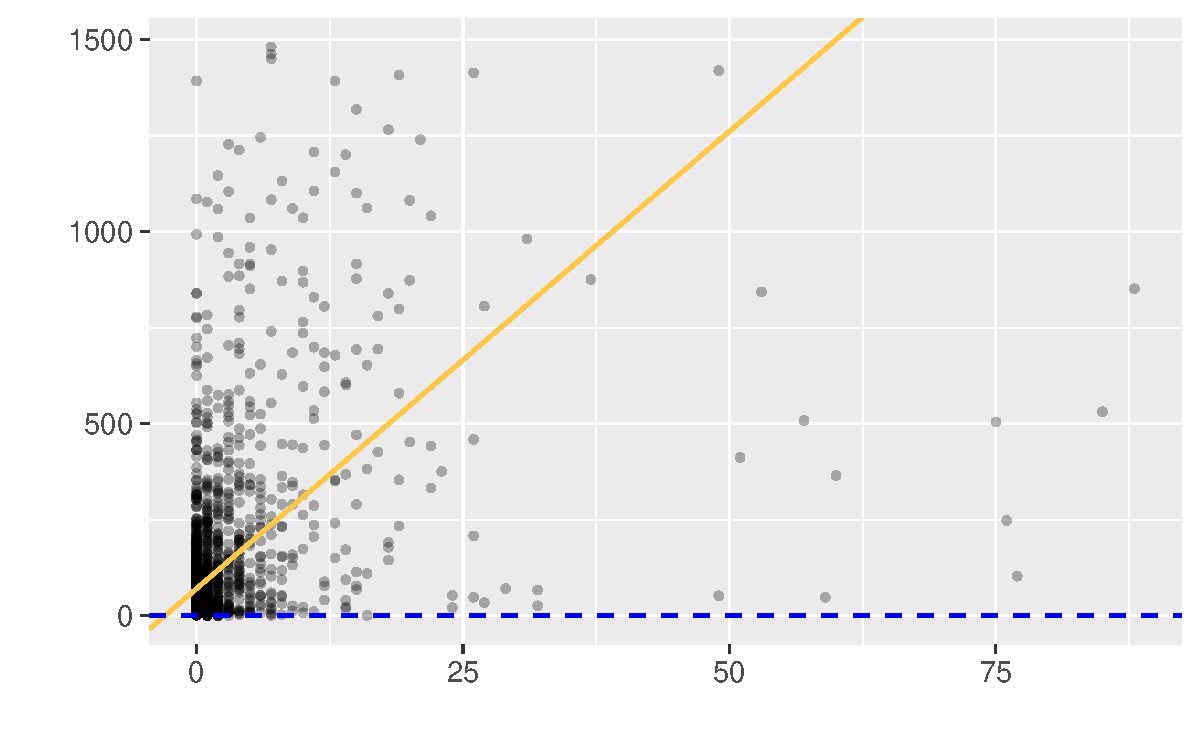
\includegraphics[page=1,scale=0.3]{../hypotheses/lm_issues_model_1_2.pdf}
  \captionof{figure}{All Projects (Model 1.2.1 - 1.2.2)}
  \label{fig:hyp1_issue_model_1-2}
\end{minipage}
\begin{minipage}{.5\textwidth}
	\centering
	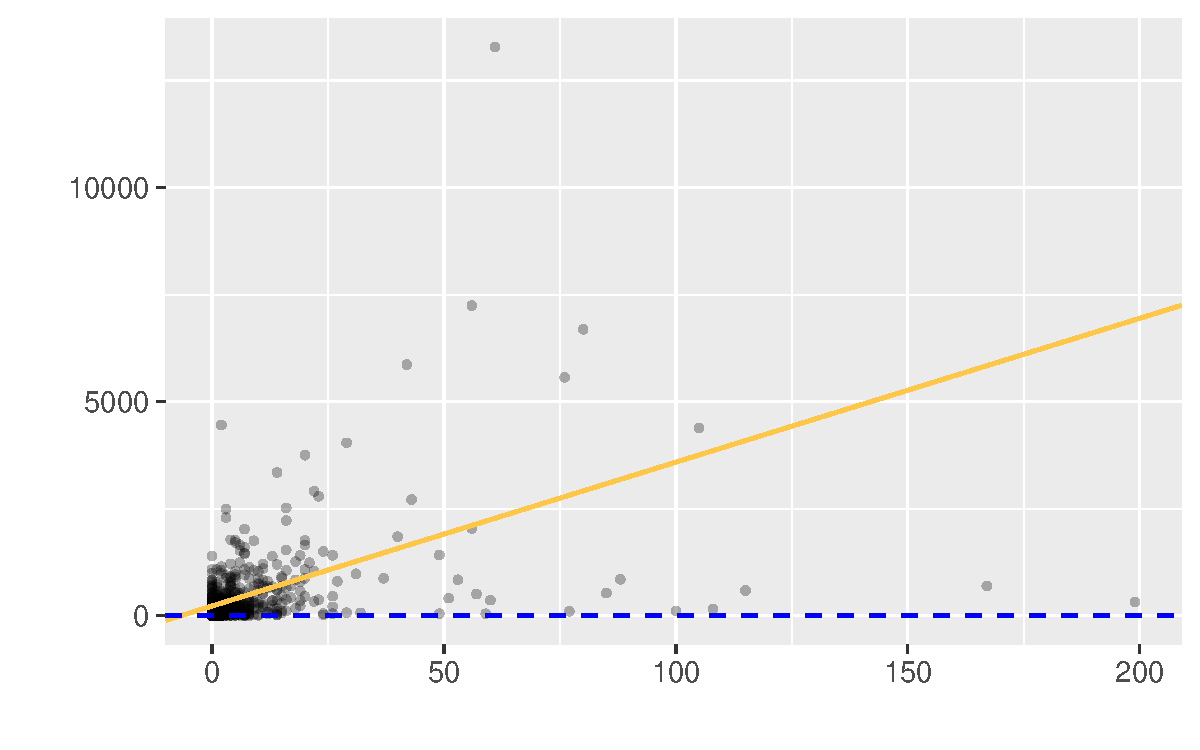
\includegraphics[page=1,scale=0.3]{../hypotheses/lm_issues_model_3_4.pdf}
  \captionof{figure}{Top Projects (Model 1.2.3 - 1.2.24)}
  \label{fig:hyp1_issue_model_3-4}
\end{minipage}

\vspace{20 pt}

\begin{minipage}{.5\textwidth}
	\centering
	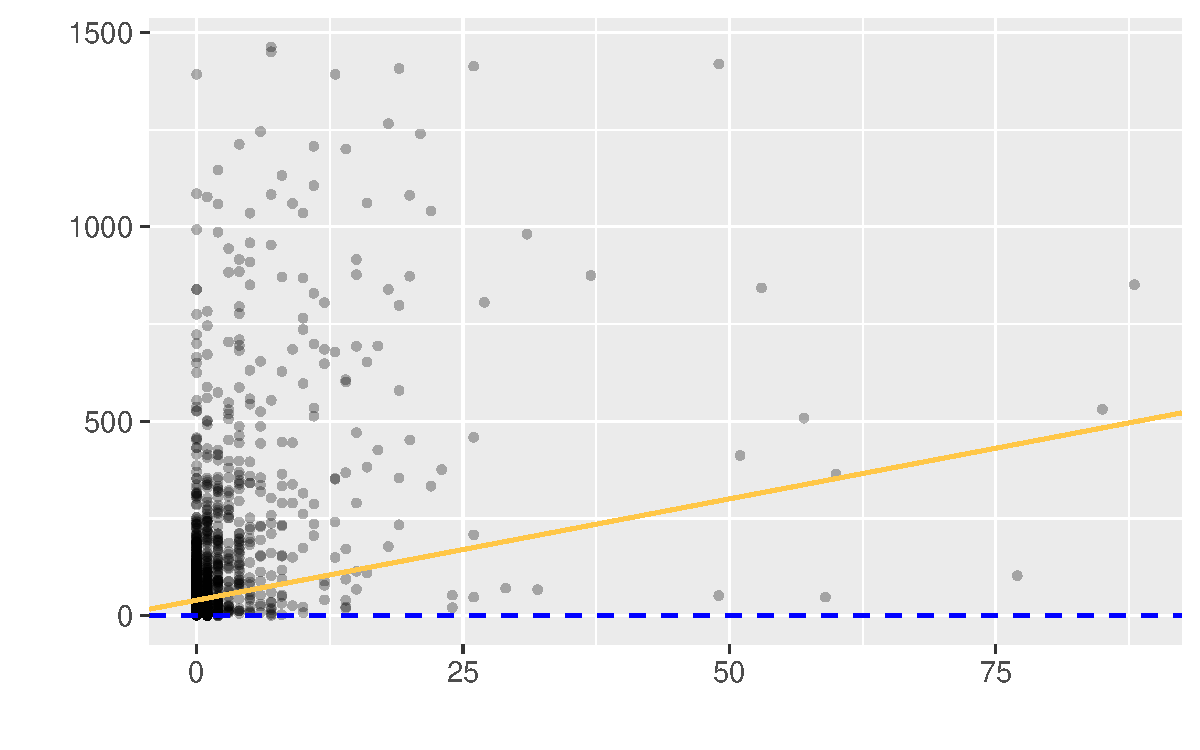
\includegraphics[page=1,scale=0.3]{../hypotheses/lm_issues_model_5_6.pdf}
  \captionof{figure}{Residual Projects \newline (Model 1.2.5 - 1.2.6)}
  \label{fig:hyp1_issue_model_5-6}
\end{minipage}
\begin{minipage}{.5\textwidth}
	\centering
	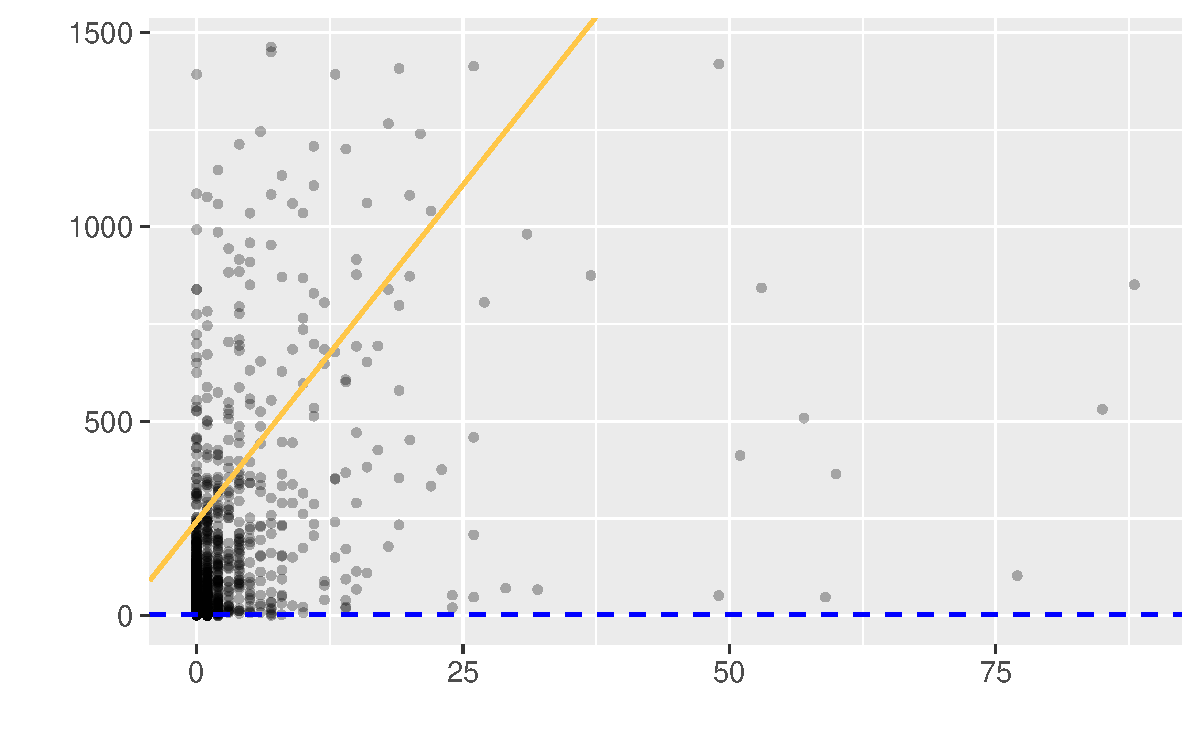
\includegraphics[page=1,scale=0.3]{../hypotheses/lm_issues_model_7_8.pdf}
  \captionof{figure}{Older Top Projects \newline (Model 1.2.7 - 1.2.8)}
  \label{fig:hyp1_issue_model_7-8}
\end{minipage}

\vspace{20 pt}

\begin{minipage}{.5\textwidth}
	\centering
	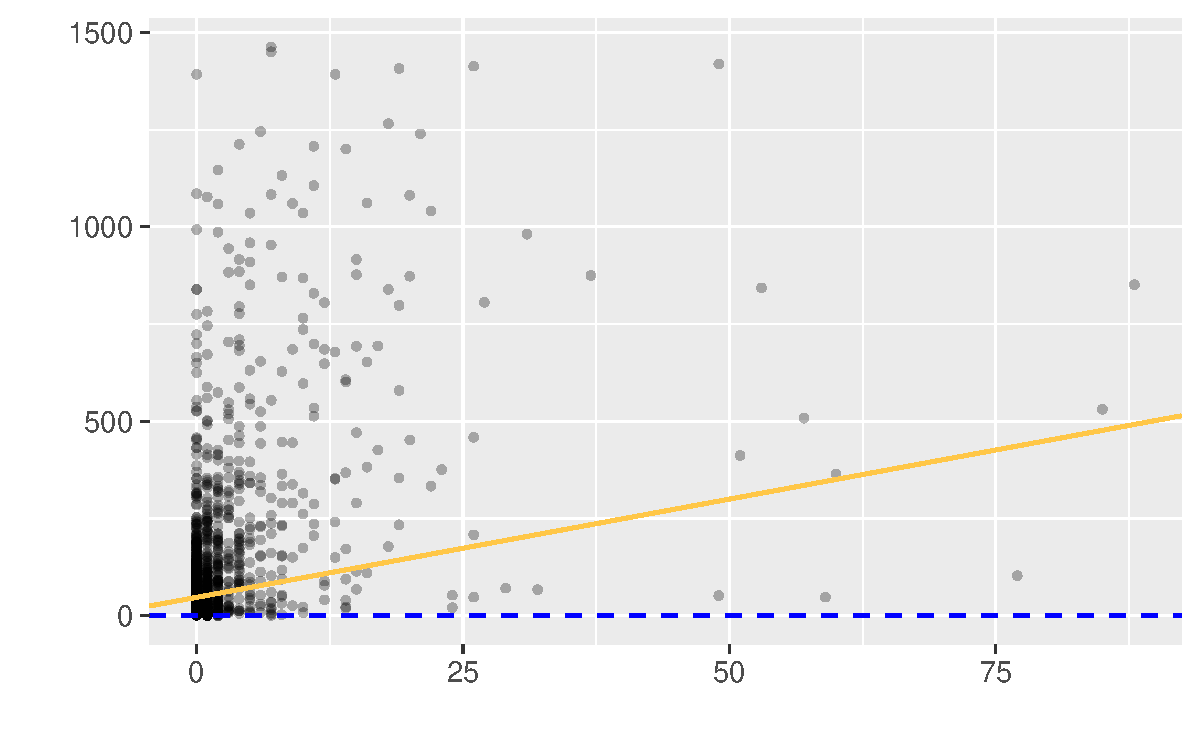
\includegraphics[page=1,scale=0.3]{../hypotheses/lm_issues_model_9_10.pdf}
  \captionof{figure}{Older Residual Projects \newline (Model 1.2.9 - 1.2.10)}
  \label{fig:hyp1_issue_model_9-10}
\end{minipage}
\begin{minipage}{.5\textwidth}
	\centering
	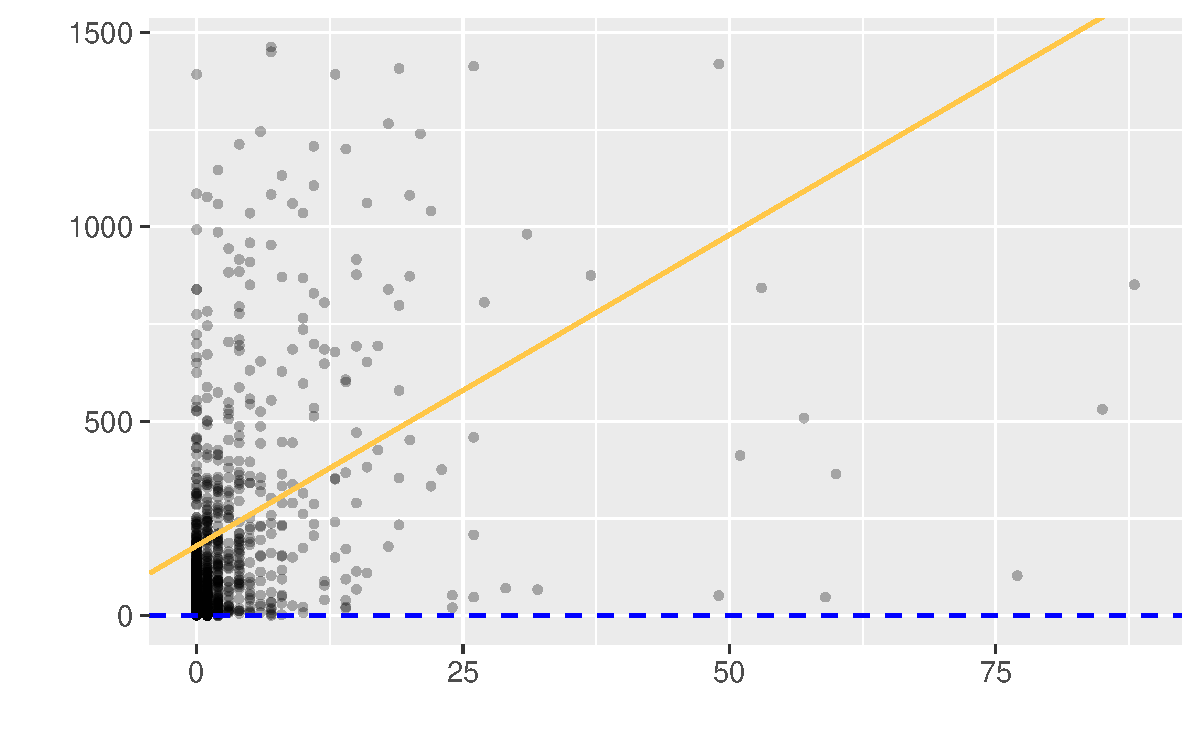
\includegraphics[page=1,scale=0.3]{../hypotheses/lm_issues_model_11_12.pdf}
  \captionof{figure}{Younger Top Projects \newline (Model 1.2.11 - 1.2.12)}
  \label{fig:hyp1_issue_model_11-12}
\end{minipage}

\vspace{20 pt}

\begin{minipage}{.5\textwidth}
	\centering
	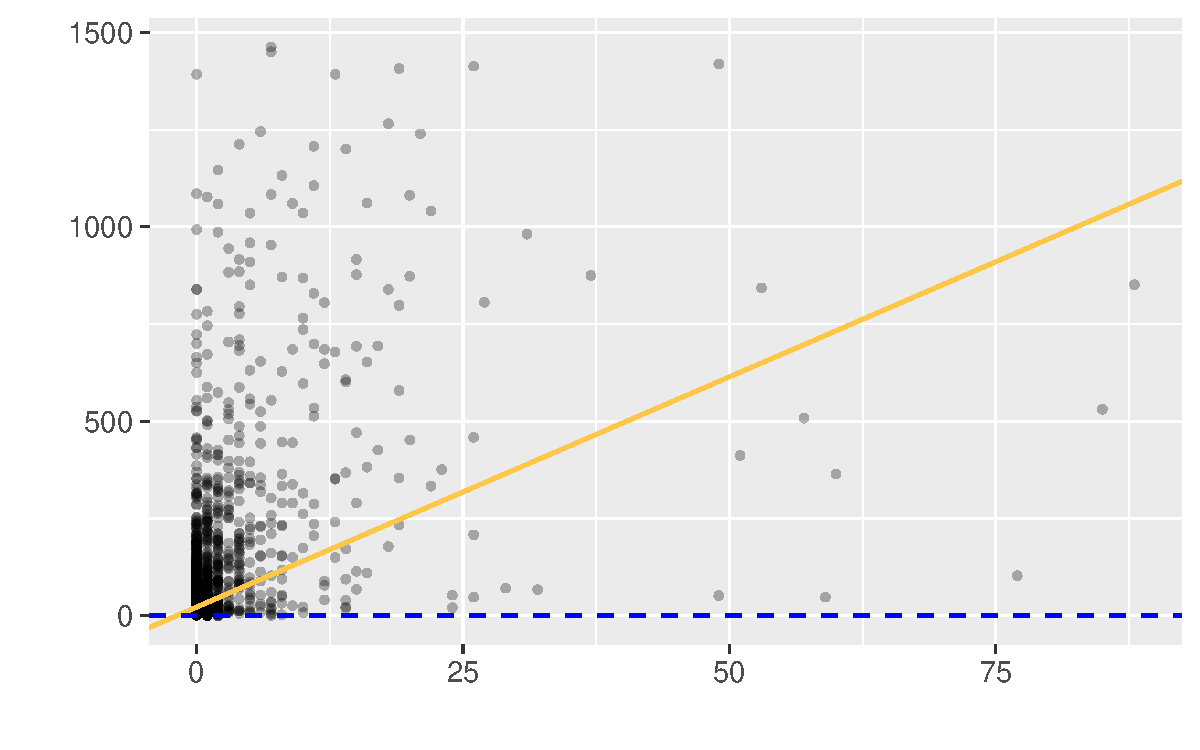
\includegraphics[page=1,scale=0.3]{../hypotheses/lm_issues_model_13_14.pdf}
  \captionof{figure}{Younger Residual Projects \newline (Model 1.2.13 - 1.2.14)}
  \label{fig:hyp1_issue_model_13-14}
\end{minipage}


\subsection{Plots for H 1.2.2}
\label{sec:h_1.2.2_plots}

See page \pageref{sec:lm_plots_description} and \pageref{sec:h1.2.2_models} for explanation of slopes and axes.
\vspace{20 pt}

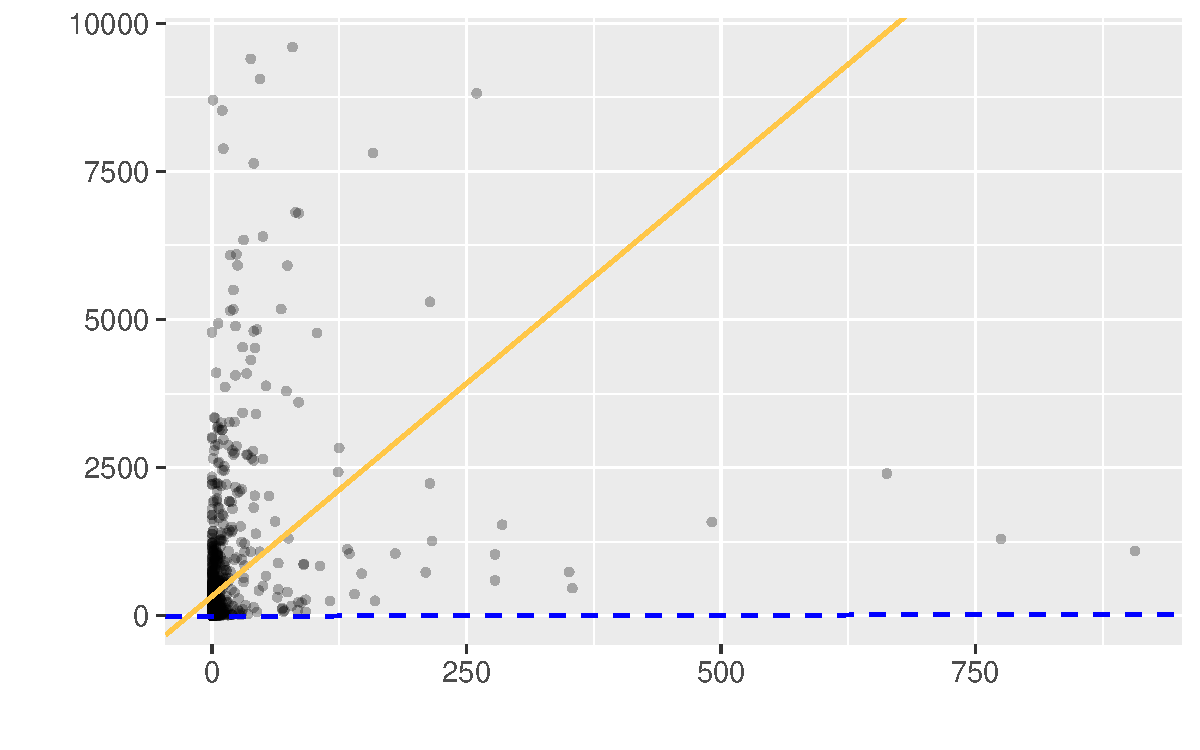
\includegraphics[page=1,scale=0.7]{../hypotheses/h1_issue_comments_all.pdf}
\captionof{figure}{Comments of Issues (Model 1.3.3- 1.3.4)}
\label{fig:hyp1_issuecomments_top_model_3}
\vspace{20 pt}
\begin{minipage}{.5\textwidth}
	\centering
	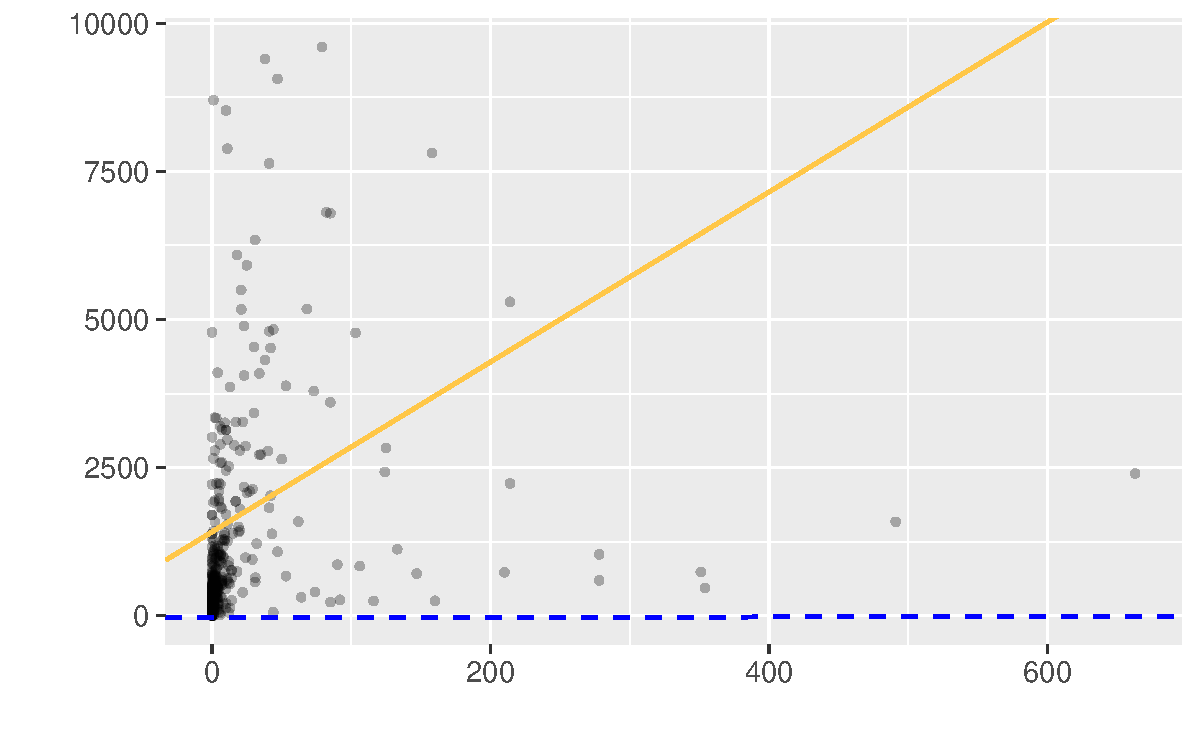
\includegraphics[page=1,scale=0.3]{../hypotheses/h1_issue_comments_top.pdf}
  \captionof{figure}{Comments of Issues \newline (Model 1.3.3- 1.3.4)}
  \label{fig:hyp1_issuecomments_residual_model_3}
\end{minipage}
\begin{minipage}{.5\textwidth}
	\centering
	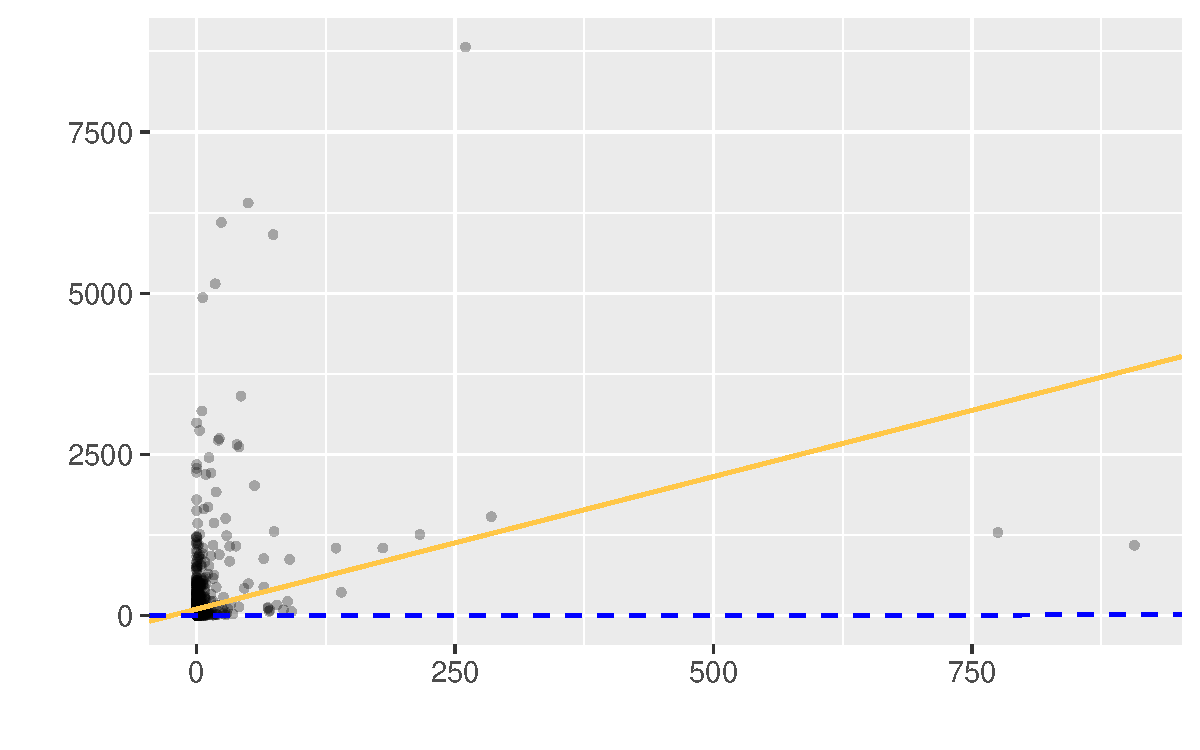
\includegraphics[page=1,scale=0.3]{../hypotheses/h1_issue_comments_residual.pdf}
  \captionof{figure}{Comments of Issues \newline (Model 1.3.5- 1.3.6)}
  \label{fig:hyp1_issuecomments_residual_model_3}
\end{minipage}


\clearpage
\newpage
\section{Open Source Software used for making this Study}

The following open source software is used to receive, process, analyze and present the data (this list is not fully inclusive):

\begin{itemize}
  \item [\textbf{Atom Editor}] (\url{https://github.com/atom/atom})
  \item [\textbf{R Studio}] (\url{https://github.com/rstudio/rstudio})
  \begin{itemize}
    \item [foreign] (\cite{R_foreign})
    \item [MASS] (\cite{R_MASS})
    \item [xtable] (\cite{R_xtable})
    \item [stargazer] (\cite{R_stargazer})
    \item [stringr] (\cite{R_stringr})
    \item [ggplot2] (\cite{R_ggplot2})
    \item [scales] (\cite{R_scales})
    \item [PerformanceAnalytics] (\cite{R_PerformanceAnalytics})
    \item [xts] (\cite{R_xts})
    \item [TeachingDemos] (\cite{R_TeachingDemos})
  \end{itemize}
  \item [\textbf{NodeJS}] (\url{https://github.com/nodejs/node}) using the following npm modules:
  \begin{itemize}
    \item [csv] (0.4.6)
    \item [csv-stringify] (v0.0.8)
    \item [coffee-script] (v1.9.0)
    \item [fast-csv] (v0.6.0)
    \item [github] (v0.2.4)
    \item [glob] (v6.0.4)
    \item [globs] (v0.1.2)
    \item [google] (v1.4.0)
    \item [js-yaml] (v3.4.3)
    \item [kerberos] (v0.0.18)
    \item [minimist] (v1.2.0)
    \item [moment] (v2.10.6)
    \item [moment-timezone] (v0.4.1)
    \item [mongodb] (v2.1.7)
    \item [mongoskin] (v2.0.0)
    \item [nodemailer] (v1.8.0)
    \item [procstreams] (v0.3.0)
    \item [progress] (v1.1.8)
    \item [request] (v2.61.0)
    \item [sequence] (v3.0.0)
    \item [split] (v1.0.0)
    \item [underscore] (v1.8.3)
    \item [yargs] (v3.27.0)
  \end{itemize}
  \item [\textbf{MariaDB}] (\url{https://github.com/MariaDB/server})
  \item [\textbf{MongoDB}] (\url{https://github.com/mongodb/mongo})
  \item [\textbf{Texmaker}] (\url{http://www.xm1math.net/texmaker/download.html})
  \item [\textbf{\LaTeX}] (\url{https://www.latex-project.org/})
\end{itemize}


\newpage
\normalsize
% literature
\addcontentsline{toc}{section}{References}
\bibliography{literature,theory,r}
% \bibliography{theory}


% figures (not mandatory)
%%\newpage
%%\input{app_figures}



% --------------------------------------------
% --- last page: Declaration of Authorship ---
% --------------------------------------------

%\newpage
%\thispagestyle{empty}
%\normalsize
%\input{authorship}


\end{document}
